\documentclass[aspectratio=1610,xcolor=svgnames]{beamer}

\usetheme{metropolis}

\usepackage{appendixnumberbeamer}
\usepackage{tikz}
\usepackage{varwidth}
\usepackage[absolute,overlay]{textpos}
\usepackage{pstricks}
%\usepackage[texcoord,grid,gridunit=mm,gridcolor=red!10,subgridcolor=green!10]{eso-pic}

\usetikzlibrary{patterns}
\usetikzlibrary{shapes}
\usetikzlibrary{shapes.symbols}
\usetikzlibrary{fit}
\usetikzlibrary{backgrounds}
\usetikzlibrary{calc}

\newcommand{\tikzdbg}{%
  \draw[step=1,color=lightgray] (-7,0) grid (7,7);%
  \fill[red] (0,0) circle (0.2);%
}


\title{Deadline scheduling in the Linux kernel}
\subtitle{Juri Lelli, Claudio Scordino, Luca Abeni and Dario Faggioli}
\date{July 8, 2019}
\author{Benno Fünfstück}

\begin{document}

%\includeonlyframes{current}

\pgfmathsetmacro{\taskheight}{0.4cm}
\pgfmathsetmacro{\taskunit}{0.9}
\colorlet{brew}{olive}
\colorlet{ui}{black!80!white}
\colorlet{web}{teal}

\tikzset{
  onslide/.code args={<#1>#2}{%
    \only<#1>{\pgfkeysalso{#2}}% \pgfkeysalso doesn't change the path
  },
  temporal/.code args={<#1>#2#3#4}{%
    \temporal<#1>{\pgfkeysalso{#2}}{\pgfkeysalso{#3}}{\pgfkeysalso{#4}}%
  },
  hidden/.style = {opacity=0},
  uncover/.style = {temporal=#1{hidden}{}{hidden}},
  task inactive/.style = {pattern=north west lines,pattern color=#1!80!white, draw=#1!80!white},
  task active/.style = {fill=#1,draw=#1},
}

\newcommand{\task}[4]{%
  \path[task #1=#2] (#3*\taskunit,0.0) rectangle +(#4*\taskunit, \taskheight+0cm);%
}
\newcommand{\period}[1]{%
  \draw[color=alert,<->,thick] (#1*\taskunit,0.0) -- +(0,0.6cm);%
}
\newcommand{\taskstart}[0]{%
  \draw[color=alert,->,thick] (0,0.0) -- +(0,0.6cm);%
}

\maketitle

\begin{frame}\frametitle{Story: A new coffee machine}
  \vspace{1cm}
  \begin{columns}
    \begin{column}{0.5\textwidth}
      
\includegraphics[width=0.95\textwidth]{coffee.pdf}
    \end{column}
    \begin{column}{0.5\textwidth}
      {\Large Components:}
      \begin{itemize}
      \item Brewing controller
      \item User interface controller
      \item Web interface
      \end{itemize}
      \vspace{0.5cm}
      \pause
      {\Large $\Rightarrow$ real-time tasks} \\
      (guaranteed worst-case response time)
    \end{column}
  \end{columns}
\end{frame}

\begin{frame}\frametitle{Linux for real-time}
  First approach: run Linux as a task in real-time hypervisor
  \begin{itemize}
  \item examples: RTAI, RTLinux, Xenomai
  \item maintenance of HAL and microkernel for real-time
  \item custom tools and API necessary for real-time part 
  \end{itemize}

  \pause

  Second approach: make the Linux kernel itself suitable for real-time
  \begin{itemize}
  \item PREEMPT\_RT patchset
  \item<3-> \alert{real-time scheduler}
  \end{itemize}
\end{frame}

\section{Design of a realtime scheduler}

% \begin{frame}\frametitle{Real-time Tasks}
%   Properties of real-time tasks: \textit{runtime}, \textit{deadline} and \textit{period}

%   For our coffee machine:

%   \begin{tikzpicture}
%     % draw time axis
%     \draw[->] (-6.1,1) -- (5,1) node[below,xshift=-0.4cm]{time in ms};
%     \foreach \x in {0,5,10} \draw[line width=1.3pt] (-6+\x*\taskunit,1.05) -- (-6+\x*\taskunit,0.95);
%     \foreach \x in {0,...,10} {
%       \pgfmathsetmacro{\ms}{int(\x*20)};
%       \draw (-6+\x*\taskunit,1.05) -- (-6+\x*\taskunit,0.95) node[anchor=north]{\ms};
%     }
%     \foreach \x in {0,...,12} {
%       \draw[thin, gray, dashed] (-6+\x*\taskunit,1) -- (-6+\x*\taskunit,4);
%     }

%     % draw the task labels
%     \begin{scope}[anchor=south east, rectangle, xshift=-6cm, minimum height=\taskheight]
%       \node[yshift=1.5cm, label=west:{web (10/200)}] {};
%       \node[yshift=2.5cm, label=west:{UI (10/40)}] {};
%       \node[yshift=3.5cm, label=west:{brew (40/100)}] {};
%     \end{scope}

%     % draw the tasks
%     \begin{scope}[xshift=-6cm, yshift=1.5cm]
%       \clip (-0.2,0) rectangle (11,3);

%       \begin{scope}
%         \task{inactive}{web}{0}{3};
%         \task{active}{web}{3}{0.5};
%         \task{inactive}{web}{10}{3};
%         \taskstart;
%         \period{10};
%       \end{scope}

%       \begin{scope}[yshift=1cm]
%         \foreach \t in {0,2,...,12} \task{active}{ui}{\t}{0.5};
%         \taskstart;
%         \foreach \d in {2,4,...,12} \period{\d};
%       \end{scope}

%       \begin{scope}[yshift=2cm]
%         \task{inactive}{brew}{0}{0.5};
%         \task{active}{brew}{0.5}{1.5};
%         \task{inactive}{brew}{2}{0.5};
%         \task{active}{brew}{2.5}{0.5};
%         \task{active}{brew}{5}{1};
%         \task{inactive}{brew}{6}{0.5};
%         \task{active}{brew}{6.5}{1};
%         \task{inactive}{brew}{10}{0.5};
%         \task{active}{brew}{10.5}{1.5};
%         \task{inactive}{brew}{12}{0.5};
%         \taskstart;
%         \foreach \d in {5,10} \period{\d};
%       \end{scope}
%     \end{scope}
%   \end{tikzpicture}
% \end{frame}
\begin{frame}\frametitle{Linux modular scheduling framework}
  Since Linux 2.6.23 \\
  \begin{center}
    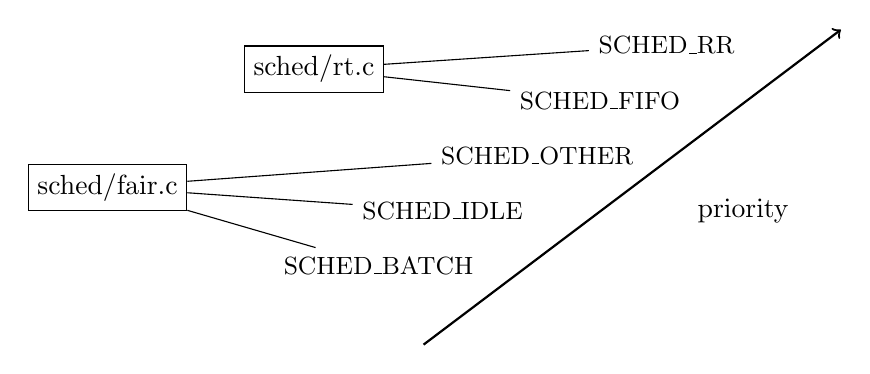
\begin{tikzpicture}
      \node[draw,rectangle,anchor=east] (rt) at (-0.5,3.5) {sched/rt.c};
      \node[draw,rectangle,anchor=east] (fair) at (-3,2.0) {sched/fair.c};
      \draw[thick,->] (0,0.0) -- (5.3,4) node[midway,right=0.7cm,yshift=-0.3cm]{priority};
      \begin{scope}[xshift=-1.9cm, yshift=1cm]
        \node[anchor=west] (rr) at (4,2.8) {\small SCHED\_RR};
        \node[anchor=west] (fifo) at (3,2.1) {\small SCHED\_FIFO};
        \node[anchor=west] (other) at (2,1.4) {\small SCHED\_OTHER};
        \node[anchor=west] (idle) at (1,0.7) {\small SCHED\_IDLE};
        \node[anchor=west] (batch) at (0,0) {\small SCHED\_BATCH};
      \end{scope}

      \draw (rt) -- (rr);
      \draw (rt) -- (fifo);
      \draw (fair) -- (other);
      \draw (fair) -- (idle);
      \draw (fair) -- (batch);
    \end{tikzpicture}
  \end{center}
\end{frame}

\begin{frame}\frametitle{Real-time Tasks}
  Properties of real-time tasks: \textit{runtime} and \textit{period}

  For our coffee machine:

  \begin{tikzpicture}
    % draw time axis
    \draw[->] (-6.1,1) -- (5,1) node[below,xshift=-0.4cm]{time in ms};
    \foreach \x in {0,5,10} \draw[line width=1.3pt] (-6+\x*\taskunit,1.05) -- (-6+\x*\taskunit,0.95);
    \foreach \x in {0,...,10} {
      \pgfmathsetmacro{\ms}{int(\x*20)};
      \draw (-6+\x*\taskunit,1.05) -- (-6+\x*\taskunit,0.95) node[anchor=north]{\ms};
    }
    \foreach \x in {0,...,12} {
      \draw[thin, gray, dashed] (-6+\x*\taskunit,1) -- (-6+\x*\taskunit,4);
    }

    % draw the task labels
    \begin{scope}[anchor=south east, rectangle, xshift=-6cm, minimum height=\taskheight]
      \node[yshift=1.5cm, label=west:{web (10/200)}] {};
      \node[yshift=2.5cm, label=west:{UI (10/40)}] {};
      \node[yshift=3.5cm, label=west:{brew (40/100)}] {};
    \end{scope}

    \only<1>{
    \begin{scope}[xshift=-6cm, yshift=1.5cm]
      \clip (-0.2,0) rectangle (11,3);

      \begin{scope}
        \task{inactive}{web}{0}{3};
        \task{active}{web}{3}{0.5};
        \task{inactive}{web}{10}{3};
        \taskstart;
        \period{10};
      \end{scope}

      \begin{scope}[yshift=1cm]
        \foreach \t in {0,2,...,12} \task{active}{ui}{\t}{0.5};
        \taskstart;
        \foreach \d in {2,4,...,12} \period{\d};
      \end{scope}

      \begin{scope}[yshift=2cm]
        \task{inactive}{brew}{0}{0.5};
        \task{active}{brew}{0.5}{1.5};
        \task{inactive}{brew}{2}{0.5};
        \task{active}{brew}{2.5}{0.5};
        \task{active}{brew}{5}{1};
        \task{inactive}{brew}{6}{0.5};
        \task{active}{brew}{6.5}{1};
        \task{inactive}{brew}{10}{0.5};
        \task{active}{brew}{10.5}{1.5};
        \task{inactive}{brew}{12}{0.5};
        \taskstart;
        \foreach \d in {5,10} \period{\d};
      \end{scope}
    \end{scope}
    }

    % draw the tasks
    \begin{scope}[xshift=-6cm, yshift=1.5cm]
      \clip (-0.2,0) rectangle (11,3);
      \alt<2->{
        \clip (-0.2,0) rectangle (12*\taskunit,3);
      }{
        \clip (-0.2,0) rectangle (3,3);
      }

      \begin{scope}
        \alt<2->{
          \task{inactive}{web}{0}{6};
        }{
          \task{inactive}{web}{0}{3};
          \task{active}{web}{3}{0.5};
        }
        \taskstart;
      \end{scope}

      \begin{scope}[yshift=1cm]
        \only<2->{
          \task{active}{ui}{0}{1.5};
          \task{active}{ui}{2}{1.5};
        }
        \foreach \t in {0,2,...,6} \task{active}{ui}{\t}{0.5};
        \taskstart;
        \foreach \d in {2,4,...,6} \period{\d};
      \end{scope}

      \begin{scope}[yshift=2cm]
        \alt<2->{
          \task{inactive}{brew}{0}{1.5};
          \task{active}{brew}{1.5}{0.5};
          \task{inactive}{brew}{2}{1.5};
          \task{active}{brew}{3.5}{0.5};
          \task{inactive}{brew}{4}{0.5};
          \task{active}{brew}{4.5}{1};
        }{
          \task{inactive}{brew}{0}{0.5};
          \task{active}{brew}{0.5}{1.5};
          \task{inactive}{brew}{2}{0.5};
          \task{active}{brew}{2.5}{0.5};
        }
        \taskstart;
        \foreach \d in {5} \period{\d};
      \end{scope}
    \end{scope}

  
    % draw text
    \draw[<-,uncover=<3->, thick] (5.6*\taskunit-6,3.75) -- (7*\taskunit-6,4.3) node[right, starburst, draw=red, fill=orange!60!white, align=center] {deadline \\ miss!};
  \end{tikzpicture}
\end{frame}


\begin{frame}\frametitle{Related Work}
  \begin{itemize}
  \item Linux/RK: resource reservation, CPU (fixed priority) and disk (EDF)
  \item OCERA: resource-reservation based scheduler, as loadable kernel module
  \item LITMUS\textsuperscript{RT}: real-time scheduling testbed, not aiming to be
    production quality
  \item ExShed: kernel extension to allow scheduler implementation in user space
  \item SCHED\_SPORADIC: priority based, aimed for inclusion in mainline but failed
  \end{itemize}
\end{frame}

\begin{frame}\frametitle{Example}
  \begin{center}
    \begin{tabular}{rccc}
      {}       & brew & UI & web \\
      budget   & \alt<4>{0}{\alt<3->{{\alert<3>{10}}}{40}}  & \alt<4->{0}{\alt<3->{\alert<3>{10}}{\alt<2->{\alert<2>{0}}{10}}} & \alt<4->{0}{10}  \\
      deadline & 100  & \alt<3->{\alert<3>{80}}{40} & 200 \\
    \end{tabular}
  \end{center}

  \begin{tikzpicture}
    % draw time axis
    \draw[->] (-6.1,1) -- (5,1) node[below,xshift=-0.4cm]{time in ms};
    \foreach \x in {0,5,10} \draw[line width=1.3pt] (-6+\x*\taskunit,1.05) -- (-6+\x*\taskunit,0.95);
    \foreach \x in {0,...,10} {
      \pgfmathsetmacro{\ms}{int(\x*20)};
      \draw (-6+\x*\taskunit,1.05) -- (-6+\x*\taskunit,0.95) node[anchor=north]{\ms};
    }
    \foreach \x in {0,...,12} {
      \draw[thin, gray, dashed] (-6+\x*\taskunit,1) -- (-6+\x*\taskunit,4);
    }

    % draw the task labels
    \begin{scope}[anchor=south east, rectangle, xshift=-6cm, minimum height=\taskheight]
      \node[yshift=1.5cm, label=west:{web (10/200)}] {};
      \node[yshift=2.5cm, label=west:{UI (10/40)}] {};
      \node[yshift=3.5cm, label=west:{brew (40/100)}] {};
    \end{scope}

    \begin{scope}[xshift=-6cm, yshift=1.5cm]
      \taskstart;
      \period{10};
    \end{scope}
    \begin{scope}[xshift=-6cm, yshift=2.5cm]
      \taskstart;
      \period{2};
      \only<3->{\period{4}};
    \end{scope}
    \begin{scope}[xshift=-6cm, yshift=3.5cm]
      \taskstart;
      \period{5};
    \end{scope}

    % draw the tasks
    \begin{scope}[xshift=-6cm, yshift=1.5cm]1
      \only<1>{
        \clip (-0.2,0) rectangle (-0.2,3);
      }
      \only<2>{
        \clip (-0.2,0) rectangle (0.5*\taskunit,3);
      }
      \only<3>{
        \clip (-0.2,0) rectangle (2*\taskunit,3);
      }
      \only<4>{
        \clip (-0.2,0) rectangle (4*\taskunit,3);
      }

      \begin{scope}
        \task{inactive}{web}{0}{3};
        \task{active}{web}{3}{0.5};
        \task{inactive}{web}{10}{3};
        \taskstart;
        \period{10};
      \end{scope}

      \begin{scope}[yshift=1cm]
        \foreach \t in {0,2,...,12} \task{active}{ui}{\t}{0.5};
        \taskstart;
        \foreach \d in {2,4,...,12} \period{\d};
      \end{scope}

      \begin{scope}[yshift=2cm]
        \task{inactive}{brew}{0}{0.5};
        \task{active}{brew}{0.5}{1.5};
        \task{inactive}{brew}{2}{0.5};
        \task{active}{brew}{2.5}{0.5};
        \task{active}{brew}{5}{1};
        \task{inactive}{brew}{6}{0.5};
        \task{active}{brew}{6.5}{1};
        \task{inactive}{brew}{10}{0.5};
        \task{active}{brew}{10.5}{1.5};
        \task{inactive}{brew}{12}{0.5};
        \taskstart;
        \foreach \d in {5,10} \period{\d};
      \end{scope}
    \end{scope}

    \begin{scope}[xshift=-6cm,hidden]
      \draw[blue] (3.75*\taskunit,0) node[below] {brew wakes up} -- (3.75*\taskunit, 4);
    \end{scope}
  
  \end{tikzpicture}
\end{frame}

\begin{frame}\frametitle{Example 2}
  \begin{center}
    \begin{tabular}{rccc}
      {}       & brew & UI & web \\
      budget   & \only<1,3>{40}\only<2>{0}  & \only<1>{0}\only<2->{10} & 0   \\
      deadline & \only<-2>{115}\only<3>{180}& \only<1>{80}\only<2->{120} & 200
    \end{tabular}
  \end{center}
  
  \begin{tikzpicture}
    % draw time axis
    \draw[->] (-6.1,1) -- (5,1) node[below,xshift=-0.4cm]{time in ms};
    \foreach \x in {0,5,10} \draw[line width=1.3pt] (-6+\x*\taskunit,1.05) -- (-6+\x*\taskunit,0.95);
    \foreach \x in {0,...,10} {
      \pgfmathsetmacro{\ms}{int(\x*20)};
      \draw (-6+\x*\taskunit,1.05) -- (-6+\x*\taskunit,0.95) node[anchor=north]{\ms};
    }
    \foreach \x in {0,...,12} {
      \draw[thin, gray, dashed] (-6+\x*\taskunit,1) -- (-6+\x*\taskunit,4);
    }

    \draw[<-,uncover=<2>, thick] (6.3*\taskunit-6,2.75) -- (7*\taskunit-6,3.3) node[right, starburst, draw=red, fill=orange!60!white, align=center] {deadline \\ miss!};

    % draw the task labels
    \begin{scope}[anchor=south east, rectangle, xshift=-6cm, minimum height=\taskheight]
      \node[yshift=1.5cm, label=west:{web (10/200)}] {};
      \node[yshift=2.5cm, label=west:{UI (10/40)}] {};
      \node[yshift=3.5cm, label=west:{brew (40/115)}] {};
    \end{scope}

    \begin{scope}[xshift=-6cm]
      \draw[blue] (3.75*\taskunit,0) node[below,align=center] {brew wakes up\only<3>{, new deadline generated \\ because $40 > (115 - 75) * (40/115) = 13.9$}} -- (3.75*\taskunit, 4);
    \end{scope}
    
    \begin{scope}[xshift=-6cm, yshift=1.5cm]
      \period{10};
    \end{scope} 
    \begin{scope}[xshift=-6cm, yshift=2.5cm]
      \period{4};
    \end{scope} 
    \begin{scope}[xshift=-6cm, yshift=3.5cm]
      \only<-2>{\period{5.75};}
      \only<3>{\period{9};}
    \end{scope} 
    
    % draw the tasks
    \begin{scope}[xshift=-6cm, yshift=1.5cm]
      \alt<2->{
        \clip (-0.2,0) rectangle (7*\taskunit,3);
      }{
        \clip (-0.2,0) rectangle (3.72*\taskunit,3);
      }

      \begin{scope}
        \task{inactive}{web}{0}{0.5};
        \task{active}{web}{0.5}{0.5};
        \task{inactive}{web}{10}{3};
        \taskstart;
        \period{10};
      \end{scope}

      \begin{scope}[yshift=1cm]
        \foreach \t in {0,2} \task{active}{ui}{\t}{0.5};
        \only<2>{\task{active}{ui}{5.75}{0.5};}
        \only<3>{\task{active}{ui}{4}{0.5};}
        \taskstart;
        \foreach \d in {2,4,6} \period{\d};
      \end{scope}

      \begin{scope}[yshift=2cm]
        \only<2>{\task{active}{brew}{3.75}{2}};
        \only<3>{\task{active}{brew}{3.75}{0.25}};
        \only<3>{\task{inactive}{brew}{4}{0.5}};
        \only<3>{\task{active}{brew}{4.5}{0.5}};
        \taskstart;
        \only<2>{
          \foreach \d in {5.75,11.5} \period{\d};
        }
        \only<3>{
          \draw[color=alert!70!white,<-,very thick,dashed] (5.75*\taskunit,0.0) -- +(0,0.6cm);%
        }
      \end{scope}
    \end{scope}
  \end{tikzpicture}
\end{frame}

\begin{frame}[fragile]\frametitle{API, shared resources, multicore}
  User level API: two new syscalls \verb|sched_setattr| and \verb|sched_getattr| \\
  \vspace{0.5cm}
  Shared resources: inherit deadline of blocked task \\
  \vspace{0.5cm}
  \begin{tikzpicture}
    % draw time axis
    \draw[->] (-6.1,1) -- (1.2,1) node[below,xshift=-0.4cm]{time in ms};
    \foreach \x in {0,5} \draw[line width=1.3pt] (-6+\x*\taskunit,1.05) -- (-6+\x*\taskunit,0.95);
    \foreach \x in {0,...,6} {
      \pgfmathsetmacro{\ms}{int(\x*20)};
      \draw (-6+\x*\taskunit,1.05) -- (-6+\x*\taskunit,0.95) node[anchor=north]{\ms};
    }
    \foreach \x in {0,...,6} {
      \draw[thin, gray, dashed] (-6+\x*\taskunit,1) -- (-6+\x*\taskunit,4);
    }
    \node at (2.2,3.0) {
        {\begin{varwidth}{\linewidth}\begin{itemize}
            \item \textbf{\color{green!80!black}{T1}} waits for lock hold by \textbf{T3}
            \item \textbf{T3} inherits deadline of \textbf{\color{green!80!black}{T1}}
            \item so \textbf{T3} can preempt \textbf{\color{cyan}{T2}}
         \end{itemize}\end{varwidth}}
     };

    % draw the task labels
    \begin{scope}[anchor=south east, rectangle, xshift=-6cm, minimum height=\taskheight]
      \node[yshift=1.5cm, label=west:{T3    (40/1000)}] {};
      \node[yshift=2.5cm, label=west:{T2 (50/100)}] {};
      \node[yshift=3.5cm, label=west:{T1   (10/40)}] {};
    \end{scope}

    
    \begin{scope}[xshift=-6cm, yshift=1.5cm]
      \task{active}{black}{0}{1};
      \draw[<-]
      (1.1*\taskunit, 0.5*\taskheight+0cm) -- (2*\taskunit,-0.4*\taskheight+0cm)
      node[right] {lock released};
      \draw[color=alert!40!white,<-,very thick] (2*\taskunit,0.0) -- +(0,0.5cm);%
    \end{scope}

    \begin{scope}[xshift=-6cm, yshift=2.5cm]
      \period{5};
      \task{inactive}{cyan}{0}{1.5};
      \task{active}{cyan}{1.5}{0.5};
    \end{scope}
    \begin{scope}[xshift=-6cm, yshift=3.5cm]
      \period{2};
      \task{active}{green!80!black}{1}{0.5};
    \end{scope}
  \end{tikzpicture}
  \\ \vspace{0.5cm}
  Multicore: partitioned (via cpuset) and global supported
\end{frame}


\section{Evaluation}

\begin{frame}\frametitle{Synthetic workload (partitioned)}
  \begin{tabular}{cccc}
    \textbf{U(\%)} & \textbf{SCHED\_DEADLINE(\%)} & \textbf{SCHED\_FIFO(\%)} & \textbf{SCHED\_OTHER(\%)} \\
    60 & 0 & 0 & 0.58 \\
    70 & 0 & 0 & 1.87 \\
    80 & 0 & 0.003 & 6.03 \\
    90 & 0 & 0.38 & 10.20 
  \end{tabular}
\end{frame}

\begin{frame}\frametitle{Synthetic workload (global, six cores)}
  \begin{tabular}{cccc}
    \textbf{U(\%)} & \textbf{SCHED\_DEADLINE(\%)} & \textbf{SCHED\_FIFO(\%)} & \textbf{SCHED\_OTHER(\%)} \\
    500 & 0.027 & 0.001 & 3.303 \\
    510 & 0.023 & 0.002 & 4.310 \\
    520 & 0.051 & 0.011 & 4.992 \\
    530 & 0.099 & 0.023 & 6.046 \\
    540 & 0.138 & 0.230 & 7.093 \\
    550 & 0.239 & 0.271 & 8.097 \\
    560 & 0.289 & 0.380 & 9.977 \\
    570 & 0.351 & 0.640 & 11.554 \\
    580 & 0.618 & 1.380 & 15.384 \\
    590 & 1.295 & 2.535 & 19.774 
  \end{tabular}
\end{frame}

% \begin{frame}\frametitle{Limit vcpu thread}
%   \begin{center}
%     %LaTeX with PSTricks extensions
%%Creator: inkscape 0.92.4
%%Please note this file requires PSTricks extensions
\psset{xunit=.95pt,yunit=.95pt,runit=.95pt}
\begin{pspicture}(299.87713191,214.68398207)
{
\newrgbcolor{curcolor}{0.13725491 0.12156863 0.1254902}
\pscustom[linewidth=0.45333333,linecolor=curcolor]
{
\newpath
\moveto(31.35199748,23.24667813)
\lineto(34.20399742,23.24667813)
}
}
{
\newrgbcolor{curcolor}{0.13725491 0.12156863 0.1254902}
\pscustom[linewidth=0.45333333,linecolor=curcolor]
{
\newpath
\moveto(296.66532496,23.24667813)
\lineto(293.81332503,23.24667813)
}
}
{
\newrgbcolor{curcolor}{0.13725491 0.12156863 0.1254902}
\pscustom[linestyle=none,fillstyle=solid,fillcolor=curcolor]
{
\newpath
\moveto(16.64266583,25.47599467)
\lineto(16.62666583,25.47599467)
\lineto(14.6159992,22.60532806)
\lineto(16.64266583,22.60532806)
\closepath
\moveto(18.16399913,22.06399474)
\lineto(17.30133248,22.06399474)
\lineto(17.30133248,20.65466144)
\lineto(16.65066583,20.65466144)
\lineto(16.65066583,22.06399474)
\lineto(14.27866588,22.06399474)
\lineto(14.27866588,22.60532806)
\lineto(16.93066582,26.36266131)
\lineto(17.30133248,26.36266131)
\lineto(17.30133248,22.60532806)
\lineto(18.16399913,22.60532806)
\lineto(18.16399913,22.06399474)
}
}
{
\newrgbcolor{curcolor}{0.13725491 0.12156863 0.1254902}
\pscustom[linestyle=none,fillstyle=solid,fillcolor=curcolor]
{
\newpath
\moveto(19.41466583,23.4493364)
\curveto(19.41466583,22.76533641)(19.43066583,20.75600312)(20.51199914,20.75600312)
\curveto(21.59333245,20.75600312)(21.61066578,22.78266975)(21.61066578,23.4493364)
\curveto(21.61066578,24.02400305)(21.59333245,26.14266967)(20.51199914,26.14266967)
\curveto(19.43066583,26.14266967)(19.41466583,24.02400305)(19.41466583,23.4493364)
\closepath
\moveto(22.42133243,23.4493364)
\curveto(22.42133243,22.42933642)(22.06666577,20.53600313)(20.51199914,20.53600313)
\curveto(18.95866584,20.53600313)(18.60399918,22.42933642)(18.60399918,23.4493364)
\curveto(18.60399918,24.44666971)(18.95866584,26.36266967)(20.51199914,26.36266967)
\curveto(22.06666577,26.36266967)(22.42133243,24.44666971)(22.42133243,23.4493364)
}
}
{
\newrgbcolor{curcolor}{0.13725491 0.12156863 0.1254902}
\pscustom[linestyle=none,fillstyle=solid,fillcolor=curcolor]
{
\newpath
\moveto(23.63999622,23.4493364)
\curveto(23.63999622,22.76533641)(23.65599622,20.75600312)(24.73732953,20.75600312)
\curveto(25.81866284,20.75600312)(25.83599617,22.78266975)(25.83599617,23.4493364)
\curveto(25.83599617,24.02400305)(25.81866284,26.14266967)(24.73732953,26.14266967)
\curveto(23.65599622,26.14266967)(23.63999622,24.02400305)(23.63999622,23.4493364)
\closepath
\moveto(26.64666282,23.4493364)
\curveto(26.64666282,22.42933642)(26.29199616,20.53600313)(24.73732953,20.53600313)
\curveto(23.18399623,20.53600313)(22.82932957,22.42933642)(22.82932957,23.4493364)
\curveto(22.82932957,24.44666971)(23.18399623,26.36266967)(24.73732953,26.36266967)
\curveto(26.29199616,26.36266967)(26.64666282,24.44666971)(26.64666282,23.4493364)
}
}
{
\newrgbcolor{curcolor}{0.13725491 0.12156863 0.1254902}
\pscustom[linewidth=0.45333333,linecolor=curcolor]
{
\newpath
\moveto(31.35199748,60.9213112)
\lineto(34.20399742,60.9213112)
}
}
{
\newrgbcolor{curcolor}{0.13725491 0.12156863 0.1254902}
\pscustom[linewidth=0.45333333,linecolor=curcolor]
{
\newpath
\moveto(296.66532496,60.9213112)
\lineto(293.81332503,60.9213112)
}
}
{
\newrgbcolor{curcolor}{0.13725491 0.12156863 0.1254902}
\pscustom[linestyle=none,fillstyle=solid,fillcolor=curcolor]
{
\newpath
\moveto(15.35066457,62.52398207)
\curveto(16.02666455,62.4053154)(16.81999787,62.26264874)(17.31866452,61.65464875)
\curveto(17.68133118,61.21464876)(17.77466451,60.96931544)(17.77466451,60.21864879)
\curveto(17.77466451,59.09464881)(16.8453312,58.19998216)(15.51066456,58.19998216)
\curveto(14.84399791,58.19998216)(14.44666459,58.40131549)(14.44666459,58.70664882)
\curveto(14.44666459,58.79064882)(14.44666459,59.03598215)(14.78399791,59.03598215)
\curveto(15.3239979,59.03598215)(15.55333123,58.51198216)(16.00933122,58.51198216)
\curveto(16.55733121,58.51198216)(17.18266453,58.98531548)(17.18266453,60.01464879)
\curveto(17.18266453,61.36664876)(15.68799789,61.76398208)(14.77599791,61.79731542)
\curveto(14.72533125,61.79731542)(14.69999791,61.84798208)(14.72533125,61.90798208)
\lineto(15.64666456,63.90798204)
\lineto(17.41066452,63.90798204)
\curveto(17.63066452,63.90798204)(17.70666451,64.0026487)(17.79999785,64.12798203)
\lineto(17.87599784,64.06931537)
\lineto(17.55466452,63.31731538)
\curveto(17.52933119,63.24131539)(17.45333119,63.24131539)(17.35999786,63.24131539)
\lineto(15.70533123,63.24131539)
\lineto(15.35066457,62.52398207)
}
}
{
\newrgbcolor{curcolor}{0.13725491 0.12156863 0.1254902}
\pscustom[linestyle=none,fillstyle=solid,fillcolor=curcolor]
{
\newpath
\moveto(19.41466583,61.11467183)
\curveto(19.41466583,60.42933851)(19.43066583,58.42000522)(20.51199914,58.42000522)
\curveto(21.59333245,58.42000522)(21.61066578,60.44667185)(21.61066578,61.11467183)
\curveto(21.61066578,61.68800515)(21.59333245,63.80667177)(20.51199914,63.80667177)
\curveto(19.43066583,63.80667177)(19.41466583,61.68800515)(19.41466583,61.11467183)
\closepath
\moveto(22.42133243,61.11467183)
\curveto(22.42133243,60.09200519)(22.06666577,58.20000523)(20.51199914,58.20000523)
\curveto(18.95866584,58.20000523)(18.60399918,60.09200519)(18.60399918,61.11467183)
\curveto(18.60399918,62.11067181)(18.95866584,64.02667177)(20.51199914,64.02667177)
\curveto(22.06666577,64.02667177)(22.42133243,62.11067181)(22.42133243,61.11467183)
}
}
{
\newrgbcolor{curcolor}{0.13725491 0.12156863 0.1254902}
\pscustom[linestyle=none,fillstyle=solid,fillcolor=curcolor]
{
\newpath
\moveto(23.63999622,61.11467183)
\curveto(23.63999622,60.42933851)(23.65599622,58.42000522)(24.73732953,58.42000522)
\curveto(25.81866284,58.42000522)(25.83599617,60.44667185)(25.83599617,61.11467183)
\curveto(25.83599617,61.68800515)(25.81866284,63.80667177)(24.73732953,63.80667177)
\curveto(23.65599622,63.80667177)(23.63999622,61.68800515)(23.63999622,61.11467183)
\closepath
\moveto(26.64666282,61.11467183)
\curveto(26.64666282,60.09200519)(26.29199616,58.20000523)(24.73732953,58.20000523)
\curveto(23.18399623,58.20000523)(22.82932957,60.09200519)(22.82932957,61.11467183)
\curveto(22.82932957,62.11067181)(23.18399623,64.02667177)(24.73732953,64.02667177)
\curveto(26.29199616,64.02667177)(26.64666282,62.11067181)(26.64666282,61.11467183)
}
}
{
\newrgbcolor{curcolor}{0.13725491 0.12156863 0.1254902}
\pscustom[linewidth=0.45333333,linecolor=curcolor]
{
\newpath
\moveto(31.35199748,98.5973049)
\lineto(34.20399742,98.5973049)
}
}
{
\newrgbcolor{curcolor}{0.13725491 0.12156863 0.1254902}
\pscustom[linewidth=0.45333333,linecolor=curcolor]
{
\newpath
\moveto(296.66532496,98.5973049)
\lineto(293.81332503,98.5973049)
}
}
{
\newrgbcolor{curcolor}{0.13725491 0.12156863 0.1254902}
\pscustom[linestyle=none,fillstyle=solid,fillcolor=curcolor]
{
\newpath
\moveto(15.41733543,98.9373112)
\curveto(15.33333543,98.85464454)(15.24933544,98.65064454)(15.24933544,98.14397789)
\curveto(15.24933544,96.72531125)(15.81466876,96.09997793)(16.44800208,96.09997793)
\curveto(16.98000207,96.09997793)(17.36800206,96.53864459)(17.36800206,97.49331123)
\curveto(17.36800206,98.36397788)(17.11466873,99.20797786)(16.22000208,99.20797786)
\curveto(15.93333542,99.20797786)(15.6280021,99.1413112)(15.41733543,98.9373112)
\closepath
\moveto(17.96000204,101.62397781)
\curveto(16.45600208,101.38797781)(15.6200021,100.24664451)(15.4600021,99.2173112)
\curveto(15.92400209,99.49464452)(16.10133542,99.59597785)(16.57466874,99.59597785)
\curveto(17.47066872,99.59597785)(18.12933537,98.95597787)(18.12933537,97.82397789)
\curveto(18.12933537,97.20664457)(17.82400205,95.86397794)(16.32133541,95.86397794)
\curveto(15.3240021,95.86397794)(14.46400212,96.66531125)(14.46400212,98.43997788)
\curveto(14.46400212,100.15331118)(15.89866876,101.69064447)(17.94266871,101.75864447)
\lineto(17.96000204,101.62397781)
}
}
{
\newrgbcolor{curcolor}{0.13725491 0.12156863 0.1254902}
\pscustom[linestyle=none,fillstyle=solid,fillcolor=curcolor]
{
\newpath
\moveto(19.41466583,98.77864664)
\curveto(19.41466583,98.09331332)(19.43066583,96.08398003)(20.51199914,96.08398003)
\curveto(21.59333245,96.08398003)(21.61066578,98.10931332)(21.61066578,98.77864664)
\curveto(21.61066578,99.35197996)(21.59333245,101.47064658)(20.51199914,101.47064658)
\curveto(19.43066583,101.47064658)(19.41466583,99.35197996)(19.41466583,98.77864664)
\closepath
\moveto(22.42133243,98.77864664)
\curveto(22.42133243,97.75597999)(22.06666577,95.86398003)(20.51199914,95.86398003)
\curveto(18.95866584,95.86398003)(18.60399918,97.75597999)(18.60399918,98.77864664)
\curveto(18.60399918,99.77464661)(18.95866584,101.6919799)(20.51199914,101.6919799)
\curveto(22.06666577,101.6919799)(22.42133243,99.77464661)(22.42133243,98.77864664)
}
}
{
\newrgbcolor{curcolor}{0.13725491 0.12156863 0.1254902}
\pscustom[linestyle=none,fillstyle=solid,fillcolor=curcolor]
{
\newpath
\moveto(23.63999622,98.77864664)
\curveto(23.63999622,98.09331332)(23.65599622,96.08398003)(24.73732953,96.08398003)
\curveto(25.81866284,96.08398003)(25.83599617,98.10931332)(25.83599617,98.77864664)
\curveto(25.83599617,99.35197996)(25.81866284,101.47064658)(24.73732953,101.47064658)
\curveto(23.65599622,101.47064658)(23.63999622,99.35197996)(23.63999622,98.77864664)
\closepath
\moveto(26.64666282,98.77864664)
\curveto(26.64666282,97.75597999)(26.29199616,95.86398003)(24.73732953,95.86398003)
\curveto(23.18399623,95.86398003)(22.82932957,97.75597999)(22.82932957,98.77864664)
\curveto(22.82932957,99.77464661)(23.18399623,101.6919799)(24.73732953,101.6919799)
\curveto(26.29199616,101.6919799)(26.64666282,99.77464661)(26.64666282,98.77864664)
}
}
{
\newrgbcolor{curcolor}{0.13725491 0.12156863 0.1254902}
\pscustom[linewidth=0.45333333,linecolor=curcolor]
{
\newpath
\moveto(31.35199748,136.22798207)
\lineto(34.20399742,136.22798207)
}
}
{
\newrgbcolor{curcolor}{0.13725491 0.12156863 0.1254902}
\pscustom[linewidth=0.45333333,linecolor=curcolor]
{
\newpath
\moveto(296.66532496,136.22798207)
\lineto(293.81332503,136.22798207)
}
}
{
\newrgbcolor{curcolor}{0.13725491 0.12156863 0.1254902}
\pscustom[linestyle=none,fillstyle=solid,fillcolor=curcolor]
{
\newpath
\moveto(17.96799496,139.1013301)
\lineto(16.17732833,133.57733022)
\lineto(15.62799501,133.57733022)
\lineto(17.30132831,138.61066344)
\lineto(15.46799502,138.61066344)
\curveto(14.91866169,138.61066344)(14.76799503,138.36666345)(14.48799504,137.92799679)
\lineto(14.34532837,137.99466346)
\lineto(14.70799503,138.86399677)
\lineto(14.8426617,139.23599676)
\lineto(17.96799496,139.23599676)
\lineto(17.96799496,139.1013301)
}
}
{
\newrgbcolor{curcolor}{0.13725491 0.12156863 0.1254902}
\pscustom[linestyle=none,fillstyle=solid,fillcolor=curcolor]
{
\newpath
\moveto(19.41466583,136.4413364)
\curveto(19.41466583,135.75733641)(19.43066583,133.74666979)(20.51199914,133.74666979)
\curveto(21.59333245,133.74666979)(21.61066578,135.77466975)(21.61066578,136.4413364)
\curveto(21.61066578,137.01600305)(21.59333245,139.13600301)(20.51199914,139.13600301)
\curveto(19.43066583,139.13600301)(19.41466583,137.01600305)(19.41466583,136.4413364)
\closepath
\moveto(22.42133243,136.4413364)
\curveto(22.42133243,135.42000309)(22.06666577,133.52800313)(20.51199914,133.52800313)
\curveto(18.95866584,133.52800313)(18.60399918,135.42000309)(18.60399918,136.4413364)
\curveto(18.60399918,137.43733638)(18.95866584,139.356003)(20.51199914,139.356003)
\curveto(22.06666577,139.356003)(22.42133243,137.43733638)(22.42133243,136.4413364)
}
}
{
\newrgbcolor{curcolor}{0.13725491 0.12156863 0.1254902}
\pscustom[linestyle=none,fillstyle=solid,fillcolor=curcolor]
{
\newpath
\moveto(23.63999622,136.4413364)
\curveto(23.63999622,135.75733641)(23.65599622,133.74666979)(24.73732953,133.74666979)
\curveto(25.81866284,133.74666979)(25.83599617,135.77466975)(25.83599617,136.4413364)
\curveto(25.83599617,137.01600305)(25.81866284,139.13600301)(24.73732953,139.13600301)
\curveto(23.65599622,139.13600301)(23.63999622,137.01600305)(23.63999622,136.4413364)
\closepath
\moveto(26.64666282,136.4413364)
\curveto(26.64666282,135.42000309)(26.29199616,133.52800313)(24.73732953,133.52800313)
\curveto(23.18399623,133.52800313)(22.82932957,135.42000309)(22.82932957,136.4413364)
\curveto(22.82932957,137.43733638)(23.18399623,139.356003)(24.73732953,139.356003)
\curveto(26.29199616,139.356003)(26.64666282,137.43733638)(26.64666282,136.4413364)
}
}
{
\newrgbcolor{curcolor}{0.13725491 0.12156863 0.1254902}
\pscustom[linewidth=0.45333333,linecolor=curcolor]
{
\newpath
\moveto(31.35199748,173.90265293)
\lineto(34.20399742,173.90265293)
}
}
{
\newrgbcolor{curcolor}{0.13725491 0.12156863 0.1254902}
\pscustom[linewidth=0.45333333,linecolor=curcolor]
{
\newpath
\moveto(296.66532496,173.90265293)
\lineto(293.81332503,173.90265293)
}
}
{
\newrgbcolor{curcolor}{0.13725491 0.12156863 0.1254902}
\pscustom[linestyle=none,fillstyle=solid,fillcolor=curcolor]
{
\newpath
\moveto(16.38133417,174.59464664)
\curveto(16.7026675,174.8053133)(17.17600082,175.11864662)(17.17600082,175.86131327)
\curveto(17.17600082,176.32531326)(16.88000083,176.78264659)(16.22933418,176.78264659)
\curveto(15.59600086,176.78264659)(15.3253342,176.3346466)(15.3253342,175.92931327)
\curveto(15.3253342,175.27064662)(16.07733418,174.7893133)(16.38133417,174.59464664)
\closepath
\moveto(15.29200086,172.62664668)
\curveto(15.29200086,171.97731336)(15.68000086,171.42798004)(16.36400084,171.42798004)
\curveto(16.89733416,171.42798004)(17.29333415,171.7826467)(17.29333415,172.37331335)
\curveto(17.29333415,172.99864667)(16.93866749,173.25198)(15.96800085,173.94531332)
\curveto(15.69733419,173.72531332)(15.29200086,173.39597999)(15.29200086,172.62664668)
\closepath
\moveto(15.74800085,174.11331331)
\curveto(15.03866754,174.7373133)(14.70000088,175.02531329)(14.70000088,175.70931328)
\curveto(14.70000088,176.56264659)(15.55333419,177.01864658)(16.28000084,177.01864658)
\curveto(17.23466749,177.01864658)(17.75733414,176.46131326)(17.75733414,175.81864661)
\curveto(17.75733414,175.04131329)(17.08266749,174.68664663)(16.6266675,174.44264664)
\curveto(17.75733414,173.63197999)(17.93466747,173.14264667)(17.93466747,172.57598001)
\curveto(17.93466747,172.13731336)(17.65600081,171.19064671)(16.25466751,171.19064671)
\curveto(15.20800087,171.19064671)(14.65066754,171.88398003)(14.65066754,172.54264668)
\curveto(14.65066754,173.27731333)(14.99600087,173.53864666)(15.74800085,174.11331331)
}
}
{
\newrgbcolor{curcolor}{0.13725491 0.12156863 0.1254902}
\pscustom[linestyle=none,fillstyle=solid,fillcolor=curcolor]
{
\newpath
\moveto(19.41466583,174.1053112)
\curveto(19.41466583,173.42131122)(19.43066583,171.41064459)(20.51199914,171.41064459)
\curveto(21.59333245,171.41064459)(21.61066578,173.43731122)(21.61066578,174.1053112)
\curveto(21.61066578,174.67997786)(21.59333245,176.79864448)(20.51199914,176.79864448)
\curveto(19.43066583,176.79864448)(19.41466583,174.67997786)(19.41466583,174.1053112)
\closepath
\moveto(22.42133243,174.1053112)
\curveto(22.42133243,173.08264456)(22.06666577,171.1906446)(20.51199914,171.1906446)
\curveto(18.95866584,171.1906446)(18.60399918,173.08264456)(18.60399918,174.1053112)
\curveto(18.60399918,175.10131118)(18.95866584,177.01864447)(20.51199914,177.01864447)
\curveto(22.06666577,177.01864447)(22.42133243,175.10131118)(22.42133243,174.1053112)
}
}
{
\newrgbcolor{curcolor}{0.13725491 0.12156863 0.1254902}
\pscustom[linestyle=none,fillstyle=solid,fillcolor=curcolor]
{
\newpath
\moveto(23.63999622,174.1053112)
\curveto(23.63999622,173.42131122)(23.65599622,171.41064459)(24.73732953,171.41064459)
\curveto(25.81866284,171.41064459)(25.83599617,173.43731122)(25.83599617,174.1053112)
\curveto(25.83599617,174.67997786)(25.81866284,176.79864448)(24.73732953,176.79864448)
\curveto(23.65599622,176.79864448)(23.63999622,174.67997786)(23.63999622,174.1053112)
\closepath
\moveto(26.64666282,174.1053112)
\curveto(26.64666282,173.08264456)(26.29199616,171.1906446)(24.73732953,171.1906446)
\curveto(23.18399623,171.1906446)(22.82932957,173.08264456)(22.82932957,174.1053112)
\curveto(22.82932957,175.10131118)(23.18399623,177.01864447)(24.73732953,177.01864447)
\curveto(26.29199616,177.01864447)(26.64666282,175.10131118)(26.64666282,174.1053112)
}
}
{
\newrgbcolor{curcolor}{0.13725491 0.12156863 0.1254902}
\pscustom[linewidth=0.45333333,linecolor=curcolor]
{
\newpath
\moveto(31.35199748,211.57864664)
\lineto(34.20399742,211.57864664)
}
}
{
\newrgbcolor{curcolor}{0.13725491 0.12156863 0.1254902}
\pscustom[linewidth=0.45333333,linecolor=curcolor]
{
\newpath
\moveto(296.66532496,211.57864664)
\lineto(293.81332503,211.57864664)
}
}
{
\newrgbcolor{curcolor}{0.13725491 0.12156863 0.1254902}
\pscustom[linestyle=none,fillstyle=solid,fillcolor=curcolor]
{
\newpath
\moveto(17.23466457,212.3013301)
\curveto(17.23466457,212.79999676)(17.23466457,214.44533005)(16.11066459,214.44533005)
\curveto(15.40133127,214.44533005)(15.20666461,213.66133007)(15.20666461,212.96799675)
\curveto(15.20666461,212.32666343)(15.39333127,211.33866345)(16.28799792,211.33866345)
\curveto(16.56799791,211.33866345)(16.92133124,211.49066345)(17.09866457,211.63466345)
\curveto(17.20933123,211.71866345)(17.23466457,211.81999678)(17.23466457,211.97199677)
\closepath
\moveto(14.65066462,208.95599684)
\curveto(16.69333125,209.2946635)(17.15733124,211.21199679)(17.20933123,211.42266345)
\lineto(17.1919979,211.43999679)
\curveto(16.81999791,211.12799679)(16.37333125,210.97466346)(15.9506646,210.97466346)
\curveto(14.81866462,210.97466346)(14.4293313,211.95466344)(14.4293313,212.64666343)
\curveto(14.4293313,213.7706634)(15.10533128,214.68266338)(16.20399792,214.68266338)
\curveto(17.24266457,214.68266338)(18.05333122,213.72799673)(18.05333122,212.3173301)
\curveto(18.05333122,210.52799681)(16.81999791,208.92266351)(14.67599796,208.78799684)
\lineto(14.65066462,208.95599684)
}
}
{
\newrgbcolor{curcolor}{0.13725491 0.12156863 0.1254902}
\pscustom[linestyle=none,fillstyle=solid,fillcolor=curcolor]
{
\newpath
\moveto(19.41466583,211.7693238)
\curveto(19.41466583,211.08532382)(19.43066583,209.07465719)(20.51199914,209.07465719)
\curveto(21.59333245,209.07465719)(21.61066578,211.10265715)(21.61066578,211.7693238)
\curveto(21.61066578,212.34399045)(21.59333245,214.46399041)(20.51199914,214.46399041)
\curveto(19.43066583,214.46399041)(19.41466583,212.34399045)(19.41466583,211.7693238)
\closepath
\moveto(22.42133243,211.7693238)
\curveto(22.42133243,210.74799049)(22.06666577,208.85599053)(20.51199914,208.85599053)
\curveto(18.95866584,208.85599053)(18.60399918,210.74799049)(18.60399918,211.7693238)
\curveto(18.60399918,212.76665711)(18.95866584,214.6839904)(20.51199914,214.6839904)
\curveto(22.06666577,214.6839904)(22.42133243,212.76665711)(22.42133243,211.7693238)
}
}
{
\newrgbcolor{curcolor}{0.13725491 0.12156863 0.1254902}
\pscustom[linestyle=none,fillstyle=solid,fillcolor=curcolor]
{
\newpath
\moveto(23.63999622,211.7693238)
\curveto(23.63999622,211.08532382)(23.65599622,209.07465719)(24.73732953,209.07465719)
\curveto(25.81866284,209.07465719)(25.83599617,211.10265715)(25.83599617,211.7693238)
\curveto(25.83599617,212.34399045)(25.81866284,214.46399041)(24.73732953,214.46399041)
\curveto(23.65599622,214.46399041)(23.63999622,212.34399045)(23.63999622,211.7693238)
\closepath
\moveto(26.64666282,211.7693238)
\curveto(26.64666282,210.74799049)(26.29199616,208.85599053)(24.73732953,208.85599053)
\curveto(23.18399623,208.85599053)(22.82932957,210.74799049)(22.82932957,211.7693238)
\curveto(22.82932957,212.76665711)(23.18399623,214.6839904)(24.73732953,214.6839904)
\curveto(26.29199616,214.6839904)(26.64666282,212.76665711)(26.64666282,211.7693238)
}
}
{
\newrgbcolor{curcolor}{0.13725491 0.12156863 0.1254902}
\pscustom[linewidth=0.45333333,linecolor=curcolor]
{
\newpath
\moveto(57.88799622,23.24667813)
\lineto(57.88799622,26.09867807)
}
}
{
\newrgbcolor{curcolor}{0.13725491 0.12156863 0.1254902}
\pscustom[linewidth=0.45333333,linecolor=curcolor]
{
\newpath
\moveto(57.88799622,211.57867398)
\lineto(57.88799622,208.72534071)
}
}
{
\newrgbcolor{curcolor}{0.13725491 0.12156863 0.1254902}
\pscustom[linestyle=none,fillstyle=solid,fillcolor=curcolor]
{
\newpath
\moveto(54.81599622,17.71866553)
\curveto(55.49199621,17.59999887)(56.28532952,17.45599887)(56.78399618,16.84799889)
\curveto(57.14666284,16.40799889)(57.23999617,16.1639989)(57.23999617,15.41333225)
\curveto(57.23999617,14.28933228)(56.31199619,13.39466563)(54.97732955,13.39466563)
\curveto(54.30932956,13.39466563)(53.91332957,13.59599896)(53.91332957,13.89999895)
\curveto(53.91332957,13.98533228)(53.91332957,14.22933228)(54.2506629,14.22933228)
\curveto(54.79066289,14.22933228)(55.01866288,13.70666562)(55.47466287,13.70666562)
\curveto(56.02399619,13.70666562)(56.64799618,14.17866561)(56.64799618,15.20933225)
\curveto(56.64799618,16.56133222)(55.15332955,16.95733222)(54.24132957,16.99199888)
\curveto(54.1906629,16.99199888)(54.16532957,17.04266555)(54.1906629,17.10266555)
\lineto(55.11199621,19.1026655)
\lineto(56.87732951,19.1026655)
\curveto(57.09599617,19.1026655)(57.1733295,19.19599883)(57.2653295,19.3226655)
\lineto(57.3413295,19.26399883)
\lineto(57.02132951,18.51066552)
\curveto(56.99599617,18.43599885)(56.91866284,18.43599885)(56.82666284,18.43599885)
\lineto(55.17199621,18.43599885)
\lineto(54.81599622,17.71866553)
}
}
{
\newrgbcolor{curcolor}{0.13725491 0.12156863 0.1254902}
\pscustom[linestyle=none,fillstyle=solid,fillcolor=curcolor]
{
\newpath
\moveto(58.88133543,16.30799467)
\curveto(58.88133543,15.62266135)(58.89733543,13.61466139)(59.97866874,13.61466139)
\curveto(61.06000205,13.61466139)(61.07733538,15.63999468)(61.07733538,16.30799467)
\curveto(61.07733538,16.88266132)(61.06000205,19.00132794)(59.97866874,19.00132794)
\curveto(58.89733543,19.00132794)(58.88133543,16.88266132)(58.88133543,16.30799467)
\closepath
\moveto(61.88800203,16.30799467)
\curveto(61.88800203,15.28532802)(61.53333537,13.3946614)(59.97866874,13.3946614)
\curveto(58.42533544,13.3946614)(58.07066878,15.28532802)(58.07066878,16.30799467)
\curveto(58.07066878,17.30399464)(58.42533544,19.22132794)(59.97866874,19.22132794)
\curveto(61.53333537,19.22132794)(61.88800203,17.30399464)(61.88800203,16.30799467)
}
}
{
\newrgbcolor{curcolor}{0.13725491 0.12156863 0.1254902}
\pscustom[linewidth=0.45333333,linecolor=curcolor]
{
\newpath
\moveto(110.95999748,23.24667813)
\lineto(110.95999748,26.09867807)
}
}
{
\newrgbcolor{curcolor}{0.13725491 0.12156863 0.1254902}
\pscustom[linewidth=0.45333333,linecolor=curcolor]
{
\newpath
\moveto(110.95999748,211.57867398)
\lineto(110.95999748,208.72534071)
}
}
{
\newrgbcolor{curcolor}{0.13725491 0.12156863 0.1254902}
\pscustom[linestyle=none,fillstyle=solid,fillcolor=curcolor]
{
\newpath
\moveto(107.95330772,16.46798207)
\curveto(107.86930772,16.38398207)(107.78530772,16.17998207)(107.78530772,15.67331542)
\curveto(107.78530772,14.25464878)(108.35064104,13.6306488)(108.98397436,13.6306488)
\curveto(109.51597435,13.6306488)(109.90397434,14.06931545)(109.90397434,15.0239821)
\curveto(109.90397434,15.89464875)(109.65064101,16.73864873)(108.75597437,16.73864873)
\curveto(108.46797437,16.73864873)(108.16397438,16.67198206)(107.95330772,16.46798207)
\closepath
\moveto(110.49597433,19.15464868)
\curveto(108.99197436,18.91731535)(108.15597438,17.77731537)(107.99597438,16.74664873)
\curveto(108.45997437,17.02398206)(108.6373077,17.12664872)(109.11064102,17.12664872)
\curveto(110.006641,17.12664872)(110.66530766,16.4853154)(110.66530766,15.35331543)
\curveto(110.66530766,14.73598211)(110.36130766,13.3946488)(108.8573077,13.3946488)
\curveto(107.85997439,13.3946488)(106.9999744,14.19598212)(106.9999744,15.96931541)
\curveto(106.9999744,17.68264871)(108.43464104,19.22131534)(110.47864099,19.28798201)
\lineto(110.49597433,19.15464868)
}
}
{
\newrgbcolor{curcolor}{0.13725491 0.12156863 0.1254902}
\pscustom[linestyle=none,fillstyle=solid,fillcolor=curcolor]
{
\newpath
\moveto(111.95064945,16.30799467)
\curveto(111.95064945,15.62266135)(111.96664945,13.61466139)(113.04798276,13.61466139)
\curveto(114.12931607,13.61466139)(114.1466494,15.63999468)(114.1466494,16.30799467)
\curveto(114.1466494,16.88266132)(114.12931607,19.00132794)(113.04798276,19.00132794)
\curveto(111.96664945,19.00132794)(111.95064945,16.88266132)(111.95064945,16.30799467)
\closepath
\moveto(114.95731605,16.30799467)
\curveto(114.95731605,15.28532802)(114.60264939,13.3946614)(113.04798276,13.3946614)
\curveto(111.49464946,13.3946614)(111.1399828,15.28532802)(111.1399828,16.30799467)
\curveto(111.1399828,17.30399464)(111.49464946,19.22132794)(113.04798276,19.22132794)
\curveto(114.60264939,19.22132794)(114.95731605,17.30399464)(114.95731605,16.30799467)
}
}
{
\newrgbcolor{curcolor}{0.13725491 0.12156863 0.1254902}
\pscustom[linewidth=0.45333333,linecolor=curcolor]
{
\newpath
\moveto(164.03201008,23.24667813)
\lineto(164.03201008,26.09867807)
}
}
{
\newrgbcolor{curcolor}{0.13725491 0.12156863 0.1254902}
\pscustom[linewidth=0.45333333,linecolor=curcolor]
{
\newpath
\moveto(164.03201008,211.57867398)
\lineto(164.03201008,208.72534071)
}
}
{
\newrgbcolor{curcolor}{0.13725491 0.12156863 0.1254902}
\pscustom[linestyle=none,fillstyle=solid,fillcolor=curcolor]
{
\newpath
\moveto(163.57332661,18.96798837)
\lineto(161.78265999,13.44532182)
\lineto(161.23466,13.44532182)
\lineto(162.90665996,18.47865504)
\lineto(161.07466,18.47865504)
\curveto(160.52532668,18.47865504)(160.37332668,18.23332172)(160.09466002,17.79332173)
\lineto(159.95066003,17.86132173)
\lineto(160.31466002,18.73065504)
\lineto(160.44932668,19.10265503)
\lineto(163.57332661,19.10265503)
\lineto(163.57332661,18.96798837)
}
}
{
\newrgbcolor{curcolor}{0.13725491 0.12156863 0.1254902}
\pscustom[linestyle=none,fillstyle=solid,fillcolor=curcolor]
{
\newpath
\moveto(165.02133921,16.30799467)
\curveto(165.02133921,15.62266135)(165.03733921,13.61466139)(166.11733919,13.61466139)
\curveto(167.20000583,13.61466139)(167.21600583,15.63999468)(167.21600583,16.30799467)
\curveto(167.21600583,16.88266132)(167.20000583,19.00132794)(166.11733919,19.00132794)
\curveto(165.03733921,19.00132794)(165.02133921,16.88266132)(165.02133921,16.30799467)
\closepath
\moveto(168.02800581,16.30799467)
\curveto(168.02800581,15.28532802)(167.67200582,13.3946614)(166.11733919,13.3946614)
\curveto(164.56400589,13.3946614)(164.20933923,15.28532802)(164.20933923,16.30799467)
\curveto(164.20933923,17.30399464)(164.56400589,19.22132794)(166.11733919,19.22132794)
\curveto(167.67200582,19.22132794)(168.02800581,17.30399464)(168.02800581,16.30799467)
}
}
{
\newrgbcolor{curcolor}{0.13725491 0.12156863 0.1254902}
\pscustom[linewidth=0.45333333,linecolor=curcolor]
{
\newpath
\moveto(217.05730772,23.24667813)
\lineto(217.05730772,26.09867807)
}
}
{
\newrgbcolor{curcolor}{0.13725491 0.12156863 0.1254902}
\pscustom[linewidth=0.45333333,linecolor=curcolor]
{
\newpath
\moveto(217.05730772,211.57867398)
\lineto(217.05730772,208.72534071)
}
}
{
\newrgbcolor{curcolor}{0.13725491 0.12156863 0.1254902}
\pscustom[linestyle=none,fillstyle=solid,fillcolor=curcolor]
{
\newpath
\moveto(215.05464945,16.7973301)
\curveto(215.37864944,17.00799676)(215.85064943,17.32133009)(215.85064943,18.06399674)
\curveto(215.85064943,18.52933006)(215.5533161,18.98533005)(214.90398279,18.98533005)
\curveto(214.2719828,18.98533005)(213.99864947,18.53733006)(213.99864947,18.13199674)
\curveto(213.99864947,17.47333008)(214.75331612,16.99199676)(215.05464945,16.7973301)
\closepath
\moveto(213.96664947,14.83066348)
\curveto(213.96664947,14.17866349)(214.35464946,13.6306635)(215.03998278,13.6306635)
\curveto(215.5693161,13.6306635)(215.9693161,13.98533016)(215.9693161,14.57599682)
\curveto(215.9693161,15.20133013)(215.6133161,15.45333013)(214.64398279,16.14799678)
\curveto(214.37064946,15.92799679)(213.96664947,15.59866346)(213.96664947,14.83066348)
\closepath
\moveto(214.4239828,16.31599678)
\curveto(213.71331615,16.9413301)(213.37598282,17.22799676)(213.37598282,17.91199674)
\curveto(213.37598282,18.76533006)(214.2279828,19.22133005)(214.95331612,19.22133005)
\curveto(215.90798276,19.22133005)(216.43464942,18.66399673)(216.43464942,18.02133007)
\curveto(216.43464942,17.24399676)(215.7573161,16.89066343)(215.29998278,16.6453301)
\curveto(216.43464942,15.83599679)(216.60931608,15.34533013)(216.60931608,14.77999681)
\curveto(216.60931608,14.33999682)(216.33198275,13.39466351)(214.92931612,13.39466351)
\curveto(213.88131614,13.39466351)(213.32664949,14.08666349)(213.32664949,14.74533014)
\curveto(213.32664949,15.4799968)(213.67198281,15.74133012)(214.4239828,16.31599678)
}
}
{
\newrgbcolor{curcolor}{0.13725491 0.12156863 0.1254902}
\pscustom[linestyle=none,fillstyle=solid,fillcolor=curcolor]
{
\newpath
\moveto(218.09066835,16.30799467)
\curveto(218.09066835,15.62266135)(218.10666835,13.61466139)(219.18666832,13.61466139)
\curveto(220.26933497,13.61466139)(220.28400163,15.63999468)(220.28400163,16.30799467)
\curveto(220.28400163,16.88266132)(220.26933497,19.00132794)(219.18666832,19.00132794)
\curveto(218.10666835,19.00132794)(218.09066835,16.88266132)(218.09066835,16.30799467)
\closepath
\moveto(221.09600161,16.30799467)
\curveto(221.09600161,15.28532802)(220.74133495,13.3946614)(219.18666832,13.3946614)
\curveto(217.63333502,13.3946614)(217.27733503,15.28532802)(217.27733503,16.30799467)
\curveto(217.27733503,17.30399464)(217.63333502,19.22132794)(219.18666832,19.22132794)
\curveto(220.74133495,19.22132794)(221.09600161,17.30399464)(221.09600161,16.30799467)
}
}
{
\newrgbcolor{curcolor}{0.13725491 0.12156863 0.1254902}
\pscustom[linewidth=0.45333333,linecolor=curcolor]
{
\newpath
\moveto(270.12932031,23.24667813)
\lineto(270.12932031,26.09867807)
}
}
{
\newrgbcolor{curcolor}{0.13725491 0.12156863 0.1254902}
\pscustom[linewidth=0.45333333,linecolor=curcolor]
{
\newpath
\moveto(270.12932031,211.57867398)
\lineto(270.12932031,208.72534071)
}
}
{
\newrgbcolor{curcolor}{0.13725491 0.12156863 0.1254902}
\pscustom[linestyle=none,fillstyle=solid,fillcolor=curcolor]
{
\newpath
\moveto(268.97864315,16.83867813)
\curveto(268.97864315,17.33867812)(268.97864315,18.98534475)(267.85464317,18.98534475)
\curveto(267.14530986,18.98534475)(266.95064319,18.1986781)(266.95064319,17.50667812)
\curveto(266.95064319,16.8653448)(267.13730986,15.87601149)(268.03330984,15.87601149)
\curveto(268.3119765,15.87601149)(268.66664316,16.02934482)(268.84397649,16.17201148)
\curveto(268.95197648,16.25734481)(268.97864315,16.35734481)(268.97864315,16.50934481)
\closepath
\moveto(266.39464321,13.49601154)
\curveto(268.43864316,13.83334486)(268.90264315,15.74934482)(268.95197648,15.96134482)
\lineto(268.93730982,15.97867815)
\curveto(268.56397649,15.66667816)(268.11730984,15.51334483)(267.69597651,15.51334483)
\curveto(266.56397654,15.51334483)(266.17464321,16.49467814)(266.17464321,17.18534479)
\curveto(266.17464321,18.30934477)(266.84930986,19.22134475)(267.94797651,19.22134475)
\curveto(268.98797648,19.22134475)(269.79864313,18.2666781)(269.79864313,16.8573448)
\curveto(269.79864313,15.06534484)(268.56397649,13.46134487)(266.41997654,13.32667821)
\lineto(266.39464321,13.49601154)
}
}
{
\newrgbcolor{curcolor}{0.13725491 0.12156863 0.1254902}
\pscustom[linestyle=none,fillstyle=solid,fillcolor=curcolor]
{
\newpath
\moveto(271.16132031,16.30799467)
\curveto(271.16132031,15.62266135)(271.17598698,13.61466139)(272.25732029,13.61466139)
\curveto(273.3386536,13.61466139)(273.3546536,15.63999468)(273.3546536,16.30799467)
\curveto(273.3546536,16.88266132)(273.3386536,19.00132794)(272.25732029,19.00132794)
\curveto(271.17598698,19.00132794)(271.16132031,16.88266132)(271.16132031,16.30799467)
\closepath
\moveto(274.16665358,16.30799467)
\curveto(274.16665358,15.28532802)(273.81198692,13.3946614)(272.25732029,13.3946614)
\curveto(270.70398699,13.3946614)(270.347987,15.28532802)(270.347987,16.30799467)
\curveto(270.347987,17.30399464)(270.70398699,19.22132794)(272.25732029,19.22132794)
\curveto(273.81198692,19.22132794)(274.16665358,17.30399464)(274.16665358,16.30799467)
}
}
{
\newrgbcolor{curcolor}{0.13725491 0.12156863 0.1254902}
\pscustom[linewidth=0.45333331,linecolor=curcolor]
{
\newpath
\moveto(31.35199748,23.24667813)
\lineto(296.66530772,23.24667813)
\lineto(296.66530772,211.57864664)
\lineto(31.35199748,211.57864664)
\closepath
}
}
{
\newrgbcolor{curcolor}{0.13725491 0.12156863 0.1254902}
\pscustom[linestyle=none,fillstyle=solid,fillcolor=curcolor]
{
\newpath
\moveto(3.47199496,71.5853238)
\curveto(1.22266168,71.5853238)(0.42399503,70.49199049)(0.42399503,69.48399051)
\curveto(0.42399503,68.4786572)(1.22266168,67.38265723)(3.47199496,67.38265723)
\curveto(5.64132825,67.38265723)(6.51999489,68.3906572)(6.51999489,69.48399051)
\curveto(6.51999489,70.57865716)(5.64132825,71.5853238)(3.47199496,71.5853238)
\closepath
\moveto(3.48132829,66.25999058)
\curveto(1.21332834,66.25999058)(0.06932837,67.86665722)(0.06932837,69.48399051)
\curveto(0.06932837,71.10265714)(1.21332834,72.70932378)(3.48132829,72.70932378)
\curveto(5.58266158,72.70932378)(6.87466155,71.27065714)(6.87466155,69.48399051)
\curveto(6.87466155,67.69865722)(5.58266158,66.25999058)(3.48132829,66.25999058)
}
}
{
\newrgbcolor{curcolor}{0.13725491 0.12156863 0.1254902}
\pscustom[linestyle=none,fillstyle=solid,fillcolor=curcolor]
{
\newpath
\moveto(6.38266583,77.77600097)
\curveto(6.51999916,77.24266764)(6.65866582,76.86933432)(6.82666582,76.404001)
\lineto(6.80533248,76.38533433)
\lineto(5.98799917,76.38533433)
\lineto(6.41199916,75.96000101)
\curveto(6.79733248,75.57600101)(6.83599915,75.10266769)(6.83599915,74.92533436)
\curveto(6.83599915,74.52133437)(6.59866582,73.75066772)(5.55333251,73.75066772)
\lineto(3.06799923,73.75066772)
\curveto(2.47599925,73.75066772)(2.45733258,73.43600106)(2.43733258,73.14000107)
\lineto(2.29866592,73.14000107)
\lineto(2.29866592,74.58000104)
\lineto(5.51466585,74.58000104)
\curveto(5.65199918,74.58000104)(6.26399916,74.66933437)(6.26399916,75.32000102)
\curveto(6.26399916,75.61600101)(6.12666583,75.91066767)(5.9093325,76.176001)
\curveto(5.82933251,76.26666767)(5.73066584,76.336001)(5.40666585,76.336001)
\lineto(3.08799923,76.336001)
\curveto(2.69333257,76.336001)(2.48666591,76.296001)(2.46666591,75.60666768)
\lineto(2.29866592,75.60666768)
\lineto(2.29866592,77.16533431)
\lineto(5.68133251,77.16533431)
\curveto(6.0373325,77.16533431)(6.26399916,77.18266765)(6.24399916,77.77600097)
\lineto(6.38266583,77.77600097)
}
}
{
\newrgbcolor{curcolor}{0.13725491 0.12156863 0.1254902}
\pscustom[linestyle=none,fillstyle=solid,fillcolor=curcolor]
{
\newpath
\moveto(2.61333543,80.50266553)
\lineto(2.61333543,79.50533222)
\lineto(5.4346687,79.50533222)
\curveto(5.74000203,79.50533222)(6.32266868,79.50533222)(6.32266868,80.00799888)
\curveto(6.32266868,80.3253322)(6.10533536,80.50266553)(5.97733536,80.61199886)
\lineto(6.08533536,80.73866553)
\curveto(6.50933535,80.50266553)(6.83600201,80.03866554)(6.83600201,79.58533222)
\curveto(6.83600201,79.08133223)(6.56933535,78.67733224)(5.5826687,78.67733224)
\lineto(2.61333543,78.67733224)
\lineto(2.61333543,78.15466558)
\curveto(2.6040021,78.13466558)(2.57466877,78.11599892)(2.54533543,78.11599892)
\curveto(2.42666877,78.11599892)(2.36666877,78.33199891)(2.14933544,78.54933224)
\curveto(1.76533545,78.9239989)(1.54800212,79.0719989)(1.02533547,79.43733222)
\curveto(1.02533547,79.50533222)(1.07600213,79.50533222)(1.15333547,79.50533222)
\lineto(2.29866877,79.50533222)
\lineto(2.29866877,80.50266553)
\lineto(2.61333543,80.50266553)
}
}
{
\newrgbcolor{curcolor}{0.13725491 0.12156863 0.1254902}
\pscustom[linestyle=none,fillstyle=solid,fillcolor=curcolor]
{
\newpath
\moveto(5.86933417,82.29865923)
\curveto(6.09600083,82.29865923)(6.52000083,82.76265922)(6.52000083,83.30532588)
\curveto(6.52000083,83.6306592)(6.33333416,84.51732585)(4.61600087,84.51732585)
\curveto(4.38933421,84.51732585)(2.79200091,84.46799252)(2.79200091,83.26532588)
\curveto(2.79200091,82.91065922)(3.0680009,82.3573259)(3.44266756,82.29865923)
\closepath
\moveto(3.41333423,81.47065925)
\curveto(3.01733424,81.47065925)(2.85066757,81.44132592)(2.85066757,81.09465926)
\curveto(2.85066757,81.00665926)(2.85066757,80.9079926)(2.86133424,80.8199926)
\lineto(2.70266758,80.8199926)
\curveto(2.55466758,81.29332592)(2.38666758,81.76665925)(2.20000092,82.23865923)
\lineto(2.22000092,82.29865923)
\lineto(2.9400009,82.29865923)
\lineto(2.95866757,82.31999257)
\curveto(2.68266758,82.5253259)(2.20000092,82.97999255)(2.20000092,83.7386592)
\curveto(2.20000092,84.61865918)(3.0080009,85.36665917)(4.32000087,85.36665917)
\curveto(5.45466752,85.36665917)(6.83600082,84.66799251)(6.83600082,83.29465921)
\curveto(6.83600082,82.89999255)(6.72800082,82.62399256)(6.41200083,82.29865923)
\lineto(7.96000079,82.29865923)
\curveto(8.59200078,82.29865923)(8.70000078,82.45599256)(8.70000078,83.16665921)
\lineto(8.87733411,83.16665921)
\lineto(8.87733411,80.78132593)
\lineto(8.70933411,80.78132593)
\curveto(8.66000078,81.43065925)(8.45333412,81.47065925)(8.02933413,81.47065925)
\lineto(3.41333423,81.47065925)
}
}
{
\newrgbcolor{curcolor}{0.13725491 0.12156863 0.1254902}
\pscustom[linestyle=none,fillstyle=solid,fillcolor=curcolor]
{
\newpath
\moveto(6.38266583,90.39198837)
\curveto(6.51999916,89.85998838)(6.65866582,89.48532172)(6.82666582,89.02132173)
\lineto(6.80533248,89.00132173)
\lineto(5.98799917,89.00132173)
\lineto(6.41199916,88.57865507)
\curveto(6.79733248,88.19332175)(6.83599915,87.71865509)(6.83599915,87.54132176)
\curveto(6.83599915,87.13865511)(6.59866582,86.36665512)(5.55333251,86.36665512)
\lineto(3.06799923,86.36665512)
\curveto(2.47599925,86.36665512)(2.45733258,86.05198846)(2.43733258,85.75598847)
\lineto(2.29866592,85.75598847)
\lineto(2.29866592,87.19732177)
\lineto(5.51466585,87.19732177)
\curveto(5.65199918,87.19732177)(6.26399916,87.28532177)(6.26399916,87.93598842)
\curveto(6.26399916,88.23198841)(6.12666583,88.52932174)(5.9093325,88.79332174)
\curveto(5.82933251,88.88265507)(5.73066584,88.9519884)(5.40666585,88.9519884)
\lineto(3.08799923,88.9519884)
\curveto(2.69333257,88.9519884)(2.48666591,88.91332173)(2.46666591,88.22265508)
\lineto(2.29866592,88.22265508)
\lineto(2.29866592,89.78132171)
\lineto(5.68133251,89.78132171)
\curveto(6.0373325,89.78132171)(6.26399916,89.80132171)(6.24399916,90.39198837)
\lineto(6.38266583,90.39198837)
}
}
{
\newrgbcolor{curcolor}{0.13725491 0.12156863 0.1254902}
\pscustom[linestyle=none,fillstyle=solid,fillcolor=curcolor]
{
\newpath
\moveto(2.61333543,93.11865293)
\lineto(2.61333543,92.12265296)
\lineto(5.4346687,92.12265296)
\curveto(5.74000203,92.12265296)(6.32266868,92.12265296)(6.32266868,92.62531961)
\curveto(6.32266868,92.9413196)(6.10533536,93.11865293)(5.97733536,93.22798627)
\lineto(6.08533536,93.35598626)
\curveto(6.50933535,93.11865293)(6.83600201,92.65465294)(6.83600201,92.20265295)
\curveto(6.83600201,91.69865297)(6.56933535,91.29465297)(5.5826687,91.29465297)
\lineto(2.61333543,91.29465297)
\lineto(2.61333543,90.77065299)
\curveto(2.6040021,90.75198632)(2.57466877,90.73198632)(2.54533543,90.73198632)
\curveto(2.42666877,90.73198632)(2.36666877,90.94931965)(2.14933544,91.16531964)
\curveto(1.76533545,91.5399863)(1.54800212,91.68931963)(1.02533547,92.05331962)
\curveto(1.02533547,92.12265296)(1.07600213,92.12265296)(1.15333547,92.12265296)
\lineto(2.29866877,92.12265296)
\lineto(2.29866877,93.11865293)
\lineto(2.61333543,93.11865293)
}
}
{
\newrgbcolor{curcolor}{0.13725491 0.12156863 0.1254902}
\pscustom[linestyle=none,fillstyle=solid,fillcolor=curcolor]
{
\newpath
\moveto(5.86933417,97.38400097)
\curveto(6.09600083,97.38400097)(6.52000083,97.84800096)(6.52000083,98.39066761)
\curveto(6.52000083,98.71600094)(6.33333416,99.60400092)(4.61600087,99.60400092)
\curveto(4.38933421,99.60400092)(2.79200091,99.55466758)(2.79200091,98.35066761)
\curveto(2.79200091,97.99600095)(3.0680009,97.44266763)(3.44266756,97.38400097)
\closepath
\moveto(3.41333423,96.55600098)
\curveto(3.01733424,96.55600098)(2.85066757,96.52533432)(2.85066757,96.18133433)
\curveto(2.85066757,96.09200099)(2.85066757,95.99333433)(2.86133424,95.90533433)
\lineto(2.70266758,95.90533433)
\curveto(2.55466758,96.37866765)(2.38666758,96.85200098)(2.20000092,97.32400097)
\lineto(2.22000092,97.38400097)
\lineto(2.9400009,97.38400097)
\lineto(2.95866757,97.4053343)
\curveto(2.68266758,97.61066763)(2.20000092,98.06533428)(2.20000092,98.82400093)
\curveto(2.20000092,99.70266758)(3.0080009,100.4520009)(4.32000087,100.4520009)
\curveto(5.45466752,100.4520009)(6.83600082,99.75200091)(6.83600082,98.38133428)
\curveto(6.83600082,97.98533429)(6.72800082,97.70933429)(6.41200083,97.38400097)
\lineto(7.96000079,97.38400097)
\curveto(8.59200078,97.38400097)(8.70000078,97.5413343)(8.70000078,98.25066761)
\lineto(8.87733411,98.25066761)
\lineto(8.87733411,95.86533433)
\lineto(8.70933411,95.86533433)
\curveto(8.66000078,96.51600098)(8.45333412,96.55600098)(8.02933413,96.55600098)
\lineto(3.41333423,96.55600098)
}
}
{
\newrgbcolor{curcolor}{0.13725491 0.12156863 0.1254902}
\pscustom[linestyle=none,fillstyle=solid,fillcolor=curcolor]
{
\newpath
\moveto(4.09333417,103.58265293)
\curveto(4.5866675,102.0919863)(5.13866748,101.98531964)(5.47466748,101.98531964)
\lineto(5.49466748,101.98531964)
\curveto(5.95733413,101.98531964)(6.26266746,102.2719863)(6.26266746,102.63598629)
\curveto(6.26266746,102.85065295)(6.13600079,103.15865294)(6.08533413,103.24665294)
\curveto(5.93733413,103.5533196)(5.8200008,103.58265293)(5.52400081,103.58265293)
\closepath
\moveto(6.34266746,105.11198623)
\curveto(6.82533411,104.69731958)(6.83600078,104.39198625)(6.83600078,104.23331959)
\curveto(6.83600078,104.05598626)(6.82533411,103.6413196)(6.1160008,103.59198627)
\curveto(6.44133412,103.22665294)(6.83600078,102.70398629)(6.83600078,102.16131963)
\curveto(6.83600078,101.63065298)(6.47066745,101.11465299)(5.81066747,101.11465299)
\curveto(4.82266749,101.11465299)(4.48800083,101.97465297)(3.85733418,103.58265293)
\lineto(3.25600086,103.58265293)
\curveto(2.54533421,103.58265293)(2.43600088,103.11731961)(2.43600088,102.82265295)
\curveto(2.43600088,102.49731962)(2.61333421,102.12265297)(2.92000087,102.12265297)
\curveto(3.06800086,102.12265297)(3.21600086,102.1719863)(3.30400086,102.1719863)
\curveto(3.51200085,102.1719863)(3.72933418,101.98531964)(3.72933418,101.72798631)
\curveto(3.72933418,101.42131965)(3.45333419,101.30265298)(3.29466752,101.30265298)
\curveto(2.90000087,101.30265298)(2.20000088,101.76798631)(2.20000088,102.91198628)
\curveto(2.20000088,104.38131958)(3.18533419,104.38131958)(3.77866751,104.38131958)
\lineto(5.70133414,104.38131958)
\curveto(5.98666746,104.38131958)(6.27333413,104.38131958)(6.27333413,104.66798624)
\curveto(6.27333413,104.87465291)(6.17466746,105.0026529)(6.08533413,105.11198623)
\lineto(6.34266746,105.11198623)
}
}
{
\newrgbcolor{curcolor}{0.13725491 0.12156863 0.1254902}
\pscustom[linestyle=none,fillstyle=solid,fillcolor=curcolor]
{
\newpath
\moveto(5.28666709,109.19865293)
\curveto(6.4120004,108.66665295)(6.83600039,108.02531963)(6.83600039,107.22665298)
\curveto(6.83600039,106.43598633)(6.19466707,105.38131969)(4.63600043,105.38131969)
\curveto(3.0173338,105.38131969)(2.20000049,106.52531966)(2.20000049,107.59065297)
\curveto(2.20000049,107.94665296)(2.34800048,108.38931962)(2.50666715,108.63598628)
\curveto(2.71333381,108.93198627)(3.0173338,109.0613196)(3.19600047,109.0613196)
\curveto(3.42400046,109.0613196)(3.61066712,108.90265294)(3.63066712,108.60665295)
\curveto(3.64933379,108.35065295)(3.3933338,108.18265296)(3.17600047,108.12265296)
\lineto(2.95866714,108.06398629)
\curveto(2.66266714,107.98531963)(2.48533382,107.9359863)(2.48533382,107.41331964)
\curveto(2.48533382,107.04798632)(2.79200047,106.14131967)(4.24133378,106.14131967)
\curveto(5.37600042,106.14131967)(6.12533373,106.82131965)(6.12533373,107.65065297)
\curveto(6.12533373,108.35998629)(5.70133374,108.72531961)(5.19866709,109.0613196)
\lineto(5.28666709,109.19865293)
}
}
{
\newrgbcolor{curcolor}{0.13725491 0.12156863 0.1254902}
\pscustom[linestyle=none,fillstyle=solid,fillcolor=curcolor]
{
\newpath
\moveto(6.58933417,109.58665923)
\curveto(6.48000084,110.24799255)(6.46000084,110.32665922)(5.92800085,110.32665922)
\lineto(1.17333429,110.32665922)
\curveto(0.7293343,110.32665922)(0.57200097,110.26799255)(0.57200097,109.88265923)
\curveto(0.57200097,109.75465923)(0.58133431,109.66665923)(0.59200097,109.58665923)
\lineto(0.43333431,109.58665923)
\curveto(0.30666765,110.07065922)(0.16800098,110.59199254)(0.00000099,111.11599253)
\lineto(0.02000098,111.1546592)
\lineto(4.12266756,111.1546592)
\lineto(4.14400089,111.1746592)
\curveto(3.83733423,111.53065919)(3.29466758,112.11199251)(2.95866759,112.50665917)
\curveto(2.82133426,112.65465917)(2.71333426,112.73332583)(2.62400093,112.73332583)
\curveto(2.5146676,112.73332583)(2.43600093,112.65465917)(2.43600093,112.23999251)
\lineto(2.2986676,112.23999251)
\lineto(2.2986676,114.2533258)
\lineto(2.4466676,114.2533258)
\curveto(2.4466676,113.72932581)(2.4466676,113.45332581)(3.68933424,112.12132584)
\lineto(3.95466756,111.83599252)
\lineto(5.86933419,113.34399248)
\curveto(6.50000084,113.84799247)(6.56933417,114.23199246)(6.58933417,114.49999246)
\lineto(6.73733417,114.49999246)
\lineto(6.73733417,112.34932584)
\lineto(6.58933417,112.34932584)
\lineto(6.58933417,112.5359925)
\curveto(6.58933417,112.61465917)(6.56000084,112.74265916)(6.43066751,112.74265916)
\curveto(6.36266751,112.74265916)(6.27333418,112.65465917)(6.10533418,112.5359925)
\lineto(4.29066756,111.1746592)
\lineto(4.29066756,111.1546592)
\lineto(6.07600085,111.1546592)
\curveto(6.48000084,111.1546592)(6.56000084,111.37199253)(6.58000084,111.69732585)
\lineto(6.58933417,111.89599252)
\lineto(6.73733417,111.89599252)
\lineto(6.73733417,109.58665923)
\lineto(6.58933417,109.58665923)
}
}
{
\newrgbcolor{curcolor}{0.13725491 0.12156863 0.1254902}
\pscustom[linestyle=none,fillstyle=solid,fillcolor=curcolor]
{
\newpath
\moveto(3.68933669,117.44267183)
\curveto(3.21600337,117.3733385)(2.55467005,117.27467184)(2.55467005,116.49600519)
\curveto(2.55467005,115.95333853)(2.82133671,115.56800521)(3.68933669,115.41067188)
\closepath
\moveto(5.18933666,118.63600514)
\curveto(5.49466999,118.53733847)(6.83600329,117.96533849)(6.83600329,116.54533852)
\curveto(6.83600329,115.45067188)(6.02666997,114.70000523)(4.62667001,114.70000523)
\curveto(2.80133671,114.70000523)(2.20000339,115.9240052)(2.20000339,116.71333851)
\curveto(2.20000339,117.64000516)(2.71333671,118.34000515)(4.00533669,118.44800514)
\lineto(4.00533669,115.38133854)
\curveto(5.75066998,115.50000521)(6.15600331,116.29867186)(6.15600331,116.94933851)
\curveto(6.15600331,117.82800516)(5.48400332,118.25200515)(5.12000333,118.47867181)
\lineto(5.18933666,118.63600514)
}
}
{
\newrgbcolor{curcolor}{0.13725491 0.12156863 0.1254902}
\pscustom[linestyle=none,fillstyle=solid,fillcolor=curcolor]
{
\newpath
\moveto(2.61333543,121.3533112)
\lineto(2.61333543,120.35731122)
\lineto(5.4346687,120.35731122)
\curveto(5.74000203,120.35731122)(6.32266868,120.35731122)(6.32266868,120.85864455)
\curveto(6.32266868,121.17464454)(6.10533536,121.3533112)(5.97733536,121.4613112)
\lineto(6.08533536,121.5893112)
\curveto(6.50933535,121.3533112)(6.83600201,120.88931121)(6.83600201,120.43597789)
\curveto(6.83600201,119.9319779)(6.56933535,119.52797791)(5.5826687,119.52797791)
\lineto(2.61333543,119.52797791)
\lineto(2.61333543,119.00531125)
\curveto(2.6040021,118.98531125)(2.57466877,118.96531125)(2.54533543,118.96531125)
\curveto(2.42666877,118.96531125)(2.36666877,119.18264458)(2.14933544,119.39997791)
\curveto(1.76533545,119.77464457)(1.54800212,119.92264457)(1.02533547,120.28797789)
\curveto(1.02533547,120.35731122)(1.07600213,120.35731122)(1.15333547,120.35731122)
\lineto(2.29866877,120.35731122)
\lineto(2.29866877,121.3533112)
\lineto(2.61333543,121.3533112)
}
}
{
\newrgbcolor{curcolor}{0.13725491 0.12156863 0.1254902}
\pscustom[linestyle=none,fillstyle=solid,fillcolor=curcolor]
{
\newpath
\moveto(3.44266583,124.79997577)
\curveto(2.86133251,124.79997577)(2.85199917,124.61197577)(2.85199917,124.45464244)
\curveto(2.85199917,124.31597578)(2.87066584,124.20797578)(2.89066584,124.11864245)
\lineto(2.73199918,124.11864245)
\curveto(2.57466585,124.60264244)(2.39733252,125.09597576)(2.19999919,125.57864242)
\lineto(2.21999919,125.62797575)
\lineto(3.0973325,125.62797575)
\lineto(3.0973325,125.64797575)
\curveto(2.39733252,126.11197574)(2.19999919,126.4466424)(2.19999919,126.82264239)
\curveto(2.19999919,127.15730905)(2.40666585,127.35464238)(2.73199918,127.35464238)
\curveto(2.97866584,127.35464238)(3.16666583,127.21597572)(3.16666583,126.97997572)
\curveto(3.16666583,126.6346424)(2.82133251,126.53597573)(2.82133251,126.2986424)
\curveto(2.82133251,126.06264241)(3.31466583,125.62797575)(3.63066582,125.62797575)
\lineto(5.84933244,125.62797575)
\curveto(6.53066576,125.62797575)(6.56933242,125.96397574)(6.58933242,126.4666424)
\lineto(6.73733242,126.4666424)
\lineto(6.73733242,124.09997578)
\lineto(6.58933242,124.09997578)
\curveto(6.49066576,124.64264244)(6.46133243,124.79997577)(5.90933244,124.79997577)
\lineto(3.44266583,124.79997577)
}
}
{
\newrgbcolor{curcolor}{0.13725491 0.12156863 0.1254902}
\pscustom[linestyle=none,fillstyle=solid,fillcolor=curcolor]
{
\newpath
\moveto(4.09333417,130.16800097)
\curveto(4.5866675,128.67866767)(5.13866748,128.56933433)(5.47466748,128.56933433)
\lineto(5.49466748,128.56933433)
\curveto(5.95733413,128.56933433)(6.26266746,128.85600099)(6.26266746,129.22000099)
\curveto(6.26266746,129.43733432)(6.13600079,129.74400098)(6.08533413,129.83200097)
\curveto(5.93733413,130.13866763)(5.8200008,130.16800097)(5.52400081,130.16800097)
\closepath
\moveto(6.34266746,131.69600093)
\curveto(6.82533411,131.28266761)(6.83600078,130.97600095)(6.83600078,130.81866762)
\curveto(6.83600078,130.64133429)(6.82533411,130.22666763)(6.1160008,130.1773343)
\curveto(6.44133412,129.81200097)(6.83600078,129.28933432)(6.83600078,128.748001)
\curveto(6.83600078,128.21466768)(6.47066745,127.70133435)(5.81066747,127.70133435)
\curveto(4.82266749,127.70133435)(4.48800083,128.560001)(3.85733418,130.16800097)
\lineto(3.25600086,130.16800097)
\curveto(2.54533421,130.16800097)(2.43600088,129.70400098)(2.43600088,129.40800098)
\curveto(2.43600088,129.08266766)(2.61333421,128.708001)(2.92000087,128.708001)
\curveto(3.06800086,128.708001)(3.21600086,128.75733433)(3.30400086,128.75733433)
\curveto(3.51200085,128.75733433)(3.72933418,128.56933433)(3.72933418,128.31333434)
\curveto(3.72933418,128.00666768)(3.45333419,127.88933435)(3.29466752,127.88933435)
\curveto(2.90000087,127.88933435)(2.20000088,128.35200101)(2.20000088,129.49733431)
\curveto(2.20000088,130.96666761)(3.18533419,130.96666761)(3.77866751,130.96666761)
\lineto(5.70133414,130.96666761)
\curveto(5.98666746,130.96666761)(6.27333413,130.96666761)(6.27333413,131.25200094)
\curveto(6.27333413,131.46000094)(6.17466746,131.58800093)(6.08533413,131.69600093)
\lineto(6.34266746,131.69600093)
}
}
{
\newrgbcolor{curcolor}{0.13725491 0.12156863 0.1254902}
\pscustom[linestyle=none,fillstyle=solid,fillcolor=curcolor]
{
\newpath
\moveto(2.61333543,134.23598207)
\lineto(2.61333543,133.23864876)
\lineto(5.4346687,133.23864876)
\curveto(5.74000203,133.23864876)(6.32266868,133.23864876)(6.32266868,133.74131541)
\curveto(6.32266868,134.05731541)(6.10533536,134.23598207)(5.97733536,134.34398207)
\lineto(6.08533536,134.47198206)
\curveto(6.50933535,134.23598207)(6.83600201,133.77198208)(6.83600201,133.31864876)
\curveto(6.83600201,132.81464877)(6.56933535,132.41064878)(5.5826687,132.41064878)
\lineto(2.61333543,132.41064878)
\lineto(2.61333543,131.88798212)
\curveto(2.6040021,131.86798212)(2.57466877,131.84798212)(2.54533543,131.84798212)
\curveto(2.42666877,131.84798212)(2.36666877,132.06531545)(2.14933544,132.28264878)
\curveto(1.76533545,132.65731544)(1.54800212,132.80531543)(1.02533547,133.17064876)
\curveto(1.02533547,133.23864876)(1.07600213,133.23864876)(1.15333547,133.23864876)
\lineto(2.29866877,133.23864876)
\lineto(2.29866877,134.23598207)
\lineto(2.61333543,134.23598207)
}
}
{
\newrgbcolor{curcolor}{0.13725491 0.12156863 0.1254902}
\pscustom[linestyle=none,fillstyle=solid,fillcolor=curcolor]
{
\newpath
\moveto(3.68933669,137.4533427)
\curveto(3.21600337,137.38400937)(2.55467005,137.2853427)(2.55467005,136.50667605)
\curveto(2.55467005,135.9640094)(2.82133671,135.58000941)(3.68933669,135.42134274)
\closepath
\moveto(5.18933666,138.64800934)
\curveto(5.49466999,138.54800934)(6.83600329,137.97600935)(6.83600329,136.55600938)
\curveto(6.83600329,135.46134274)(6.02666997,134.71200943)(4.62667001,134.71200943)
\curveto(2.80133671,134.71200943)(2.20000339,135.93467606)(2.20000339,136.72400938)
\curveto(2.20000339,137.65067603)(2.71333671,138.35067601)(4.00533669,138.45867601)
\lineto(4.00533669,135.39200941)
\curveto(5.75066998,135.50934274)(6.15600331,136.30934272)(6.15600331,136.96000938)
\curveto(6.15600331,137.83867602)(5.48400332,138.26267601)(5.12000333,138.48934268)
\lineto(5.18933666,138.64800934)
}
}
{
\newrgbcolor{curcolor}{0.13725491 0.12156863 0.1254902}
\pscustom[linestyle=none,fillstyle=solid,fillcolor=curcolor]
{
\newpath
\moveto(0.45333543,143.3773364)
\curveto(0.45333543,142.93333641)(0.74933543,142.93333641)(0.88666876,142.93333641)
\lineto(7.51600194,142.93333641)
\curveto(7.63333527,142.93333641)(8.02800193,142.93333641)(8.02800193,143.41600306)
\lineto(8.02800193,144.26400305)
\lineto(8.27600193,144.26400305)
\lineto(8.27600193,142.18266976)
\lineto(0.20533544,142.18266976)
\lineto(0.20533544,144.26400305)
\lineto(0.45333543,144.26400305)
\lineto(0.45333543,143.3773364)
}
}
{
\newrgbcolor{curcolor}{0.13725491 0.12156863 0.1254902}
\pscustom[linestyle=none,fillstyle=solid,fillcolor=curcolor]
{
\newpath
\moveto(0.20666457,148.67600727)
\lineto(0.20666457,151.26000721)
\lineto(0.39466456,151.26000721)
\curveto(0.4439979,150.66800722)(0.47333123,150.46134056)(1.16399788,149.76134057)
\lineto(3.01733117,147.88667395)
\lineto(5.48399778,150.18534057)
\curveto(6.19466443,150.82667388)(6.56933109,151.17200721)(6.54933109,151.73334053)
\lineto(6.73733109,151.73334053)
\lineto(6.73733109,148.7253406)
\lineto(6.54933109,148.7253406)
\curveto(6.53066443,149.24800725)(6.51999776,149.41600725)(6.30266443,149.41600725)
\curveto(5.99733111,149.41600725)(4.98133113,148.4693406)(4.64666447,148.13334061)
\lineto(3.61066449,147.0880073)
\lineto(3.81733115,146.83200731)
\lineto(5.66266445,146.83200731)
\curveto(6.35199776,146.83200731)(6.51066443,146.95067397)(6.54933109,147.72000729)
\lineto(6.73733109,147.72000729)
\lineto(6.73733109,144.93734068)
\lineto(6.54933109,144.93734068)
\curveto(6.51066443,145.706674)(6.36266443,145.82534066)(5.55333112,145.82534066)
\lineto(1.28266454,145.82534066)
\curveto(0.51333123,145.82534066)(0.4439979,145.60800733)(0.39466456,144.93734068)
\lineto(0.20666457,144.93734068)
\lineto(0.20666457,147.73867395)
\lineto(0.39466456,147.73867395)
\curveto(0.4439979,146.96934064)(0.55199789,146.83200731)(1.28266454,146.83200731)
\lineto(3.30399783,146.83200731)
\curveto(1.30266454,149.06134059)(1.03599788,149.34667392)(0.70133122,149.34667392)
\curveto(0.43333123,149.34667392)(0.41466456,149.16000725)(0.39466456,148.67600727)
\lineto(0.20666457,148.67600727)
}
}
{
\newrgbcolor{curcolor}{0.13725491 0.12156863 0.1254902}
\pscustom[linestyle=none,fillstyle=solid,fillcolor=curcolor]
{
\newpath
\moveto(5.86933417,153.29867183)
\curveto(6.09600083,153.29867183)(6.52000083,153.76267182)(6.52000083,154.30533848)
\curveto(6.52000083,154.62933847)(6.33333416,155.51867178)(4.61600087,155.51867178)
\curveto(4.38933421,155.51867178)(2.79200091,155.46933845)(2.79200091,154.26533848)
\curveto(2.79200091,153.90933849)(3.0680009,153.3573385)(3.44266756,153.29867183)
\closepath
\moveto(3.41333423,152.47067185)
\curveto(3.01733424,152.47067185)(2.85066757,152.44133852)(2.85066757,152.09600519)
\curveto(2.85066757,152.00667186)(2.85066757,151.9080052)(2.86133424,151.81867186)
\lineto(2.70266758,151.81867186)
\curveto(2.55466758,152.29333852)(2.38666758,152.76667184)(2.20000092,153.24000517)
\lineto(2.22000092,153.29867183)
\lineto(2.9400009,153.29867183)
\lineto(2.95866757,153.31867183)
\curveto(2.68266758,153.52533849)(2.20000092,153.97867182)(2.20000092,154.7386718)
\curveto(2.20000092,155.61600511)(3.0080009,156.36667176)(4.32000087,156.36667176)
\curveto(5.45466752,156.36667176)(6.83600082,155.66533845)(6.83600082,154.29467181)
\curveto(6.83600082,153.90133849)(6.72800082,153.62400516)(6.41200083,153.29867183)
\lineto(7.96000079,153.29867183)
\curveto(8.59200078,153.29867183)(8.70000078,153.45600516)(8.70000078,154.16667181)
\lineto(8.87733411,154.16667181)
\lineto(8.87733411,151.7800052)
\lineto(8.70933411,151.7800052)
\curveto(8.66000078,152.43067185)(8.45333412,152.47067185)(8.02933413,152.47067185)
\lineto(3.41333423,152.47067185)
}
}
{
\newrgbcolor{curcolor}{0.13725491 0.12156863 0.1254902}
\pscustom[linestyle=none,fillstyle=solid,fillcolor=curcolor]
{
\newpath
\moveto(5.86933417,158.23465923)
\curveto(6.09600083,158.23465923)(6.52000083,158.69865922)(6.52000083,159.24132588)
\curveto(6.52000083,159.5666592)(6.33333416,160.45465918)(4.61600087,160.45465918)
\curveto(4.38933421,160.45465918)(2.79200091,160.40399252)(2.79200091,159.20132588)
\curveto(2.79200091,158.84532589)(3.0680009,158.2933259)(3.44266756,158.23465923)
\closepath
\moveto(3.41333423,157.40665925)
\curveto(3.01733424,157.40665925)(2.85066757,157.37599259)(2.85066757,157.03199259)
\curveto(2.85066757,156.94265926)(2.85066757,156.8439926)(2.86133424,156.75465927)
\lineto(2.70266758,156.75465927)
\curveto(2.55466758,157.22932592)(2.38666758,157.70132591)(2.20000092,158.17599257)
\lineto(2.22000092,158.23465923)
\lineto(2.9400009,158.23465923)
\lineto(2.95866757,158.25465923)
\curveto(2.68266758,158.4613259)(2.20000092,158.91465922)(2.20000092,159.6746592)
\curveto(2.20000092,160.55199252)(3.0080009,161.30265917)(4.32000087,161.30265917)
\curveto(5.45466752,161.30265917)(6.83600082,160.60132585)(6.83600082,159.23065921)
\curveto(6.83600082,158.83599255)(6.72800082,158.55999256)(6.41200083,158.23465923)
\lineto(7.96000079,158.23465923)
\curveto(8.59200078,158.23465923)(8.70000078,158.39199256)(8.70000078,159.10265921)
\lineto(8.87733411,159.10265921)
\lineto(8.87733411,156.7159926)
\lineto(8.70933411,156.7159926)
\curveto(8.66000078,157.36665925)(8.45333412,157.40665925)(8.02933413,157.40665925)
\lineto(3.41333423,157.40665925)
}
}
{
\newrgbcolor{curcolor}{0.13725491 0.12156863 0.1254902}
\pscustom[linestyle=none,fillstyle=solid,fillcolor=curcolor]
{
\newpath
\moveto(3.63866457,164.56264664)
\curveto(2.63333126,164.34531331)(2.42533126,163.90131332)(2.42533126,163.46797999)
\curveto(2.42533126,162.92531334)(2.81066459,162.71864668)(3.06666458,162.71864668)
\curveto(3.26399791,162.71864668)(3.55066457,162.77731334)(3.7679979,163.14264667)
\lineto(4.39866455,164.20797998)
\curveto(4.69466454,164.69064663)(4.97066454,165.03597996)(5.56266452,165.03597996)
\curveto(6.41999784,165.03597996)(6.8346645,164.23731331)(6.8346645,163.60664666)
\curveto(6.8346645,163.16131333)(6.6466645,162.73864668)(6.65733117,162.46131335)
\curveto(6.65733117,162.34264668)(6.6866645,162.30398002)(6.77599783,162.24398002)
\lineto(6.77599783,162.11731336)
\lineto(5.2373312,162.11731336)
\lineto(5.2373312,162.27464669)
\curveto(5.75999785,162.39198002)(6.61733117,162.57998001)(6.61733117,163.54664666)
\curveto(6.61733117,163.88131332)(6.45999784,164.34531331)(5.89733118,164.34531331)
\curveto(5.58266452,164.34531331)(5.3453312,164.14797998)(5.16666453,163.83331332)
\lineto(4.84266454,163.25998)
\curveto(4.49733121,162.64798001)(4.13199789,162.10664669)(3.40266457,162.10664669)
\curveto(2.85066458,162.10664669)(2.1986646,162.53064668)(2.1986646,163.48797999)
\curveto(2.1986646,163.92264665)(2.39599793,164.22664664)(2.39599793,164.39464664)
\curveto(2.39599793,164.48264664)(2.3266646,164.5333133)(2.28799793,164.56264664)
\lineto(2.28799793,164.67197997)
\lineto(3.63866457,164.71064663)
\lineto(3.63866457,164.56264664)
}
}
{
\newrgbcolor{curcolor}{0.13725491 0.12156863 0.1254902}
\pscustom[linestyle=none,fillstyle=solid,fillcolor=curcolor]
{
\newpath
\moveto(8.02799622,166.66667183)
\curveto(8.02799622,167.10933849)(7.73199623,167.10933849)(7.5946629,167.10933849)
\lineto(0.96666304,167.10933849)
\curveto(0.84799638,167.10933849)(0.45332972,167.10933849)(0.45332972,166.62667183)
\lineto(0.45332972,165.77867185)
\lineto(0.20532973,165.77867185)
\lineto(0.20532973,167.86000514)
\lineto(8.27599622,167.86000514)
\lineto(8.27599622,165.77867185)
\lineto(8.02799622,165.77867185)
\lineto(8.02799622,166.66667183)
}
}
{
\newrgbcolor{curcolor}{0.13725491 0.12156863 0.1254902}
\pscustom[linestyle=none,fillstyle=solid,fillcolor=curcolor]
{
\newpath
\moveto(97.01732031,5.4133175)
\curveto(97.20532031,5.39465083)(97.40265364,5.38398417)(97.6093203,5.38398417)
\curveto(97.97465363,5.38398417)(99.29598693,5.38398417)(99.29598693,6.88398414)
\curveto(99.29598693,8.29331744)(97.85598696,8.31331744)(97.42265364,8.31331744)
\curveto(97.12532031,8.31331744)(97.01732031,8.3039841)(97.01732031,7.97865078)
\closepath
\moveto(95.18265369,8.67865076)
\lineto(97.78665363,8.67865076)
\curveto(99.14932027,8.67865076)(100.37198691,8.15731744)(100.37198691,6.9026508)
\curveto(100.37198691,6.13331749)(99.93732025,5.72798416)(99.76932025,5.57198416)
\curveto(99.34532026,5.16798417)(98.71465361,4.99065084)(97.67865363,4.99065084)
\curveto(97.44132031,4.99065084)(97.25465364,5.00131751)(97.01732031,5.01865084)
\lineto(97.01732031,3.22531755)
\curveto(97.01732031,2.50398423)(97.18532031,2.35598424)(97.94532029,2.33731757)
\lineto(97.94532029,2.14931757)
\lineto(95.18265369,2.14931757)
\lineto(95.18265369,2.33731757)
\curveto(96.011987,2.3946509)(96.011987,2.62131756)(96.011987,3.33331755)
\lineto(96.011987,7.60398412)
\curveto(96.011987,8.3039841)(95.90265367,8.42131743)(95.18265369,8.4919841)
\lineto(95.18265369,8.67865076)
}
}
{
\newrgbcolor{curcolor}{0.13725491 0.12156863 0.1254902}
\pscustom[linestyle=none,fillstyle=solid,fillcolor=curcolor]
{
\newpath
\moveto(103.50264945,5.1973175)
\curveto(103.43331612,5.67065082)(103.33464945,6.33198414)(102.5559828,6.33198414)
\curveto(102.01331615,6.33198414)(101.62798282,6.06398415)(101.47064949,5.1973175)
\closepath
\moveto(104.69598276,3.69731753)
\curveto(104.59731609,3.39331754)(104.0253161,2.0506509)(102.60531614,2.0506509)
\curveto(101.51064949,2.0506509)(100.76131618,2.85865089)(100.76131618,4.25998419)
\curveto(100.76131618,6.08531748)(101.98398282,6.6866508)(102.77331613,6.6866508)
\curveto(103.69998278,6.6866508)(104.39998276,6.17331748)(104.50798276,4.88265084)
\lineto(101.44131616,4.88265084)
\curveto(101.55864949,3.13465088)(102.35864947,2.73065089)(103.00931613,2.73065089)
\curveto(103.88798277,2.73065089)(104.31064943,3.40131754)(104.53864943,3.76665087)
\lineto(104.69598276,3.69731753)
}
}
{
\newrgbcolor{curcolor}{0.13725491 0.12156863 0.1254902}
\pscustom[linestyle=none,fillstyle=solid,fillcolor=curcolor]
{
\newpath
\moveto(105.64666205,5.44400727)
\curveto(105.64666205,6.02534059)(105.45999538,6.03600725)(105.30132872,6.03600725)
\curveto(105.16399539,6.03600725)(105.05466206,6.01467392)(104.96666206,5.99600725)
\lineto(104.96666206,6.15467392)
\curveto(105.44932872,6.31200725)(105.94266204,6.48934058)(106.42666203,6.6866739)
\lineto(106.47599536,6.66800724)
\lineto(106.47599536,5.78800726)
\lineto(106.49599536,5.78800726)
\curveto(106.95866202,6.48934058)(107.29466201,6.6866739)(107.66932867,6.6866739)
\curveto(108.00399533,6.6866739)(108.20132866,6.47867391)(108.20132866,6.15467392)
\curveto(108.20132866,5.90667392)(108.06399533,5.72000726)(107.826662,5.72000726)
\curveto(107.48132867,5.72000726)(107.38266201,6.06400725)(107.14666201,6.06400725)
\curveto(106.90932869,6.06400725)(106.47599536,5.57200726)(106.47599536,5.25600727)
\lineto(106.47599536,3.03600732)
\curveto(106.47599536,2.35600733)(106.81066202,2.31734067)(107.31332868,2.29734067)
\lineto(107.31332868,2.14934067)
\lineto(104.94666206,2.14934067)
\lineto(104.94666206,2.29734067)
\curveto(105.48932872,2.394674)(105.64666205,2.42534066)(105.64666205,2.97734065)
\lineto(105.64666205,5.44400727)
}
}
{
\newrgbcolor{curcolor}{0.13725491 0.12156863 0.1254902}
\pscustom[linestyle=none,fillstyle=solid,fillcolor=curcolor]
{
\newpath
\moveto(112.24798488,3.59865293)
\curveto(111.71598489,2.47465296)(111.07465157,2.05065297)(110.27598493,2.05065297)
\curveto(109.48531828,2.05065297)(108.43065163,2.69065295)(108.43065163,4.25065292)
\curveto(108.43065163,5.86798622)(109.57465161,6.68665287)(110.63998492,6.68665287)
\curveto(110.99598491,6.68665287)(111.43865157,6.53731954)(111.68531823,6.38131954)
\curveto(111.98131822,6.17331954)(112.11065155,5.86798622)(112.11065155,5.69065289)
\curveto(112.11065155,5.46265289)(111.95198489,5.27598623)(111.65598489,5.25598623)
\curveto(111.3999849,5.23598623)(111.2319849,5.49331956)(111.17198491,5.71065289)
\lineto(111.11331824,5.92665288)
\curveto(111.03465158,6.22398621)(110.98531824,6.39998621)(110.46265159,6.39998621)
\curveto(110.09731826,6.39998621)(109.19065162,6.09465288)(109.19065162,4.64398624)
\curveto(109.19065162,3.51065294)(109.8706516,2.76131962)(110.69998492,2.76131962)
\curveto(111.40931823,2.76131962)(111.77465156,3.18398628)(112.11065155,3.68798627)
\lineto(112.24798488,3.59865293)
}
}
{
\newrgbcolor{curcolor}{0.13725491 0.12156863 0.1254902}
\pscustom[linestyle=none,fillstyle=solid,fillcolor=curcolor]
{
\newpath
\moveto(115.55597858,5.1973175)
\curveto(115.48664525,5.67065082)(115.38797859,6.33198414)(114.60931194,6.33198414)
\curveto(114.06664528,6.33198414)(113.68264529,6.06398415)(113.52397863,5.1973175)
\closepath
\moveto(116.74931189,3.69731753)
\curveto(116.65064523,3.39331754)(116.07864524,2.0506509)(114.65864527,2.0506509)
\curveto(113.56397863,2.0506509)(112.81464531,2.85865089)(112.81464531,4.25998419)
\curveto(112.81464531,6.08531748)(114.03731195,6.6866508)(114.82664527,6.6866508)
\curveto(115.75331191,6.6866508)(116.4533119,6.17331748)(116.56131189,4.88265084)
\lineto(113.49464529,4.88265084)
\curveto(113.61197863,3.13465088)(114.41197861,2.73065089)(115.06264526,2.73065089)
\curveto(115.93997857,2.73065089)(116.36397856,3.40131754)(116.59197856,3.76665087)
\lineto(116.74931189,3.69731753)
}
}
{
\newrgbcolor{curcolor}{0.13725491 0.12156863 0.1254902}
\pscustom[linestyle=none,fillstyle=solid,fillcolor=curcolor]
{
\newpath
\moveto(117.73997858,5.48267183)
\curveto(117.73997858,6.10533848)(117.55197859,6.11467182)(117.39464526,6.11467182)
\curveto(117.25731193,6.11467182)(117.1479786,6.09467182)(117.1079786,6.07333849)
\lineto(117.1079786,6.24133848)
\curveto(117.55197859,6.37200515)(118.01597858,6.51867181)(118.4693119,6.68667181)
\lineto(118.53864523,6.66800514)
\lineto(118.53864523,5.88800516)
\curveto(119.02264522,6.34000515)(119.39731188,6.68667181)(119.97997853,6.68667181)
\curveto(120.43331186,6.68667181)(121.13331184,6.42000514)(121.13331184,5.20667184)
\lineto(121.13331184,2.94933855)
\curveto(121.13331184,2.48533856)(121.25197851,2.33733857)(121.73597849,2.29733857)
\lineto(121.73597849,2.14933857)
\lineto(119.68397854,2.14933857)
\lineto(119.68397854,2.29733857)
\curveto(120.04797853,2.3266719)(120.30397853,2.37600523)(120.30397853,3.12533855)
\lineto(120.30397853,5.18667184)
\curveto(120.30397853,5.78800516)(120.12797853,6.14400515)(119.54531188,6.14400515)
\curveto(119.24931188,6.14400515)(118.94264522,5.94667182)(118.56797856,5.5813385)
\lineto(118.56797856,2.81067189)
\curveto(118.56797856,2.48533856)(118.70664523,2.3266719)(119.21997855,2.29733857)
\lineto(119.21997855,2.14933857)
\lineto(117.12931193,2.14933857)
\lineto(117.12931193,2.29733857)
\curveto(117.59197859,2.3266719)(117.73997858,2.45333857)(117.73997858,3.03600522)
\lineto(117.73997858,5.48267183)
}
}
{
\newrgbcolor{curcolor}{0.13725491 0.12156863 0.1254902}
\pscustom[linestyle=none,fillstyle=solid,fillcolor=curcolor]
{
\newpath
\moveto(124.40264315,6.2733112)
\lineto(123.40530984,6.2733112)
\lineto(123.40530984,3.4506446)
\curveto(123.40530984,3.14531127)(123.40530984,2.56264462)(123.90797649,2.56264462)
\curveto(124.22397649,2.56264462)(124.40264315,2.78131128)(124.51064315,2.90797794)
\lineto(124.63864314,2.79864461)
\curveto(124.40264315,2.37597795)(123.93864316,2.05064463)(123.48530984,2.05064463)
\curveto(122.98264318,2.05064463)(122.57730986,2.31731129)(122.57730986,3.3026446)
\lineto(122.57730986,6.2733112)
\lineto(122.0546432,6.2733112)
\curveto(122.0346432,6.28264454)(122.0146432,6.31197787)(122.0146432,6.33997787)
\curveto(122.0146432,6.45864453)(122.23197653,6.51864453)(122.44930986,6.73597786)
\curveto(122.82397652,7.11997785)(122.97197651,7.33731118)(123.33730984,7.86131117)
\curveto(123.40530984,7.86131117)(123.40530984,7.81197783)(123.40530984,7.7306445)
\lineto(123.40530984,6.58664453)
\lineto(124.40264315,6.58664453)
\lineto(124.40264315,6.2733112)
}
}
{
\newrgbcolor{curcolor}{0.13725491 0.12156863 0.1254902}
\pscustom[linestyle=none,fillstyle=solid,fillcolor=curcolor]
{
\newpath
\moveto(127.46266205,4.79200097)
\curveto(125.97332875,4.29866764)(125.86399542,3.74666766)(125.86399542,3.412001)
\lineto(125.86399542,3.39333433)
\curveto(125.86399542,2.92933434)(126.15066208,2.62133435)(126.5159954,2.62133435)
\curveto(126.7319954,2.62133435)(127.03866206,2.74933434)(127.12799539,2.79866768)
\curveto(127.43332871,2.94933434)(127.46266205,3.06533434)(127.46266205,3.36133433)
\closepath
\moveto(128.99066201,2.54400102)
\curveto(128.57732869,2.06000103)(128.27199536,2.05066769)(128.1133287,2.05066769)
\curveto(127.93599537,2.05066769)(127.52132871,2.06000103)(127.47199538,2.77066768)
\curveto(127.10666206,2.44533435)(126.5839954,2.05066769)(126.04266208,2.05066769)
\curveto(125.50932876,2.05066769)(124.99599543,2.41600102)(124.99599543,3.076001)
\curveto(124.99599543,4.06133432)(125.85466208,4.39733431)(127.46266205,5.02933429)
\lineto(127.46266205,5.63066761)
\curveto(127.46266205,6.34000093)(126.99866206,6.44933426)(126.70266206,6.44933426)
\curveto(126.37732874,6.44933426)(126.00266208,6.27333427)(126.00266208,5.96666761)
\curveto(126.00266208,5.81866761)(126.05199541,5.67066761)(126.05199541,5.58133428)
\curveto(126.05199541,5.37466762)(125.86399542,5.15733429)(125.60799542,5.15733429)
\curveto(125.30132876,5.15733429)(125.18399543,5.43333428)(125.18399543,5.59200095)
\curveto(125.18399543,5.98666761)(125.64799542,6.68666759)(126.7919954,6.68666759)
\curveto(128.2613287,6.68666759)(128.2613287,5.70000095)(128.2613287,5.10933429)
\lineto(128.2613287,3.184001)
\curveto(128.2613287,2.89866767)(128.2613287,2.61333435)(128.54799536,2.61333435)
\curveto(128.75466202,2.61333435)(128.88266202,2.71200101)(128.99066201,2.79866768)
\lineto(128.99066201,2.54400102)
}
}
{
\newrgbcolor{curcolor}{0.13725491 0.12156863 0.1254902}
\pscustom[linestyle=none,fillstyle=solid,fillcolor=curcolor]
{
\newpath
\moveto(131.53997858,3.8653364)
\curveto(132.21064523,3.8653364)(132.25997857,4.59600305)(132.25997857,4.81200304)
\curveto(132.25997857,5.08800304)(132.10264524,6.40933634)(131.25331192,6.40933634)
\curveto(130.89864526,6.40933634)(130.51331194,6.18266968)(130.51331194,5.5226697)
\curveto(130.51331194,4.74266971)(130.77064527,3.8653364)(131.53997858,3.8653364)
\closepath
\moveto(131.45997858,0.56133647)
\curveto(132.61464523,0.56133647)(133.28531188,0.99600313)(133.28531188,1.51733645)
\curveto(133.28531188,1.96133644)(132.80264522,1.98133644)(132.07197857,2.00133644)
\curveto(131.14531192,2.03066977)(130.92931193,2.03066977)(130.46531194,2.12933644)
\curveto(130.15864528,1.76400311)(129.98131195,1.55866978)(129.98131195,1.26266979)
\curveto(129.98131195,0.9546698)(130.33597861,0.56133647)(131.45997858,0.56133647)
\closepath
\moveto(132.83064522,5.97600302)
\curveto(132.93064522,5.74933636)(133.01997855,5.56133636)(133.01997855,5.06800304)
\curveto(133.01997855,4.00400306)(132.00397857,3.61866974)(131.45197858,3.61866974)
\curveto(131.33331192,3.61866974)(130.97731193,3.66800307)(130.91864526,3.66800307)
\curveto(130.72131193,3.64800307)(130.32664528,3.24400308)(130.32664528,3.04800308)
\curveto(130.32664528,2.82000309)(130.7999786,2.78933642)(131.09597859,2.78133642)
\lineto(132.36797856,2.72133642)
\curveto(133.42397854,2.67200309)(133.56131187,1.94133644)(133.56131187,1.66666978)
\curveto(133.56131187,0.55200314)(131.92397857,0.00000315)(131.03731193,0.00000315)
\curveto(130.03064528,0.00000315)(129.2906453,0.43333647)(129.2906453,0.9546698)
\curveto(129.2906453,1.39866979)(129.75464529,1.80400311)(130.25731194,2.15866977)
\curveto(129.99064528,2.28666977)(129.73464529,2.4040031)(129.73464529,2.68133642)
\curveto(129.73464529,2.84933642)(129.73464529,2.97733642)(130.61331194,3.7573364)
\curveto(130.03064528,4.01200306)(129.69597862,4.46666972)(129.69597862,5.03866971)
\curveto(129.69597862,6.21333635)(130.64264527,6.68666967)(131.39197859,6.68666967)
\curveto(131.73731191,6.68666967)(131.95464524,6.60800301)(132.34797856,6.45866968)
\curveto(132.55464523,6.38133634)(132.73331189,6.36000301)(132.89064522,6.36000301)
\lineto(133.6506452,6.36000301)
\lineto(133.6506452,5.97600302)
\lineto(132.83064522,5.97600302)
}
}
{
\newrgbcolor{curcolor}{0.13725491 0.12156863 0.1254902}
\pscustom[linestyle=none,fillstyle=solid,fillcolor=curcolor]
{
\newpath
\moveto(136.93997858,5.1973175)
\curveto(136.87064525,5.67065082)(136.77197859,6.33198414)(135.9919786,6.33198414)
\curveto(135.44931195,6.33198414)(135.06531196,6.06398415)(134.90664529,5.1973175)
\closepath
\moveto(138.13331189,3.69731753)
\curveto(138.03331189,3.39331754)(137.4613119,2.0506509)(136.04131194,2.0506509)
\curveto(134.94664529,2.0506509)(134.19731198,2.85865089)(134.19731198,4.25998419)
\curveto(134.19731198,6.08531748)(135.41997862,6.6866508)(136.20931193,6.6866508)
\curveto(137.13731191,6.6866508)(137.83597856,6.17331748)(137.94531189,4.88265084)
\lineto(134.87731196,4.88265084)
\curveto(134.99597863,3.13465088)(135.79464527,2.73065089)(136.44531193,2.73065089)
\curveto(137.32397857,2.73065089)(137.74797856,3.40131754)(137.97464523,3.76665087)
\lineto(138.13331189,3.69731753)
}
}
{
\newrgbcolor{curcolor}{0.13725491 0.12156863 0.1254902}
\pscustom[linestyle=none,fillstyle=solid,fillcolor=curcolor]
{
\newpath
\moveto(144.55066205,4.11198837)
\curveto(144.55066205,5.33598834)(144.04666206,6.40932165)(143.13866208,6.40932165)
\curveto(142.51732876,6.40932165)(141.97599544,5.89598833)(141.97599544,4.87065502)
\curveto(141.97599544,4.1413217)(142.2026621,2.32665507)(143.38666207,2.32665507)
\curveto(143.8879954,2.32665507)(144.55066205,2.70265507)(144.55066205,4.11198837)
\closepath
\moveto(145.43732869,4.39732169)
\curveto(145.43732869,3.42132172)(144.74666204,2.05065508)(143.24799541,2.05065508)
\curveto(141.97599544,2.05065508)(141.08799546,3.06532172)(141.08799546,4.39732169)
\curveto(141.08799546,5.61198833)(141.89732877,6.68665498)(143.21866208,6.68665498)
\curveto(144.51066205,6.68665498)(145.43732869,5.82798833)(145.43732869,4.39732169)
}
}
{
\newrgbcolor{curcolor}{0.13725491 0.12156863 0.1254902}
\pscustom[linestyle=none,fillstyle=solid,fillcolor=curcolor]
{
\newpath
\moveto(148.78532031,6.2733112)
\lineto(147.58265367,6.2733112)
\lineto(147.58265367,3.1746446)
\curveto(147.58265367,2.57197795)(147.59332034,2.31731129)(148.49998699,2.29731129)
\lineto(148.49998699,2.14931129)
\lineto(145.93598704,2.14931129)
\lineto(145.93598704,2.29731129)
\curveto(146.5866537,2.32664462)(146.75465369,2.41597795)(146.75465369,3.1746446)
\lineto(146.75465369,6.2733112)
\lineto(145.94532038,6.2733112)
\lineto(145.94532038,6.58664453)
\lineto(146.75465369,6.58664453)
\curveto(146.75465369,7.13997785)(146.75465369,8.88531114)(148.53065365,8.88531114)
\curveto(149.08265364,8.88531114)(149.51598697,8.61997782)(149.51598697,8.28397782)
\curveto(149.51598697,7.9986445)(149.2893203,7.8706445)(149.09198697,7.8706445)
\curveto(148.67732032,7.8706445)(148.62798699,8.61064448)(148.163987,8.61064448)
\curveto(147.62265367,8.61064448)(147.57332034,8.09731116)(147.57332034,7.7306445)
\lineto(147.57332034,6.58664453)
\lineto(148.78532031,6.58664453)
\lineto(148.78532031,6.2733112)
}
}
{
\newrgbcolor{curcolor}{0.13725491 0.12156863 0.1254902}
\pscustom[linestyle=none,fillstyle=solid,fillcolor=curcolor]
{
\newpath
\moveto(153.50666835,5.53199467)
\curveto(154.33466833,5.54266133)(155.8146683,5.561328)(155.8146683,6.97199463)
\curveto(155.8146683,8.28399461)(154.52266832,8.31332794)(154.11866833,8.31332794)
\curveto(153.59600168,8.31332794)(153.50666835,8.24399461)(153.50666835,7.95866128)
\closepath
\moveto(157.99466825,2.14932807)
\lineto(156.40666828,2.14932807)
\lineto(154.05866833,5.18666134)
\lineto(153.50666835,5.16799467)
\lineto(153.50666835,3.22532805)
\curveto(153.50666835,2.5626614)(153.60666834,2.37599474)(154.39466833,2.33732807)
\lineto(154.39466833,2.14932807)
\lineto(151.66266839,2.14932807)
\lineto(151.66266839,2.33732807)
\curveto(152.46133504,2.3866614)(152.5000017,2.59332806)(152.5000017,3.33332805)
\lineto(152.5000017,7.60399462)
\curveto(152.5000017,8.33466127)(152.35200171,8.42132794)(151.66266839,8.4919946)
\lineto(151.66266839,8.67866126)
\lineto(154.38400166,8.67866126)
\curveto(155.26266831,8.67866126)(156.88933494,8.4719946)(156.88933494,6.95199464)
\curveto(156.88933494,5.63066133)(155.60800163,5.39466134)(155.10533498,5.29599467)
\lineto(157.1360016,2.79866139)
\curveto(157.35333493,2.5346614)(157.59066826,2.35599474)(157.99466825,2.33732807)
\lineto(157.99466825,2.14932807)
}
}
{
\newrgbcolor{curcolor}{0.13725491 0.12156863 0.1254902}
\pscustom[linestyle=none,fillstyle=solid,fillcolor=curcolor]
{
\newpath
\moveto(161.06799118,5.1973175)
\curveto(160.99865785,5.67065082)(160.89999118,6.33198414)(160.12132454,6.33198414)
\curveto(159.57865788,6.33198414)(159.19332456,6.06398415)(159.03732456,5.1973175)
\closepath
\moveto(162.26265782,3.69731753)
\curveto(162.16399116,3.39331754)(161.59065784,2.0506509)(160.16932453,2.0506509)
\curveto(159.07465789,2.0506509)(158.32665791,2.85865089)(158.32665791,4.25998419)
\curveto(158.32665791,6.08531748)(159.55065788,6.6866508)(160.33732453,6.6866508)
\curveto(161.26665784,6.6866508)(161.96665783,6.17331748)(162.07465783,4.88265084)
\lineto(159.00665789,4.88265084)
\curveto(159.12399122,3.13465088)(159.92399121,2.73065089)(160.57465786,2.73065089)
\curveto(161.45332451,2.73065089)(161.8773245,3.40131754)(162.10399116,3.76665087)
\lineto(162.26265782,3.69731753)
}
}
{
\newrgbcolor{curcolor}{0.13725491 0.12156863 0.1254902}
\pscustom[linestyle=none,fillstyle=solid,fillcolor=curcolor]
{
\newpath
\moveto(165.42264945,5.24667813)
\curveto(165.20531612,6.25334478)(164.76131613,6.4586781)(164.32664947,6.4586781)
\curveto(163.78398282,6.4586781)(163.57598282,6.07334478)(163.57598282,5.81867812)
\curveto(163.57598282,5.62001146)(163.63598282,5.33601146)(164.00131615,5.1173448)
\lineto(165.06531612,4.48801148)
\curveto(165.55064945,4.19067815)(165.89464944,3.91467816)(165.89464944,3.32267817)
\curveto(165.89464944,2.46534486)(165.09731612,2.0506782)(164.46531614,2.0506782)
\curveto(164.02131615,2.0506782)(163.59731616,2.2386782)(163.32131616,2.22801153)
\curveto(163.2026495,2.22801153)(163.16398283,2.1986782)(163.10398283,2.10934487)
\lineto(162.97598284,2.10934487)
\lineto(162.97598284,3.6480115)
\lineto(163.13331617,3.6480115)
\curveto(163.25198283,3.12534484)(163.43998283,2.26801153)(164.40531614,2.26801153)
\curveto(164.74131613,2.26801153)(165.20531612,2.42534486)(165.20531612,2.98801151)
\curveto(165.20531612,3.30267817)(165.00664946,3.5400115)(164.6919828,3.71734483)
\lineto(164.11998281,4.04267816)
\curveto(163.50798282,4.38801148)(162.96531617,4.75201148)(162.96531617,5.48267813)
\curveto(162.96531617,6.03601145)(163.38931616,6.6866781)(164.34664947,6.6866781)
\curveto(164.7799828,6.6866781)(165.08664946,6.48934477)(165.25464945,6.48934477)
\curveto(165.34264945,6.48934477)(165.39198278,6.5586781)(165.42264945,6.5986781)
\lineto(165.52931611,6.5986781)
\lineto(165.56931611,5.24667813)
\lineto(165.42264945,5.24667813)
}
}
{
\newrgbcolor{curcolor}{0.13725491 0.12156863 0.1254902}
\pscustom[linestyle=none,fillstyle=solid,fillcolor=curcolor]
{
\newpath
\moveto(169.29065575,5.1973175)
\curveto(169.22132242,5.67065082)(169.12265575,6.33198414)(168.34532244,6.33198414)
\curveto(167.80132245,6.33198414)(167.41732246,6.06398415)(167.25998913,5.1973175)
\closepath
\moveto(170.48532239,3.69731753)
\curveto(170.38665572,3.39331754)(169.81465574,2.0506509)(168.3919891,2.0506509)
\curveto(167.29865579,2.0506509)(166.54932248,2.85865089)(166.54932248,4.25998419)
\curveto(166.54932248,6.08531748)(167.77332245,6.6866508)(168.5599891,6.6866508)
\curveto(169.48932241,6.6866508)(170.18932239,6.17331748)(170.29732239,4.88265084)
\lineto(167.22932246,4.88265084)
\curveto(167.34798912,3.13465088)(168.14665577,2.73065089)(168.79732243,2.73065089)
\curveto(169.67598907,2.73065089)(170.09998906,3.40131754)(170.32798906,3.76665087)
\lineto(170.48532239,3.69731753)
}
}
{
\newrgbcolor{curcolor}{0.13725491 0.12156863 0.1254902}
\pscustom[linestyle=none,fillstyle=solid,fillcolor=curcolor]
{
\newpath
\moveto(171.43599118,5.44400727)
\curveto(171.43599118,6.02534059)(171.24799119,6.03600725)(171.09065786,6.03600725)
\curveto(170.95199119,6.03600725)(170.84399119,6.01467392)(170.75465786,5.99600725)
\lineto(170.75465786,6.15467392)
\curveto(171.23865785,6.31200725)(171.73065784,6.48934058)(172.21599116,6.6866739)
\lineto(172.2653245,6.66800724)
\lineto(172.2653245,5.78800726)
\lineto(172.28399116,5.78800726)
\curveto(172.74799115,6.48934058)(173.08265781,6.6866739)(173.45732447,6.6866739)
\curveto(173.79199113,6.6866739)(173.99199112,6.47867391)(173.99199112,6.15467392)
\curveto(173.99199112,5.90667392)(173.85199113,5.72000726)(173.6146578,5.72000726)
\curveto(173.27065781,5.72000726)(173.17065781,6.06400725)(172.93465781,6.06400725)
\curveto(172.69865782,6.06400725)(172.2653245,5.57200726)(172.2653245,5.25600727)
\lineto(172.2653245,3.03600732)
\curveto(172.2653245,2.35600733)(172.59999116,2.31734067)(173.10265781,2.29734067)
\lineto(173.10265781,2.14934067)
\lineto(170.73465786,2.14934067)
\lineto(170.73465786,2.29734067)
\curveto(171.27732452,2.394674)(171.43599118,2.42534066)(171.43599118,2.97734065)
\lineto(171.43599118,5.44400727)
}
}
{
\newrgbcolor{curcolor}{0.13725491 0.12156863 0.1254902}
\pscustom[linestyle=none,fillstyle=solid,fillcolor=curcolor]
{
\newpath
\moveto(178.67733921,6.43998837)
\curveto(178.34267255,6.4093217)(178.27467255,6.2533217)(178.03733923,5.67065505)
\lineto(176.77467259,2.50398845)
\curveto(176.66533926,2.23865513)(176.57600593,2.01065513)(176.50667259,2.01065513)
\curveto(176.42000593,2.01065513)(176.3986726,2.05065513)(176.2426726,2.47465512)
\curveto(176.00400594,3.08532177)(175.05733929,5.37465506)(174.70400597,6.07332171)
\curveto(174.55467264,6.37198837)(174.35867264,6.43065503)(174.16000598,6.43998837)
\lineto(174.16000598,6.58665503)
\lineto(176.0946726,6.58665503)
\lineto(176.0946726,6.43998837)
\curveto(175.85733927,6.41998837)(175.64000595,6.39065504)(175.64000595,6.14398837)
\curveto(175.64000595,6.02532171)(175.69867261,5.87732171)(175.72933928,5.79865505)
\lineto(176.73467259,3.2746551)
\curveto(177.06933925,4.22132175)(177.77067257,5.75998838)(177.77067257,6.11465504)
\curveto(177.77067257,6.33998837)(177.55333924,6.43065503)(177.30667258,6.43998837)
\lineto(177.30667258,6.58665503)
\lineto(178.67733921,6.58665503)
\lineto(178.67733921,6.43998837)
}
}
{
\newrgbcolor{curcolor}{0.13725491 0.12156863 0.1254902}
\pscustom[linestyle=none,fillstyle=solid,fillcolor=curcolor]
{
\newpath
\moveto(181.89730772,5.1973175)
\curveto(181.82930772,5.67065082)(181.72930772,6.33198414)(180.95064107,6.33198414)
\curveto(180.40797442,6.33198414)(180.02264109,6.06398415)(179.86664109,5.1973175)
\closepath
\moveto(183.09197436,3.69731753)
\curveto(182.99330769,3.39331754)(182.41997437,2.0506509)(180.99864107,2.0506509)
\curveto(179.90397443,2.0506509)(179.15597444,2.85865089)(179.15597444,4.25998419)
\curveto(179.15597444,6.08531748)(180.37997442,6.6866508)(181.16664107,6.6866508)
\curveto(182.09597438,6.6866508)(182.79597436,6.17331748)(182.90397436,4.88265084)
\lineto(179.83597443,4.88265084)
\curveto(179.95330776,3.13465088)(180.75330774,2.73065089)(181.40397439,2.73065089)
\curveto(182.28264104,2.73065089)(182.70664103,3.40131754)(182.93330769,3.76665087)
\lineto(183.09197436,3.69731753)
}
}
{
\newrgbcolor{curcolor}{0.13725491 0.12156863 0.1254902}
\pscustom[linestyle=none,fillstyle=solid,fillcolor=curcolor]
{
\newpath
\moveto(186.64533921,5.42397577)
\curveto(186.57600588,6.09464242)(186.09467256,6.40930908)(185.63067257,6.40930908)
\curveto(185.07733925,6.40930908)(184.4066726,5.92664242)(184.4066726,4.58530912)
\curveto(184.4066726,3.11597582)(185.11733925,2.5626425)(185.7680059,2.5626425)
\curveto(186.18133922,2.5626425)(186.56667255,2.79864249)(186.64533921,3.15597582)
\closepath
\moveto(188.13467251,2.5626425)
\curveto(187.66267252,2.3946425)(187.20800587,2.23864251)(186.68533921,2.05064251)
\lineto(186.64533921,2.07997584)
\lineto(186.64533921,2.68130916)
\lineto(186.62533921,2.68130916)
\curveto(186.44800588,2.41597584)(186.08400589,2.05064251)(185.35333924,2.05064251)
\curveto(184.96933925,2.05064251)(183.55867261,2.24797584)(183.55867261,4.25997579)
\curveto(183.55867261,5.55197577)(184.49600593,6.68664241)(185.6000059,6.68664241)
\curveto(186.02533923,6.68664241)(186.32133922,6.54930908)(186.64533921,6.26264242)
\lineto(186.64533921,7.79997572)
\curveto(186.64533921,8.09730904)(186.64533921,8.30397571)(186.21200589,8.30397571)
\curveto(186.15333922,8.30397571)(186.05333923,8.30397571)(185.97600589,8.29330904)
\lineto(185.97600589,8.4519757)
\curveto(186.46800588,8.5799757)(186.95200587,8.71864236)(187.4253392,8.88530903)
\lineto(187.47467253,8.86664236)
\lineto(187.47467253,3.27464248)
\curveto(187.47467253,2.86930916)(187.47467253,2.67197583)(188.13467251,2.72130916)
\lineto(188.13467251,2.5626425)
}
}
{
\newrgbcolor{curcolor}{0.13725491 0.12156863 0.1254902}
\pscustom[linestyle=none,fillstyle=solid,fillcolor=curcolor]
{
\newpath
\moveto(196.58666835,6.59865293)
\curveto(196.33866835,7.63331958)(195.62933503,8.42131956)(194.41600173,8.42131956)
\curveto(193.92266841,8.42131956)(193.34933508,8.22531957)(192.93733509,7.82131957)
\curveto(192.55200177,7.44665292)(192.11733511,6.81465293)(192.11733511,5.39465296)
\curveto(192.11733511,3.30265301)(193.29066842,2.44531969)(194.53466839,2.44531969)
\curveto(195.7480017,2.44531969)(196.45733502,3.14531968)(196.76400168,3.442653)
\lineto(196.94133501,3.26265301)
\curveto(196.93200167,3.24398634)(196.08266836,2.01065304)(194.26800173,2.01065304)
\curveto(192.68000177,2.01065304)(190.97333514,2.95731968)(190.97333514,5.41331963)
\curveto(190.97333514,7.62265291)(192.63066843,8.81731955)(194.3266684,8.81731955)
\curveto(195.20533504,8.81731955)(195.84666836,8.49198623)(196.06266836,8.49198623)
\curveto(196.11066836,8.49198623)(196.43866835,8.49198623)(196.51600168,8.81731955)
\lineto(196.72266834,8.81731955)
\lineto(196.81333501,6.59865293)
\lineto(196.58666835,6.59865293)
}
}
{
\newrgbcolor{curcolor}{0.13725491 0.12156863 0.1254902}
\pscustom[linestyle=none,fillstyle=solid,fillcolor=curcolor]
{
\newpath
\moveto(199.27599118,5.4133175)
\curveto(199.46265784,5.39465083)(199.65999117,5.38398417)(199.86665783,5.38398417)
\curveto(200.23065783,5.38398417)(201.55332446,5.38398417)(201.55332446,6.88398414)
\curveto(201.55332446,8.29331744)(200.11199116,8.31331744)(199.67865784,8.31331744)
\curveto(199.38399118,8.31331744)(199.27599118,8.3039841)(199.27599118,7.97865078)
\closepath
\moveto(197.44132455,8.67865076)
\lineto(200.04399116,8.67865076)
\curveto(201.40532447,8.67865076)(202.62799111,8.15731744)(202.62799111,6.9026508)
\curveto(202.62799111,6.13331749)(202.19465778,5.72798416)(202.02665779,5.57198416)
\curveto(201.6026578,5.16798417)(200.97065781,4.99065084)(199.93599117,4.99065084)
\curveto(199.69865784,4.99065084)(199.51199118,5.00131751)(199.27599118,5.01865084)
\lineto(199.27599118,3.22531755)
\curveto(199.27599118,2.50398423)(199.44265784,2.35598424)(200.20265783,2.33731757)
\lineto(200.20265783,2.14931757)
\lineto(197.44132455,2.14931757)
\lineto(197.44132455,2.33731757)
\curveto(198.26932454,2.3946509)(198.26932454,2.62131756)(198.26932454,3.33331755)
\lineto(198.26932454,7.60398412)
\curveto(198.26932454,8.3039841)(198.15999121,8.42131743)(197.44132455,8.4919841)
\lineto(197.44132455,8.67865076)
}
}
{
\newrgbcolor{curcolor}{0.13725491 0.12156863 0.1254902}
\pscustom[linestyle=none,fillstyle=solid,fillcolor=curcolor]
{
\newpath
\moveto(209.72400378,8.49200727)
\curveto(208.96533713,8.41200727)(208.79733713,8.2653406)(208.79733713,7.22934063)
\lineto(208.79733713,4.65467402)
\curveto(208.79733713,3.8653407)(208.79733713,2.01067407)(206.24400386,2.01067407)
\curveto(203.79733724,2.01067407)(203.79733724,3.93467403)(203.79733724,4.52534069)
\lineto(203.79733724,7.60400728)
\curveto(203.79733724,8.33467394)(203.65867058,8.44267393)(202.90800393,8.49200727)
\lineto(202.90800393,8.67867393)
\lineto(205.7013372,8.67867393)
\lineto(205.7013372,8.49200727)
\curveto(204.92133722,8.43200727)(204.80267055,8.30400727)(204.80267055,7.60400728)
\lineto(204.80267055,4.44800735)
\curveto(204.80267055,3.81600737)(204.80267055,2.44534073)(206.51867052,2.44534073)
\curveto(207.28933717,2.44534073)(207.85200382,2.76134072)(208.13600381,3.22534071)
\curveto(208.26667048,3.44267404)(208.36400381,3.76667404)(208.36400381,4.56534068)
\lineto(208.36400381,7.22934063)
\curveto(208.36400381,8.28400727)(208.12667048,8.45200727)(207.43733716,8.49200727)
\lineto(207.43733716,8.67867393)
\lineto(209.72400378,8.67867393)
\lineto(209.72400378,8.49200727)
}
}
{
\newrgbcolor{curcolor}{0.13725491 0.12156863 0.1254902}
\pscustom[linestyle=none,fillstyle=solid,fillcolor=curcolor]
{
\newpath
\moveto(216.82664315,2.1493175)
\lineto(213.94530988,2.1493175)
\lineto(213.94530988,2.3373175)
\curveto(214.84264319,2.37598416)(214.87330986,2.60265082)(214.87330986,3.33331748)
\lineto(214.87330986,8.26531737)
\lineto(214.3386432,8.26531737)
\curveto(213.25464323,8.26531737)(212.9893099,8.07598404)(212.77197657,7.00265073)
\lineto(212.53464324,7.00265073)
\lineto(212.59464324,8.67865069)
\lineto(218.15730979,8.67865069)
\lineto(218.21730979,7.00265073)
\lineto(217.97997646,7.00265073)
\curveto(217.7733098,8.0866507)(217.49597647,8.26531737)(216.41064316,8.26531737)
\lineto(215.87864317,8.26531737)
\lineto(215.87864317,3.22531748)
\curveto(215.87864317,2.55331749)(215.99730983,2.36665083)(216.82664315,2.3373175)
\lineto(216.82664315,2.1493175)
}
}
{
\newrgbcolor{curcolor}{0.13725491 0.12156863 0.1254902}
\pscustom[linestyle=none,fillstyle=solid,fillcolor=curcolor]
{
\newpath
\moveto(219.66264945,8.8853049)
\curveto(219.95731611,8.8853049)(220.17464944,8.65863824)(220.17464944,8.38397158)
\curveto(220.17464944,8.09730492)(219.95731611,7.87997159)(219.66264945,7.87997159)
\curveto(219.30664946,7.87997159)(219.16798279,8.19463825)(219.16798279,8.38397158)
\curveto(219.16798279,8.57063824)(219.31731612,8.8853049)(219.66264945,8.8853049)
\closepath
\moveto(218.55731614,2.29730505)
\curveto(219.16798279,2.32663838)(219.33464946,2.38663838)(219.33464946,3.1559717)
\lineto(219.33464946,5.44397165)
\curveto(219.33464946,6.02530497)(219.14931613,6.03597163)(218.99064946,6.03597163)
\curveto(218.85331613,6.03597163)(218.72531614,6.0146383)(218.59598281,5.99597163)
\lineto(218.59598281,6.14397163)
\curveto(219.10931613,6.31197163)(219.61198278,6.49997162)(220.12531611,6.68663828)
\lineto(220.16398277,6.65730495)
\lineto(220.16398277,3.1559717)
\curveto(220.16398277,2.50397171)(220.21464944,2.33730505)(220.89331609,2.29730505)
\lineto(220.89331609,2.14930505)
\lineto(218.55731614,2.14930505)
\lineto(218.55731614,2.29730505)
}
}
{
\newrgbcolor{curcolor}{0.13725491 0.12156863 0.1254902}
\pscustom[linestyle=none,fillstyle=solid,fillcolor=curcolor]
{
\newpath
\moveto(221.99201008,5.48267183)
\curveto(221.99201008,6.10533848)(221.80401008,6.11467182)(221.64667675,6.11467182)
\curveto(221.50667676,6.11467182)(221.40934342,6.09467182)(221.33067676,6.07333849)
\lineto(221.33067676,6.24133848)
\curveto(221.79334342,6.37200515)(222.25734341,6.51867181)(222.71201006,6.68667181)
\lineto(222.78001006,6.66800514)
\lineto(222.78001006,5.92667182)
\curveto(223.36267672,6.37200515)(223.76801004,6.68667181)(224.30001003,6.68667181)
\curveto(224.94134335,6.68667181)(225.24534334,6.27333848)(225.35467667,5.85867182)
\curveto(225.56134333,6.09467182)(226.16400999,6.68667181)(226.94267664,6.68667181)
\curveto(227.96934328,6.68667181)(228.10667661,5.66133849)(228.10667661,4.93067184)
\lineto(228.10667661,2.89867189)
\curveto(228.10667661,2.68133856)(228.09734328,2.3866719)(228.53200993,2.31733857)
\lineto(228.7866766,2.29733857)
\lineto(228.7866766,2.14933857)
\lineto(226.62800998,2.14933857)
\lineto(226.62800998,2.29733857)
\curveto(227.12000997,2.35600523)(227.2773433,2.37600523)(227.2773433,3.00667189)
\lineto(227.2773433,5.08800517)
\curveto(227.2773433,5.59200516)(227.2693433,6.17333848)(226.55734331,6.17333848)
\curveto(226.01600999,6.17333848)(225.68001,5.90667182)(225.46267667,5.57200516)
\lineto(225.46267667,3.08533855)
\curveto(225.46267667,2.33733857)(225.77067666,2.3066719)(226.17334332,2.29733857)
\lineto(226.17334332,2.14933857)
\lineto(223.96401004,2.14933857)
\lineto(223.96401004,2.29733857)
\curveto(224.40801003,2.3266719)(224.63467669,2.35600523)(224.63467669,2.99867189)
\lineto(224.63467669,5.13733851)
\curveto(224.63467669,5.78800516)(224.46667669,6.17333848)(223.95334337,6.17333848)
\curveto(223.27467672,6.17333848)(222.82001006,5.6413385)(222.82001006,5.59200516)
\lineto(222.82001006,2.81067189)
\curveto(222.82001006,2.3266719)(223.14534339,2.3066719)(223.49067671,2.29733857)
\lineto(223.49067671,2.14933857)
\lineto(221.30134343,2.14933857)
\lineto(221.30134343,2.29733857)
\curveto(221.69601009,2.3066719)(221.99201008,2.3266719)(221.99201008,2.98800522)
\lineto(221.99201008,5.48267183)
}
}
{
\newrgbcolor{curcolor}{0.13725491 0.12156863 0.1254902}
\pscustom[linestyle=none,fillstyle=solid,fillcolor=curcolor]
{
\newpath
\moveto(231.81333921,5.1973175)
\curveto(231.74400588,5.67065082)(231.64533922,6.33198414)(230.86667257,6.33198414)
\curveto(230.32400591,6.33198414)(229.93867259,6.06398415)(229.78133926,5.1973175)
\closepath
\moveto(233.00667252,3.69731753)
\curveto(232.90800586,3.39331754)(232.33467253,2.0506509)(230.91467257,2.0506509)
\curveto(229.82000592,2.0506509)(229.07067261,2.85865089)(229.07067261,4.25998419)
\curveto(229.07067261,6.08531748)(230.29467258,6.6866508)(231.08267256,6.6866508)
\curveto(232.01067254,6.6866508)(232.71200586,6.17331748)(232.82000586,4.88265084)
\lineto(229.75200592,4.88265084)
\curveto(229.86933926,3.13465088)(230.6680059,2.73065089)(231.32000589,2.73065089)
\curveto(232.19867254,2.73065089)(232.62133919,3.40131754)(232.84800586,3.76665087)
\lineto(233.00667252,3.69731753)
}
}
{
\newrgbcolor{curcolor}{0.13725491 0.12156863 0.1254902}
\pscustom[linestyle=none,fillstyle=solid,fillcolor=curcolor]
{
\newpath
\moveto(204.86266205,45.7533112)
\lineto(202.21999544,45.7533112)
\lineto(202.21999544,45.9253112)
\curveto(203.04532875,45.95997786)(203.07199542,46.17064453)(203.07199542,46.83864451)
\lineto(203.07199542,51.36131108)
\lineto(202.58399543,51.36131108)
\curveto(201.58799545,51.36131108)(201.34266212,51.18931108)(201.1453288,50.20397777)
\lineto(200.92799547,50.20397777)
\lineto(200.98266213,51.7426444)
\lineto(206.08399535,51.7426444)
\lineto(206.13999535,50.20397777)
\lineto(205.92266202,50.20397777)
\curveto(205.73199536,51.19864442)(205.47999537,51.36131108)(204.48399539,51.36131108)
\lineto(203.9959954,51.36131108)
\lineto(203.9959954,46.73864451)
\curveto(203.9959954,46.12397786)(204.1039954,45.95197786)(204.86266205,45.9253112)
\lineto(204.86266205,45.7533112)
}
}
{
\newrgbcolor{curcolor}{0.13725491 0.12156863 0.1254902}
\pscustom[linestyle=none,fillstyle=solid,fillcolor=curcolor]
{
\newpath
\moveto(212.60400378,51.57064664)
\curveto(212.12400379,51.5333133)(211.88933713,51.50664664)(211.25600381,50.71997999)
\lineto(209.93600384,49.07198002)
\lineto(211.6720038,46.59464674)
\curveto(212.02400379,46.09731342)(212.20667045,45.97064676)(212.67600378,45.92531343)
\lineto(212.67600378,45.75331343)
\lineto(209.98933717,45.75331343)
\lineto(209.98933717,45.92531343)
\curveto(210.44267049,45.95198009)(210.68667049,45.95198009)(210.68667049,46.23198009)
\curveto(210.68667049,46.39464675)(210.3706705,46.88398007)(210.22400383,47.09198007)
\lineto(209.36533718,48.35731337)
\lineto(208.28933721,47.01864674)
\curveto(208.09867055,46.78398007)(207.81867055,46.43064675)(207.81867055,46.25864675)
\curveto(207.81867055,45.97064676)(208.15333721,45.94264676)(208.50400387,45.92531343)
\lineto(208.50400387,45.75331343)
\lineto(206.39733725,45.75331343)
\lineto(206.39733725,45.92531343)
\curveto(206.89600391,45.95998009)(206.9960039,46.07864676)(207.71067055,46.95598007)
\lineto(209.12933719,48.70131337)
\lineto(208.14400388,50.15064667)
\curveto(207.2200039,51.50664664)(207.03067057,51.5253133)(206.50667058,51.57064664)
\lineto(206.50667058,51.74264663)
\lineto(209.23733719,51.74264663)
\lineto(209.23733719,51.57064664)
\curveto(208.76800386,51.5613133)(208.55067054,51.5533133)(208.55067054,51.28131331)
\curveto(208.55067054,51.09997998)(208.71467053,50.80131332)(209.32133719,49.94264667)
\lineto(209.70000384,49.40798002)
\lineto(210.72133715,50.65597999)
\curveto(210.93067048,50.91864665)(211.08400381,51.09997998)(211.08400381,51.27197998)
\curveto(211.08400381,51.5533133)(210.75867049,51.5613133)(210.45067049,51.57064664)
\lineto(210.45067049,51.74264663)
\lineto(212.60400378,51.74264663)
\lineto(212.60400378,51.57064664)
}
}
{
\newrgbcolor{curcolor}{0.13725491 0.12156863 0.1254902}
\pscustom[linestyle=none,fillstyle=solid,fillcolor=curcolor]
{
\newpath
\moveto(217.67733921,46.83867813)
\lineto(213.11600598,46.83867813)
\lineto(213.11600598,47.43730478)
\lineto(217.67733921,47.43730478)
\closepath
\moveto(217.67733921,48.64801142)
\lineto(213.11600598,48.64801142)
\lineto(213.11600598,49.24395808)
\lineto(217.67733921,49.24395808)
\closepath
}
}
{
\newrgbcolor{curcolor}{0.13725491 0.12156863 0.1254902}
\pscustom[linestyle=none,fillstyle=solid,fillcolor=curcolor]
{
\newpath
\moveto(219.28265575,48.91866553)
\curveto(219.19332242,48.83066553)(219.10265575,48.61333221)(219.10265575,48.06799888)
\curveto(219.10265575,46.54933225)(219.70932241,45.87999893)(220.38798906,45.87999893)
\curveto(220.95732238,45.87999893)(221.3746557,46.34933226)(221.3746557,47.3719989)
\curveto(221.3746557,48.30399888)(221.10265571,49.20933219)(220.14398906,49.20933219)
\curveto(219.83465574,49.20933219)(219.50932241,49.13599886)(219.28265575,48.91866553)
\closepath
\moveto(222.00665569,51.7959988)
\curveto(220.39598906,51.54399881)(219.49998908,50.3226655)(219.32932241,49.21733219)
\curveto(219.82798907,49.51599885)(220.01598907,49.62399885)(220.52265572,49.62399885)
\curveto(221.48132237,49.62399885)(222.18798902,48.93866553)(222.18798902,47.72533223)
\curveto(222.18798902,47.06399891)(221.86265569,45.62533227)(220.25198906,45.62533227)
\curveto(219.18398908,45.62533227)(218.26265577,46.48666559)(218.26265577,48.38533221)
\curveto(218.26265577,50.22399884)(219.79865574,51.86933213)(221.98932236,51.94133213)
\lineto(222.00665569,51.7959988)
}
}
{
\newrgbcolor{curcolor}{0.13725491 0.12156863 0.1254902}
\pscustom[linestyle=none,fillstyle=solid,fillcolor=curcolor]
{
\newpath
\moveto(223.56799748,48.74665923)
\curveto(223.56799748,48.01465925)(223.58666415,45.86132596)(224.74533079,45.86132596)
\curveto(225.9026641,45.86132596)(225.92133076,48.03332592)(225.92133076,48.74665923)
\curveto(225.92133076,49.36265922)(225.9026641,51.63332584)(224.74533079,51.63332584)
\curveto(223.58666415,51.63332584)(223.56799748,49.36265922)(223.56799748,48.74665923)
\closepath
\moveto(226.78799741,48.74665923)
\curveto(226.78799741,47.65199259)(226.40933075,45.62532597)(224.74533079,45.62532597)
\curveto(223.07999749,45.62532597)(222.6999975,47.65199259)(222.6999975,48.74665923)
\curveto(222.6999975,49.81599254)(223.07999749,51.86932583)(224.74533079,51.86932583)
\curveto(226.40933075,51.86932583)(226.78799741,49.81599254)(226.78799741,48.74665923)
}
}
{
\newrgbcolor{curcolor}{0.13725491 0.12156863 0.1254902}
\pscustom[linestyle=none,fillstyle=solid,fillcolor=curcolor]
{
\newpath
\moveto(228.09598488,48.74665923)
\curveto(228.09598488,48.01465925)(228.11465155,45.86132596)(229.27331819,45.86132596)
\curveto(230.4306515,45.86132596)(230.44798483,48.03332592)(230.44798483,48.74665923)
\curveto(230.44798483,49.36265922)(230.4306515,51.63332584)(229.27331819,51.63332584)
\curveto(228.11465155,51.63332584)(228.09598488,49.36265922)(228.09598488,48.74665923)
\closepath
\moveto(231.31731814,48.74665923)
\curveto(231.31731814,47.65199259)(230.93731815,45.62532597)(229.27331819,45.62532597)
\curveto(227.60798489,45.62532597)(227.22665157,47.65199259)(227.22665157,48.74665923)
\curveto(227.22665157,49.81599254)(227.60798489,51.86932583)(229.27331819,51.86932583)
\curveto(230.93731815,51.86932583)(231.31731814,49.81599254)(231.31731814,48.74665923)
}
}
{
\newrgbcolor{curcolor}{0.13725491 0.12156863 0.1254902}
\pscustom[linestyle=none,fillstyle=solid,fillcolor=curcolor]
{
\newpath
\moveto(237.53864315,51.74265293)
\lineto(239.90797643,51.74265293)
\lineto(239.90797643,51.57065294)
\curveto(239.36664311,51.52531961)(239.17464311,51.49865294)(238.53330979,50.86531962)
\lineto(236.8159765,49.16398632)
\lineto(238.92264312,46.90131971)
\curveto(239.51064311,46.25065306)(239.82797643,45.90665306)(240.34264309,45.92531973)
\lineto(240.34264309,45.75331973)
\lineto(237.58397648,45.75331973)
\lineto(237.58397648,45.92531973)
\curveto(238.06264314,45.94265306)(238.2173098,45.9519864)(238.2173098,46.15065306)
\curveto(238.2173098,46.43065305)(237.34797649,47.36398636)(237.04130983,47.67198636)
\lineto(236.08264318,48.61998634)
\lineto(235.84664319,48.43065301)
\lineto(235.84664319,46.73865304)
\curveto(235.84664319,46.10665306)(235.95464318,45.9599864)(236.66130984,45.92531973)
\lineto(236.66130984,45.75331973)
\lineto(234.10930989,45.75331973)
\lineto(234.10930989,45.92531973)
\curveto(234.81597654,45.9599864)(234.92397654,46.09731973)(234.92397654,46.83865304)
\lineto(234.92397654,50.75598629)
\curveto(234.92397654,51.46131961)(234.72397654,51.52531961)(234.10930989,51.57065294)
\lineto(234.10930989,51.74265293)
\lineto(236.67864317,51.74265293)
\lineto(236.67864317,51.57065294)
\curveto(235.97330985,51.52531961)(235.84664319,51.42531961)(235.84664319,50.75598629)
\lineto(235.84664319,48.89998633)
\curveto(237.89064314,50.73865296)(238.1533098,50.98265295)(238.1533098,51.28931961)
\curveto(238.1533098,51.53331961)(237.98130981,51.55331961)(237.53864315,51.57065294)
\lineto(237.53864315,51.74265293)
}
}
{
\newrgbcolor{curcolor}{0.13725491 0.12156863 0.1254902}
\pscustom[linestyle=none,fillstyle=solid,fillcolor=curcolor]
{
\newpath
\moveto(241.77866835,46.5493175)
\curveto(241.77866835,46.34131751)(242.20400167,45.95198418)(242.70133499,45.95198418)
\curveto(243.00000165,45.95198418)(243.8146683,46.12398418)(243.8146683,47.69731748)
\curveto(243.8146683,47.9066508)(243.76933497,49.37198411)(242.66533499,49.37198411)
\curveto(242.34000167,49.37198411)(241.83200168,49.11731744)(241.77866835,48.77465079)
\closepath
\moveto(241.01733503,48.80131745)
\curveto(241.01733503,49.16398411)(240.9920017,49.31731744)(240.67333504,49.31731744)
\curveto(240.59333504,49.31731744)(240.50133504,49.31731744)(240.42133504,49.30798411)
\lineto(240.42133504,49.4519841)
\curveto(240.8560017,49.58931743)(241.29066836,49.74265076)(241.72266835,49.91465076)
\lineto(241.77866835,49.89598409)
\lineto(241.77866835,49.23598411)
\lineto(241.79600168,49.21731744)
\curveto(241.98666834,49.4719841)(242.40266833,49.91465076)(243.10000165,49.91465076)
\curveto(243.90533497,49.91465076)(244.59333495,49.17331744)(244.59333495,47.96931747)
\curveto(244.59333495,46.92931749)(243.94933497,45.66265085)(242.69200166,45.66265085)
\curveto(242.33066833,45.66265085)(242.07733501,45.76265085)(241.77866835,46.05198418)
\lineto(241.77866835,44.63065088)
\curveto(241.77866835,44.05198422)(241.92400168,43.95198423)(242.57466833,43.95198423)
\lineto(242.57466833,43.78931756)
\lineto(240.38666838,43.78931756)
\lineto(240.38666838,43.94398423)
\curveto(240.98266836,43.98798422)(241.01733503,44.17731755)(241.01733503,44.56665088)
\lineto(241.01733503,48.80131745)
}
}
{
\newrgbcolor{curcolor}{0.13725491 0.12156863 0.1254902}
\pscustom[linestyle=none,fillstyle=solid,fillcolor=curcolor]
{
\newpath
\moveto(246.30665575,46.5493175)
\curveto(246.30665575,46.34131751)(246.73065574,45.95198418)(247.22932239,45.95198418)
\curveto(247.52798905,45.95198418)(248.34132237,46.12398418)(248.34132237,47.69731748)
\curveto(248.34132237,47.9066508)(248.29598904,49.37198411)(247.1933224,49.37198411)
\curveto(246.86798907,49.37198411)(246.35998908,49.11731744)(246.30665575,48.77465079)
\closepath
\moveto(245.54665576,48.80131745)
\curveto(245.54665576,49.16398411)(245.5199891,49.31731744)(245.20265577,49.31731744)
\curveto(245.11998911,49.31731744)(245.03065578,49.31731744)(244.94798911,49.30798411)
\lineto(244.94798911,49.4519841)
\curveto(245.3839891,49.58931743)(245.81865576,49.74265076)(246.25198908,49.91465076)
\lineto(246.30665575,49.89598409)
\lineto(246.30665575,49.23598411)
\lineto(246.32532241,49.21731744)
\curveto(246.51332241,49.4719841)(246.93065573,49.91465076)(247.62665572,49.91465076)
\curveto(248.43332237,49.91465076)(249.11998902,49.17331744)(249.11998902,47.96931747)
\curveto(249.11998902,46.92931749)(248.4786557,45.66265085)(247.21998906,45.66265085)
\curveto(246.8573224,45.66265085)(246.60532241,45.76265085)(246.30665575,46.05198418)
\lineto(246.30665575,44.63065088)
\curveto(246.30665575,44.05198422)(246.45065574,43.95198423)(247.10265573,43.95198423)
\lineto(247.10265573,43.78931756)
\lineto(244.91332245,43.78931756)
\lineto(244.91332245,43.94398423)
\curveto(245.50932243,43.98798422)(245.54665576,44.17731755)(245.54665576,44.56665088)
\lineto(245.54665576,48.80131745)
}
}
{
\newrgbcolor{curcolor}{0.13725491 0.12156863 0.1254902}
\pscustom[linestyle=none,fillstyle=solid,fillcolor=curcolor]
{
\newpath
\moveto(252.10932661,48.59464664)
\curveto(251.91065995,49.51597995)(251.50265996,49.70664661)(251.10532664,49.70664661)
\curveto(250.60799331,49.70664661)(250.41732665,49.35331329)(250.41732665,49.11731329)
\curveto(250.41732665,48.93864663)(250.47199332,48.67464663)(250.80665998,48.47597997)
\lineto(251.78399329,47.89597998)
\curveto(252.22665994,47.62531332)(252.54399327,47.37198)(252.54399327,46.83064667)
\curveto(252.54399327,46.04131336)(251.81065995,45.6626467)(251.23065997,45.6626467)
\curveto(250.82532664,45.6626467)(250.43599332,45.8346467)(250.18132666,45.8266467)
\curveto(250.07332666,45.8266467)(250.03732666,45.7986467)(249.98399333,45.71731337)
\lineto(249.86532666,45.71731337)
\lineto(249.86532666,47.12798)
\lineto(250.00932666,47.12798)
\curveto(250.11865999,46.64798001)(250.29065999,45.86131336)(251.17732663,45.86131336)
\curveto(251.48665996,45.86131336)(251.91065995,46.00531336)(251.91065995,46.52131335)
\curveto(251.91065995,46.81198001)(251.72932662,47.02931334)(251.44132663,47.19198)
\lineto(250.91465997,47.49064666)
\curveto(250.35332665,47.80664665)(249.85599333,48.14131331)(249.85599333,48.81064663)
\curveto(249.85599333,49.31731329)(250.24532666,49.91464661)(251.12265997,49.91464661)
\curveto(251.52132663,49.91464661)(251.80265995,49.73331328)(251.95599328,49.73331328)
\curveto(252.03732662,49.73331328)(252.08265995,49.79597994)(252.10932661,49.83464661)
\lineto(252.20932661,49.83464661)
\lineto(252.24532661,48.59464664)
\lineto(252.10932661,48.59464664)
}
}
{
\newrgbcolor{curcolor}{0.13725491 0.12156863 0.1254902}
\pscustom[linewidth=0.40000001,linecolor=curcolor]
{
\newpath
\moveto(258.35733921,48.7413301)
\lineto(285.79733861,48.7413301)
}
}
{
\newrgbcolor{curcolor}{0.13725491 0.12156863 0.1254902}
\pscustom[linewidth=0.40000001,linecolor=curcolor]
{
\newpath
\moveto(258.35733921,50.14399674)
\lineto(258.35733921,47.33733013)
}
}
{
\newrgbcolor{curcolor}{0.13725491 0.12156863 0.1254902}
\pscustom[linewidth=0.40000001,linecolor=curcolor]
{
\newpath
\moveto(285.79733861,50.14399674)
\lineto(285.79733861,47.33733013)
}
}
{
\newrgbcolor{curcolor}{0.13725491 0.12156863 0.1254902}
\pscustom[linewidth=0.40000001,linecolor=curcolor]
{
\newpath
\moveto(31.35201088,40.90533027)
\lineto(84.42400971,79.44266276)
\lineto(137.49600854,98.597329)
\lineto(296.66533837,98.597329)
}
}
{
\newrgbcolor{curcolor}{0.13725491 0.12156863 0.1254902}
\pscustom[linewidth=0.40000001,linecolor=curcolor]
{
\newpath
\moveto(31.35201088,38.099997)
\lineto(31.35201088,43.71466354)
}
}
{
\newrgbcolor{curcolor}{0.13725491 0.12156863 0.1254902}
\pscustom[linewidth=0.40000001,linecolor=curcolor]
{
\newpath
\moveto(29.94801092,38.099997)
\lineto(32.75467752,38.099997)
}
}
{
\newrgbcolor{curcolor}{0.13725491 0.12156863 0.1254902}
\pscustom[linewidth=0.40000001,linecolor=curcolor]
{
\newpath
\moveto(29.94801092,43.71466354)
\lineto(32.75467752,43.71466354)
}
}
{
\newrgbcolor{curcolor}{0.13725491 0.12156863 0.1254902}
\pscustom[linewidth=0.40000001,linecolor=curcolor]
{
\newpath
\moveto(84.42267638,75.32132951)
\lineto(84.42267638,83.56266267)
}
}
{
\newrgbcolor{curcolor}{0.13725491 0.12156863 0.1254902}
\pscustom[linewidth=0.40000001,linecolor=curcolor]
{
\newpath
\moveto(83.01867641,75.32132951)
\lineto(85.82667635,75.32132951)
}
}
{
\newrgbcolor{curcolor}{0.13725491 0.12156863 0.1254902}
\pscustom[linewidth=0.40000001,linecolor=curcolor]
{
\newpath
\moveto(83.01867641,83.56266267)
\lineto(85.82667635,83.56266267)
}
}
{
\newrgbcolor{curcolor}{0.13725491 0.12156863 0.1254902}
\pscustom[linewidth=0.40000001,linecolor=curcolor]
{
\newpath
\moveto(136.09067524,98.59599567)
\lineto(138.89867518,98.59599567)
}
}
{
\newrgbcolor{curcolor}{0.13725491 0.12156863 0.1254902}
\pscustom[linewidth=0.40000001,linecolor=curcolor]
{
\newpath
\moveto(136.09067524,98.59599567)
\lineto(138.89867518,98.59599567)
}
}
{
\newrgbcolor{curcolor}{0.13725491 0.12156863 0.1254902}
\pscustom[linewidth=0.40000001,linecolor=curcolor]
{
\newpath
\moveto(190.52134071,98.55199567)
\lineto(190.52134071,98.59599567)
}
}
{
\newrgbcolor{curcolor}{0.13725491 0.12156863 0.1254902}
\pscustom[linewidth=0.40000001,linecolor=curcolor]
{
\newpath
\moveto(189.11734074,98.55199567)
\lineto(191.92534068,98.55199567)
}
}
{
\newrgbcolor{curcolor}{0.13725491 0.12156863 0.1254902}
\pscustom[linewidth=0.40000001,linecolor=curcolor]
{
\newpath
\moveto(189.11734074,98.59599567)
\lineto(191.92534068,98.59599567)
}
}
{
\newrgbcolor{curcolor}{0.13725491 0.12156863 0.1254902}
\pscustom[linewidth=0.40000001,linecolor=curcolor]
{
\newpath
\moveto(243.59333954,98.55199567)
\lineto(243.59333954,98.59599567)
}
}
{
\newrgbcolor{curcolor}{0.13725491 0.12156863 0.1254902}
\pscustom[linewidth=0.40000001,linecolor=curcolor]
{
\newpath
\moveto(242.18933957,98.55199567)
\lineto(244.99600617,98.55199567)
}
}
{
\newrgbcolor{curcolor}{0.13725491 0.12156863 0.1254902}
\pscustom[linewidth=0.40000001,linecolor=curcolor]
{
\newpath
\moveto(242.18933957,98.59599567)
\lineto(244.99600617,98.59599567)
}
}
{
\newrgbcolor{curcolor}{0.13725491 0.12156863 0.1254902}
\pscustom[linewidth=0.40000001,linecolor=curcolor]
{
\newpath
\moveto(295.26267173,98.59599567)
\lineto(298.068005,98.59599567)
}
}
{
\newrgbcolor{curcolor}{0.13725491 0.12156863 0.1254902}
\pscustom[linewidth=0.40000001,linecolor=curcolor]
{
\newpath
\moveto(295.26267173,98.59599567)
\lineto(298.068005,98.59599567)
}
}
{
\newrgbcolor{curcolor}{0.13725491 0.12156863 0.1254902}
\pscustom[linewidth=0.40000001,linecolor=curcolor]
{
\newpath
\moveto(28.49734428,38.05333034)
\lineto(34.20307749,38.05333034)
\lineto(34.20307749,43.75866354)
\lineto(28.49734428,43.75866354)
\closepath
}
}
{
\newrgbcolor{curcolor}{0.13725491 0.12156863 0.1254902}
\pscustom[linewidth=0.40000001,linecolor=curcolor]
{
\newpath
\moveto(31.35199748,40.9053112)
\lineto(31.35199748,40.9053112)
}
}
{
\newrgbcolor{curcolor}{0.13725491 0.12156863 0.1254902}
\pscustom[linewidth=0.40000001,linecolor=curcolor]
{
\newpath
\moveto(81.57065575,76.59066553)
\lineto(87.27706205,76.59066553)
\lineto(87.27706205,82.29597577)
\lineto(81.57065575,82.29597577)
\closepath
}
}
{
\newrgbcolor{curcolor}{0.13725491 0.12156863 0.1254902}
\pscustom[linewidth=0.40000001,linecolor=curcolor]
{
\newpath
\moveto(84.42401008,79.44265923)
\lineto(84.42401008,79.44265923)
}
}
{
\newrgbcolor{curcolor}{0.13725491 0.12156863 0.1254902}
\pscustom[linewidth=0.40000001,linecolor=curcolor]
{
\newpath
\moveto(134.64266835,95.74398837)
\lineto(140.34797858,95.74398837)
\lineto(140.34797858,101.44971435)
\lineto(134.64266835,101.44971435)
\closepath
}
}
{
\newrgbcolor{curcolor}{0.13725491 0.12156863 0.1254902}
\pscustom[linewidth=0.40000001,linecolor=curcolor]
{
\newpath
\moveto(137.49598488,98.5973049)
\lineto(137.49598488,98.5973049)
}
}
{
\newrgbcolor{curcolor}{0.13725491 0.12156863 0.1254902}
\pscustom[linewidth=0.40000001,linecolor=curcolor]
{
\newpath
\moveto(187.66932661,95.74398837)
\lineto(193.37467465,95.74398837)
\lineto(193.37467465,101.44971435)
\lineto(187.66932661,101.44971435)
\closepath
}
}
{
\newrgbcolor{curcolor}{0.13725491 0.12156863 0.1254902}
\pscustom[linewidth=0.40000001,linecolor=curcolor]
{
\newpath
\moveto(190.52264315,98.5973049)
\lineto(190.52264315,98.5973049)
}
}
{
\newrgbcolor{curcolor}{0.13725491 0.12156863 0.1254902}
\pscustom[linewidth=0.40000001,linecolor=curcolor]
{
\newpath
\moveto(240.74133921,95.74398837)
\lineto(246.44664945,95.74398837)
\lineto(246.44664945,101.44971435)
\lineto(240.74133921,101.44971435)
\closepath
}
}
{
\newrgbcolor{curcolor}{0.13725491 0.12156863 0.1254902}
\pscustom[linewidth=0.40000001,linecolor=curcolor]
{
\newpath
\moveto(243.59465575,98.5973049)
\lineto(243.59465575,98.5973049)
}
}
{
\newrgbcolor{curcolor}{0.13725491 0.12156863 0.1254902}
\pscustom[linewidth=0.40000001,linecolor=curcolor]
{
\newpath
\moveto(293.81331402,95.74398837)
\lineto(299.51866205,95.74398837)
\lineto(299.51866205,101.44971435)
\lineto(293.81331402,101.44971435)
\closepath
}
}
{
\newrgbcolor{curcolor}{0.13725491 0.12156863 0.1254902}
\pscustom[linewidth=0.40000001,linecolor=curcolor]
{
\newpath
\moveto(296.66530772,98.5973049)
\lineto(296.66530772,98.5973049)
}
}
{
\newrgbcolor{curcolor}{0.13725491 0.12156863 0.1254902}
\pscustom[linewidth=0.40000001,linecolor=curcolor]
{
\newpath
\moveto(269.22401008,45.88797577)
\lineto(274.93064315,45.88797577)
\lineto(274.93064315,51.5933238)
\lineto(269.22401008,51.5933238)
\closepath
}
}
{
\newrgbcolor{curcolor}{0.13725491 0.12156863 0.1254902}
\pscustom[linewidth=0.40000001,linecolor=curcolor]
{
\newpath
\moveto(272.07732661,48.7413301)
\lineto(272.07732661,48.7413301)
}
}
{
\newrgbcolor{curcolor}{0.13725491 0.12156863 0.1254902}
\pscustom[linestyle=none,fillstyle=solid,fillcolor=curcolor]
{
\newpath
\moveto(204.86266205,36.69465293)
\lineto(202.21999544,36.69465293)
\lineto(202.21999544,36.86665293)
\curveto(203.04532875,36.90265293)(203.07199542,37.11198626)(203.07199542,37.78131958)
\lineto(203.07199542,42.30398614)
\lineto(202.58399543,42.30398614)
\curveto(201.58799545,42.30398614)(201.34266212,42.13198615)(201.1453288,41.1453195)
\lineto(200.92799547,41.1453195)
\lineto(200.98266213,42.68398614)
\lineto(206.08399535,42.68398614)
\lineto(206.13999535,41.1453195)
\lineto(205.92266202,41.1453195)
\curveto(205.73199536,42.14131948)(205.47999537,42.30398614)(204.48399539,42.30398614)
\lineto(203.9959954,42.30398614)
\lineto(203.9959954,37.67998625)
\curveto(203.9959954,37.06531959)(204.1039954,36.89465293)(204.86266205,36.86665293)
\lineto(204.86266205,36.69465293)
}
}
{
\newrgbcolor{curcolor}{0.13725491 0.12156863 0.1254902}
\pscustom[linestyle=none,fillstyle=solid,fillcolor=curcolor]
{
\newpath
\moveto(212.60400378,42.51198837)
\curveto(212.12400379,42.47598837)(211.88933713,42.4493217)(211.25600381,41.66132172)
\lineto(209.93600384,40.01465509)
\lineto(211.6720038,37.53732181)
\curveto(212.02400379,37.03865515)(212.20667045,36.91198849)(212.67600378,36.86665516)
\lineto(212.67600378,36.69465516)
\lineto(209.98933717,36.69465516)
\lineto(209.98933717,36.86665516)
\curveto(210.44267049,36.89465516)(210.68667049,36.89465516)(210.68667049,37.17465515)
\curveto(210.68667049,37.33732181)(210.3706705,37.8253218)(210.22400383,38.03465513)
\lineto(209.36533718,39.29998844)
\lineto(208.28933721,37.9613218)
\curveto(208.09867055,37.72665514)(207.81867055,37.37332181)(207.81867055,37.20132182)
\curveto(207.81867055,36.91198849)(208.15333721,36.88532182)(208.50400387,36.86665516)
\lineto(208.50400387,36.69465516)
\lineto(206.39733725,36.69465516)
\lineto(206.39733725,36.86665516)
\curveto(206.89600391,36.90265516)(206.9960039,37.01998849)(207.71067055,37.8973218)
\lineto(209.12933719,39.64398843)
\lineto(208.14400388,41.0919884)
\curveto(207.2200039,42.4493217)(207.03067057,42.46665504)(206.50667058,42.51198837)
\lineto(206.50667058,42.68398836)
\lineto(209.23733719,42.68398836)
\lineto(209.23733719,42.51198837)
\curveto(208.76800386,42.50398837)(208.55067054,42.49465503)(208.55067054,42.22265504)
\curveto(208.55067054,42.04265504)(208.71467053,41.74398838)(209.32133719,40.88532174)
\lineto(209.70000384,40.35065508)
\lineto(210.72133715,41.59865505)
\curveto(210.93067048,41.85998838)(211.08400381,42.04265504)(211.08400381,42.21465504)
\curveto(211.08400381,42.49465503)(210.75867049,42.50398837)(210.45067049,42.51198837)
\lineto(210.45067049,42.68398836)
\lineto(212.60400378,42.68398836)
\lineto(212.60400378,42.51198837)
}
}
{
\newrgbcolor{curcolor}{0.13725491 0.12156863 0.1254902}
\pscustom[linestyle=none,fillstyle=solid,fillcolor=curcolor]
{
\newpath
\moveto(217.67733921,37.7813049)
\lineto(213.11600598,37.7813049)
\lineto(213.11600598,38.37863822)
\lineto(217.67733921,38.37863822)
\closepath
\moveto(217.67733921,39.5906382)
\lineto(213.11600598,39.5906382)
\lineto(213.11600598,40.18666485)
\lineto(217.67733921,40.18666485)
\closepath
}
}
{
\newrgbcolor{curcolor}{0.13725491 0.12156863 0.1254902}
\pscustom[linestyle=none,fillstyle=solid,fillcolor=curcolor]
{
\newpath
\moveto(220.31597858,40.21467813)
\curveto(220.65997858,40.44001146)(221.16397856,40.77601145)(221.16397856,41.57201143)
\curveto(221.16397856,42.06801142)(220.84797857,42.55867808)(220.15197859,42.55867808)
\curveto(219.47331193,42.55867808)(219.18397861,42.07734476)(219.18397861,41.64401143)
\curveto(219.18397861,40.93867812)(219.98931192,40.42267813)(220.31597858,40.21467813)
\closepath
\moveto(219.14797861,38.10667818)
\curveto(219.14797861,37.40934486)(219.5639786,36.82134487)(220.29731192,36.82134487)
\curveto(220.86664524,36.82134487)(221.29064523,37.20134486)(221.29064523,37.83601152)
\curveto(221.29064523,38.50534484)(220.91197857,38.7760115)(219.87197859,39.51734481)
\curveto(219.58264527,39.28267815)(219.14797861,38.93067816)(219.14797861,38.10667818)
\closepath
\moveto(219.63731193,39.69867814)
\curveto(218.87731195,40.36801146)(218.51464529,40.67467812)(218.51464529,41.40801144)
\curveto(218.51464529,42.32267808)(219.4279786,42.81067807)(220.20664525,42.81067807)
\curveto(221.22797856,42.81067807)(221.78931188,42.21467809)(221.78931188,41.5266781)
\curveto(221.78931188,40.69467812)(221.0653119,40.3133448)(220.57731191,40.05067813)
\curveto(221.78931188,39.18267815)(221.97997855,38.65734483)(221.97997855,38.05334485)
\curveto(221.97997855,37.58134486)(221.67997855,36.56801154)(220.17864525,36.56801154)
\curveto(219.05731194,36.56801154)(218.45997862,37.30934486)(218.45997862,38.01467818)
\curveto(218.45997862,38.80267816)(218.83064528,39.08401149)(219.63731193,39.69867814)
}
}
{
\newrgbcolor{curcolor}{0.13725491 0.12156863 0.1254902}
\pscustom[linestyle=none,fillstyle=solid,fillcolor=curcolor]
{
\newpath
\moveto(223.56799748,39.6893238)
\curveto(223.56799748,38.95732382)(223.58666415,36.80399053)(224.74533079,36.80399053)
\curveto(225.9026641,36.80399053)(225.92133076,38.97465715)(225.92133076,39.6893238)
\curveto(225.92133076,40.30532379)(225.9026641,42.5759904)(224.74533079,42.5759904)
\curveto(223.58666415,42.5759904)(223.56799748,40.30532379)(223.56799748,39.6893238)
\closepath
\moveto(226.78799741,39.6893238)
\curveto(226.78799741,38.59465716)(226.40933075,36.56799054)(224.74533079,36.56799054)
\curveto(223.07999749,36.56799054)(222.6999975,38.59465716)(222.6999975,39.6893238)
\curveto(222.6999975,40.75732378)(223.07999749,42.81065706)(224.74533079,42.81065706)
\curveto(226.40933075,42.81065706)(226.78799741,40.75732378)(226.78799741,39.6893238)
}
}
{
\newrgbcolor{curcolor}{0.13725491 0.12156863 0.1254902}
\pscustom[linestyle=none,fillstyle=solid,fillcolor=curcolor]
{
\newpath
\moveto(228.09598488,39.6893238)
\curveto(228.09598488,38.95732382)(228.11465155,36.80399053)(229.27331819,36.80399053)
\curveto(230.4306515,36.80399053)(230.44798483,38.97465715)(230.44798483,39.6893238)
\curveto(230.44798483,40.30532379)(230.4306515,42.5759904)(229.27331819,42.5759904)
\curveto(228.11465155,42.5759904)(228.09598488,40.30532379)(228.09598488,39.6893238)
\closepath
\moveto(231.31731814,39.6893238)
\curveto(231.31731814,38.59465716)(230.93731815,36.56799054)(229.27331819,36.56799054)
\curveto(227.60798489,36.56799054)(227.22665157,38.59465716)(227.22665157,39.6893238)
\curveto(227.22665157,40.75732378)(227.60798489,42.81065706)(229.27331819,42.81065706)
\curveto(230.93731815,42.81065706)(231.31731814,40.75732378)(231.31731814,39.6893238)
}
}
{
\newrgbcolor{curcolor}{0.13725491 0.12156863 0.1254902}
\pscustom[linestyle=none,fillstyle=solid,fillcolor=curcolor]
{
\newpath
\moveto(237.53864315,42.68399467)
\lineto(239.90797643,42.68399467)
\lineto(239.90797643,42.51199467)
\curveto(239.36664311,42.46666134)(239.17464311,42.43999467)(238.53330979,41.80666135)
\lineto(236.8159765,40.10666139)
\lineto(238.92264312,37.84266144)
\curveto(239.51064311,37.19199479)(239.82797643,36.8479948)(240.34264309,36.86666146)
\lineto(240.34264309,36.69466147)
\lineto(237.58397648,36.69466147)
\lineto(237.58397648,36.86666146)
\curveto(238.06264314,36.88532813)(238.2173098,36.89466146)(238.2173098,37.09199479)
\curveto(238.2173098,37.37332812)(237.34797649,38.3053281)(237.04130983,38.61466142)
\lineto(236.08264318,39.56132807)
\lineto(235.84664319,39.37332807)
\lineto(235.84664319,37.67999478)
\curveto(235.84664319,37.04932812)(235.95464318,36.90266146)(236.66130984,36.86666146)
\lineto(236.66130984,36.69466147)
\lineto(234.10930989,36.69466147)
\lineto(234.10930989,36.86666146)
\curveto(234.81597654,36.90266146)(234.92397654,37.03866146)(234.92397654,37.78132811)
\lineto(234.92397654,41.69866135)
\curveto(234.92397654,42.40399467)(234.72397654,42.46666134)(234.10930989,42.51199467)
\lineto(234.10930989,42.68399467)
\lineto(236.67864317,42.68399467)
\lineto(236.67864317,42.51199467)
\curveto(235.97330985,42.46666134)(235.84664319,42.36666134)(235.84664319,41.69866135)
\lineto(235.84664319,39.8426614)
\curveto(237.89064314,41.67999469)(238.1533098,41.92399468)(238.1533098,42.23199468)
\curveto(238.1533098,42.47599467)(237.98130981,42.49466134)(237.53864315,42.51199467)
\lineto(237.53864315,42.68399467)
}
}
{
\newrgbcolor{curcolor}{0.13725491 0.12156863 0.1254902}
\pscustom[linestyle=none,fillstyle=solid,fillcolor=curcolor]
{
\newpath
\moveto(241.77866835,37.49198207)
\curveto(241.77866835,37.28264874)(242.20400167,36.89464875)(242.70133499,36.89464875)
\curveto(243.00000165,36.89464875)(243.8146683,37.06531541)(243.8146683,38.63998204)
\curveto(243.8146683,38.84798204)(243.76933497,40.31331534)(242.66533499,40.31331534)
\curveto(242.34000167,40.31331534)(241.83200168,40.06131534)(241.77866835,39.71731535)
\closepath
\moveto(241.01733503,39.74398202)
\curveto(241.01733503,40.10664868)(240.9920017,40.25998201)(240.67333504,40.25998201)
\curveto(240.59333504,40.25998201)(240.50133504,40.25998201)(240.42133504,40.25064867)
\lineto(240.42133504,40.39464867)
\curveto(240.8560017,40.53064867)(241.29066836,40.683982)(241.72266835,40.85598199)
\lineto(241.77866835,40.83864866)
\lineto(241.77866835,40.17864868)
\lineto(241.79600168,40.15998201)
\curveto(241.98666834,40.41331534)(242.40266833,40.85598199)(243.10000165,40.85598199)
\curveto(243.90533497,40.85598199)(244.59333495,40.11598201)(244.59333495,38.91198204)
\curveto(244.59333495,37.87064873)(243.94933497,36.60398209)(242.69200166,36.60398209)
\curveto(242.33066833,36.60398209)(242.07733501,36.70531542)(241.77866835,36.99331541)
\lineto(241.77866835,35.57198211)
\curveto(241.77866835,34.99464879)(241.92400168,34.89464879)(242.57466833,34.89464879)
\lineto(242.57466833,34.73198213)
\lineto(240.38666838,34.73198213)
\lineto(240.38666838,34.88531546)
\curveto(240.98266836,34.93064879)(241.01733503,35.11998212)(241.01733503,35.50931545)
\lineto(241.01733503,39.74398202)
}
}
{
\newrgbcolor{curcolor}{0.13725491 0.12156863 0.1254902}
\pscustom[linestyle=none,fillstyle=solid,fillcolor=curcolor]
{
\newpath
\moveto(246.30665575,37.49198207)
\curveto(246.30665575,37.28264874)(246.73065574,36.89464875)(247.22932239,36.89464875)
\curveto(247.52798905,36.89464875)(248.34132237,37.06531541)(248.34132237,38.63998204)
\curveto(248.34132237,38.84798204)(248.29598904,40.31331534)(247.1933224,40.31331534)
\curveto(246.86798907,40.31331534)(246.35998908,40.06131534)(246.30665575,39.71731535)
\closepath
\moveto(245.54665576,39.74398202)
\curveto(245.54665576,40.10664868)(245.5199891,40.25998201)(245.20265577,40.25998201)
\curveto(245.11998911,40.25998201)(245.03065578,40.25998201)(244.94798911,40.25064867)
\lineto(244.94798911,40.39464867)
\curveto(245.3839891,40.53064867)(245.81865576,40.683982)(246.25198908,40.85598199)
\lineto(246.30665575,40.83864866)
\lineto(246.30665575,40.17864868)
\lineto(246.32532241,40.15998201)
\curveto(246.51332241,40.41331534)(246.93065573,40.85598199)(247.62665572,40.85598199)
\curveto(248.43332237,40.85598199)(249.11998902,40.11598201)(249.11998902,38.91198204)
\curveto(249.11998902,37.87064873)(248.4786557,36.60398209)(247.21998906,36.60398209)
\curveto(246.8573224,36.60398209)(246.60532241,36.70531542)(246.30665575,36.99331541)
\lineto(246.30665575,35.57198211)
\curveto(246.30665575,34.99464879)(246.45065574,34.89464879)(247.10265573,34.89464879)
\lineto(247.10265573,34.73198213)
\lineto(244.91332245,34.73198213)
\lineto(244.91332245,34.88531546)
\curveto(245.50932243,34.93064879)(245.54665576,35.11998212)(245.54665576,35.50931545)
\lineto(245.54665576,39.74398202)
}
}
{
\newrgbcolor{curcolor}{0.13725491 0.12156863 0.1254902}
\pscustom[linestyle=none,fillstyle=solid,fillcolor=curcolor]
{
\newpath
\moveto(252.10932661,39.53598837)
\curveto(251.91065995,40.45732168)(251.50265996,40.64932168)(251.10532664,40.64932168)
\curveto(250.60799331,40.64932168)(250.41732665,40.29465502)(250.41732665,40.06132169)
\curveto(250.41732665,39.87998836)(250.47199332,39.6173217)(250.80665998,39.41865504)
\lineto(251.78399329,38.83865505)
\curveto(252.22665994,38.56798839)(252.54399327,38.31332173)(252.54399327,37.77198841)
\curveto(252.54399327,36.98398842)(251.81065995,36.60398843)(251.23065997,36.60398843)
\curveto(250.82532664,36.60398843)(250.43599332,36.77598843)(250.18132666,36.76798843)
\curveto(250.07332666,36.76798843)(250.03732666,36.73998843)(249.98399333,36.65998843)
\lineto(249.86532666,36.65998843)
\lineto(249.86532666,38.06932173)
\lineto(250.00932666,38.06932173)
\curveto(250.11865999,37.59065508)(250.29065999,36.80398843)(251.17732663,36.80398843)
\curveto(251.48665996,36.80398843)(251.91065995,36.94798842)(251.91065995,37.46398841)
\curveto(251.91065995,37.75332174)(251.72932662,37.97065507)(251.44132663,38.13332173)
\lineto(250.91465997,38.43198839)
\curveto(250.35332665,38.74798838)(249.85599333,39.08398838)(249.85599333,39.75198836)
\curveto(249.85599333,40.25998835)(250.24532666,40.85598834)(251.12265997,40.85598834)
\curveto(251.52132663,40.85598834)(251.80265995,40.67465501)(251.95599328,40.67465501)
\curveto(252.03732662,40.67465501)(252.08265995,40.73865501)(252.10932661,40.77598834)
\lineto(252.20932661,40.77598834)
\lineto(252.24532661,39.53598837)
\lineto(252.10932661,39.53598837)
}
}
{
\newrgbcolor{curcolor}{0.13725491 0.12156863 0.1254902}
\pscustom[linewidth=0.40000001,linecolor=curcolor,linestyle=dashed,dash=0.4792486 0.2396243]
{
\newpath
\moveto(258.35733921,39.68267183)
\lineto(285.79731402,39.68267183)
\moveto(258.35733921,41.08797577)
\lineto(258.35733921,38.2813364)
\moveto(285.79731402,41.08797577)
\lineto(285.79731402,38.2813364)
\moveto(31.35199748,64.72665293)
\lineto(84.42401008,108.96666553)
\lineto(137.49598488,152.43867813)
\lineto(190.52264315,173.8573364)
\lineto(296.66530772,173.8573364)
\moveto(31.35199748,59.83598207)
\lineto(31.35199748,69.61600097)
\moveto(29.94799748,59.83598207)
\lineto(32.75599748,59.83598207)
\moveto(29.94799748,69.61600097)
\lineto(32.75599748,69.61600097)
\moveto(84.42401008,101.72267183)
\lineto(84.42401008,116.21198207)
\moveto(83.01999118,101.72267183)
\lineto(85.82799118,101.72267183)
\moveto(83.01999118,116.21198207)
\lineto(85.82799118,116.21198207)
\moveto(137.49598488,143.83598207)
\lineto(137.49598488,160.9973427)
\moveto(136.09200378,143.83598207)
\lineto(138.90000378,143.83598207)
\moveto(136.09200378,160.9973427)
\lineto(138.90000378,160.9973427)
\moveto(190.52264315,173.8133427)
\lineto(190.52264315,173.90253955)
\moveto(189.11866205,173.8133427)
\lineto(191.92666205,173.8133427)
\moveto(189.11866205,173.90253955)
\lineto(191.92666205,173.90253955)
\moveto(243.59465575,173.85718522)
\lineto(243.59465575,173.90253955)
\moveto(242.19067465,173.85718522)
\lineto(244.99731402,173.85718522)
\moveto(242.19067465,173.90253955)
\lineto(244.99731402,173.90253955)
\moveto(296.66530772,173.85718522)
\lineto(296.66530772,173.90253955)
\moveto(295.26401008,173.85718522)
\lineto(298.06932661,173.85718522)
\moveto(295.26401008,173.90253955)
\lineto(298.06932661,173.90253955)
}
}
{
\newrgbcolor{curcolor}{0.13725491 0.12156863 0.1254902}
\pscustom[linewidth=0.40000001,linecolor=curcolor]
{
\newpath
\moveto(34.20399496,64.72665293)
\curveto(34.20399496,66.30131957)(32.92666166,67.57731954)(31.35199502,67.57731954)
\curveto(29.77599506,67.57731954)(28.49866175,66.30131957)(28.49866175,64.72665293)
\curveto(28.49866175,63.15065297)(29.77599506,61.87331966)(31.35199502,61.87331966)
\curveto(32.92666166,61.87331966)(34.20399496,63.15065297)(34.20399496,64.72665293)
}
}
{
\newrgbcolor{curcolor}{0.13725491 0.12156863 0.1254902}
\pscustom[linewidth=0.40000001,linecolor=curcolor]
{
\newpath
\moveto(31.35199748,64.72665293)
\lineto(31.35199748,64.72665293)
}
}
{
\newrgbcolor{curcolor}{0.13725491 0.12156863 0.1254902}
\pscustom[linewidth=0.40000001,linecolor=curcolor]
{
\newpath
\moveto(87.27732661,108.96666553)
\curveto(87.27732661,110.54133216)(85.99865998,111.8199988)(84.42399334,111.8199988)
\curveto(82.84932671,111.8199988)(81.57066007,110.54133216)(81.57066007,108.96666553)
\curveto(81.57066007,107.3919989)(82.84932671,106.1146656)(84.42399334,106.1146656)
\curveto(85.99865998,106.1146656)(87.27732661,107.3919989)(87.27732661,108.96666553)
}
}
{
\newrgbcolor{curcolor}{0.13725491 0.12156863 0.1254902}
\pscustom[linewidth=0.40000001,linecolor=curcolor]
{
\newpath
\moveto(84.42401008,108.96666553)
\lineto(84.42401008,108.96666553)
}
}
{
\newrgbcolor{curcolor}{0.13725491 0.12156863 0.1254902}
\pscustom[linewidth=0.40000001,linecolor=curcolor]
{
\newpath
\moveto(140.34797858,152.43864034)
\curveto(140.34797858,154.01330697)(139.07064528,155.29197361)(137.49597865,155.29197361)
\curveto(135.91997868,155.29197361)(134.64264538,154.01330697)(134.64264538,152.43864034)
\curveto(134.64264538,150.8639737)(135.91997868,149.5866404)(137.49597865,149.5866404)
\curveto(139.07064528,149.5866404)(140.34797858,150.8639737)(140.34797858,152.43864034)
}
}
{
\newrgbcolor{curcolor}{0.13725491 0.12156863 0.1254902}
\pscustom[linewidth=0.40000001,linecolor=curcolor]
{
\newpath
\moveto(137.49598488,152.43864034)
\lineto(137.49598488,152.43864034)
}
}
{
\newrgbcolor{curcolor}{0.13725491 0.12156863 0.1254902}
\pscustom[linewidth=0.40000001,linecolor=curcolor]
{
\newpath
\moveto(193.37467465,173.8573364)
\curveto(193.37467465,175.43333636)(192.09734134,176.71066967)(190.52267471,176.71066967)
\curveto(188.94667474,176.71066967)(187.66934144,175.43333636)(187.66934144,173.8573364)
\curveto(187.66934144,172.28266977)(188.94667474,171.00533646)(190.52267471,171.00533646)
\curveto(192.09734134,171.00533646)(193.37467465,172.28266977)(193.37467465,173.8573364)
}
}
{
\newrgbcolor{curcolor}{0.13725491 0.12156863 0.1254902}
\pscustom[linewidth=0.40000001,linecolor=curcolor]
{
\newpath
\moveto(190.52264315,173.8573364)
\lineto(190.52264315,173.8573364)
}
}
{
\newrgbcolor{curcolor}{0.13725491 0.12156863 0.1254902}
\pscustom[linewidth=0.40000001,linecolor=curcolor]
{
\newpath
\moveto(246.44664945,173.8573364)
\curveto(246.44664945,175.43333636)(245.16798281,176.71066967)(243.59464951,176.71066967)
\curveto(242.01864955,176.71066967)(240.74131624,175.43333636)(240.74131624,173.8573364)
\curveto(240.74131624,172.28266977)(242.01864955,171.00533646)(243.59464951,171.00533646)
\curveto(245.16798281,171.00533646)(246.44664945,172.28266977)(246.44664945,173.8573364)
}
}
{
\newrgbcolor{curcolor}{0.13725491 0.12156863 0.1254902}
\pscustom[linewidth=0.40000001,linecolor=curcolor]
{
\newpath
\moveto(243.59465575,173.8573364)
\lineto(243.59465575,173.8573364)
}
}
{
\newrgbcolor{curcolor}{0.13725491 0.12156863 0.1254902}
\pscustom[linewidth=0.40000001,linecolor=curcolor]
{
\newpath
\moveto(299.51866205,173.8573364)
\curveto(299.51866205,175.43333636)(298.23999541,176.71066967)(296.66532878,176.71066967)
\curveto(295.09199548,176.71066967)(293.81332884,175.43333636)(293.81332884,173.8573364)
\curveto(293.81332884,172.28266977)(295.09199548,171.00533646)(296.66532878,171.00533646)
\curveto(298.23999541,171.00533646)(299.51866205,172.28266977)(299.51866205,173.8573364)
}
}
{
\newrgbcolor{curcolor}{0.13725491 0.12156863 0.1254902}
\pscustom[linewidth=0.40000001,linecolor=curcolor]
{
\newpath
\moveto(296.66530772,173.8573364)
\lineto(296.66530772,173.8573364)
}
}
{
\newrgbcolor{curcolor}{0.13725491 0.12156863 0.1254902}
\pscustom[linewidth=0.40000001,linecolor=curcolor]
{
\newpath
\moveto(274.93064315,39.68267183)
\curveto(274.93064315,41.26000513)(273.65330984,42.53733844)(272.07730988,42.53733844)
\curveto(270.50264325,42.53733844)(269.22397661,41.26000513)(269.22397661,39.68267183)
\curveto(269.22397661,38.10933853)(270.50264325,36.83200523)(272.07730988,36.83200523)
\curveto(273.65330984,36.83200523)(274.93064315,38.10933853)(274.93064315,39.68267183)
}
}
{
\newrgbcolor{curcolor}{0.13725491 0.12156863 0.1254902}
\pscustom[linewidth=0.40000001,linecolor=curcolor]
{
\newpath
\moveto(272.07732661,39.68267183)
\lineto(272.07732661,39.68267183)
}
}
{
\newrgbcolor{curcolor}{0.13725491 0.12156863 0.1254902}
\pscustom[linestyle=none,fillstyle=solid,fillcolor=curcolor]
{
\newpath
\moveto(200.33467465,27.64000097)
\lineto(197.69334137,27.64000097)
\lineto(197.69334137,27.81200096)
\curveto(198.51734135,27.84666763)(198.54534135,28.05733429)(198.54534135,28.72533428)
\lineto(198.54534135,33.24800084)
\lineto(198.05600803,33.24800084)
\curveto(197.06000805,33.24800084)(196.81600806,33.07600085)(196.61734139,32.09066753)
\lineto(196.40000807,32.09066753)
\lineto(196.4533414,33.62933417)
\lineto(201.55600795,33.62933417)
\lineto(201.61067462,32.09066753)
\lineto(201.39467462,32.09066753)
\curveto(201.20534129,33.08533418)(200.95067463,33.24800084)(199.95600799,33.24800084)
\lineto(199.468008,33.24800084)
\lineto(199.468008,28.62533428)
\curveto(199.468008,28.01066762)(199.576008,27.83866763)(200.33467465,27.81200096)
\lineto(200.33467465,27.64000097)
}
}
{
\newrgbcolor{curcolor}{0.13725491 0.12156863 0.1254902}
\pscustom[linestyle=none,fillstyle=solid,fillcolor=curcolor]
{
\newpath
\moveto(208.07597858,33.4573364)
\curveto(207.59731193,33.42000307)(207.36264527,33.39466973)(206.72797861,32.60666975)
\lineto(205.40797864,30.96000312)
\lineto(207.14531194,28.48133651)
\curveto(207.49731193,27.98400319)(207.67864526,27.85733652)(208.14931191,27.81200319)
\lineto(208.14931191,27.64000319)
\lineto(205.46131197,27.64000319)
\lineto(205.46131197,27.81200319)
\curveto(205.91331196,27.83866986)(206.15864529,27.83866986)(206.15864529,28.11866985)
\curveto(206.15864529,28.28266985)(205.8426453,28.77066984)(205.69731197,28.97866983)
\lineto(204.83597865,30.24400314)
\lineto(203.76131201,28.9053365)
\curveto(203.57064535,28.67200317)(203.29064535,28.31733651)(203.29064535,28.14533652)
\curveto(203.29064535,27.85733652)(203.62531201,27.82933652)(203.97731201,27.81200319)
\lineto(203.97731201,27.64000319)
\lineto(201.87064539,27.64000319)
\lineto(201.87064539,27.81200319)
\curveto(202.36797871,27.84666986)(202.46664537,27.96533652)(203.18264536,28.84266983)
\lineto(204.60264533,30.58800313)
\lineto(203.61464535,32.03733643)
\curveto(202.69331203,33.39466973)(202.50264537,33.41200307)(201.97864538,33.4573364)
\lineto(201.97864538,33.6293364)
\lineto(204.71064532,33.6293364)
\lineto(204.71064532,33.4573364)
\curveto(204.23997867,33.44800307)(204.02264534,33.44000307)(204.02264534,33.16800307)
\curveto(204.02264534,32.98666974)(204.18664534,32.68800308)(204.79331199,31.82933643)
\lineto(205.17197865,31.29466978)
\lineto(206.19464529,32.54266975)
\curveto(206.40131195,32.80533641)(206.55597862,32.98666974)(206.55597862,33.15866974)
\curveto(206.55597862,33.44000307)(206.22931196,33.44800307)(205.92397863,33.4573364)
\lineto(205.92397863,33.6293364)
\lineto(208.07597858,33.6293364)
\lineto(208.07597858,33.4573364)
}
}
{
\newrgbcolor{curcolor}{0.13725491 0.12156863 0.1254902}
\pscustom[linestyle=none,fillstyle=solid,fillcolor=curcolor]
{
\newpath
\moveto(213.14931402,28.7253301)
\lineto(208.58931412,28.7253301)
\lineto(208.58931412,29.32395675)
\lineto(213.14931402,29.32395675)
\closepath
\moveto(213.14931402,30.53466339)
\lineto(208.58931412,30.53466339)
\lineto(208.58931412,31.13199671)
\lineto(213.14931402,31.13199671)
\closepath
}
}
{
\newrgbcolor{curcolor}{0.13725491 0.12156863 0.1254902}
\pscustom[linestyle=none,fillstyle=solid,fillcolor=curcolor]
{
\newpath
\moveto(214.49331402,27.77598837)
\curveto(215.01864734,27.7933217)(215.353314,27.81198837)(215.353314,28.48132169)
\lineto(215.353314,32.57998826)
\curveto(215.353314,32.77065492)(215.353314,33.00532159)(215.045314,33.00532159)
\curveto(214.93864734,33.00532159)(214.93864734,33.00532159)(214.43064735,32.80532159)
\lineto(214.43064735,32.93198825)
\lineto(216.05731398,33.75598824)
\lineto(216.13064731,33.73732157)
\lineto(216.13064731,28.30932169)
\curveto(216.13064731,27.87465503)(216.31198064,27.77598837)(216.99198063,27.77598837)
\lineto(216.99198063,27.63998837)
\lineto(214.49331402,27.63998837)
\lineto(214.49331402,27.77598837)
}
}
{
\newrgbcolor{curcolor}{0.13725491 0.12156863 0.1254902}
\pscustom[linestyle=none,fillstyle=solid,fillcolor=curcolor]
{
\newpath
\moveto(219.33065575,30.74265293)
\curveto(220.1533224,31.0053196)(220.83198905,31.43998625)(220.83198905,32.27198623)
\curveto(220.83198905,32.73198622)(220.50532239,33.21331955)(219.83598907,33.21331955)
\curveto(219.01332242,33.21331955)(218.63332243,32.5066529)(218.49732243,32.25331957)
\lineto(218.36265577,32.28931957)
\curveto(218.72265576,33.47465287)(219.52932241,33.7559862)(220.13465573,33.7559862)
\curveto(221.3026557,33.7559862)(221.54798903,32.90398622)(221.54798903,32.53465289)
\curveto(221.54798903,32.04665291)(221.3026557,31.65731958)(220.70665572,31.26798626)
\curveto(221.08532238,31.10398626)(221.85332236,30.78665293)(221.85332236,29.59465296)
\curveto(221.85332236,28.30931965)(220.76932238,27.51198634)(219.34798908,27.51198634)
\curveto(219.13065575,27.51198634)(218.3439891,27.558653)(218.3439891,28.02931966)
\curveto(218.3439891,28.28265299)(218.5519891,28.34531965)(218.6959891,28.34531965)
\curveto(219.11198909,28.34531965)(219.45598908,27.838653)(219.99065573,27.838653)
\curveto(220.83198905,27.838653)(221.20398904,28.55331965)(221.20398904,29.2319863)
\curveto(221.20398904,29.45731963)(221.09465571,30.12665295)(220.51598906,30.42665294)
\curveto(220.1893224,30.59865294)(219.96265573,30.64398627)(219.33865575,30.6253196)
\lineto(219.33065575,30.74265293)
}
}
{
\newrgbcolor{curcolor}{0.13725491 0.12156863 0.1254902}
\pscustom[linestyle=none,fillstyle=solid,fillcolor=curcolor]
{
\newpath
\moveto(223.56799748,30.6333112)
\curveto(223.56799748,29.90131122)(223.58666415,27.74797793)(224.74533079,27.74797793)
\curveto(225.9026641,27.74797793)(225.92133076,29.91997788)(225.92133076,30.6333112)
\curveto(225.92133076,31.24931119)(225.9026641,33.51997781)(224.74533079,33.51997781)
\curveto(223.58666415,33.51997781)(223.56799748,31.24931119)(223.56799748,30.6333112)
\closepath
\moveto(226.78799741,30.6333112)
\curveto(226.78799741,29.53864456)(226.40933075,27.51197794)(224.74533079,27.51197794)
\curveto(223.07999749,27.51197794)(222.6999975,29.53864456)(222.6999975,30.6333112)
\curveto(222.6999975,31.70264451)(223.07999749,33.7559778)(224.74533079,33.7559778)
\curveto(226.40933075,33.7559778)(226.78799741,31.70264451)(226.78799741,30.6333112)
}
}
{
\newrgbcolor{curcolor}{0.13725491 0.12156863 0.1254902}
\pscustom[linestyle=none,fillstyle=solid,fillcolor=curcolor]
{
\newpath
\moveto(228.09598488,30.6333112)
\curveto(228.09598488,29.90131122)(228.11465155,27.74797793)(229.27331819,27.74797793)
\curveto(230.4306515,27.74797793)(230.44798483,29.91997788)(230.44798483,30.6333112)
\curveto(230.44798483,31.24931119)(230.4306515,33.51997781)(229.27331819,33.51997781)
\curveto(228.11465155,33.51997781)(228.09598488,31.24931119)(228.09598488,30.6333112)
\closepath
\moveto(231.31731814,30.6333112)
\curveto(231.31731814,29.53864456)(230.93731815,27.51197794)(229.27331819,27.51197794)
\curveto(227.60798489,27.51197794)(227.22665157,29.53864456)(227.22665157,30.6333112)
\curveto(227.22665157,31.70264451)(227.60798489,33.7559778)(229.27331819,33.7559778)
\curveto(230.93731815,33.7559778)(231.31731814,31.70264451)(231.31731814,30.6333112)
}
}
{
\newrgbcolor{curcolor}{0.13725491 0.12156863 0.1254902}
\pscustom[linestyle=none,fillstyle=solid,fillcolor=curcolor]
{
\newpath
\moveto(237.53864315,33.6293049)
\lineto(239.90797643,33.6293049)
\lineto(239.90797643,33.45730491)
\curveto(239.36664311,33.41197157)(239.17464311,33.38530491)(238.53330979,32.75197159)
\lineto(236.8159765,31.05063829)
\lineto(238.92264312,28.78797168)
\curveto(239.51064311,28.13730502)(239.82797643,27.79330503)(240.34264309,27.8119717)
\lineto(240.34264309,27.6399717)
\lineto(237.58397648,27.6399717)
\lineto(237.58397648,27.8119717)
\curveto(238.06264314,27.82930503)(238.2173098,27.83863836)(238.2173098,28.03730503)
\curveto(238.2173098,28.31730502)(237.34797649,29.25063833)(237.04130983,29.55863833)
\lineto(236.08264318,30.5066383)
\lineto(235.84664319,30.31730498)
\lineto(235.84664319,28.62530501)
\curveto(235.84664319,27.99330503)(235.95464318,27.84663836)(236.66130984,27.8119717)
\lineto(236.66130984,27.6399717)
\lineto(234.10930989,27.6399717)
\lineto(234.10930989,27.8119717)
\curveto(234.81597654,27.84663836)(234.92397654,27.98397169)(234.92397654,28.72530501)
\lineto(234.92397654,32.64263826)
\curveto(234.92397654,33.34797158)(234.72397654,33.41197157)(234.10930989,33.45730491)
\lineto(234.10930989,33.6293049)
\lineto(236.67864317,33.6293049)
\lineto(236.67864317,33.45730491)
\curveto(235.97330985,33.41197157)(235.84664319,33.31197158)(235.84664319,32.64263826)
\lineto(235.84664319,30.7866383)
\curveto(237.89064314,32.62530492)(238.1533098,32.86930492)(238.1533098,33.17597158)
\curveto(238.1533098,33.41997157)(237.98130981,33.43997157)(237.53864315,33.45730491)
\lineto(237.53864315,33.6293049)
}
}
{
\newrgbcolor{curcolor}{0.13725491 0.12156863 0.1254902}
\pscustom[linestyle=none,fillstyle=solid,fillcolor=curcolor]
{
\newpath
\moveto(241.77866835,28.43600727)
\curveto(241.77866835,28.22800727)(242.20400167,27.83867394)(242.70133499,27.83867394)
\curveto(243.00000165,27.83867394)(243.8146683,28.01067394)(243.8146683,29.58400724)
\curveto(243.8146683,29.79334057)(243.76933497,31.25867387)(242.66533499,31.25867387)
\curveto(242.34000167,31.25867387)(241.83200168,31.00534054)(241.77866835,30.66134055)
\closepath
\moveto(241.01733503,30.68800722)
\curveto(241.01733503,31.05067387)(240.9920017,31.20534054)(240.67333504,31.20534054)
\curveto(240.59333504,31.20534054)(240.50133504,31.20534054)(240.42133504,31.19467387)
\lineto(240.42133504,31.33867387)
\curveto(240.8560017,31.4760072)(241.29066836,31.62934053)(241.72266835,31.80134052)
\lineto(241.77866835,31.78267386)
\lineto(241.77866835,31.12267387)
\lineto(241.79600168,31.10400721)
\curveto(241.98666834,31.35867387)(242.40266833,31.80134052)(243.10000165,31.80134052)
\curveto(243.90533497,31.80134052)(244.59333495,31.06134054)(244.59333495,29.85600723)
\curveto(244.59333495,28.81600726)(243.94933497,27.54934062)(242.69200166,27.54934062)
\curveto(242.33066833,27.54934062)(242.07733501,27.64934062)(241.77866835,27.93867394)
\lineto(241.77866835,26.51734064)
\curveto(241.77866835,25.93867399)(241.92400168,25.83867399)(242.57466833,25.83867399)
\lineto(242.57466833,25.67600733)
\lineto(240.38666838,25.67600733)
\lineto(240.38666838,25.83067399)
\curveto(240.98266836,25.87467399)(241.01733503,26.06400732)(241.01733503,26.45334064)
\lineto(241.01733503,30.68800722)
}
}
{
\newrgbcolor{curcolor}{0.13725491 0.12156863 0.1254902}
\pscustom[linestyle=none,fillstyle=solid,fillcolor=curcolor]
{
\newpath
\moveto(246.30665575,28.43600727)
\curveto(246.30665575,28.22800727)(246.73065574,27.83867394)(247.22932239,27.83867394)
\curveto(247.52798905,27.83867394)(248.34132237,28.01067394)(248.34132237,29.58400724)
\curveto(248.34132237,29.79334057)(248.29598904,31.25867387)(247.1933224,31.25867387)
\curveto(246.86798907,31.25867387)(246.35998908,31.00534054)(246.30665575,30.66134055)
\closepath
\moveto(245.54665576,30.68800722)
\curveto(245.54665576,31.05067387)(245.5199891,31.20534054)(245.20265577,31.20534054)
\curveto(245.11998911,31.20534054)(245.03065578,31.20534054)(244.94798911,31.19467387)
\lineto(244.94798911,31.33867387)
\curveto(245.3839891,31.4760072)(245.81865576,31.62934053)(246.25198908,31.80134052)
\lineto(246.30665575,31.78267386)
\lineto(246.30665575,31.12267387)
\lineto(246.32532241,31.10400721)
\curveto(246.51332241,31.35867387)(246.93065573,31.80134052)(247.62665572,31.80134052)
\curveto(248.43332237,31.80134052)(249.11998902,31.06134054)(249.11998902,29.85600723)
\curveto(249.11998902,28.81600726)(248.4786557,27.54934062)(247.21998906,27.54934062)
\curveto(246.8573224,27.54934062)(246.60532241,27.64934062)(246.30665575,27.93867394)
\lineto(246.30665575,26.51734064)
\curveto(246.30665575,25.93867399)(246.45065574,25.83867399)(247.10265573,25.83867399)
\lineto(247.10265573,25.67600733)
\lineto(244.91332245,25.67600733)
\lineto(244.91332245,25.83067399)
\curveto(245.50932243,25.87467399)(245.54665576,26.06400732)(245.54665576,26.45334064)
\lineto(245.54665576,30.68800722)
}
}
{
\newrgbcolor{curcolor}{0.13725491 0.12156863 0.1254902}
\pscustom[linestyle=none,fillstyle=solid,fillcolor=curcolor]
{
\newpath
\moveto(252.10932661,30.4813364)
\curveto(251.91065995,31.40266971)(251.50265996,31.59333637)(251.10532664,31.59333637)
\curveto(250.60799331,31.59333637)(250.41732665,31.24000305)(250.41732665,31.00533639)
\curveto(250.41732665,30.82533639)(250.47199332,30.5613364)(250.80665998,30.36266973)
\lineto(251.78399329,29.78266975)
\curveto(252.22665994,29.51200309)(252.54399327,29.25866976)(252.54399327,28.71733644)
\curveto(252.54399327,27.92933646)(251.81065995,27.54933646)(251.23065997,27.54933646)
\curveto(250.82532664,27.54933646)(250.43599332,27.72133646)(250.18132666,27.71333646)
\curveto(250.07332666,27.71333646)(250.03732666,27.68533646)(249.98399333,27.60400313)
\lineto(249.86532666,27.60400313)
\lineto(249.86532666,29.01466976)
\lineto(250.00932666,29.01466976)
\curveto(250.11865999,28.53466978)(250.29065999,27.74800313)(251.17732663,27.74800313)
\curveto(251.48665996,27.74800313)(251.91065995,27.89333646)(251.91065995,28.40800311)
\curveto(251.91065995,28.69866977)(251.72932662,28.9160031)(251.44132663,29.07866976)
\lineto(250.91465997,29.37733642)
\curveto(250.35332665,29.69333642)(249.85599333,30.02800308)(249.85599333,30.69733639)
\curveto(249.85599333,31.20533638)(250.24532666,31.80133637)(251.12265997,31.80133637)
\curveto(251.52132663,31.80133637)(251.80265995,31.61866971)(251.95599328,31.61866971)
\curveto(252.03732662,31.61866971)(252.08265995,31.68266971)(252.10932661,31.72133637)
\lineto(252.20932661,31.72133637)
\lineto(252.24532661,30.4813364)
\lineto(252.10932661,30.4813364)
}
}
{
\newrgbcolor{curcolor}{0.13725491 0.12156863 0.1254902}
\pscustom[linewidth=0.40000001,linecolor=curcolor,linestyle=dashed,dash=0.2396243 0.35944527]
{
\newpath
\moveto(258.35733921,30.62798207)
\lineto(285.79731402,30.62798207)
\moveto(258.35733921,32.03067813)
\lineto(258.35733921,29.22400097)
\moveto(285.79731402,32.03067813)
\lineto(285.79731402,29.22400097)
\moveto(31.35199748,72.24265923)
\lineto(84.42401008,118.97466553)
\lineto(137.49598488,164.89199467)
\lineto(190.52264315,191.51865293)
\lineto(243.59465575,191.65471593)
\lineto(296.66530772,191.51865293)
\moveto(31.35199748,67.8053427)
\lineto(31.35199748,76.67997577)
\moveto(29.94799748,67.8053427)
\lineto(32.75599748,67.8053427)
\moveto(29.94799748,76.67997577)
\lineto(32.75599748,76.67997577)
\moveto(84.42401008,114.17466553)
\lineto(84.42401008,123.81998207)
\moveto(83.01999118,114.17466553)
\lineto(85.82799118,114.17466553)
\moveto(83.01999118,123.81998207)
\lineto(85.82799118,123.81998207)
\moveto(137.49598488,161.99464664)
\lineto(137.49598488,167.74398837)
\moveto(136.09200378,161.99464664)
\lineto(138.90000378,161.99464664)
\moveto(136.09200378,167.74398837)
\lineto(138.90000378,167.74398837)
\moveto(190.52264315,189.9333301)
\lineto(190.52264315,193.10397577)
\moveto(189.11866205,189.9333301)
\lineto(191.92666205,189.9333301)
\moveto(189.11866205,193.10397577)
\lineto(191.92666205,193.10397577)
\moveto(243.59465575,190.15998837)
\lineto(243.59465575,193.1493301)
\moveto(242.19067465,190.15998837)
\lineto(244.99731402,190.15998837)
\moveto(242.19067465,193.1493301)
\lineto(244.99731402,193.1493301)
\moveto(296.66530772,190.02400097)
\lineto(296.66530772,193.05865923)
\moveto(295.26401008,190.02400097)
\lineto(298.06932661,190.02400097)
\moveto(295.26401008,193.05865923)
\lineto(298.06932661,193.05865923)
}
}
{
\newrgbcolor{curcolor}{0.13725491 0.12156863 0.1254902}
\pscustom[linewidth=0.40000001,linecolor=curcolor]
{
\newpath
\moveto(31.35199748,75.43866553)
\lineto(28.49866421,70.81599897)
\lineto(34.20399742,70.81599897)
\closepath
}
}
{
\newrgbcolor{curcolor}{0.13725491 0.12156863 0.1254902}
\pscustom[linewidth=0.40000001,linecolor=curcolor]
{
\newpath
\moveto(31.35199748,72.24265923)
\lineto(31.35199748,72.24265923)
}
}
{
\newrgbcolor{curcolor}{0.13725491 0.12156863 0.1254902}
\pscustom[linewidth=0.40000001,linecolor=curcolor]
{
\newpath
\moveto(84.42401008,122.17067183)
\lineto(81.57067681,117.54800527)
\lineto(87.27734335,117.54800527)
\closepath
}
}
{
\newrgbcolor{curcolor}{0.13725491 0.12156863 0.1254902}
\pscustom[linewidth=0.40000001,linecolor=curcolor]
{
\newpath
\moveto(84.42401008,118.97466553)
\lineto(84.42401008,118.97466553)
}
}
{
\newrgbcolor{curcolor}{0.13725491 0.12156863 0.1254902}
\pscustom[linewidth=0.40000001,linecolor=curcolor]
{
\newpath
\moveto(137.49598488,168.08800097)
\lineto(134.64265161,163.46666773)
\lineto(140.34798482,163.46666773)
\closepath
}
}
{
\newrgbcolor{curcolor}{0.13725491 0.12156863 0.1254902}
\pscustom[linewidth=0.40000001,linecolor=curcolor]
{
\newpath
\moveto(137.49598488,164.89199467)
\lineto(137.49598488,164.89199467)
}
}
{
\newrgbcolor{curcolor}{0.13725491 0.12156863 0.1254902}
\pscustom[linewidth=0.40000001,linecolor=curcolor]
{
\newpath
\moveto(190.52264315,194.71465923)
\lineto(187.66930988,190.09199267)
\lineto(193.37464309,190.09199267)
\closepath
}
}
{
\newrgbcolor{curcolor}{0.13725491 0.12156863 0.1254902}
\pscustom[linewidth=0.40000001,linecolor=curcolor]
{
\newpath
\moveto(190.52264315,191.51865293)
\lineto(190.52264315,191.51865293)
}
}
{
\newrgbcolor{curcolor}{0.13725491 0.12156863 0.1254902}
\pscustom[linewidth=0.40000001,linecolor=curcolor]
{
\newpath
\moveto(243.59465575,194.8493238)
\lineto(240.74132248,190.22799057)
\lineto(246.44665569,190.22799057)
\closepath
}
}
{
\newrgbcolor{curcolor}{0.13725491 0.12156863 0.1254902}
\pscustom[linewidth=0.40000001,linecolor=curcolor]
{
\newpath
\moveto(243.59465575,191.65464034)
\lineto(243.59465575,191.65464034)
}
}
{
\newrgbcolor{curcolor}{0.13725491 0.12156863 0.1254902}
\pscustom[linewidth=0.40000001,linecolor=curcolor]
{
\newpath
\moveto(296.66530772,194.71465923)
\lineto(293.81330778,190.09199267)
\lineto(299.51864099,190.09199267)
\closepath
}
}
{
\newrgbcolor{curcolor}{0.13725491 0.12156863 0.1254902}
\pscustom[linewidth=0.40000001,linecolor=curcolor]
{
\newpath
\moveto(296.66530772,191.51865293)
\lineto(296.66530772,191.51865293)
}
}
{
\newrgbcolor{curcolor}{0.13725491 0.12156863 0.1254902}
\pscustom[linewidth=0.40000001,linecolor=curcolor]
{
\newpath
\moveto(272.07732661,33.82398837)
\lineto(269.22399334,29.2013218)
\lineto(274.93065988,29.2013218)
\closepath
}
}
{
\newrgbcolor{curcolor}{0.13725491 0.12156863 0.1254902}
\pscustom[linewidth=0.40000001,linecolor=curcolor]
{
\newpath
\moveto(272.07732661,30.62798207)
\lineto(272.07732661,30.62798207)
}
}
{
\newrgbcolor{curcolor}{0.13725491 0.12156863 0.1254902}
\pscustom[linewidth=0.45333331,linecolor=curcolor]
{
\newpath
\moveto(31.35199748,23.24667813)
\lineto(296.66530772,23.24667813)
\lineto(296.66530772,211.57864664)
\lineto(31.35199748,211.57864664)
\closepath
}
}
\end{pspicture}

%   \end{center}
% \end{frame}

\begin{frame}[label=current]\frametitle{Virtual router}
  \begin{center}
    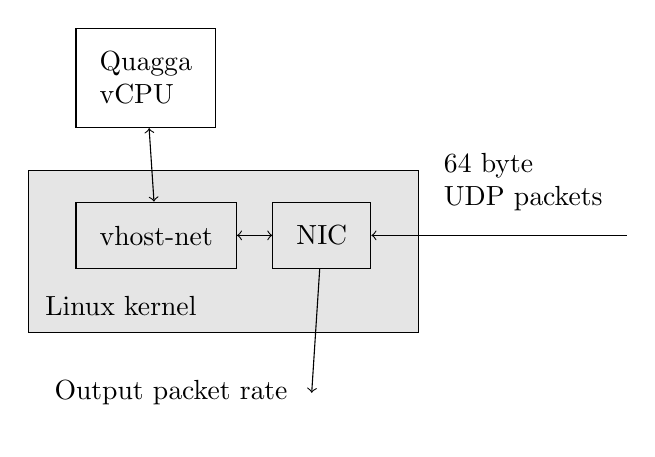
\begin{tikzpicture}
      \begin{scope}[rectangle, inner sep=0.3cm]
        \node[draw, anchor=west] (vhost) {vhost-net};
        \node[draw, anchor=west, align=left] (vm) at (0,2) {Quagga \\ vCPU};
        \node[draw, anchor=west] (nic) at (2.5,0) {NIC};
        \draw[<->] (vhost) to (vm);
        \draw[<->] (vhost) to (nic);
        \draw[<-] (nic) to (7,0) node[above left, align=left] {64 byte \\ UDP packets};
        \draw[->] (nic) to (3,-2) node[left] {Output packet rate};
      \end{scope}

      \begin{scope}[on background layer]
        \node[fill=black!10, fit=(vhost) (nic), draw, rectangle, inner sep=0.6cm, yshift=-0.2cm] (kernel){};
        \node[above right=0.1cm] at (kernel.south west) {Linux kernel};
      \end{scope}
    \end{tikzpicture} 
  \end{center}
\end{frame}

\begin{frame}\frametitle{Limit vhost-net thread}
  \begin{center}
    %LaTeX with PSTricks extensions
%%Creator: inkscape 0.92.4
%%Please note this file requires PSTricks extensions
\psset{xunit=.95pt,yunit=.95pt,runit=.95pt}
\begin{pspicture}(299.39044622,214.89599513)
{
\newrgbcolor{curcolor}{0.13725491 0.12156863 0.1254902}
\pscustom[linewidth=0.45333333,linecolor=curcolor]
{
\newpath
\moveto(30.90534803,23.44134316)
\lineto(33.75734797,23.44134316)
}
}
{
\newrgbcolor{curcolor}{0.13725491 0.12156863 0.1254902}
\pscustom[linewidth=0.45333333,linecolor=curcolor]
{
\newpath
\moveto(296.18000885,23.44134316)
\lineto(293.32667558,23.44134316)
}
}
{
\newrgbcolor{curcolor}{0.13725491 0.12156863 0.1254902}
\pscustom[linestyle=none,fillstyle=solid,fillcolor=curcolor]
{
\newpath
\moveto(15.42,23.76800773)
\curveto(16.18799998,24.01334106)(16.8213333,24.41867438)(16.8213333,25.1960077)
\curveto(16.8213333,25.62667436)(16.51733331,26.07334101)(15.89199999,26.07334101)
\curveto(15.12400001,26.07334101)(14.76933335,25.41467436)(14.64266668,25.17867437)
\lineto(14.51600002,25.21334103)
\curveto(14.85466668,26.31867434)(15.60533333,26.58000767)(16.17199998,26.58000767)
\curveto(17.25999996,26.58000767)(17.48933329,25.78667435)(17.48933329,25.44000769)
\curveto(17.48933329,24.9840077)(17.25999996,24.62134105)(16.70266664,24.25867439)
\curveto(17.0573333,24.10667439)(17.77599995,23.8106744)(17.77599995,22.69734109)
\curveto(17.77599995,21.49734111)(16.7613333,20.75467446)(15.436,20.75467446)
\curveto(15.23466667,20.75467446)(14.50000002,20.7960078)(14.50000002,21.23467445)
\curveto(14.50000002,21.47200778)(14.69333335,21.53067445)(14.82933335,21.53067445)
\curveto(15.21733334,21.53067445)(15.53733333,21.05867446)(16.03599999,21.05867446)
\curveto(16.8213333,21.05867446)(17.16799996,21.72534111)(17.16799996,22.35867443)
\curveto(17.16799996,22.56934109)(17.06666663,23.19467441)(16.52666664,23.47334107)
\curveto(16.22133332,23.63334107)(16.01066665,23.67600773)(15.428,23.6586744)
\lineto(15.42,23.76800773)
}
}
{
\newrgbcolor{curcolor}{0.13725491 0.12156863 0.1254902}
\pscustom[linestyle=none,fillstyle=solid,fillcolor=curcolor]
{
\newpath
\moveto(19.37334047,23.66800143)
\curveto(19.37334047,22.98266811)(19.39067381,20.97333482)(20.47067378,20.97333482)
\curveto(21.55200709,20.97333482)(21.56934042,23.00000145)(21.56934042,23.66800143)
\curveto(21.56934042,24.24133475)(21.55200709,26.36133471)(20.47067378,26.36133471)
\curveto(19.39067381,26.36133471)(19.37334047,24.24133475)(19.37334047,23.66800143)
\closepath
\moveto(22.38000707,23.66800143)
\curveto(22.38000707,22.64533479)(22.02534041,20.75466816)(20.47067378,20.75466816)
\curveto(18.91734048,20.75466816)(18.56267382,22.64533479)(18.56267382,23.66800143)
\curveto(18.56267382,24.66400141)(18.91734048,26.58000137)(20.47067378,26.58000137)
\curveto(22.02534041,26.58000137)(22.38000707,24.66400141)(22.38000707,23.66800143)
}
}
{
\newrgbcolor{curcolor}{0.13725491 0.12156863 0.1254902}
\pscustom[linestyle=none,fillstyle=solid,fillcolor=curcolor]
{
\newpath
\moveto(23.59732913,23.66800143)
\curveto(23.59732913,22.98266811)(23.61332913,20.97333482)(24.69466244,20.97333482)
\curveto(25.77599575,20.97333482)(25.79332909,23.00000145)(25.79332909,23.66800143)
\curveto(25.79332909,24.24133475)(25.77599575,26.36133471)(24.69466244,26.36133471)
\curveto(23.61332913,26.36133471)(23.59732913,24.24133475)(23.59732913,23.66800143)
\closepath
\moveto(26.6026624,23.66800143)
\curveto(26.6026624,22.64533479)(26.24799574,20.75466816)(24.69466244,20.75466816)
\curveto(23.14132914,20.75466816)(22.78666249,22.64533479)(22.78666249,23.66800143)
\curveto(22.78666249,24.66400141)(23.14132914,26.58000137)(24.69466244,26.58000137)
\curveto(26.24799574,26.58000137)(26.6026624,24.66400141)(26.6026624,23.66800143)
}
}
{
\newrgbcolor{curcolor}{0.13725491 0.12156863 0.1254902}
\pscustom[linewidth=0.45333333,linecolor=curcolor]
{
\newpath
\moveto(30.90534803,54.81731797)
\lineto(33.75734797,54.81731797)
}
}
{
\newrgbcolor{curcolor}{0.13725491 0.12156863 0.1254902}
\pscustom[linewidth=0.45333333,linecolor=curcolor]
{
\newpath
\moveto(296.18000885,54.81731797)
\lineto(293.32667558,54.81731797)
}
}
{
\newrgbcolor{curcolor}{0.13725491 0.12156863 0.1254902}
\pscustom[linestyle=none,fillstyle=solid,fillcolor=curcolor]
{
\newpath
\moveto(16.60134047,57.08000773)
\lineto(16.58534047,57.08000773)
\lineto(14.57467385,54.20934113)
\lineto(16.60134047,54.20934113)
\closepath
\moveto(18.12134044,53.66934114)
\lineto(17.26000712,53.66934114)
\lineto(17.26000712,52.2586745)
\lineto(16.60934047,52.2586745)
\lineto(16.60934047,53.66934114)
\lineto(14.23734052,53.66934114)
\lineto(14.23734052,54.20934113)
\lineto(16.88934047,57.96667438)
\lineto(17.26000712,57.96667438)
\lineto(17.26000712,54.20934113)
\lineto(18.12134044,54.20934113)
\lineto(18.12134044,53.66934114)
}
}
{
\newrgbcolor{curcolor}{0.13725491 0.12156863 0.1254902}
\pscustom[linestyle=none,fillstyle=solid,fillcolor=curcolor]
{
\newpath
\moveto(19.37334047,55.05331167)
\curveto(19.37334047,54.36931168)(19.39067381,52.35997839)(20.47067378,52.35997839)
\curveto(21.55200709,52.35997839)(21.56934042,54.38664502)(21.56934042,55.05331167)
\curveto(21.56934042,55.62797832)(21.55200709,57.74797828)(20.47067378,57.74797828)
\curveto(19.39067381,57.74797828)(19.37334047,55.62797832)(19.37334047,55.05331167)
\closepath
\moveto(22.38000707,55.05331167)
\curveto(22.38000707,54.03197836)(22.02534041,52.1399784)(20.47067378,52.1399784)
\curveto(18.91734048,52.1399784)(18.56267382,54.03197836)(18.56267382,55.05331167)
\curveto(18.56267382,56.04931165)(18.91734048,57.96664494)(20.47067378,57.96664494)
\curveto(22.02534041,57.96664494)(22.38000707,56.04931165)(22.38000707,55.05331167)
}
}
{
\newrgbcolor{curcolor}{0.13725491 0.12156863 0.1254902}
\pscustom[linestyle=none,fillstyle=solid,fillcolor=curcolor]
{
\newpath
\moveto(23.59732913,55.05331167)
\curveto(23.59732913,54.36931168)(23.61332913,52.35997839)(24.69466244,52.35997839)
\curveto(25.77599575,52.35997839)(25.79332909,54.38664502)(25.79332909,55.05331167)
\curveto(25.79332909,55.62797832)(25.77599575,57.74797828)(24.69466244,57.74797828)
\curveto(23.61332913,57.74797828)(23.59732913,55.62797832)(23.59732913,55.05331167)
\closepath
\moveto(26.6026624,55.05331167)
\curveto(26.6026624,54.03197836)(26.24799574,52.1399784)(24.69466244,52.1399784)
\curveto(23.14132914,52.1399784)(22.78666249,54.03197836)(22.78666249,55.05331167)
\curveto(22.78666249,56.04931165)(23.14132914,57.96664494)(24.69466244,57.96664494)
\curveto(26.24799574,57.96664494)(26.6026624,56.04931165)(26.6026624,55.05331167)
}
}
{
\newrgbcolor{curcolor}{0.13725491 0.12156863 0.1254902}
\pscustom[linewidth=0.45333333,linecolor=curcolor]
{
\newpath
\moveto(30.90534803,86.1946534)
\lineto(33.75734797,86.1946534)
}
}
{
\newrgbcolor{curcolor}{0.13725491 0.12156863 0.1254902}
\pscustom[linewidth=0.45333333,linecolor=curcolor]
{
\newpath
\moveto(296.18000885,86.1946534)
\lineto(293.32667558,86.1946534)
}
}
{
\newrgbcolor{curcolor}{0.13725491 0.12156863 0.1254902}
\pscustom[linestyle=none,fillstyle=solid,fillcolor=curcolor]
{
\newpath
\moveto(15.30933921,87.84933057)
\curveto(15.9853392,87.7306639)(16.77867251,87.58799724)(17.27733917,86.97999725)
\curveto(17.64000583,86.53999726)(17.73333916,86.29466393)(17.73333916,85.54399728)
\curveto(17.73333916,84.42133064)(16.80400585,83.52533066)(15.46933921,83.52533066)
\curveto(14.80267256,83.52533066)(14.40533923,83.72933066)(14.40533923,84.03199732)
\curveto(14.40533923,84.11733065)(14.40533923,84.36133064)(14.74400589,84.36133064)
\curveto(15.28400588,84.36133064)(15.51200587,83.83733065)(15.96800586,83.83733065)
\curveto(16.51600585,83.83733065)(17.14133917,84.31066398)(17.14133917,85.34133062)
\curveto(17.14133917,86.69333059)(15.64667254,87.08933058)(14.73467256,87.12399725)
\curveto(14.68400589,87.12399725)(14.65867256,87.17466391)(14.68400589,87.23333058)
\lineto(15.60533921,89.23466387)
\lineto(17.36933917,89.23466387)
\curveto(17.58933916,89.23466387)(17.66533916,89.32666387)(17.75867249,89.45466386)
\lineto(17.83467249,89.39466386)
\lineto(17.51333916,88.64266388)
\curveto(17.48800583,88.56666388)(17.41200583,88.56666388)(17.3186725,88.56666388)
\lineto(15.66400587,88.56666388)
\lineto(15.30933921,87.84933057)
}
}
{
\newrgbcolor{curcolor}{0.13725491 0.12156863 0.1254902}
\pscustom[linestyle=none,fillstyle=solid,fillcolor=curcolor]
{
\newpath
\moveto(19.37334047,86.4386597)
\curveto(19.37334047,85.75465971)(19.39067381,83.74532643)(20.47067378,83.74532643)
\curveto(21.55200709,83.74532643)(21.56934042,85.77199305)(21.56934042,86.4386597)
\curveto(21.56934042,87.01332635)(21.55200709,89.13332631)(20.47067378,89.13332631)
\curveto(19.39067381,89.13332631)(19.37334047,87.01332635)(19.37334047,86.4386597)
\closepath
\moveto(22.38000707,86.4386597)
\curveto(22.38000707,85.41599306)(22.02534041,83.52532643)(20.47067378,83.52532643)
\curveto(18.91734048,83.52532643)(18.56267382,85.41599306)(18.56267382,86.4386597)
\curveto(18.56267382,87.43465968)(18.91734048,89.35199297)(20.47067378,89.35199297)
\curveto(22.02534041,89.35199297)(22.38000707,87.43465968)(22.38000707,86.4386597)
}
}
{
\newrgbcolor{curcolor}{0.13725491 0.12156863 0.1254902}
\pscustom[linestyle=none,fillstyle=solid,fillcolor=curcolor]
{
\newpath
\moveto(23.59732913,86.4386597)
\curveto(23.59732913,85.75465971)(23.61332913,83.74532643)(24.69466244,83.74532643)
\curveto(25.77599575,83.74532643)(25.79332909,85.77199305)(25.79332909,86.4386597)
\curveto(25.79332909,87.01332635)(25.77599575,89.13332631)(24.69466244,89.13332631)
\curveto(23.61332913,89.13332631)(23.59732913,87.01332635)(23.59732913,86.4386597)
\closepath
\moveto(26.6026624,86.4386597)
\curveto(26.6026624,85.41599306)(26.24799574,83.52532643)(24.69466244,83.52532643)
\curveto(23.14132914,83.52532643)(22.78666249,85.41599306)(22.78666249,86.4386597)
\curveto(22.78666249,87.43465968)(23.14132914,89.35199297)(24.69466244,89.35199297)
\curveto(26.24799574,89.35199297)(26.6026624,87.43465968)(26.6026624,86.4386597)
}
}
{
\newrgbcolor{curcolor}{0.13725491 0.12156863 0.1254902}
\pscustom[linewidth=0.45333333,linecolor=curcolor]
{
\newpath
\moveto(30.90534803,117.570666)
\lineto(33.75734797,117.570666)
}
}
{
\newrgbcolor{curcolor}{0.13725491 0.12156863 0.1254902}
\pscustom[linewidth=0.45333333,linecolor=curcolor]
{
\newpath
\moveto(296.18000885,117.570666)
\lineto(293.32667558,117.570666)
}
}
{
\newrgbcolor{curcolor}{0.13725491 0.12156863 0.1254902}
\pscustom[linestyle=none,fillstyle=solid,fillcolor=curcolor]
{
\newpath
\moveto(15.37599874,117.98531797)
\curveto(15.29199874,117.90131797)(15.20799874,117.69865131)(15.20799874,117.19198465)
\curveto(15.20799874,115.77331802)(15.77333206,115.1479847)(16.40666538,115.1479847)
\curveto(16.93866537,115.1479847)(17.32666536,115.58798469)(17.32666536,116.541318)
\curveto(17.32666536,117.41065131)(17.07333204,118.25598463)(16.17866539,118.25598463)
\curveto(15.89199873,118.25598463)(15.5866654,118.18798463)(15.37599874,117.98531797)
\closepath
\moveto(17.91866535,120.67065124)
\curveto(16.41466538,120.43465125)(15.5786654,119.29465127)(15.41866541,118.26531796)
\curveto(15.8826654,118.54265129)(16.05999873,118.64398462)(16.53333205,118.64398462)
\curveto(17.42933203,118.64398462)(18.08666535,118.0026513)(18.08666535,116.87065133)
\curveto(18.08666535,116.25465134)(17.78266535,114.9119847)(16.27999872,114.9119847)
\curveto(15.28399874,114.9119847)(14.42266543,115.71465135)(14.42266543,117.48665131)
\curveto(14.42266543,119.20131794)(15.85733206,120.73865124)(17.90133202,120.80531791)
\lineto(17.91866535,120.67065124)
}
}
{
\newrgbcolor{curcolor}{0.13725491 0.12156863 0.1254902}
\pscustom[linestyle=none,fillstyle=solid,fillcolor=curcolor]
{
\newpath
\moveto(19.37334047,117.82533057)
\curveto(19.37334047,117.14133058)(19.39067381,115.13199729)(20.47067378,115.13199729)
\curveto(21.55200709,115.13199729)(21.56934042,117.15866391)(21.56934042,117.82533057)
\curveto(21.56934042,118.39999722)(21.55200709,120.51999717)(20.47067378,120.51999717)
\curveto(19.39067381,120.51999717)(19.37334047,118.39999722)(19.37334047,117.82533057)
\closepath
\moveto(22.38000707,117.82533057)
\curveto(22.38000707,116.80399725)(22.02534041,114.9119973)(20.47067378,114.9119973)
\curveto(18.91734048,114.9119973)(18.56267382,116.80399725)(18.56267382,117.82533057)
\curveto(18.56267382,118.82133054)(18.91734048,120.73866383)(20.47067378,120.73866383)
\curveto(22.02534041,120.73866383)(22.38000707,118.82133054)(22.38000707,117.82533057)
}
}
{
\newrgbcolor{curcolor}{0.13725491 0.12156863 0.1254902}
\pscustom[linestyle=none,fillstyle=solid,fillcolor=curcolor]
{
\newpath
\moveto(23.59732913,117.82533057)
\curveto(23.59732913,117.14133058)(23.61332913,115.13199729)(24.69466244,115.13199729)
\curveto(25.77599575,115.13199729)(25.79332909,117.15866391)(25.79332909,117.82533057)
\curveto(25.79332909,118.39999722)(25.77599575,120.51999717)(24.69466244,120.51999717)
\curveto(23.61332913,120.51999717)(23.59732913,118.39999722)(23.59732913,117.82533057)
\closepath
\moveto(26.6026624,117.82533057)
\curveto(26.6026624,116.80399725)(26.24799574,114.9119973)(24.69466244,114.9119973)
\curveto(23.14132914,114.9119973)(22.78666249,116.80399725)(22.78666249,117.82533057)
\curveto(22.78666249,118.82133054)(23.14132914,120.73866383)(24.69466244,120.73866383)
\curveto(26.24799574,120.73866383)(26.6026624,118.82133054)(26.6026624,117.82533057)
}
}
{
\newrgbcolor{curcolor}{0.13725491 0.12156863 0.1254902}
\pscustom[linewidth=0.45333333,linecolor=curcolor]
{
\newpath
\moveto(30.90534803,148.99199513)
\lineto(33.75734797,148.99199513)
}
}
{
\newrgbcolor{curcolor}{0.13725491 0.12156863 0.1254902}
\pscustom[linewidth=0.45333333,linecolor=curcolor]
{
\newpath
\moveto(296.18000885,148.99199513)
\lineto(293.32667558,148.99199513)
}
}
{
\newrgbcolor{curcolor}{0.13725491 0.12156863 0.1254902}
\pscustom[linestyle=none,fillstyle=solid,fillcolor=curcolor]
{
\newpath
\moveto(17.92666961,151.8706723)
\lineto(16.13733631,146.34800575)
\lineto(15.58800299,146.34800575)
\lineto(17.26000295,151.38000564)
\lineto(15.42800299,151.38000564)
\curveto(14.87866967,151.38000564)(14.72666968,151.13600565)(14.44800302,150.69733899)
\lineto(14.30533635,150.76400566)
\lineto(14.66800301,151.6346723)
\lineto(14.80266968,152.00533896)
\lineto(17.92666961,152.00533896)
\lineto(17.92666961,151.8706723)
}
}
{
\newrgbcolor{curcolor}{0.13725491 0.12156863 0.1254902}
\pscustom[linestyle=none,fillstyle=solid,fillcolor=curcolor]
{
\newpath
\moveto(19.37334047,149.2106408)
\curveto(19.37334047,148.52664082)(19.39067381,146.51597419)(20.47067378,146.51597419)
\curveto(21.55200709,146.51597419)(21.56934042,148.54264082)(21.56934042,149.2106408)
\curveto(21.56934042,149.78530746)(21.55200709,151.90397408)(20.47067378,151.90397408)
\curveto(19.39067381,151.90397408)(19.37334047,149.78530746)(19.37334047,149.2106408)
\closepath
\moveto(22.38000707,149.2106408)
\curveto(22.38000707,148.18930749)(22.02534041,146.29730753)(20.47067378,146.29730753)
\curveto(18.91734048,146.29730753)(18.56267382,148.18930749)(18.56267382,149.2106408)
\curveto(18.56267382,150.20664078)(18.91734048,152.12397407)(20.47067378,152.12397407)
\curveto(22.02534041,152.12397407)(22.38000707,150.20664078)(22.38000707,149.2106408)
}
}
{
\newrgbcolor{curcolor}{0.13725491 0.12156863 0.1254902}
\pscustom[linestyle=none,fillstyle=solid,fillcolor=curcolor]
{
\newpath
\moveto(23.59732913,149.2106408)
\curveto(23.59732913,148.52664082)(23.61332913,146.51597419)(24.69466244,146.51597419)
\curveto(25.77599575,146.51597419)(25.79332909,148.54264082)(25.79332909,149.2106408)
\curveto(25.79332909,149.78530746)(25.77599575,151.90397408)(24.69466244,151.90397408)
\curveto(23.61332913,151.90397408)(23.59732913,149.78530746)(23.59732913,149.2106408)
\closepath
\moveto(26.6026624,149.2106408)
\curveto(26.6026624,148.18930749)(26.24799574,146.29730753)(24.69466244,146.29730753)
\curveto(23.14132914,146.29730753)(22.78666249,148.18930749)(22.78666249,149.2106408)
\curveto(22.78666249,150.20664078)(23.14132914,152.12397407)(24.69466244,152.12397407)
\curveto(26.24799574,152.12397407)(26.6026624,150.20664078)(26.6026624,149.2106408)
}
}
{
\newrgbcolor{curcolor}{0.13725491 0.12156863 0.1254902}
\pscustom[linewidth=0.45333333,linecolor=curcolor]
{
\newpath
\moveto(30.90534803,180.36933057)
\lineto(33.75734797,180.36933057)
}
}
{
\newrgbcolor{curcolor}{0.13725491 0.12156863 0.1254902}
\pscustom[linewidth=0.45333333,linecolor=curcolor]
{
\newpath
\moveto(296.18000885,180.36933057)
\lineto(293.32667558,180.36933057)
}
}
{
\newrgbcolor{curcolor}{0.13725491 0.12156863 0.1254902}
\pscustom[linestyle=none,fillstyle=solid,fillcolor=curcolor]
{
\newpath
\moveto(16.34000126,181.0866471)
\curveto(16.66133459,181.29731376)(17.13466791,181.61064709)(17.13466791,182.35331374)
\curveto(17.13466791,182.81731373)(16.83866792,183.27331372)(16.18800126,183.27331372)
\curveto(15.55466794,183.27331372)(15.28400128,182.82664706)(15.28400128,182.42131374)
\curveto(15.28400128,181.76264709)(16.03600127,181.28131376)(16.34000126,181.0866471)
\closepath
\moveto(15.25066795,179.11864714)
\curveto(15.25066795,178.46931383)(15.64000128,177.9199805)(16.32266793,177.9199805)
\curveto(16.85600125,177.9199805)(17.25200124,178.27464716)(17.25200124,178.86531382)
\curveto(17.25200124,179.49064714)(16.89733458,179.74398046)(15.92666794,180.43731378)
\curveto(15.65600127,180.21731379)(15.25066795,179.88798046)(15.25066795,179.11864714)
\closepath
\moveto(15.70666794,180.60531378)
\curveto(14.99733462,181.22931376)(14.6600013,181.51731376)(14.6600013,182.20131374)
\curveto(14.6600013,183.05464706)(15.51200128,183.51064705)(16.23866793,183.51064705)
\curveto(17.19333457,183.51064705)(17.71600123,182.95331373)(17.71600123,182.31064707)
\curveto(17.71600123,181.53331376)(17.04133458,181.17998043)(16.58533459,180.9346471)
\curveto(17.71600123,180.12398046)(17.89333456,179.63464713)(17.89333456,179.06798048)
\curveto(17.89333456,178.62931382)(17.6146679,177.68398051)(16.2133346,177.68398051)
\curveto(15.16666795,177.68398051)(14.60933463,178.37598049)(14.60933463,179.03464715)
\curveto(14.60933463,179.7693138)(14.95466796,180.03064712)(15.70666794,180.60531378)
}
}
{
\newrgbcolor{curcolor}{0.13725491 0.12156863 0.1254902}
\pscustom[linestyle=none,fillstyle=solid,fillcolor=curcolor]
{
\newpath
\moveto(19.37334047,180.59598883)
\curveto(19.37334047,179.91198885)(19.39067381,177.90265556)(20.47067378,177.90265556)
\curveto(21.55200709,177.90265556)(21.56934042,179.92932218)(21.56934042,180.59598883)
\curveto(21.56934042,181.17065549)(21.55200709,183.29065544)(20.47067378,183.29065544)
\curveto(19.39067381,183.29065544)(19.37334047,181.17065549)(19.37334047,180.59598883)
\closepath
\moveto(22.38000707,180.59598883)
\curveto(22.38000707,179.57332219)(22.02534041,177.68265556)(20.47067378,177.68265556)
\curveto(18.91734048,177.68265556)(18.56267382,179.57332219)(18.56267382,180.59598883)
\curveto(18.56267382,181.59198881)(18.91734048,183.5093221)(20.47067378,183.5093221)
\curveto(22.02534041,183.5093221)(22.38000707,181.59198881)(22.38000707,180.59598883)
}
}
{
\newrgbcolor{curcolor}{0.13725491 0.12156863 0.1254902}
\pscustom[linestyle=none,fillstyle=solid,fillcolor=curcolor]
{
\newpath
\moveto(23.59732913,180.59598883)
\curveto(23.59732913,179.91198885)(23.61332913,177.90265556)(24.69466244,177.90265556)
\curveto(25.77599575,177.90265556)(25.79332909,179.92932218)(25.79332909,180.59598883)
\curveto(25.79332909,181.17065549)(25.77599575,183.29065544)(24.69466244,183.29065544)
\curveto(23.61332913,183.29065544)(23.59732913,181.17065549)(23.59732913,180.59598883)
\closepath
\moveto(26.6026624,180.59598883)
\curveto(26.6026624,179.57332219)(26.24799574,177.68265556)(24.69466244,177.68265556)
\curveto(23.14132914,177.68265556)(22.78666249,179.57332219)(22.78666249,180.59598883)
\curveto(22.78666249,181.59198881)(23.14132914,183.5093221)(24.69466244,183.5093221)
\curveto(26.24799574,183.5093221)(26.6026624,181.59198881)(26.6026624,180.59598883)
}
}
{
\newrgbcolor{curcolor}{0.13725491 0.12156863 0.1254902}
\pscustom[linewidth=0.45333333,linecolor=curcolor]
{
\newpath
\moveto(30.90534803,211.746666)
\lineto(33.75734797,211.746666)
}
}
{
\newrgbcolor{curcolor}{0.13725491 0.12156863 0.1254902}
\pscustom[linewidth=0.45333333,linecolor=curcolor]
{
\newpath
\moveto(296.18000885,211.746666)
\lineto(293.32667558,211.746666)
}
}
{
\newrgbcolor{curcolor}{0.13725491 0.12156863 0.1254902}
\pscustom[linestyle=none,fillstyle=solid,fillcolor=curcolor]
{
\newpath
\moveto(17.19200126,212.514666)
\curveto(17.19200126,213.01333265)(17.19200126,214.65866595)(16.06933462,214.65866595)
\curveto(15.3600013,214.65866595)(15.16533464,213.87466597)(15.16533464,213.18133265)
\curveto(15.16533464,212.53999933)(15.3520013,211.55199935)(16.24666795,211.55199935)
\curveto(16.52533461,211.55199935)(16.88000127,211.70399935)(17.0573346,211.84799935)
\curveto(17.16666793,211.93199934)(17.19200126,212.03333268)(17.19200126,212.18533267)
\closepath
\moveto(14.60933465,209.17066607)
\curveto(16.65200127,209.50933273)(17.11600126,211.42666602)(17.16666793,211.63733268)
\lineto(17.14933459,211.65333268)
\curveto(16.77866794,211.34133269)(16.33066795,211.18933269)(15.90933462,211.18933269)
\curveto(14.77733465,211.18933269)(14.38933465,212.16799934)(14.38933465,212.86133266)
\curveto(14.38933465,213.9839993)(15.06400131,214.89599928)(16.16133462,214.89599928)
\curveto(17.20000126,214.89599928)(18.01066791,213.94133263)(18.01066791,212.53199933)
\curveto(18.01066791,210.7413327)(16.77866794,209.13733274)(14.63466798,209.00266608)
\lineto(14.60933465,209.17066607)
}
}
{
\newrgbcolor{curcolor}{0.13725491 0.12156863 0.1254902}
\pscustom[linestyle=none,fillstyle=solid,fillcolor=curcolor]
{
\newpath
\moveto(19.37334047,211.9826597)
\curveto(19.37334047,211.29865971)(19.39067381,209.28799309)(20.47067378,209.28799309)
\curveto(21.55200709,209.28799309)(21.56934042,211.31599305)(21.56934042,211.9826597)
\curveto(21.56934042,212.55732635)(21.55200709,214.67732631)(20.47067378,214.67732631)
\curveto(19.39067381,214.67732631)(19.37334047,212.55732635)(19.37334047,211.9826597)
\closepath
\moveto(22.38000707,211.9826597)
\curveto(22.38000707,210.96132639)(22.02534041,209.06932643)(20.47067378,209.06932643)
\curveto(18.91734048,209.06932643)(18.56267382,210.96132639)(18.56267382,211.9826597)
\curveto(18.56267382,212.97865968)(18.91734048,214.89599297)(20.47067378,214.89599297)
\curveto(22.02534041,214.89599297)(22.38000707,212.97865968)(22.38000707,211.9826597)
}
}
{
\newrgbcolor{curcolor}{0.13725491 0.12156863 0.1254902}
\pscustom[linestyle=none,fillstyle=solid,fillcolor=curcolor]
{
\newpath
\moveto(23.59732913,211.9826597)
\curveto(23.59732913,211.29865971)(23.61332913,209.28799309)(24.69466244,209.28799309)
\curveto(25.77599575,209.28799309)(25.79332909,211.31599305)(25.79332909,211.9826597)
\curveto(25.79332909,212.55732635)(25.77599575,214.67732631)(24.69466244,214.67732631)
\curveto(23.61332913,214.67732631)(23.59732913,212.55732635)(23.59732913,211.9826597)
\closepath
\moveto(26.6026624,211.9826597)
\curveto(26.6026624,210.96132639)(26.24799574,209.06932643)(24.69466244,209.06932643)
\curveto(23.14132914,209.06932643)(22.78666249,210.96132639)(22.78666249,211.9826597)
\curveto(22.78666249,212.97865968)(23.14132914,214.89599297)(24.69466244,214.89599297)
\curveto(26.24799574,214.89599297)(26.6026624,212.97865968)(26.6026624,211.9826597)
}
}
{
\newrgbcolor{curcolor}{0.13725491 0.12156863 0.1254902}
\pscustom[linewidth=0.45333333,linecolor=curcolor]
{
\newpath
\moveto(57.43732913,23.44134316)
\lineto(57.43732913,26.2933431)
}
}
{
\newrgbcolor{curcolor}{0.13725491 0.12156863 0.1254902}
\pscustom[linewidth=0.45333333,linecolor=curcolor]
{
\newpath
\moveto(57.43732913,211.74667235)
\lineto(57.43732913,208.89333908)
}
}
{
\newrgbcolor{curcolor}{0.13725491 0.12156863 0.1254902}
\pscustom[linestyle=none,fillstyle=solid,fillcolor=curcolor]
{
\newpath
\moveto(54.41332913,17.83732427)
\curveto(55.08932912,17.7186576)(55.88266243,17.57465761)(56.37999576,16.96665762)
\curveto(56.74399575,16.52799096)(56.83599575,16.28265763)(56.83599575,15.53199098)
\curveto(56.83599575,14.40799101)(55.90799577,13.51332436)(54.57332913,13.51332436)
\curveto(53.90666248,13.51332436)(53.50932915,13.71599102)(53.50932915,14.01999102)
\curveto(53.50932915,14.10399102)(53.50932915,14.34932434)(53.84666248,14.34932434)
\curveto(54.38666247,14.34932434)(54.6159958,13.82532435)(55.07199579,13.82532435)
\curveto(55.61999577,13.82532435)(56.24532909,14.29865768)(56.24532909,15.32932432)
\curveto(56.24532909,16.67999096)(54.75066246,17.07732428)(53.83866248,17.11065762)
\curveto(53.78799581,17.11065762)(53.76266248,17.16132428)(53.78799581,17.22132428)
\lineto(54.70932913,19.22132424)
\lineto(56.47332909,19.22132424)
\curveto(56.69332908,19.22132424)(56.76932908,19.31465757)(56.86132908,19.44132423)
\lineto(56.93732908,19.38265757)
\lineto(56.61732909,18.63065758)
\curveto(56.59199575,18.55465758)(56.51599575,18.55465758)(56.42266242,18.55465758)
\lineto(54.76799579,18.55465758)
\lineto(54.41332913,17.83732427)
}
}
{
\newrgbcolor{curcolor}{0.13725491 0.12156863 0.1254902}
\pscustom[linestyle=none,fillstyle=solid,fillcolor=curcolor]
{
\newpath
\moveto(58.47734173,16.4266534)
\curveto(58.47734173,15.74265342)(58.49467507,13.73198679)(59.57467504,13.73198679)
\curveto(60.65600835,13.73198679)(60.67200835,15.75998675)(60.67200835,16.4266534)
\curveto(60.67200835,17.00132005)(60.65600835,19.11998667)(59.57467504,19.11998667)
\curveto(58.49467507,19.11998667)(58.47734173,17.00132005)(58.47734173,16.4266534)
\closepath
\moveto(61.482675,16.4266534)
\curveto(61.482675,15.40532009)(61.12934167,13.51332013)(59.57467504,13.51332013)
\curveto(58.02134174,13.51332013)(57.66667508,15.40532009)(57.66667508,16.4266534)
\curveto(57.66667508,17.42265338)(58.02134174,19.33998667)(59.57467504,19.33998667)
\curveto(61.12934167,19.33998667)(61.482675,17.42265338)(61.482675,16.4266534)
}
}
{
\newrgbcolor{curcolor}{0.13725491 0.12156863 0.1254902}
\pscustom[linewidth=0.45333333,linecolor=curcolor]
{
\newpath
\moveto(110.50132913,23.44134316)
\lineto(110.50132913,26.2933431)
}
}
{
\newrgbcolor{curcolor}{0.13725491 0.12156863 0.1254902}
\pscustom[linewidth=0.45333333,linecolor=curcolor]
{
\newpath
\moveto(110.50132913,211.74667235)
\lineto(110.50132913,208.89333908)
}
}
{
\newrgbcolor{curcolor}{0.13725491 0.12156863 0.1254902}
\pscustom[linestyle=none,fillstyle=solid,fillcolor=curcolor]
{
\newpath
\moveto(107.5280126,16.5866786)
\curveto(107.4440126,16.5026786)(107.3600126,16.30001194)(107.3600126,15.79334528)
\curveto(107.3600126,14.37467865)(107.92534592,13.74934533)(108.55867924,13.74934533)
\curveto(109.0893459,13.74934533)(109.47867922,14.18934532)(109.47867922,15.14267863)
\curveto(109.47867922,16.01201194)(109.22534589,16.85734526)(108.33067925,16.85734526)
\curveto(108.04267925,16.85734526)(107.73867926,16.78934526)(107.5280126,16.5866786)
\closepath
\moveto(110.06934588,19.27201187)
\curveto(108.56667924,19.03601188)(107.73067926,17.8960119)(107.57067926,16.86667859)
\curveto(108.03467925,17.14401192)(108.21201258,17.24534525)(108.68534591,17.24534525)
\curveto(109.58001255,17.24534525)(110.23867921,16.60401193)(110.23867921,15.47201196)
\curveto(110.23867921,14.85601197)(109.93467921,13.51334533)(108.43067925,13.51334533)
\curveto(107.43467927,13.51334533)(106.57467929,14.31601198)(106.57467929,16.08934527)
\curveto(106.57467929,17.80267857)(108.00934592,19.34001187)(110.05201254,19.40667853)
\lineto(110.06934588,19.27201187)
}
}
{
\newrgbcolor{curcolor}{0.13725491 0.12156863 0.1254902}
\pscustom[linestyle=none,fillstyle=solid,fillcolor=curcolor]
{
\newpath
\moveto(111.52531654,16.4266534)
\curveto(111.52531654,15.74265342)(111.54131654,13.73198679)(112.62264984,13.73198679)
\curveto(113.70398315,13.73198679)(113.71998315,15.75998675)(113.71998315,16.4266534)
\curveto(113.71998315,17.00132005)(113.70398315,19.11998667)(112.62264984,19.11998667)
\curveto(111.54131654,19.11998667)(111.52531654,17.00132005)(111.52531654,16.4266534)
\closepath
\moveto(114.5306498,16.4266534)
\curveto(114.5306498,15.40532009)(114.17598314,13.51332013)(112.62264984,13.51332013)
\curveto(111.06931655,13.51332013)(110.71464989,15.40532009)(110.71464989,16.4266534)
\curveto(110.71464989,17.42265338)(111.06931655,19.33998667)(112.62264984,19.33998667)
\curveto(114.17598314,19.33998667)(114.5306498,17.42265338)(114.5306498,16.4266534)
}
}
{
\newrgbcolor{curcolor}{0.13725491 0.12156863 0.1254902}
\pscustom[linewidth=0.45333333,linecolor=curcolor]
{
\newpath
\moveto(163.56532913,23.44134316)
\lineto(163.56532913,26.2933431)
}
}
{
\newrgbcolor{curcolor}{0.13725491 0.12156863 0.1254902}
\pscustom[linewidth=0.45333333,linecolor=curcolor]
{
\newpath
\moveto(163.56532913,211.74667235)
\lineto(163.56532913,208.89333908)
}
}
{
\newrgbcolor{curcolor}{0.13725491 0.12156863 0.1254902}
\pscustom[linestyle=none,fillstyle=solid,fillcolor=curcolor]
{
\newpath
\moveto(163.12531654,19.0866849)
\lineto(161.33464991,13.56401835)
\lineto(160.78664992,13.56401835)
\lineto(162.45864988,18.59601824)
\lineto(160.62664992,18.59601824)
\curveto(160.0773166,18.59601824)(159.92664994,18.35201825)(159.64664995,17.91335159)
\lineto(159.50264995,17.98135159)
\lineto(159.86664994,18.8506849)
\lineto(160.0013166,19.22135156)
\lineto(163.12531654,19.22135156)
\lineto(163.12531654,19.0866849)
}
}
{
\newrgbcolor{curcolor}{0.13725491 0.12156863 0.1254902}
\pscustom[linestyle=none,fillstyle=solid,fillcolor=curcolor]
{
\newpath
\moveto(164.5720063,16.4266534)
\curveto(164.5720063,15.74265342)(164.58933963,13.73198679)(165.66933961,13.73198679)
\curveto(166.75067292,13.73198679)(166.76667292,15.75998675)(166.76667292,16.4266534)
\curveto(166.76667292,17.00132005)(166.75067292,19.11998667)(165.66933961,19.11998667)
\curveto(164.58933963,19.11998667)(164.5720063,17.00132005)(164.5720063,16.4266534)
\closepath
\moveto(167.5786729,16.4266534)
\curveto(167.5786729,15.40532009)(167.22267291,13.51332013)(165.66933961,13.51332013)
\curveto(164.11600631,13.51332013)(163.76000632,15.40532009)(163.76000632,16.4266534)
\curveto(163.76000632,17.42265338)(164.11600631,19.33998667)(165.66933961,19.33998667)
\curveto(167.22267291,19.33998667)(167.5786729,17.42265338)(167.5786729,16.4266534)
}
}
{
\newrgbcolor{curcolor}{0.13725491 0.12156863 0.1254902}
\pscustom[linewidth=0.45333333,linecolor=curcolor]
{
\newpath
\moveto(216.5840126,23.44134316)
\lineto(216.5840126,26.2933431)
}
}
{
\newrgbcolor{curcolor}{0.13725491 0.12156863 0.1254902}
\pscustom[linewidth=0.45333333,linecolor=curcolor]
{
\newpath
\moveto(216.5840126,211.74667235)
\lineto(216.5840126,208.89333908)
}
}
{
\newrgbcolor{curcolor}{0.13725491 0.12156863 0.1254902}
\pscustom[linestyle=none,fillstyle=solid,fillcolor=curcolor]
{
\newpath
\moveto(214.5880063,16.91598883)
\curveto(214.90667296,17.1266555)(215.37867295,17.43998882)(215.37867295,18.18265547)
\curveto(215.37867295,18.6479888)(215.08533962,19.10265545)(214.4320063,19.10265545)
\curveto(213.80133965,19.10265545)(213.53200632,18.65598879)(213.53200632,18.25065547)
\curveto(213.53200632,17.59198882)(214.28133964,17.1106555)(214.5880063,16.91598883)
\closepath
\moveto(213.49733966,14.94932221)
\curveto(213.49733966,14.29865556)(213.88533965,13.74932224)(214.5680063,13.74932224)
\curveto(215.10133962,13.74932224)(215.49733961,14.1039889)(215.49733961,14.69598888)
\curveto(215.49733961,15.31998887)(215.14267295,15.5733222)(214.17200631,16.26665551)
\curveto(213.90267298,16.04665552)(213.49733966,15.71732219)(213.49733966,14.94932221)
\closepath
\moveto(213.95200631,16.43465551)
\curveto(213.242673,17.05998883)(212.906673,17.34665549)(212.906673,18.03198881)
\curveto(212.906673,18.88398879)(213.76000632,19.33998878)(214.48533963,19.33998878)
\curveto(215.44000628,19.33998878)(215.96267294,18.78265546)(215.96267294,18.14132214)
\curveto(215.96267294,17.36398882)(215.28533962,17.00932216)(214.83200629,16.76398884)
\curveto(215.96267294,15.95332219)(216.1413396,15.46398887)(216.1413396,14.89865554)
\curveto(216.1413396,14.45865555)(215.8613396,13.51332224)(214.46133964,13.51332224)
\curveto(213.41333966,13.51332224)(212.854673,14.20532223)(212.854673,14.86398888)
\curveto(212.854673,15.59865553)(213.20133966,15.86132219)(213.95200631,16.43465551)
}
}
{
\newrgbcolor{curcolor}{0.13725491 0.12156863 0.1254902}
\pscustom[linestyle=none,fillstyle=solid,fillcolor=curcolor]
{
\newpath
\moveto(217.62134173,16.4266534)
\curveto(217.62134173,15.74265342)(217.63734173,13.73198679)(218.71734171,13.73198679)
\curveto(219.79867502,13.73198679)(219.81600835,15.75998675)(219.81600835,16.4266534)
\curveto(219.81600835,17.00132005)(219.79867502,19.11998667)(218.71734171,19.11998667)
\curveto(217.63734173,19.11998667)(217.62134173,17.00132005)(217.62134173,16.4266534)
\closepath
\moveto(220.626675,16.4266534)
\curveto(220.626675,15.40532009)(220.27200834,13.51332013)(218.71734171,13.51332013)
\curveto(217.16400841,13.51332013)(216.80934175,15.40532009)(216.80934175,16.4266534)
\curveto(216.80934175,17.42265338)(217.16400841,19.33998667)(218.71734171,19.33998667)
\curveto(220.27200834,19.33998667)(220.626675,17.42265338)(220.626675,16.4266534)
}
}
{
\newrgbcolor{curcolor}{0.13725491 0.12156863 0.1254902}
\pscustom[linewidth=0.45333333,linecolor=curcolor]
{
\newpath
\moveto(269.6480126,23.44134316)
\lineto(269.6480126,26.2933431)
}
}
{
\newrgbcolor{curcolor}{0.13725491 0.12156863 0.1254902}
\pscustom[linewidth=0.45333333,linecolor=curcolor]
{
\newpath
\moveto(269.6480126,211.74667235)
\lineto(269.6480126,208.89333908)
}
}
{
\newrgbcolor{curcolor}{0.13725491 0.12156863 0.1254902}
\pscustom[linestyle=none,fillstyle=solid,fillcolor=curcolor]
{
\newpath
\moveto(268.48667717,16.9586597)
\curveto(268.48667717,17.45599302)(268.48667717,19.10265965)(267.36401052,19.10265965)
\curveto(266.65334387,19.10265965)(266.46001054,18.31732634)(266.46001054,17.62532635)
\curveto(266.46001054,16.98399303)(266.64667721,15.99599305)(267.54001052,15.99599305)
\curveto(267.82001051,15.99599305)(268.17467717,16.14799305)(268.3520105,16.29199305)
\curveto(268.46134383,16.37599305)(268.48667717,16.47732638)(268.48667717,16.62932637)
\closepath
\moveto(265.90267722,13.61465977)
\curveto(267.94667718,13.95332643)(268.4120105,15.86932639)(268.46134383,16.08132639)
\lineto(268.4440105,16.09732639)
\curveto(268.07334384,15.78532639)(267.62667718,15.6333264)(267.20534386,15.6333264)
\curveto(266.07201055,15.6333264)(265.68267723,16.61199304)(265.68267723,17.30532636)
\curveto(265.68267723,18.427993)(266.35867721,19.33999298)(267.45734385,19.33999298)
\curveto(268.49467717,19.33999298)(269.30667715,18.38532633)(269.30667715,16.97599303)
\curveto(269.30667715,15.18532641)(268.07334384,13.58132644)(265.92667722,13.44665978)
\lineto(265.90267722,13.61465977)
}
}
{
\newrgbcolor{curcolor}{0.13725491 0.12156863 0.1254902}
\pscustom[linestyle=none,fillstyle=solid,fillcolor=curcolor]
{
\newpath
\moveto(270.6679937,16.4266534)
\curveto(270.6679937,15.74265342)(270.68532703,13.73198679)(271.76532701,13.73198679)
\curveto(272.84666032,13.73198679)(272.86266032,15.75998675)(272.86266032,16.4266534)
\curveto(272.86266032,17.00132005)(272.84666032,19.11998667)(271.76532701,19.11998667)
\curveto(270.68532703,19.11998667)(270.6679937,17.00132005)(270.6679937,16.4266534)
\closepath
\moveto(273.6746603,16.4266534)
\curveto(273.6746603,15.40532009)(273.31866031,13.51332013)(271.76532701,13.51332013)
\curveto(270.21066038,13.51332013)(269.85732705,15.40532009)(269.85732705,16.4266534)
\curveto(269.85732705,17.42265338)(270.21066038,19.33998667)(271.76532701,19.33998667)
\curveto(273.31866031,19.33998667)(273.6746603,17.42265338)(273.6746603,16.4266534)
}
}
{
\newrgbcolor{curcolor}{0.13725491 0.12156863 0.1254902}
\pscustom[linewidth=0.45333331,linecolor=curcolor]
{
\newpath
\moveto(30.90534803,23.44134316)
\lineto(296.1799937,23.44134316)
\lineto(296.1799937,211.746666)
\lineto(30.90534803,211.746666)
\closepath
}
}
{
\newrgbcolor{curcolor}{0.13725491 0.12156863 0.1254902}
\pscustom[linestyle=none,fillstyle=solid,fillcolor=curcolor]
{
\newpath
\moveto(3.47199874,75.44133057)
\curveto(1.22266546,75.44133057)(0.42399881,74.34666392)(0.42399881,73.34133061)
\curveto(0.42399881,72.33466397)(1.22266546,71.23999732)(3.47199874,71.23999732)
\curveto(5.64133203,71.23999732)(6.51866534,72.24666397)(6.51866534,73.34133061)
\curveto(6.51866534,74.43466392)(5.64133203,75.44133057)(3.47199874,75.44133057)
\closepath
\moveto(3.48266541,70.11599735)
\curveto(1.21333212,70.11599735)(0.06933215,71.72399731)(0.06933215,73.34133061)
\curveto(0.06933215,74.95733058)(1.21333212,76.56533054)(3.48266541,76.56533054)
\curveto(5.58266536,76.56533054)(6.87466533,75.12533057)(6.87466533,73.34133061)
\curveto(6.87466533,71.55599732)(5.58266536,70.11599735)(3.48266541,70.11599735)
}
}
{
\newrgbcolor{curcolor}{0.13725491 0.12156863 0.1254902}
\pscustom[linestyle=none,fillstyle=solid,fillcolor=curcolor]
{
\newpath
\moveto(6.38133921,81.63200773)
\curveto(6.51867254,81.09867441)(6.65733921,80.72400775)(6.8253392,80.26000776)
\lineto(6.8053392,80.24000776)
\lineto(5.98667255,80.24000776)
\lineto(6.41067255,79.81600777)
\curveto(6.79600587,79.43200778)(6.83467254,78.95867446)(6.83467254,78.78134113)
\curveto(6.83467254,78.3760078)(6.59867254,77.60667449)(5.55333923,77.60667449)
\lineto(3.06800595,77.60667449)
\curveto(2.47600597,77.60667449)(2.45600597,77.29067449)(2.43600597,76.99600783)
\lineto(2.29867264,76.99600783)
\lineto(2.29867264,78.4360078)
\lineto(5.51333923,78.4360078)
\curveto(5.6520059,78.4360078)(6.26267255,78.5240078)(6.26267255,79.17600779)
\curveto(6.26267255,79.47067445)(6.12533922,79.76667444)(5.90800589,80.0333411)
\curveto(5.82800589,80.1213411)(5.73067256,80.19067443)(5.40533923,80.19067443)
\lineto(3.08667262,80.19067443)
\curveto(2.69200596,80.19067443)(2.4853393,80.15200776)(2.4653393,79.46134111)
\lineto(2.29867264,79.46134111)
\lineto(2.29867264,81.02000774)
\lineto(5.68133923,81.02000774)
\curveto(6.03600589,81.02000774)(6.26267255,81.03867441)(6.24267255,81.63200773)
\lineto(6.38133921,81.63200773)
}
}
{
\newrgbcolor{curcolor}{0.13725491 0.12156863 0.1254902}
\pscustom[linestyle=none,fillstyle=solid,fillcolor=curcolor]
{
\newpath
\moveto(2.61333921,84.35731167)
\lineto(2.61333921,83.36131169)
\lineto(5.43467248,83.36131169)
\curveto(5.74000581,83.36131169)(6.32133913,83.36131169)(6.32133913,83.86397835)
\curveto(6.32133913,84.17864501)(6.10533914,84.35731167)(5.97600581,84.46531167)
\lineto(6.08533914,84.59331166)
\curveto(6.50933913,84.35731167)(6.83467245,83.89331168)(6.83467245,83.43997835)
\curveto(6.83467245,82.9373117)(6.56800579,82.53331171)(5.58267248,82.53331171)
\lineto(2.61333921,82.53331171)
\lineto(2.61333921,82.00931172)
\curveto(2.60400588,81.99064505)(2.57467255,81.97064505)(2.54400588,81.97064505)
\curveto(2.42667255,81.97064505)(2.36667255,82.18797838)(2.14933922,82.40531171)
\curveto(1.76533923,82.77997837)(1.5480059,82.92664503)(1.02533925,83.29197836)
\curveto(1.02533925,83.36131169)(1.07467258,83.36131169)(1.15333924,83.36131169)
\lineto(2.29733922,83.36131169)
\lineto(2.29733922,84.35731167)
\lineto(2.61333921,84.35731167)
}
}
{
\newrgbcolor{curcolor}{0.13725491 0.12156863 0.1254902}
\pscustom[linestyle=none,fillstyle=solid,fillcolor=curcolor]
{
\newpath
\moveto(5.868,86.154666)
\curveto(6.09466666,86.154666)(6.51866665,86.61733266)(6.51866665,87.15999931)
\curveto(6.51866665,87.48533264)(6.33199999,88.37333262)(4.61600003,88.37333262)
\curveto(4.38933337,88.37333262)(2.79066673,88.32399928)(2.79066673,87.11999931)
\curveto(2.79066673,86.76533265)(3.06666673,86.21333266)(3.44133339,86.154666)
\closepath
\moveto(3.41200005,85.32533268)
\curveto(3.0173334,85.32533268)(2.85066673,85.29599935)(2.85066673,84.95066603)
\curveto(2.85066673,84.86266603)(2.85066673,84.76399936)(2.86000007,84.67466603)
\lineto(2.7013334,84.67466603)
\curveto(2.55466674,85.14799935)(2.38666674,85.62133268)(2.20000008,86.09599933)
\lineto(2.22000008,86.154666)
\lineto(2.93866673,86.154666)
\lineto(2.95866673,86.17333266)
\curveto(2.68266674,86.38133266)(2.20000008,86.83466598)(2.20000008,87.59466597)
\curveto(2.20000008,88.47199928)(3.00800006,89.2213326)(4.32000003,89.2213326)
\curveto(5.45333334,89.2213326)(6.83466665,88.52133261)(6.83466665,87.15066598)
\curveto(6.83466665,86.75599932)(6.72666665,86.47999932)(6.41066665,86.154666)
\lineto(7.95866662,86.154666)
\curveto(8.59066661,86.154666)(8.6986666,86.31199933)(8.6986666,87.02133265)
\lineto(8.87599993,87.02133265)
\lineto(8.87599993,84.63599937)
\lineto(8.70799994,84.63599937)
\curveto(8.65866661,85.28666602)(8.45199994,85.32533268)(8.02799995,85.32533268)
\lineto(3.41200005,85.32533268)
}
}
{
\newrgbcolor{curcolor}{0.13725491 0.12156863 0.1254902}
\pscustom[linestyle=none,fillstyle=solid,fillcolor=curcolor]
{
\newpath
\moveto(6.38133921,94.2466723)
\curveto(6.51867254,93.71333898)(6.65733921,93.33867232)(6.8253392,92.87600566)
\lineto(6.8053392,92.85600566)
\lineto(5.98667255,92.85600566)
\lineto(6.41067255,92.43200567)
\curveto(6.79600587,92.04667235)(6.83467254,91.57333902)(6.83467254,91.39600569)
\curveto(6.83467254,90.9920057)(6.59867254,90.22267239)(5.55333923,90.22267239)
\lineto(3.06800595,90.22267239)
\curveto(2.47600597,90.22267239)(2.45600597,89.90667239)(2.43600597,89.6106724)
\lineto(2.29867264,89.6106724)
\lineto(2.29867264,91.05067237)
\lineto(5.51333923,91.05067237)
\curveto(5.6520059,91.05067237)(6.26267255,91.13867237)(6.26267255,91.79067235)
\curveto(6.26267255,92.08667235)(6.12533922,92.38267234)(5.90800589,92.64800567)
\curveto(5.82800589,92.737339)(5.73067256,92.805339)(5.40533923,92.805339)
\lineto(3.08667262,92.805339)
\curveto(2.69200596,92.805339)(2.4853393,92.76667233)(2.4653393,92.07733901)
\lineto(2.29867264,92.07733901)
\lineto(2.29867264,93.63467231)
\lineto(5.68133923,93.63467231)
\curveto(6.03600589,93.63467231)(6.26267255,93.65467231)(6.24267255,94.2466723)
\lineto(6.38133921,94.2466723)
}
}
{
\newrgbcolor{curcolor}{0.13725491 0.12156863 0.1254902}
\pscustom[linestyle=none,fillstyle=solid,fillcolor=curcolor]
{
\newpath
\moveto(2.61333921,96.97201403)
\lineto(2.61333921,95.97601405)
\lineto(5.43467248,95.97601405)
\curveto(5.74000581,95.97601405)(6.32133913,95.97601405)(6.32133913,96.47868071)
\curveto(6.32133913,96.7946807)(6.10533914,96.97201403)(5.97600581,97.08001403)
\lineto(6.08533914,97.20934736)
\curveto(6.50933913,96.97201403)(6.83467245,96.50801404)(6.83467245,96.05468072)
\curveto(6.83467245,95.55201406)(6.56800579,95.14668074)(5.58267248,95.14668074)
\lineto(2.61333921,95.14668074)
\lineto(2.61333921,94.62534742)
\curveto(2.60400588,94.60534742)(2.57467255,94.58401408)(2.54400588,94.58401408)
\curveto(2.42667255,94.58401408)(2.36667255,94.80134741)(2.14933922,95.02001407)
\curveto(1.76533923,95.39468073)(1.5480059,95.54268073)(1.02533925,95.90668072)
\curveto(1.02533925,95.97601405)(1.07467258,95.97601405)(1.15333924,95.97601405)
\lineto(2.29733922,95.97601405)
\lineto(2.29733922,96.97201403)
\lineto(2.61333921,96.97201403)
}
}
{
\newrgbcolor{curcolor}{0.13725491 0.12156863 0.1254902}
\pscustom[linestyle=none,fillstyle=solid,fillcolor=curcolor]
{
\newpath
\moveto(5.868,101.23732427)
\curveto(6.09466666,101.23732427)(6.51866665,101.70132426)(6.51866665,102.24265758)
\curveto(6.51866665,102.56932424)(6.33199999,103.45599088)(4.61600003,103.45599088)
\curveto(4.38933337,103.45599088)(2.79066673,103.40665755)(2.79066673,102.20399091)
\curveto(2.79066673,101.84799092)(3.06666673,101.29599093)(3.44133339,101.23732427)
\closepath
\moveto(3.41200005,100.40932428)
\curveto(3.0173334,100.40932428)(2.85066673,100.37865762)(2.85066673,100.03465763)
\curveto(2.85066673,99.94532429)(2.85066673,99.84665763)(2.86000007,99.75865763)
\lineto(2.7013334,99.75865763)
\curveto(2.55466674,100.23199096)(2.38666674,100.70532428)(2.20000008,101.1786576)
\lineto(2.22000008,101.23732427)
\lineto(2.93866673,101.23732427)
\lineto(2.95866673,101.25732427)
\curveto(2.68266674,101.46399093)(2.20000008,101.91732425)(2.20000008,102.67732423)
\curveto(2.20000008,103.55465755)(3.00800006,104.3053242)(4.32000003,104.3053242)
\curveto(5.45333334,104.3053242)(6.83466665,103.60399088)(6.83466665,102.23332424)
\curveto(6.83466665,101.83865759)(6.72666665,101.56265759)(6.41066665,101.23732427)
\lineto(7.95866662,101.23732427)
\curveto(8.59066661,101.23732427)(8.6986666,101.3946576)(8.6986666,102.10532425)
\lineto(8.87599993,102.10532425)
\lineto(8.87599993,99.71865763)
\lineto(8.70799994,99.71865763)
\curveto(8.65866661,100.36932429)(8.45199994,100.40932428)(8.02799995,100.40932428)
\lineto(3.41200005,100.40932428)
}
}
{
\newrgbcolor{curcolor}{0.13725491 0.12156863 0.1254902}
\pscustom[linestyle=none,fillstyle=solid,fillcolor=curcolor]
{
\newpath
\moveto(4.09334173,107.4346534)
\curveto(4.58667505,105.9453201)(5.13867504,105.8373201)(5.4733417,105.8373201)
\lineto(5.4933417,105.8373201)
\curveto(5.95734169,105.8373201)(6.26267502,106.12265343)(6.26267502,106.48798675)
\curveto(6.26267502,106.70398675)(6.13467502,107.01065341)(6.08534169,107.09998674)
\curveto(5.93734169,107.40532007)(5.81867503,107.4346534)(5.52267503,107.4346534)
\closepath
\moveto(6.34134168,108.96265337)
\curveto(6.82400834,108.54798671)(6.83467501,108.24398672)(6.83467501,108.08532005)
\curveto(6.83467501,107.90798672)(6.82400834,107.49332007)(6.11467502,107.44398673)
\curveto(6.44000835,107.07865341)(6.83467501,106.55598675)(6.83467501,106.01465343)
\curveto(6.83467501,105.48265344)(6.47067501,104.96932012)(5.80934169,104.96932012)
\curveto(4.82267505,104.96932012)(4.48800839,105.82665344)(3.8560084,107.4346534)
\lineto(3.25467508,107.4346534)
\curveto(2.54400843,107.4346534)(2.43600844,106.97065341)(2.43600844,106.67465342)
\curveto(2.43600844,106.35065342)(2.61334176,105.97465343)(2.92000842,105.97465343)
\curveto(3.06667509,105.97465343)(3.21467508,106.02398676)(3.30400842,106.02398676)
\curveto(3.51067508,106.02398676)(3.72800841,105.8373201)(3.72800841,105.57998677)
\curveto(3.72800841,105.27465345)(3.45200841,105.15598678)(3.29334175,105.15598678)
\curveto(2.89867509,105.15598678)(2.20000844,105.61998677)(2.20000844,106.76398675)
\curveto(2.20000844,108.23332005)(3.18534175,108.23332005)(3.77734174,108.23332005)
\lineto(5.7013417,108.23332005)
\curveto(5.98667502,108.23332005)(6.27200835,108.23332005)(6.27200835,108.51998671)
\curveto(6.27200835,108.72665337)(6.17334169,108.85465337)(6.08534169,108.96265337)
\lineto(6.34134168,108.96265337)
}
}
{
\newrgbcolor{curcolor}{0.13725491 0.12156863 0.1254902}
\pscustom[linestyle=none,fillstyle=solid,fillcolor=curcolor]
{
\newpath
\moveto(5.28667087,113.0506534)
\curveto(6.41200417,112.51865341)(6.83467083,111.87732009)(6.83467083,111.07865344)
\curveto(6.83467083,110.28932013)(6.19467085,109.23465348)(4.63600421,109.23465348)
\curveto(3.01867092,109.23465348)(2.20000427,110.37732013)(2.20000427,111.44265344)
\curveto(2.20000427,111.79865343)(2.34800426,112.24132008)(2.50667093,112.48798675)
\curveto(2.71333759,112.78398674)(3.01867092,112.91198674)(3.19600425,112.91198674)
\curveto(3.42400424,112.91198674)(3.6106709,112.75465341)(3.6306709,112.45865341)
\curveto(3.64933757,112.20265342)(3.39333757,112.03465342)(3.17600425,111.97598676)
\lineto(2.95867092,111.91598676)
\curveto(2.66400426,111.83732009)(2.48533759,111.78798676)(2.48533759,111.26532011)
\curveto(2.48533759,110.90132011)(2.79200425,109.99332013)(4.24133756,109.99332013)
\curveto(5.3760042,109.99332013)(6.12533751,110.67332012)(6.12533751,111.50265343)
\curveto(6.12533751,112.21198675)(5.70133752,112.57732008)(5.19867087,112.91198674)
\lineto(5.28667087,113.0506534)
}
}
{
\newrgbcolor{curcolor}{0.13725491 0.12156863 0.1254902}
\pscustom[linestyle=none,fillstyle=solid,fillcolor=curcolor]
{
\newpath
\moveto(6.588,113.4386597)
\curveto(6.47866667,114.09999302)(6.46,114.17865968)(5.92666668,114.17865968)
\lineto(1.17333345,114.17865968)
\curveto(0.72933346,114.17865968)(0.57200013,114.11865968)(0.57200013,113.73465969)
\curveto(0.57200013,113.60532636)(0.58133347,113.51732636)(0.59200013,113.4386597)
\lineto(0.43333347,113.4386597)
\curveto(0.30666681,113.92132636)(0.16800014,114.44399301)(0.00000015,114.967993)
\lineto(0.02000014,115.00665966)
\lineto(4.12266672,115.00665966)
\lineto(4.14266672,115.02665966)
\curveto(3.83733339,115.38132632)(3.29333341,115.96265964)(2.95866675,116.3573263)
\curveto(2.82133342,116.5053263)(2.71200009,116.5853263)(2.62400009,116.5853263)
\curveto(2.51466676,116.5853263)(2.43600009,116.5053263)(2.43600009,116.09199297)
\lineto(2.29733343,116.09199297)
\lineto(2.29733343,118.10399293)
\lineto(2.44533342,118.10399293)
\curveto(2.44533342,117.58132627)(2.44533342,117.30399295)(3.6893334,115.97332631)
\lineto(3.95466672,115.68665965)
\lineto(5.86800002,117.19599295)
\curveto(6.5,117.69999294)(6.568,118.08399293)(6.588,118.35065959)
\lineto(6.736,118.35065959)
\lineto(6.736,116.19999297)
\lineto(6.588,116.19999297)
\lineto(6.588,116.38665963)
\curveto(6.588,116.46665963)(6.55866667,116.59465963)(6.42933334,116.59465963)
\curveto(6.36133334,116.59465963)(6.27200001,116.5053263)(6.10533334,116.38665963)
\lineto(4.29066672,115.02665966)
\lineto(4.29066672,115.00665966)
\lineto(6.07466668,115.00665966)
\curveto(6.47866667,115.00665966)(6.55866667,115.22399299)(6.57866667,115.54932632)
\lineto(6.588,115.74665965)
\lineto(6.736,115.74665965)
\lineto(6.736,113.4386597)
\lineto(6.588,113.4386597)
}
}
{
\newrgbcolor{curcolor}{0.13725491 0.12156863 0.1254902}
\pscustom[linestyle=none,fillstyle=solid,fillcolor=curcolor]
{
\newpath
\moveto(3.68934047,121.29331167)
\curveto(3.21600715,121.22397834)(2.55467383,121.12531167)(2.55467383,120.34664502)
\curveto(2.55467383,119.80397837)(2.82134049,119.41997838)(3.68934047,119.26131171)
\closepath
\moveto(5.18800711,122.48664498)
\curveto(5.49467377,122.38797831)(6.83467374,121.81597832)(6.83467374,120.39597835)
\curveto(6.83467374,119.30131171)(6.02534042,118.5519784)(4.62534045,118.5519784)
\curveto(2.80134049,118.5519784)(2.20000717,119.77464503)(2.20000717,120.56397835)
\curveto(2.20000717,121.490645)(2.71334049,122.19064498)(4.00400713,122.29864498)
\lineto(4.00400713,119.23197838)
\curveto(5.75067376,119.35064504)(6.15467375,120.14931169)(6.15467375,120.79997835)
\curveto(6.15467375,121.67864499)(5.4840071,122.10131165)(5.11867377,122.32797831)
\lineto(5.18800711,122.48664498)
}
}
{
\newrgbcolor{curcolor}{0.13725491 0.12156863 0.1254902}
\pscustom[linestyle=none,fillstyle=solid,fillcolor=curcolor]
{
\newpath
\moveto(2.61333921,125.202666)
\lineto(2.61333921,124.20666602)
\lineto(5.43467248,124.20666602)
\curveto(5.74000581,124.20666602)(6.32133913,124.20666602)(6.32133913,124.70799934)
\curveto(6.32133913,125.02399934)(6.10533914,125.202666)(5.97600581,125.310666)
\lineto(6.08533914,125.43866599)
\curveto(6.50933913,125.202666)(6.83467245,124.73866601)(6.83467245,124.28533269)
\curveto(6.83467245,123.78266603)(6.56800579,123.37733271)(5.58267248,123.37733271)
\lineto(2.61333921,123.37733271)
\lineto(2.61333921,122.85466605)
\curveto(2.60400588,122.83599938)(2.57467255,122.81466605)(2.54400588,122.81466605)
\curveto(2.42667255,122.81466605)(2.36667255,123.03333271)(2.14933922,123.25066604)
\curveto(1.76533923,123.62399937)(1.5480059,123.77199936)(1.02533925,124.13733269)
\curveto(1.02533925,124.20666602)(1.07467258,124.20666602)(1.15333924,124.20666602)
\lineto(2.29733922,124.20666602)
\lineto(2.29733922,125.202666)
\lineto(2.61333921,125.202666)
}
}
{
\newrgbcolor{curcolor}{0.13725491 0.12156863 0.1254902}
\pscustom[linestyle=none,fillstyle=solid,fillcolor=curcolor]
{
\newpath
\moveto(3.44133921,128.64933057)
\curveto(2.86000589,128.64933057)(2.85067256,128.4626639)(2.85067256,128.30399724)
\curveto(2.85067256,128.16666391)(2.86933923,128.05733058)(2.88933922,127.96799725)
\lineto(2.73067256,127.96799725)
\curveto(2.57467257,128.45199724)(2.3960059,128.94533056)(2.19867257,129.42933055)
\lineto(2.21867257,129.47866388)
\lineto(3.09600589,129.47866388)
\lineto(3.09600589,129.49733055)
\curveto(2.3960059,129.96133054)(2.19867257,130.2959972)(2.19867257,130.67199719)
\curveto(2.19867257,131.00666385)(2.40667257,131.20399718)(2.73067256,131.20399718)
\curveto(2.97867256,131.20399718)(3.16533922,131.06533051)(3.16533922,130.82933052)
\curveto(3.16533922,130.48399719)(2.82133923,130.38533053)(2.82133923,130.1479972)
\curveto(2.82133923,129.9119972)(3.31333922,129.47866388)(3.62933921,129.47866388)
\lineto(5.84800583,129.47866388)
\curveto(6.52800581,129.47866388)(6.56800581,129.81333054)(6.58800581,130.3159972)
\lineto(6.73600581,130.3159972)
\lineto(6.73600581,127.94933058)
\lineto(6.58800581,127.94933058)
\curveto(6.48933915,128.49199724)(6.46000581,128.64933057)(5.90800582,128.64933057)
\lineto(3.44133921,128.64933057)
}
}
{
\newrgbcolor{curcolor}{0.13725491 0.12156863 0.1254902}
\pscustom[linestyle=none,fillstyle=solid,fillcolor=curcolor]
{
\newpath
\moveto(4.09334173,134.01599513)
\curveto(4.58667505,132.52666183)(5.13867504,132.41866183)(5.4733417,132.41866183)
\lineto(5.4933417,132.41866183)
\curveto(5.95734169,132.41866183)(6.26267502,132.70399516)(6.26267502,133.06932849)
\curveto(6.26267502,133.28532848)(6.13467502,133.59199514)(6.08534169,133.68132847)
\curveto(5.93734169,133.9866618)(5.81867503,134.01599513)(5.52267503,134.01599513)
\closepath
\moveto(6.34134168,135.54532843)
\curveto(6.82400834,135.12932844)(6.83467501,134.82399511)(6.83467501,134.66666178)
\curveto(6.83467501,134.48932846)(6.82400834,134.0746618)(6.11467502,134.02532847)
\curveto(6.44000835,133.65999514)(6.83467501,133.13732849)(6.83467501,132.59599516)
\curveto(6.83467501,132.06399518)(6.47067501,131.55066185)(5.80934169,131.55066185)
\curveto(4.82267505,131.55066185)(4.48800839,132.40799517)(3.8560084,134.01599513)
\lineto(3.25467508,134.01599513)
\curveto(2.54400843,134.01599513)(2.43600844,133.55199514)(2.43600844,133.25599515)
\curveto(2.43600844,132.93066182)(2.61334176,132.55599516)(2.92000842,132.55599516)
\curveto(3.06667509,132.55599516)(3.21467508,132.6053285)(3.30400842,132.6053285)
\curveto(3.51067508,132.6053285)(3.72800841,132.41866183)(3.72800841,132.16132851)
\curveto(3.72800841,131.85599518)(3.45200841,131.73732852)(3.29334175,131.73732852)
\curveto(2.89867509,131.73732852)(2.20000844,132.20132851)(2.20000844,133.34532848)
\curveto(2.20000844,134.81466178)(3.18534175,134.81466178)(3.77734174,134.81466178)
\lineto(5.7013417,134.81466178)
\curveto(5.98667502,134.81466178)(6.27200835,134.81466178)(6.27200835,135.09999511)
\curveto(6.27200835,135.3079951)(6.17334169,135.4359951)(6.08534169,135.54532843)
\lineto(6.34134168,135.54532843)
}
}
{
\newrgbcolor{curcolor}{0.13725491 0.12156863 0.1254902}
\pscustom[linestyle=none,fillstyle=solid,fillcolor=curcolor]
{
\newpath
\moveto(2.61333921,138.08401403)
\lineto(2.61333921,137.08801405)
\lineto(5.43467248,137.08801405)
\curveto(5.74000581,137.08801405)(6.32133913,137.08801405)(6.32133913,137.59068071)
\curveto(6.32133913,137.90534737)(6.10533914,138.08401403)(5.97600581,138.19201403)
\lineto(6.08533914,138.32001403)
\curveto(6.50933913,138.08401403)(6.83467245,137.62001404)(6.83467245,137.16668072)
\curveto(6.83467245,136.66401406)(6.56800579,136.25868074)(5.58267248,136.25868074)
\lineto(2.61333921,136.25868074)
\lineto(2.61333921,135.73601408)
\curveto(2.60400588,135.71734742)(2.57467255,135.69601408)(2.54400588,135.69601408)
\curveto(2.42667255,135.69601408)(2.36667255,135.91334741)(2.14933922,136.13068074)
\curveto(1.76533923,136.5053474)(1.5480059,136.6533474)(1.02533925,137.01868072)
\curveto(1.02533925,137.08801405)(1.07467258,137.08801405)(1.15333924,137.08801405)
\lineto(2.29733922,137.08801405)
\lineto(2.29733922,138.08401403)
\lineto(2.61333921,138.08401403)
}
}
{
\newrgbcolor{curcolor}{0.13725491 0.12156863 0.1254902}
\pscustom[linestyle=none,fillstyle=solid,fillcolor=curcolor]
{
\newpath
\moveto(3.68934047,141.30001403)
\curveto(3.21600715,141.23201403)(2.55467383,141.13334737)(2.55467383,140.35334738)
\curveto(2.55467383,139.81068073)(2.82134049,139.42668074)(3.68934047,139.26934741)
\closepath
\moveto(5.18800711,142.49468067)
\curveto(5.49467377,142.39468067)(6.83467374,141.82268069)(6.83467374,140.40268072)
\curveto(6.83467374,139.30801407)(6.02534042,138.55868076)(4.62534045,138.55868076)
\curveto(2.80134049,138.55868076)(2.20000717,139.7813474)(2.20000717,140.57068071)
\curveto(2.20000717,141.49734736)(2.71334049,142.19734734)(4.00400713,142.30534734)
\lineto(4.00400713,139.23868074)
\curveto(5.75067376,139.35734741)(6.15467375,140.15601406)(6.15467375,140.80668071)
\curveto(6.15467375,141.68534736)(5.4840071,142.10801401)(5.11867377,142.33601401)
\lineto(5.18800711,142.49468067)
}
}
{
\newrgbcolor{curcolor}{0.13725491 0.12156863 0.1254902}
\pscustom[linestyle=none,fillstyle=solid,fillcolor=curcolor]
{
\newpath
\moveto(0.45466961,147.22400773)
\curveto(0.45466961,146.78000774)(0.7506696,146.78000774)(0.88800293,146.78000774)
\lineto(7.51600278,146.78000774)
\curveto(7.63333611,146.78000774)(8.02933611,146.78000774)(8.02933611,147.2626744)
\lineto(8.02933611,148.11200771)
\lineto(8.27600277,148.11200771)
\lineto(8.27600277,146.02934109)
\lineto(0.20666961,146.02934109)
\lineto(0.20666961,148.11200771)
\lineto(0.45466961,148.11200771)
\lineto(0.45466961,147.22400773)
}
}
{
\newrgbcolor{curcolor}{0.13725491 0.12156863 0.1254902}
\pscustom[linestyle=none,fillstyle=solid,fillcolor=curcolor]
{
\newpath
\moveto(5.868,150.01734316)
\curveto(6.09466666,150.01734316)(6.51866665,150.48000982)(6.51866665,151.02267648)
\curveto(6.51866665,151.3480098)(6.33199999,152.23600978)(4.61600003,152.23600978)
\curveto(4.38933337,152.23600978)(2.79066673,152.18667645)(2.79066673,150.98267648)
\curveto(2.79066673,150.62800982)(3.06666673,150.07600983)(3.44133339,150.01734316)
\closepath
\moveto(3.41200005,149.18800985)
\curveto(3.0173334,149.18800985)(2.85066673,149.15867652)(2.85066673,148.81334319)
\curveto(2.85066673,148.72534319)(2.85066673,148.62534319)(2.86000007,148.5373432)
\lineto(2.7013334,148.5373432)
\curveto(2.55466674,149.01200985)(2.38666674,149.48400984)(2.20000008,149.9586765)
\lineto(2.22000008,150.01734316)
\lineto(2.93866673,150.01734316)
\lineto(2.95866673,150.03600983)
\curveto(2.68266674,150.24400983)(2.20000008,150.69734315)(2.20000008,151.4560098)
\curveto(2.20000008,152.33467645)(3.00800006,153.08400976)(4.32000003,153.08400976)
\curveto(5.45333334,153.08400976)(6.83466665,152.38400978)(6.83466665,151.01200981)
\curveto(6.83466665,150.61867648)(6.72666665,150.34267649)(6.41066665,150.01734316)
\lineto(7.95866662,150.01734316)
\curveto(8.59066661,150.01734316)(8.6986666,150.17467649)(8.6986666,150.88534314)
\lineto(8.87599993,150.88534314)
\lineto(8.87599993,148.49867653)
\lineto(8.70799994,148.49867653)
\curveto(8.65866661,149.14934318)(8.45199994,149.18800985)(8.02799995,149.18800985)
\lineto(3.41200005,149.18800985)
}
}
{
\newrgbcolor{curcolor}{0.13725491 0.12156863 0.1254902}
\pscustom[linestyle=none,fillstyle=solid,fillcolor=curcolor]
{
\newpath
\moveto(5.868,154.95333057)
\curveto(6.09466666,154.95333057)(6.51866665,155.41733056)(6.51866665,155.95866388)
\curveto(6.51866665,156.28533054)(6.33199999,157.17333052)(4.61600003,157.17333052)
\curveto(4.38933337,157.17333052)(2.79066673,157.12266385)(2.79066673,155.91999721)
\curveto(2.79066673,155.56399722)(3.06666673,155.01199723)(3.44133339,154.95333057)
\closepath
\moveto(3.41200005,154.12533058)
\curveto(3.0173334,154.12533058)(2.85066673,154.09466392)(2.85066673,153.75066393)
\curveto(2.85066673,153.66133059)(2.85066673,153.56266393)(2.86000007,153.47466393)
\lineto(2.7013334,153.47466393)
\curveto(2.55466674,153.94799725)(2.38666674,154.42133058)(2.20000008,154.8946639)
\lineto(2.22000008,154.95333057)
\lineto(2.93866673,154.95333057)
\lineto(2.95866673,154.97333057)
\curveto(2.68266674,155.17999723)(2.20000008,155.63333055)(2.20000008,156.39333053)
\curveto(2.20000008,157.27066385)(3.00800006,158.0213305)(4.32000003,158.0213305)
\curveto(5.45333334,158.0213305)(6.83466665,157.31999718)(6.83466665,155.94933054)
\curveto(6.83466665,155.55599722)(6.72666665,155.27866389)(6.41066665,154.95333057)
\lineto(7.95866662,154.95333057)
\curveto(8.59066661,154.95333057)(8.6986666,155.1106639)(8.6986666,155.82133055)
\lineto(8.87599993,155.82133055)
\lineto(8.87599993,153.43466393)
\lineto(8.70799994,153.43466393)
\curveto(8.65866661,154.08533058)(8.45199994,154.12533058)(8.02799995,154.12533058)
\lineto(3.41200005,154.12533058)
}
}
{
\newrgbcolor{curcolor}{0.13725491 0.12156863 0.1254902}
\pscustom[linestyle=none,fillstyle=solid,fillcolor=curcolor]
{
\newpath
\moveto(3.63999874,161.2786723)
\curveto(2.6333321,161.06133897)(2.42666543,160.61733898)(2.42666543,160.18400566)
\curveto(2.42666543,159.641339)(2.81066543,159.43467234)(3.06799875,159.43467234)
\curveto(3.26533208,159.43467234)(3.55066541,159.493339)(3.76799874,159.85867233)
\lineto(4.39866539,160.92400564)
\curveto(4.69599872,161.4066723)(4.97066538,161.75200562)(5.56266536,161.75200562)
\curveto(6.41999868,161.75200562)(6.83466534,160.95333897)(6.83466534,160.32133899)
\curveto(6.83466534,159.877339)(6.64799867,159.45467234)(6.65733201,159.17733901)
\curveto(6.65733201,159.06000568)(6.68666534,159.02000568)(6.77599867,158.96133902)
\lineto(6.77599867,158.83200569)
\lineto(5.23733204,158.83200569)
\lineto(5.23733204,158.99067235)
\curveto(5.75999869,159.10800568)(6.61866534,159.29600567)(6.61866534,160.26267232)
\curveto(6.61866534,160.59733898)(6.45999868,161.06133897)(5.89866536,161.06133897)
\curveto(5.58266536,161.06133897)(5.34666537,160.86400564)(5.16799871,160.54933898)
\lineto(4.84266538,159.97600566)
\curveto(4.49866539,159.36400567)(4.13333206,158.82267235)(3.40266541,158.82267235)
\curveto(2.85066542,158.82267235)(2.19999877,159.24667234)(2.19999877,160.20400565)
\curveto(2.19999877,160.63733898)(2.3973321,160.94267231)(2.3973321,161.1106723)
\curveto(2.3973321,161.1986723)(2.32799877,161.24933897)(2.28799877,161.2786723)
\lineto(2.28799877,161.3866723)
\lineto(3.63999874,161.42667229)
\lineto(3.63999874,161.2786723)
}
}
{
\newrgbcolor{curcolor}{0.13725491 0.12156863 0.1254902}
\pscustom[linestyle=none,fillstyle=solid,fillcolor=curcolor]
{
\newpath
\moveto(8.028,163.3826597)
\curveto(8.028,163.82665969)(7.73200001,163.82665969)(7.59333334,163.82665969)
\lineto(0.96666682,163.82665969)
\curveto(0.84800016,163.82665969)(0.4533335,163.82665969)(0.4533335,163.3426597)
\lineto(0.4533335,162.49599305)
\lineto(0.20666684,162.49599305)
\lineto(0.20666684,164.57599301)
\lineto(8.27466666,164.57599301)
\lineto(8.27466666,162.49599305)
\lineto(8.028,162.49599305)
\lineto(8.028,163.3826597)
}
}
{
\newrgbcolor{curcolor}{0.13725491 0.12156863 0.1254902}
\pscustom[linestyle=none,fillstyle=solid,fillcolor=curcolor]
{
\newpath
\moveto(96.48933543,5.4146597)
\curveto(96.67733543,5.39599303)(96.87466876,5.38532637)(97.08133542,5.38532637)
\curveto(97.44666875,5.38532637)(98.76800205,5.38532637)(98.76800205,6.883993)
\curveto(98.76800205,8.29465964)(97.32800208,8.31465964)(96.89466876,8.31465964)
\curveto(96.59733543,8.31465964)(96.48933543,8.3053263)(96.48933543,7.97999298)
\closepath
\moveto(94.65466881,8.67999296)
\lineto(97.25866875,8.67999296)
\curveto(98.62000205,8.67999296)(99.84266869,8.15599297)(99.84266869,6.903993)
\curveto(99.84266869,6.13599302)(99.40800204,5.73065969)(99.24000204,5.57332636)
\curveto(98.81733538,5.16799304)(98.1853354,4.99065971)(97.15066875,4.99065971)
\curveto(96.91333542,4.99065971)(96.72666876,4.99999304)(96.48933543,5.02132637)
\lineto(96.48933543,3.22532641)
\curveto(96.48933543,2.50532643)(96.65733543,2.35732643)(97.41733541,2.33865977)
\lineto(97.41733541,2.15065977)
\lineto(94.65466881,2.15065977)
\lineto(94.65466881,2.33865977)
\curveto(95.48400212,2.39732643)(95.48400212,2.62399309)(95.48400212,3.33332641)
\lineto(95.48400212,7.60399298)
\curveto(95.48400212,8.3053263)(95.37466879,8.42399297)(94.65466881,8.49199296)
\lineto(94.65466881,8.67999296)
}
}
{
\newrgbcolor{curcolor}{0.13725491 0.12156863 0.1254902}
\pscustom[linestyle=none,fillstyle=solid,fillcolor=curcolor]
{
\newpath
\moveto(102.97334173,5.1986597)
\curveto(102.9040084,5.67199302)(102.80534174,6.33199301)(102.02667509,6.33199301)
\curveto(101.48400843,6.33199301)(101.10000844,6.06532635)(100.94134178,5.1986597)
\closepath
\moveto(104.16667504,3.69865973)
\curveto(104.06800837,3.39332641)(103.49600839,2.0519931)(102.07600842,2.0519931)
\curveto(100.98134178,2.0519931)(100.23200846,2.86132642)(100.23200846,4.25999305)
\curveto(100.23200846,6.08665968)(101.4546751,6.687993)(102.24400842,6.687993)
\curveto(103.17067506,6.687993)(103.87067505,6.17465968)(103.97867504,4.88265971)
\lineto(100.91200844,4.88265971)
\curveto(101.02934178,3.13599308)(101.82934176,2.73199309)(102.48000841,2.73199309)
\curveto(103.35867506,2.73199309)(103.78134171,3.40399307)(104.00934171,3.76799306)
\lineto(104.16667504,3.69865973)
}
}
{
\newrgbcolor{curcolor}{0.13725491 0.12156863 0.1254902}
\pscustom[linestyle=none,fillstyle=solid,fillcolor=curcolor]
{
\newpath
\moveto(105.11731654,5.44531167)
\curveto(105.11731654,6.02664499)(104.93064987,6.03731165)(104.77198321,6.03731165)
\curveto(104.63464988,6.03731165)(104.52531655,6.01597832)(104.43598322,5.99731166)
\lineto(104.43598322,6.15464499)
\curveto(104.91998321,6.31331165)(105.41331653,6.48931164)(105.89598318,6.68797831)
\lineto(105.94664985,6.66664497)
\lineto(105.94664985,5.78931166)
\lineto(105.96531652,5.78931166)
\curveto(106.42931651,6.48931164)(106.76398317,6.68797831)(107.13998316,6.68797831)
\curveto(107.47464982,6.68797831)(107.67064981,6.47997831)(107.67064981,6.15464499)
\curveto(107.67064981,5.90797832)(107.53331648,5.71997833)(107.29731649,5.71997833)
\curveto(106.95198316,5.71997833)(106.8533165,6.06531165)(106.61598317,6.06531165)
\curveto(106.37998317,6.06531165)(105.94664985,5.57331167)(105.94664985,5.25731167)
\lineto(105.94664985,3.03731172)
\curveto(105.94664985,2.35731174)(106.28131651,2.31731174)(106.78398317,2.29864507)
\lineto(106.78398317,2.15064507)
\lineto(104.41731655,2.15064507)
\lineto(104.41731655,2.29864507)
\curveto(104.95998321,2.39731174)(105.11731654,2.42664507)(105.11731654,2.97997839)
\lineto(105.11731654,5.44531167)
}
}
{
\newrgbcolor{curcolor}{0.13725491 0.12156863 0.1254902}
\pscustom[linestyle=none,fillstyle=solid,fillcolor=curcolor]
{
\newpath
\moveto(111.71867717,3.59999513)
\curveto(111.18534384,2.47599516)(110.54534386,2.05199517)(109.74667721,2.05199517)
\curveto(108.95601056,2.05199517)(107.90134392,2.69332849)(107.90134392,4.25066178)
\curveto(107.90134392,5.86932842)(109.04534389,6.68799506)(110.1106772,6.68799506)
\curveto(110.46534386,6.68799506)(110.90934385,6.53866173)(111.15601051,6.37999507)
\curveto(111.4520105,6.17466174)(111.5800105,5.86932842)(111.5800105,5.69066175)
\curveto(111.5800105,5.46399509)(111.42134384,5.2759951)(111.12667718,5.25732843)
\curveto(110.86934385,5.23732843)(110.70267719,5.49466176)(110.64267719,5.71066175)
\lineto(110.58401052,5.92666175)
\curveto(110.50534386,6.22399507)(110.45601053,6.4013284)(109.93334387,6.4013284)
\curveto(109.56801055,6.4013284)(108.6613439,6.09599508)(108.6613439,4.64666178)
\curveto(108.6613439,3.5106618)(109.34134388,2.76132848)(110.16934387,2.76132848)
\curveto(110.88001052,2.76132848)(111.24534384,3.18532848)(111.5800105,3.68932846)
\lineto(111.71867717,3.59999513)
}
}
{
\newrgbcolor{curcolor}{0.13725491 0.12156863 0.1254902}
\pscustom[linestyle=none,fillstyle=solid,fillcolor=curcolor]
{
\newpath
\moveto(115.02534803,5.1986597)
\curveto(114.95734803,5.67199302)(114.85868137,6.33199301)(114.07868139,6.33199301)
\curveto(113.53601473,6.33199301)(113.15201474,6.06532635)(112.99468141,5.1986597)
\closepath
\moveto(116.22001467,3.69865973)
\curveto(116.12001467,3.39332641)(115.54801469,2.0519931)(114.12801472,2.0519931)
\curveto(113.03334808,2.0519931)(112.28401476,2.86132642)(112.28401476,4.25999305)
\curveto(112.28401476,6.08665968)(113.5066814,6.687993)(114.29601471,6.687993)
\curveto(115.22268136,6.687993)(115.92268135,6.17465968)(116.03201468,4.88265971)
\lineto(112.96401474,4.88265971)
\curveto(113.08268141,3.13599308)(113.88134806,2.73199309)(114.53201471,2.73199309)
\curveto(115.41068136,2.73199309)(115.83468135,3.40399307)(116.06134801,3.76799306)
\lineto(116.22001467,3.69865973)
}
}
{
\newrgbcolor{curcolor}{0.13725491 0.12156863 0.1254902}
\pscustom[linestyle=none,fillstyle=solid,fillcolor=curcolor]
{
\newpath
\moveto(117.2079874,5.48401403)
\curveto(117.2079874,6.10534735)(117.01998741,6.11468068)(116.86265408,6.11468068)
\curveto(116.72532075,6.11468068)(116.61598741,6.09601402)(116.57598742,6.07601402)
\lineto(116.57598742,6.24401401)
\curveto(117.01998741,6.37068068)(117.4839874,6.51868067)(117.93732072,6.688014)
\lineto(118.00665405,6.66668067)
\lineto(118.00665405,5.88801402)
\curveto(118.48932071,6.34134734)(118.8653207,6.688014)(119.44665402,6.688014)
\curveto(119.89998734,6.688014)(120.59998733,6.42134734)(120.59998733,5.20801404)
\lineto(120.59998733,2.94934742)
\curveto(120.59998733,2.48534743)(120.71865399,2.33868077)(121.20265398,2.29868077)
\lineto(121.20265398,2.15068077)
\lineto(119.15065403,2.15068077)
\lineto(119.15065403,2.29868077)
\curveto(119.51598735,2.3280141)(119.77198735,2.37734743)(119.77198735,3.12801408)
\lineto(119.77198735,5.18801404)
\curveto(119.77198735,5.78934736)(119.59465402,6.14534735)(119.0133207,6.14534735)
\curveto(118.7173207,6.14534735)(118.41065404,5.94801402)(118.03598738,5.58401403)
\lineto(118.03598738,2.81201409)
\curveto(118.03598738,2.48534743)(118.17465405,2.3280141)(118.68665404,2.29868077)
\lineto(118.68665404,2.15068077)
\lineto(116.59732075,2.15068077)
\lineto(116.59732075,2.29868077)
\curveto(117.0599874,2.3280141)(117.2079874,2.4560141)(117.2079874,3.03734742)
\lineto(117.2079874,5.48401403)
}
}
{
\newrgbcolor{curcolor}{0.13725491 0.12156863 0.1254902}
\pscustom[linestyle=none,fillstyle=solid,fillcolor=curcolor]
{
\newpath
\moveto(123.86932913,6.27333057)
\lineto(122.87332916,6.27333057)
\lineto(122.87332916,3.45199729)
\curveto(122.87332916,3.14666397)(122.87332916,2.56533065)(123.37599581,2.56533065)
\curveto(123.6919958,2.56533065)(123.86932913,2.78133064)(123.97732913,2.90933064)
\lineto(124.10666246,2.80266398)
\curveto(123.86932913,2.37733065)(123.40532914,2.05199733)(122.95199582,2.05199733)
\curveto(122.44932917,2.05199733)(122.04399584,2.31733065)(122.04399584,3.30533063)
\lineto(122.04399584,6.27333057)
\lineto(121.52266252,6.27333057)
\curveto(121.50266252,6.2826639)(121.48266252,6.31333056)(121.48266252,6.34133056)
\curveto(121.48266252,6.46133056)(121.69999585,6.51866389)(121.91732918,6.73733056)
\curveto(122.2906625,7.12133055)(122.43999583,7.33866388)(122.80399582,7.86133053)
\curveto(122.87332916,7.86133053)(122.87332916,7.8119972)(122.87332916,7.73333053)
\lineto(122.87332916,6.58933056)
\lineto(123.86932913,6.58933056)
\lineto(123.86932913,6.27333057)
}
}
{
\newrgbcolor{curcolor}{0.13725491 0.12156863 0.1254902}
\pscustom[linestyle=none,fillstyle=solid,fillcolor=curcolor]
{
\newpath
\moveto(126.92934803,4.794666)
\curveto(125.44001473,4.29999934)(125.3306814,3.74799936)(125.3306814,3.4133327)
\lineto(125.3306814,3.3933327)
\curveto(125.3306814,2.92933271)(125.61734806,2.62399938)(125.98268139,2.62399938)
\curveto(126.19868138,2.62399938)(126.50534804,2.75333271)(126.59334804,2.80266604)
\curveto(126.9000147,2.94933271)(126.92934803,3.06799937)(126.92934803,3.36399936)
\closepath
\moveto(128.457348,2.54399938)
\curveto(128.04401467,2.06266606)(127.73734801,2.05199939)(127.58001468,2.05199939)
\curveto(127.40134802,2.05199939)(126.9880147,2.06266606)(126.93868136,2.77199938)
\curveto(126.57334804,2.44533272)(126.05068138,2.05199939)(125.50934806,2.05199939)
\curveto(124.97601474,2.05199939)(124.46401475,2.41733272)(124.46401475,3.0773327)
\curveto(124.46401475,4.06399935)(125.32134807,4.39866601)(126.92934803,5.03066599)
\lineto(126.92934803,5.63199931)
\curveto(126.92934803,6.34133263)(126.46534804,6.45066596)(126.16934805,6.45066596)
\curveto(125.84401472,6.45066596)(125.46934806,6.27333263)(125.46934806,5.96666597)
\curveto(125.46934806,5.81866598)(125.5186814,5.67199931)(125.5186814,5.58399931)
\curveto(125.5186814,5.37466599)(125.3306814,5.15866599)(125.07468141,5.15866599)
\curveto(124.76934808,5.15866599)(124.65068142,5.43466598)(124.65068142,5.59333265)
\curveto(124.65068142,5.98666597)(125.1146814,6.68799929)(126.25868138,6.68799929)
\curveto(127.72801468,6.68799929)(127.72801468,5.70133265)(127.72801468,5.10933266)
\lineto(127.72801468,3.1853327)
\curveto(127.72801468,2.89999937)(127.72801468,2.61466605)(128.01334801,2.61466605)
\curveto(128.221348,2.61466605)(128.349348,2.71333271)(128.457348,2.80266604)
\lineto(128.457348,2.54399938)
}
}
{
\newrgbcolor{curcolor}{0.13725491 0.12156863 0.1254902}
\pscustom[linestyle=none,fillstyle=solid,fillcolor=curcolor]
{
\newpath
\moveto(131.00666457,3.86800143)
\curveto(131.67733122,3.86800143)(131.72666455,4.59600142)(131.72666455,4.81333474)
\curveto(131.72666455,5.08933474)(131.56799789,6.41066804)(130.71999791,6.41066804)
\curveto(130.36533125,6.41066804)(129.97999792,6.18533471)(129.97999792,5.5240014)
\curveto(129.97999792,4.74400141)(130.23733125,3.86800143)(131.00666457,3.86800143)
\closepath
\moveto(130.92666457,0.56266817)
\curveto(132.08133121,0.56266817)(132.75199786,0.99733483)(132.75199786,1.51866815)
\curveto(132.75199786,1.96400147)(132.26799787,1.98133481)(131.53866456,2.00266814)
\curveto(130.61199791,2.03200147)(130.39599791,2.03200147)(129.93199792,2.13066814)
\curveto(129.62533126,1.76533481)(129.44799793,1.55866815)(129.44799793,1.26266816)
\curveto(129.44799793,0.95733483)(129.80266459,0.56266817)(130.92666457,0.56266817)
\closepath
\moveto(132.29866454,5.97733472)
\curveto(132.3973312,5.75066806)(132.4853312,5.56266806)(132.4853312,5.07066807)
\curveto(132.4853312,4.00533476)(131.46933122,3.62000144)(130.91733124,3.62000144)
\curveto(130.7999979,3.62000144)(130.44399791,3.66933477)(130.38533125,3.66933477)
\curveto(130.18799792,3.64800144)(129.79333126,3.24533478)(129.79333126,3.04666812)
\curveto(129.79333126,2.82000145)(130.26666458,2.79200146)(130.56266458,2.78133479)
\lineto(131.83466455,2.72266812)
\curveto(132.89066453,2.67333479)(133.02799786,1.94266814)(133.02799786,1.66666815)
\curveto(133.02799786,0.5520015)(131.39066456,0.00000152)(130.50266458,0.00000152)
\curveto(129.49733127,0.00000152)(128.75733128,0.43466817)(128.75733128,0.95733483)
\curveto(128.75733128,1.40133482)(129.22133127,1.80533481)(129.72399793,2.16000147)
\curveto(129.45733127,2.2893348)(129.20133127,2.40666813)(129.20133127,2.68266812)
\curveto(129.20133127,2.85066812)(129.20133127,2.98000145)(130.07999792,3.7586681)
\curveto(129.49733127,4.0146681)(129.16266461,4.46933475)(129.16266461,5.04000141)
\curveto(129.16266461,6.21333471)(130.10933125,6.68800137)(130.85866457,6.68800137)
\curveto(131.2039979,6.68800137)(131.41999789,6.60800137)(131.81599788,6.46133471)
\curveto(132.02133121,6.38000138)(132.19999787,6.36266804)(132.3573312,6.36266804)
\lineto(133.11733119,6.36266804)
\lineto(133.11733119,5.97733472)
\lineto(132.29866454,5.97733472)
}
}
{
\newrgbcolor{curcolor}{0.13725491 0.12156863 0.1254902}
\pscustom[linestyle=none,fillstyle=solid,fillcolor=curcolor]
{
\newpath
\moveto(136.40534173,5.1986597)
\curveto(136.3360084,5.67199302)(136.23734174,6.33199301)(135.45867509,6.33199301)
\curveto(134.91600843,6.33199301)(134.53200844,6.06532635)(134.37334178,5.1986597)
\closepath
\moveto(137.59867504,3.69865973)
\curveto(137.50000837,3.39332641)(136.92800839,2.0519931)(135.50800842,2.0519931)
\curveto(134.41334178,2.0519931)(133.66400846,2.86132642)(133.66400846,4.25999305)
\curveto(133.66400846,6.08665968)(134.8866751,6.687993)(135.67600842,6.687993)
\curveto(136.60267506,6.687993)(137.30267505,6.17465968)(137.41067504,4.88265971)
\lineto(134.34400844,4.88265971)
\curveto(134.46267511,3.13599308)(135.26134176,2.73199309)(135.91200841,2.73199309)
\curveto(136.78934172,2.73199309)(137.21334171,3.40399307)(137.44000838,3.76799306)
\lineto(137.59867504,3.69865973)
}
}
{
\newrgbcolor{curcolor}{0.13725491 0.12156863 0.1254902}
\pscustom[linestyle=none,fillstyle=solid,fillcolor=curcolor]
{
\newpath
\moveto(144.01466457,4.11200773)
\curveto(144.01466457,5.3360077)(143.51199791,6.41067435)(142.60399793,6.41067435)
\curveto(141.98266461,6.41067435)(141.44133129,5.89867436)(141.44133129,4.87200771)
\curveto(141.44133129,4.1426744)(141.66799795,2.32800777)(142.85066459,2.32800777)
\curveto(143.35466458,2.32800777)(144.01466457,2.70400776)(144.01466457,4.11200773)
\closepath
\moveto(144.90266455,4.39867439)
\curveto(144.90266455,3.42267441)(144.2119979,2.05200778)(142.71333126,2.05200778)
\curveto(141.44133129,2.05200778)(140.55333131,3.06800775)(140.55333131,4.39867439)
\curveto(140.55333131,5.6120077)(141.36266463,6.68800767)(142.6826646,6.68800767)
\curveto(143.9759979,6.68800767)(144.90266455,5.82800769)(144.90266455,4.39867439)
}
}
{
\newrgbcolor{curcolor}{0.13725491 0.12156863 0.1254902}
\pscustom[linestyle=none,fillstyle=solid,fillcolor=curcolor]
{
\newpath
\moveto(148.25068346,6.27333057)
\lineto(147.04535016,6.27333057)
\lineto(147.04535016,3.17733063)
\curveto(147.04535016,2.57466398)(147.05601682,2.31733065)(147.9640168,2.29866399)
\lineto(147.9640168,2.15066399)
\lineto(145.40001686,2.15066399)
\lineto(145.40001686,2.29866399)
\curveto(146.05068351,2.32799732)(146.21735018,2.41733065)(146.21735018,3.17733063)
\lineto(146.21735018,6.27333057)
\lineto(145.40935019,6.27333057)
\lineto(145.40935019,6.58933056)
\lineto(146.21735018,6.58933056)
\curveto(146.21735018,7.14133055)(146.21735018,8.88666384)(147.99335014,8.88666384)
\curveto(148.54535012,8.88666384)(148.98135012,8.61999718)(148.98135012,8.28533052)
\curveto(148.98135012,7.99866386)(148.75468345,7.87066386)(148.55601679,7.87066386)
\curveto(148.14268347,7.87066386)(148.09335013,8.60933051)(147.62935014,8.60933051)
\curveto(147.08801682,8.60933051)(147.03868349,8.09599719)(147.03868349,7.73333053)
\lineto(147.03868349,6.58933056)
\lineto(148.25068346,6.58933056)
\lineto(148.25068346,6.27333057)
}
}
{
\newrgbcolor{curcolor}{0.13725491 0.12156863 0.1254902}
\pscustom[linestyle=none,fillstyle=solid,fillcolor=curcolor]
{
\newpath
\moveto(152.96934803,5.5346597)
\curveto(153.79601468,5.5426597)(155.27601465,5.5626597)(155.27601465,6.97332633)
\curveto(155.27601465,8.28532631)(153.98401468,8.31465964)(153.58134802,8.31465964)
\curveto(153.05868136,8.31465964)(152.96934803,8.24532631)(152.96934803,7.95865965)
\closepath
\moveto(157.4560146,2.15065977)
\lineto(155.86934797,2.15065977)
\lineto(153.52268135,5.18799304)
\lineto(152.96934803,5.16799304)
\lineto(152.96934803,3.22532642)
\curveto(152.96934803,2.56532643)(153.0680147,2.37732644)(153.85734801,2.33865977)
\lineto(153.85734801,2.15065977)
\lineto(151.12401474,2.15065977)
\lineto(151.12401474,2.33865977)
\curveto(151.92401472,2.38665977)(151.96401472,2.59332643)(151.96401472,3.33332641)
\lineto(151.96401472,7.60399299)
\curveto(151.96401472,8.33465964)(151.81468139,8.42399297)(151.12401474,8.49199297)
\lineto(151.12401474,8.67999296)
\lineto(153.84534801,8.67999296)
\curveto(154.72401466,8.67999296)(156.35201462,8.47199297)(156.35201462,6.95332633)
\curveto(156.35201462,5.63199303)(155.07068132,5.39599304)(154.56668133,5.29732637)
\lineto(156.59734795,2.80265976)
\curveto(156.81601461,2.53465977)(157.05068127,2.35732644)(157.4560146,2.33865977)
\lineto(157.4560146,2.15065977)
}
}
{
\newrgbcolor{curcolor}{0.13725491 0.12156863 0.1254902}
\pscustom[linestyle=none,fillstyle=solid,fillcolor=curcolor]
{
\newpath
\moveto(160.52934803,5.1986597)
\curveto(160.4600147,5.67199302)(160.36134804,6.33199301)(159.58401472,6.33199301)
\curveto(159.0386814,6.33199301)(158.65468141,6.06532635)(158.49734808,5.1986597)
\closepath
\moveto(161.72268134,3.69865973)
\curveto(161.62401467,3.39332641)(161.05201469,2.0519931)(159.63201472,2.0519931)
\curveto(158.53734808,2.0519931)(157.78668143,2.86132642)(157.78668143,4.25999305)
\curveto(157.78668143,6.08665968)(159.0106814,6.687993)(159.79868138,6.687993)
\curveto(160.72668136,6.687993)(161.42668135,6.17465968)(161.53601468,4.88265971)
\lineto(158.46801474,4.88265971)
\curveto(158.58668141,3.13599308)(159.38534806,2.73199309)(160.03601471,2.73199309)
\curveto(160.91468136,2.73199309)(161.33734801,3.40399307)(161.56534801,3.76799306)
\lineto(161.72268134,3.69865973)
}
}
{
\newrgbcolor{curcolor}{0.13725491 0.12156863 0.1254902}
\pscustom[linestyle=none,fillstyle=solid,fillcolor=curcolor]
{
\newpath
\moveto(164.88268346,5.24798253)
\curveto(164.66535014,6.25331585)(164.22135015,6.46131584)(163.78668349,6.46131584)
\curveto(163.24535017,6.46131584)(163.03868351,6.07598252)(163.03868351,5.81864919)
\curveto(163.03868351,5.62264919)(163.09601684,5.33598253)(163.4626835,5.1186492)
\lineto(164.52668347,4.48664922)
\curveto(165.01068346,4.19198256)(165.35601679,3.9173159)(165.35601679,3.32398258)
\curveto(165.35601679,2.46664926)(164.55735014,2.0519826)(163.92668349,2.0519826)
\curveto(163.4826835,2.0519826)(163.05735017,2.2399826)(162.78135018,2.22931593)
\curveto(162.66268351,2.22931593)(162.62401685,2.20131593)(162.56401685,2.1119826)
\lineto(162.43601685,2.1119826)
\lineto(162.43601685,3.64798257)
\lineto(162.59468352,3.64798257)
\curveto(162.71201685,3.12798258)(162.90001684,2.2679826)(163.86668349,2.2679826)
\curveto(164.20268348,2.2679826)(164.66535014,2.42664926)(164.66535014,2.98798258)
\curveto(164.66535014,3.30531591)(164.46801681,3.53998257)(164.15201681,3.71864923)
\lineto(163.58135016,4.04398256)
\curveto(162.96935017,4.38931589)(162.42668352,4.75464921)(162.42668352,5.48398253)
\curveto(162.42668352,6.03731585)(162.85068351,6.6879825)(163.80801682,6.6879825)
\curveto(164.24135015,6.6879825)(164.54668347,6.48931584)(164.71468347,6.48931584)
\curveto(164.8040168,6.48931584)(164.85335013,6.55998251)(164.88268346,6.59864917)
\lineto(164.98935013,6.59864917)
\lineto(165.03068346,5.24798253)
\lineto(164.88268346,5.24798253)
}
}
{
\newrgbcolor{curcolor}{0.13725491 0.12156863 0.1254902}
\pscustom[linestyle=none,fillstyle=solid,fillcolor=curcolor]
{
\newpath
\moveto(168.7520126,5.1986597)
\curveto(168.68267927,5.67199302)(168.5840126,6.33199301)(167.80534595,6.33199301)
\curveto(167.26134596,6.33199301)(166.87601264,6.06532635)(166.72001264,5.1986597)
\closepath
\moveto(169.94401257,3.69865973)
\curveto(169.84534591,3.39332641)(169.27334592,2.0519931)(167.85334595,2.0519931)
\curveto(166.75867931,2.0519931)(166.00934599,2.86132642)(166.00934599,4.25999305)
\curveto(166.00934599,6.08665968)(167.23334597,6.687993)(168.02134595,6.687993)
\curveto(168.94934593,6.687993)(169.64934591,6.17465968)(169.75867924,4.88265971)
\lineto(166.69067931,4.88265971)
\curveto(166.80801264,3.13599308)(167.60667929,2.73199309)(168.25867928,2.73199309)
\curveto(169.13601259,2.73199309)(169.56001258,3.40399307)(169.78667924,3.76799306)
\lineto(169.94401257,3.69865973)
}
}
{
\newrgbcolor{curcolor}{0.13725491 0.12156863 0.1254902}
\pscustom[linestyle=none,fillstyle=solid,fillcolor=curcolor]
{
\newpath
\moveto(170.89466457,5.44531167)
\curveto(170.89466457,6.02664499)(170.7079979,6.03731165)(170.54933124,6.03731165)
\curveto(170.41199791,6.03731165)(170.30399791,6.01597832)(170.21333125,5.99731166)
\lineto(170.21333125,6.15464499)
\curveto(170.69866457,6.31331165)(171.19066456,6.48931164)(171.67466455,6.68797831)
\lineto(171.72266455,6.66664497)
\lineto(171.72266455,5.78931166)
\lineto(171.74399788,5.78931166)
\curveto(172.20666454,6.48931164)(172.5413312,6.68797831)(172.91733119,6.68797831)
\curveto(173.25199785,6.68797831)(173.44933118,6.47997831)(173.44933118,6.15464499)
\curveto(173.44933118,5.90797832)(173.31199785,5.71997833)(173.07466452,5.71997833)
\curveto(172.72933119,5.71997833)(172.63066453,6.06531165)(172.3933312,6.06531165)
\curveto(172.15733121,6.06531165)(171.72266455,5.57331167)(171.72266455,5.25731167)
\lineto(171.72266455,3.03731172)
\curveto(171.72266455,2.35731174)(172.05866454,2.31731174)(172.5613312,2.29864507)
\lineto(172.5613312,2.15064507)
\lineto(170.19599792,2.15064507)
\lineto(170.19599792,2.29864507)
\curveto(170.73733124,2.39731174)(170.89466457,2.42664507)(170.89466457,2.97997839)
\lineto(170.89466457,5.44531167)
}
}
{
\newrgbcolor{curcolor}{0.13725491 0.12156863 0.1254902}
\pscustom[linestyle=none,fillstyle=solid,fillcolor=curcolor]
{
\newpath
\moveto(178.13733543,6.44000773)
\curveto(177.80133544,6.4106744)(177.73200211,6.25334107)(177.49466878,5.67200775)
\lineto(176.23333548,2.50534115)
\curveto(176.12533548,2.24000782)(176.03600215,2.01334116)(175.96666881,2.01334116)
\curveto(175.87733548,2.01334116)(175.85866882,2.05200783)(175.70133549,2.47600782)
\curveto(175.46400216,3.0880078)(174.51733551,5.37467442)(174.16133552,6.07600774)
\curveto(174.01333552,6.3706744)(173.8160022,6.42934106)(173.61866887,6.44000773)
\lineto(173.61866887,6.58934106)
\lineto(175.55200216,6.58934106)
\lineto(175.55200216,6.44000773)
\curveto(175.31600216,6.42134106)(175.09866883,6.3906744)(175.09866883,6.14534107)
\curveto(175.09866883,6.02667441)(175.1573355,5.87734108)(175.18800216,5.80000775)
\lineto(176.19333548,3.27467447)
\curveto(176.52933547,4.22134111)(177.22933545,5.76000775)(177.22933545,6.1146744)
\curveto(177.22933545,6.34134107)(177.01200212,6.42934106)(176.76533546,6.44000773)
\lineto(176.76533546,6.58934106)
\lineto(178.13733543,6.58934106)
\lineto(178.13733543,6.44000773)
}
}
{
\newrgbcolor{curcolor}{0.13725491 0.12156863 0.1254902}
\pscustom[linestyle=none,fillstyle=solid,fillcolor=curcolor]
{
\newpath
\moveto(181.3560189,5.1986597)
\curveto(181.28668557,5.67199302)(181.1880189,6.33199301)(180.40935225,6.33199301)
\curveto(179.8666856,6.33199301)(179.48268561,6.06532635)(179.32401894,5.1986597)
\closepath
\moveto(182.5493522,3.69865973)
\curveto(182.45068554,3.39332641)(181.87735222,2.0519931)(180.45735225,2.0519931)
\curveto(179.36401894,2.0519931)(178.61335229,2.86132642)(178.61335229,4.25999305)
\curveto(178.61335229,6.08665968)(179.83735226,6.687993)(180.62535225,6.687993)
\curveto(181.55335223,6.687993)(182.25468554,6.17465968)(182.36268554,4.88265971)
\lineto(179.29468561,4.88265971)
\curveto(179.41335227,3.13599308)(180.21068559,2.73199309)(180.86268558,2.73199309)
\curveto(181.74135222,2.73199309)(182.16401888,3.40399307)(182.39068554,3.76799306)
\lineto(182.5493522,3.69865973)
}
}
{
\newrgbcolor{curcolor}{0.13725491 0.12156863 0.1254902}
\pscustom[linestyle=none,fillstyle=solid,fillcolor=curcolor]
{
\newpath
\moveto(186.10268976,5.42531797)
\curveto(186.03468977,6.09598462)(185.55068978,6.41065128)(185.08802312,6.41065128)
\curveto(184.53602313,6.41065128)(183.86402315,5.92665129)(183.86402315,4.58665132)
\curveto(183.86402315,3.11731802)(184.5746898,2.56531803)(185.22535645,2.56531803)
\curveto(185.64002311,2.56531803)(186.0240231,2.80265136)(186.10268976,3.15598468)
\closepath
\moveto(187.59202306,2.56531803)
\curveto(187.11868974,2.39731803)(186.66535642,2.2399847)(186.14268976,2.05198471)
\lineto(186.10268976,2.08131804)
\lineto(186.10268976,2.68265136)
\lineto(186.0840231,2.68265136)
\curveto(185.90668977,2.41731803)(185.54135644,2.05198471)(184.81202313,2.05198471)
\curveto(184.4266898,2.05198471)(183.0173565,2.24931804)(183.0173565,4.25998466)
\curveto(183.0173565,5.55331796)(183.95335648,6.68798461)(185.05735645,6.68798461)
\curveto(185.48268978,6.68798461)(185.77735644,6.54931794)(186.10268976,6.26265128)
\lineto(186.10268976,7.80265125)
\curveto(186.10268976,8.09598457)(186.10268976,8.3053179)(185.66935644,8.3053179)
\curveto(185.61068977,8.3053179)(185.51068978,8.3053179)(185.43202311,8.29465124)
\lineto(185.43202311,8.4533179)
\curveto(185.92535643,8.5813179)(186.40935642,8.71865123)(186.88135641,8.88665122)
\lineto(186.93068975,8.86798456)
\lineto(186.93068975,3.27465135)
\curveto(186.93068975,2.87065136)(186.93068975,2.67331803)(187.59202306,2.72265136)
\lineto(187.59202306,2.56531803)
}
}
{
\newrgbcolor{curcolor}{0.13725491 0.12156863 0.1254902}
\pscustom[linestyle=none,fillstyle=solid,fillcolor=curcolor]
{
\newpath
\moveto(196.0400126,6.5986723)
\curveto(195.79334594,7.63333894)(195.08401262,8.42400559)(193.87201265,8.42400559)
\curveto(193.37601266,8.42400559)(192.805346,8.22667226)(192.39067935,7.82133894)
\curveto(192.00534602,7.44667228)(191.57334603,6.81467229)(191.57334603,5.39600566)
\curveto(191.57334603,3.30533904)(192.74667934,2.44533906)(193.98801264,2.44533906)
\curveto(195.20267928,2.44533906)(195.9120126,3.14667237)(196.21734593,3.44267237)
\lineto(196.39601259,3.26533904)
\curveto(196.38534592,3.24533904)(195.53867928,2.01333907)(193.72134598,2.01333907)
\curveto(192.13601268,2.01333907)(190.42801272,2.95867238)(190.42801272,5.41467232)
\curveto(190.42801272,7.62533894)(192.08667935,8.81733892)(193.78134598,8.81733892)
\curveto(194.66001263,8.81733892)(195.30134595,8.49200559)(195.51867928,8.49200559)
\curveto(195.56667928,8.49200559)(195.8920126,8.49200559)(195.97067927,8.81733892)
\lineto(196.17867926,8.81733892)
\lineto(196.26667926,6.5986723)
\lineto(196.0400126,6.5986723)
}
}
{
\newrgbcolor{curcolor}{0.13725491 0.12156863 0.1254902}
\pscustom[linestyle=none,fillstyle=solid,fillcolor=curcolor]
{
\newpath
\moveto(198.72933543,5.4146597)
\curveto(198.9160021,5.39599303)(199.11200209,5.38532637)(199.32000209,5.38532637)
\curveto(199.68533541,5.38532637)(201.00666872,5.38532637)(201.00666872,6.883993)
\curveto(201.00666872,8.29465964)(199.56666875,8.31465964)(199.13333542,8.31465964)
\curveto(198.83733543,8.31465964)(198.72933543,8.3053263)(198.72933543,7.97999298)
\closepath
\moveto(196.89466881,8.67999296)
\lineto(199.49733542,8.67999296)
\curveto(200.86000205,8.67999296)(202.08266869,8.15599297)(202.08266869,6.903993)
\curveto(202.08266869,6.13599302)(201.64933537,5.73065969)(201.48133537,5.57332636)
\curveto(201.05600205,5.16799304)(200.4253354,4.99065971)(199.38933542,4.99065971)
\curveto(199.15200209,4.99065971)(198.96533543,4.99999304)(198.72933543,5.02132637)
\lineto(198.72933543,3.22532641)
\curveto(198.72933543,2.50532643)(198.89733543,2.35732643)(199.65600208,2.33865977)
\lineto(199.65600208,2.15065977)
\lineto(196.89466881,2.15065977)
\lineto(196.89466881,2.33865977)
\curveto(197.72266879,2.39732643)(197.72266879,2.62399309)(197.72266879,3.33332641)
\lineto(197.72266879,7.60399298)
\curveto(197.72266879,8.3053263)(197.61333546,8.42399297)(196.89466881,8.49199296)
\lineto(196.89466881,8.67999296)
}
}
{
\newrgbcolor{curcolor}{0.13725491 0.12156863 0.1254902}
\pscustom[linestyle=none,fillstyle=solid,fillcolor=curcolor]
{
\newpath
\moveto(209.17734803,8.49198883)
\curveto(208.41868138,8.41332217)(208.25068139,8.26532217)(208.25068139,7.22932219)
\lineto(208.25068139,4.65465558)
\curveto(208.25068139,3.86798894)(208.25068139,2.01332231)(205.69734811,2.01332231)
\curveto(203.2506815,2.01332231)(203.2506815,3.9346556)(203.2506815,4.52798892)
\lineto(203.2506815,7.60398885)
\curveto(203.2506815,8.3346555)(203.11201483,8.4426555)(202.36268152,8.49198883)
\lineto(202.36268152,8.67998883)
\lineto(205.15334812,8.67998883)
\lineto(205.15334812,8.49198883)
\curveto(204.37334814,8.43198883)(204.25601481,8.30532217)(204.25601481,7.60398885)
\lineto(204.25601481,4.44798892)
\curveto(204.25601481,3.81732227)(204.25601481,2.4453223)(205.97201477,2.4453223)
\curveto(206.74268142,2.4453223)(207.30534807,2.76132229)(207.58934807,3.22532228)
\curveto(207.7186814,3.44265561)(207.81601473,3.76798894)(207.81601473,4.56665559)
\lineto(207.81601473,7.22932219)
\curveto(207.81601473,8.28532217)(207.58001473,8.45332217)(206.88934808,8.49198883)
\lineto(206.88934808,8.67998883)
\lineto(209.17734803,8.67998883)
\lineto(209.17734803,8.49198883)
}
}
{
\newrgbcolor{curcolor}{0.13725491 0.12156863 0.1254902}
\pscustom[linestyle=none,fillstyle=solid,fillcolor=curcolor]
{
\newpath
\moveto(216.27734173,2.1506597)
\lineto(213.3973418,2.1506597)
\lineto(213.3973418,2.3386597)
\curveto(214.29467511,2.37732636)(214.32400844,2.60399302)(214.32400844,3.33332634)
\lineto(214.32400844,8.26532623)
\lineto(213.79067512,8.26532623)
\curveto(212.70534181,8.26532623)(212.44000848,8.07865957)(212.22267516,7.00265959)
\lineto(211.98667516,7.00265959)
\lineto(212.04534183,8.67999289)
\lineto(217.60800837,8.67999289)
\lineto(217.66667503,7.00265959)
\lineto(217.43067504,7.00265959)
\curveto(217.22267504,8.0879929)(216.94667505,8.26532623)(215.86267507,8.26532623)
\lineto(215.32934175,8.26532623)
\lineto(215.32934175,3.22532634)
\curveto(215.32934175,2.55465969)(215.44800842,2.36799303)(216.27734173,2.3386597)
\lineto(216.27734173,2.1506597)
}
}
{
\newrgbcolor{curcolor}{0.13725491 0.12156863 0.1254902}
\pscustom[linestyle=none,fillstyle=solid,fillcolor=curcolor]
{
\newpath
\moveto(219.1119874,8.8866849)
\curveto(219.40932073,8.8866849)(219.62532072,8.6586849)(219.62532072,8.38268491)
\curveto(219.62532072,8.09601825)(219.40932073,7.88001825)(219.1119874,7.88001825)
\curveto(218.75865408,7.88001825)(218.61865408,8.19601824)(218.61865408,8.38268491)
\curveto(218.61865408,8.5706849)(218.76665408,8.8866849)(219.1119874,8.8866849)
\closepath
\moveto(218.00798743,2.29868504)
\curveto(218.61865408,2.32801837)(218.78665408,2.38668504)(218.78665408,3.15601836)
\lineto(218.78665408,5.44535164)
\curveto(218.78665408,6.02668496)(218.59865408,6.03735163)(218.44132075,6.03735163)
\curveto(218.30398742,6.03735163)(218.17598742,6.01601829)(218.04665409,5.99735163)
\lineto(218.04665409,6.14535162)
\curveto(218.55998741,6.31335162)(219.06265407,6.50001828)(219.57598739,6.68801828)
\lineto(219.61598739,6.65735161)
\lineto(219.61598739,3.15601836)
\curveto(219.61598739,2.5053517)(219.66532072,2.33868504)(220.34532071,2.29868504)
\lineto(220.34532071,2.15068504)
\lineto(218.00798743,2.15068504)
\lineto(218.00798743,2.29868504)
}
}
{
\newrgbcolor{curcolor}{0.13725491 0.12156863 0.1254902}
\pscustom[linestyle=none,fillstyle=solid,fillcolor=curcolor]
{
\newpath
\moveto(221.44134803,5.48401403)
\curveto(221.44134803,6.10534735)(221.2560147,6.11468068)(221.09601471,6.11468068)
\curveto(220.95868138,6.11468068)(220.86134804,6.09601402)(220.78134805,6.07601402)
\lineto(220.78134805,6.24401401)
\curveto(221.2440147,6.37068068)(221.70668136,6.51868067)(222.16134802,6.688014)
\lineto(222.23201468,6.66668067)
\lineto(222.23201468,5.92668069)
\curveto(222.813348,6.37068068)(223.21734799,6.688014)(223.75068131,6.688014)
\curveto(224.3906813,6.688014)(224.69601463,6.27334735)(224.80534796,5.85868069)
\curveto(225.01201462,6.09601402)(225.61334794,6.688014)(226.39201459,6.688014)
\curveto(227.41868123,6.688014)(227.55601456,5.66134736)(227.55601456,4.93201404)
\lineto(227.55601456,2.90001409)
\curveto(227.55601456,2.68268076)(227.54668123,2.38668077)(227.98134789,2.31734743)
\lineto(228.23734788,2.29868077)
\lineto(228.23734788,2.15068077)
\lineto(226.07868126,2.15068077)
\lineto(226.07868126,2.29868077)
\curveto(226.57068125,2.35734743)(226.72801458,2.37734743)(226.72801458,3.00801408)
\lineto(226.72801458,5.08934737)
\curveto(226.72801458,5.59334736)(226.71868125,6.17468068)(226.0080146,6.17468068)
\curveto(225.46668128,6.17468068)(225.13068128,5.90801402)(224.91334795,5.57334736)
\lineto(224.91334795,3.08801408)
\curveto(224.91334795,2.33868077)(225.22001461,2.30934743)(225.62401461,2.29868077)
\lineto(225.62401461,2.15068077)
\lineto(223.41468132,2.15068077)
\lineto(223.41468132,2.29868077)
\curveto(223.85868131,2.3280141)(224.08534797,2.35734743)(224.08534797,2.99868075)
\lineto(224.08534797,5.1386807)
\curveto(224.08534797,5.78934736)(223.91734798,6.17468068)(223.40534799,6.17468068)
\curveto(222.72401467,6.17468068)(222.26934801,5.64268069)(222.26934801,5.59334736)
\lineto(222.26934801,2.81201409)
\curveto(222.26934801,2.3280141)(222.59601467,2.30934743)(222.941348,2.29868077)
\lineto(222.941348,2.15068077)
\lineto(220.75201471,2.15068077)
\lineto(220.75201471,2.29868077)
\curveto(221.14668137,2.30934743)(221.44134803,2.3280141)(221.44134803,2.98801409)
\lineto(221.44134803,5.48401403)
}
}
{
\newrgbcolor{curcolor}{0.13725491 0.12156863 0.1254902}
\pscustom[linestyle=none,fillstyle=solid,fillcolor=curcolor]
{
\newpath
\moveto(231.26131654,5.1986597)
\curveto(231.19331654,5.67199302)(231.09331654,6.33199301)(230.31598322,6.33199301)
\curveto(229.77198323,6.33199301)(229.38798324,6.06532635)(229.23064991,5.1986597)
\closepath
\moveto(232.45598318,3.69865973)
\curveto(232.35731651,3.39332641)(231.78398319,2.0519931)(230.36398322,2.0519931)
\curveto(229.26931658,2.0519931)(228.51998326,2.86132642)(228.51998326,4.25999305)
\curveto(228.51998326,6.08665968)(229.74398324,6.687993)(230.53198322,6.687993)
\curveto(231.4599832,6.687993)(232.15998318,6.17465968)(232.26798318,4.88265971)
\lineto(229.20131658,4.88265971)
\curveto(229.31864991,3.13599308)(230.11731656,2.73199309)(230.76798321,2.73199309)
\curveto(231.64798319,2.73199309)(232.07064985,3.40399307)(232.29731651,3.76799306)
\lineto(232.45598318,3.69865973)
}
}
{
\newrgbcolor{curcolor}{0.13725491 0.12156863 0.1254902}
\pscustom[linestyle=none,fillstyle=solid,fillcolor=curcolor]
{
\newpath
\moveto(204.39068976,45.94533057)
\lineto(201.74935649,45.94533057)
\lineto(201.74935649,46.11733056)
\curveto(202.57335647,46.15333056)(202.60002314,46.36133056)(202.60002314,47.03066388)
\lineto(202.60002314,51.55333044)
\lineto(202.11202315,51.55333044)
\curveto(201.11602317,51.55333044)(200.87202317,51.38133045)(200.67335651,50.39599713)
\lineto(200.45602318,50.39599713)
\lineto(200.50935652,51.93333043)
\lineto(205.61202307,51.93333043)
\lineto(205.66668974,50.39599713)
\lineto(205.44935641,50.39599713)
\curveto(205.26002308,51.39066378)(205.00668975,51.55333044)(204.01068977,51.55333044)
\lineto(203.52268978,51.55333044)
\lineto(203.52268978,46.93066388)
\curveto(203.52268978,46.31599722)(203.63202311,46.14399723)(204.39068976,46.11733056)
\lineto(204.39068976,45.94533057)
}
}
{
\newrgbcolor{curcolor}{0.13725491 0.12156863 0.1254902}
\pscustom[linestyle=none,fillstyle=solid,fillcolor=curcolor]
{
\newpath
\moveto(212.13067087,51.76134316)
\curveto(211.65067088,51.72534316)(211.41600422,51.6986765)(210.7826709,50.91200985)
\lineto(209.46267092,49.26400989)
\lineto(211.20000422,46.78667661)
\curveto(211.55067088,46.28934328)(211.73200421,46.16267662)(212.2040042,46.11734329)
\lineto(212.2040042,45.94534329)
\lineto(209.51600426,45.94534329)
\lineto(209.51600426,46.11734329)
\curveto(209.96800425,46.14400995)(210.21200424,46.14400995)(210.21200424,46.42534328)
\curveto(210.21200424,46.58800994)(209.89600425,47.07600993)(209.75067092,47.28400993)
\lineto(208.89067094,48.55067657)
\lineto(207.81600429,47.21200993)
\curveto(207.62533763,46.97734327)(207.34533764,46.62400994)(207.34533764,46.45200995)
\curveto(207.34533764,46.16267662)(207.6800043,46.13467662)(208.03200429,46.11734329)
\lineto(208.03200429,45.94534329)
\lineto(205.92533767,45.94534329)
\lineto(205.92533767,46.11734329)
\curveto(206.42400433,46.15334329)(206.52267099,46.27067662)(207.23733764,47.14800993)
\lineto(208.65600428,48.89467656)
\lineto(207.67067096,50.3413432)
\curveto(206.74800432,51.6986765)(206.55733766,51.71600983)(206.034671,51.76134316)
\lineto(206.034671,51.93334316)
\lineto(208.76400427,51.93334316)
\lineto(208.76400427,51.76134316)
\curveto(208.29467095,51.75200983)(208.07733762,51.74400983)(208.07733762,51.47200984)
\curveto(208.07733762,51.29067651)(208.24133762,50.99200985)(208.84800427,50.1333432)
\lineto(209.22667093,49.60000988)
\lineto(210.24933757,50.84800985)
\curveto(210.45600424,51.11067651)(210.6106709,51.29067651)(210.6106709,51.4626765)
\curveto(210.6106709,51.74400983)(210.28400424,51.75200983)(209.97867091,51.76134316)
\lineto(209.97867091,51.93334316)
\lineto(212.13067087,51.93334316)
\lineto(212.13067087,51.76134316)
}
}
{
\newrgbcolor{curcolor}{0.13725491 0.12156863 0.1254902}
\pscustom[linestyle=none,fillstyle=solid,fillcolor=curcolor]
{
\newpath
\moveto(217.2040063,47.0306597)
\lineto(212.64267307,47.0306597)
\lineto(212.64267307,47.62795302)
\lineto(217.2040063,47.62795302)
\closepath
\moveto(217.2040063,48.83999299)
\lineto(212.64267307,48.83999299)
\lineto(212.64267307,49.43601965)
\lineto(217.2040063,49.43601965)
\closepath
}
}
{
\newrgbcolor{curcolor}{0.13725491 0.12156863 0.1254902}
\pscustom[linestyle=none,fillstyle=solid,fillcolor=curcolor]
{
\newpath
\moveto(218.80932283,49.11200773)
\curveto(218.71732284,49.02134107)(218.62798951,48.80400774)(218.62798951,48.26000775)
\curveto(218.62798951,46.74134112)(219.23332283,46.0720078)(219.91332281,46.0720078)
\curveto(220.48265613,46.0720078)(220.89865612,46.54134112)(220.89865612,47.5653411)
\curveto(220.89865612,48.49600774)(220.62665613,49.40134106)(219.66798948,49.40134106)
\curveto(219.36132282,49.40134106)(219.03465616,49.32800773)(218.80932283,49.11200773)
\closepath
\moveto(221.53198944,51.98800767)
\curveto(219.92132281,51.73467434)(219.02665616,50.51334103)(218.85465617,49.40934106)
\curveto(219.35198949,49.70800772)(219.54132282,49.81600772)(220.04798947,49.81600772)
\curveto(221.00665612,49.81600772)(221.71332277,49.12934106)(221.71332277,47.91734109)
\curveto(221.71332277,47.25734111)(221.38665611,45.81867447)(219.77732281,45.81867447)
\curveto(218.70932284,45.81867447)(217.78665619,46.67734112)(217.78665619,48.57734108)
\curveto(217.78665619,50.41334104)(219.32398949,52.06000767)(221.51332278,52.13200766)
\lineto(221.53198944,51.98800767)
}
}
{
\newrgbcolor{curcolor}{0.13725491 0.12156863 0.1254902}
\pscustom[linestyle=none,fillstyle=solid,fillcolor=curcolor]
{
\newpath
\moveto(223.09334173,48.94000143)
\curveto(223.09334173,48.20666811)(223.1120084,46.05333483)(224.26934171,46.05333483)
\curveto(225.42667501,46.05333483)(225.44534168,48.22400145)(225.44534168,48.94000143)
\curveto(225.44534168,49.55466808)(225.42667501,51.8253347)(224.26934171,51.8253347)
\curveto(223.1120084,51.8253347)(223.09334173,49.55466808)(223.09334173,48.94000143)
\closepath
\moveto(226.31334166,48.94000143)
\curveto(226.31334166,47.84533479)(225.93334167,45.81866817)(224.26934171,45.81866817)
\curveto(222.60400841,45.81866817)(222.22400842,47.84533479)(222.22400842,48.94000143)
\curveto(222.22400842,50.00666807)(222.60400841,52.06000136)(224.26934171,52.06000136)
\curveto(225.93334167,52.06000136)(226.31334166,50.00666807)(226.31334166,48.94000143)
}
}
{
\newrgbcolor{curcolor}{0.13725491 0.12156863 0.1254902}
\pscustom[linestyle=none,fillstyle=solid,fillcolor=curcolor]
{
\newpath
\moveto(227.6200063,48.94000143)
\curveto(227.6200063,48.20666811)(227.63867297,46.05333483)(228.79733961,46.05333483)
\curveto(229.95467291,46.05333483)(229.97200625,48.22400145)(229.97200625,48.94000143)
\curveto(229.97200625,49.55466808)(229.95467291,51.8253347)(228.79733961,51.8253347)
\curveto(227.63867297,51.8253347)(227.6200063,49.55466808)(227.6200063,48.94000143)
\closepath
\moveto(230.84000623,48.94000143)
\curveto(230.84000623,47.84533479)(230.46000624,45.81866817)(228.79733961,45.81866817)
\curveto(227.13200631,45.81866817)(226.75200632,47.84533479)(226.75200632,48.94000143)
\curveto(226.75200632,50.00666807)(227.13200631,52.06000136)(228.79733961,52.06000136)
\curveto(230.46000624,52.06000136)(230.84000623,50.00666807)(230.84000623,48.94000143)
}
}
{
\newrgbcolor{curcolor}{0.13725491 0.12156863 0.1254902}
\pscustom[linestyle=none,fillstyle=solid,fillcolor=curcolor]
{
\newpath
\moveto(237.06134173,51.93331167)
\lineto(239.42934168,51.93331167)
\lineto(239.42934168,51.76131167)
\curveto(238.88800836,51.71597834)(238.6973417,51.68931167)(238.05467504,51.05597835)
\lineto(236.33734175,49.35597839)
\lineto(238.44400837,47.09331177)
\curveto(239.03334169,46.44264512)(239.34934168,46.09864513)(239.86534167,46.1173118)
\lineto(239.86534167,45.9453118)
\lineto(237.10667506,45.9453118)
\lineto(237.10667506,46.1173118)
\curveto(237.58534172,46.13464513)(237.73867505,46.14397846)(237.73867505,46.34264512)
\curveto(237.73867505,46.62397845)(236.8720084,47.55597843)(236.56267508,47.86264509)
\lineto(235.60400843,48.81331174)
\lineto(235.3706751,48.62264507)
\lineto(235.3706751,46.93064511)
\curveto(235.3706751,46.29731179)(235.4786751,46.1533118)(236.18400842,46.1173118)
\lineto(236.18400842,45.9453118)
\lineto(233.63334181,45.9453118)
\lineto(233.63334181,46.1173118)
\curveto(234.33867513,46.1533118)(234.44667512,46.28931179)(234.44667512,47.03064511)
\lineto(234.44667512,50.94797836)
\curveto(234.44667512,51.65331167)(234.24800846,51.71597834)(233.63334181,51.76131167)
\lineto(233.63334181,51.93331167)
\lineto(236.20267508,51.93331167)
\lineto(236.20267508,51.76131167)
\curveto(235.49600843,51.71597834)(235.3706751,51.61731167)(235.3706751,50.94797836)
\lineto(235.3706751,49.09331173)
\curveto(237.41334172,50.92931169)(237.67600839,51.17331168)(237.67600839,51.48131168)
\curveto(237.67600839,51.72531167)(237.50400839,51.74397834)(237.06134173,51.76131167)
\lineto(237.06134173,51.93331167)
}
}
{
\newrgbcolor{curcolor}{0.13725491 0.12156863 0.1254902}
\pscustom[linestyle=none,fillstyle=solid,fillcolor=curcolor]
{
\newpath
\moveto(241.30132913,46.74133686)
\curveto(241.30132913,46.53333687)(241.72532912,46.14400354)(242.22266245,46.14400354)
\curveto(242.52132911,46.14400354)(243.33599576,46.31600354)(243.33599576,47.89067017)
\curveto(243.33599576,48.09733683)(243.29066242,49.56400347)(242.18799578,49.56400347)
\curveto(241.86266245,49.56400347)(241.35466247,49.31067014)(241.30132913,48.96667015)
\closepath
\moveto(240.53999582,48.99333682)
\curveto(240.53999582,49.35600347)(240.51466248,49.5093368)(240.19732916,49.5093368)
\curveto(240.11466249,49.5093368)(240.02532916,49.5093368)(239.9426625,49.50000347)
\lineto(239.9426625,49.6453368)
\curveto(240.37732915,49.78000346)(240.81332914,49.93467013)(241.24532914,50.10667012)
\lineto(241.30132913,50.08933679)
\lineto(241.30132913,49.42800347)
\lineto(241.31732913,49.40933681)
\curveto(241.5079958,49.66267013)(241.92532912,50.10667012)(242.6213291,50.10667012)
\curveto(243.42666242,50.10667012)(244.11332907,49.36533681)(244.11332907,48.16133683)
\curveto(244.11332907,47.12133686)(243.47199575,45.85467022)(242.21332911,45.85467022)
\curveto(241.85199579,45.85467022)(241.59866246,45.95333688)(241.30132913,46.24400354)
\lineto(241.30132913,44.82400357)
\curveto(241.30132913,44.24533692)(241.44532913,44.14533692)(242.09599578,44.14533692)
\lineto(242.09599578,43.98133693)
\lineto(239.90799583,43.98133693)
\lineto(239.90799583,44.13600359)
\curveto(240.50399582,44.18133692)(240.53999582,44.37067025)(240.53999582,44.76000358)
\lineto(240.53999582,48.99333682)
}
}
{
\newrgbcolor{curcolor}{0.13725491 0.12156863 0.1254902}
\pscustom[linestyle=none,fillstyle=solid,fillcolor=curcolor]
{
\newpath
\moveto(245.82667087,46.74133686)
\curveto(245.82667087,46.53333687)(246.25333752,46.14400354)(246.75067085,46.14400354)
\curveto(247.04800417,46.14400354)(247.86267082,46.31600354)(247.86267082,47.89067017)
\curveto(247.86267082,48.09733683)(247.81733749,49.56400347)(246.71467085,49.56400347)
\curveto(246.38800419,49.56400347)(245.88133753,49.31067014)(245.82667087,48.96667015)
\closepath
\moveto(245.06667088,48.99333682)
\curveto(245.06667088,49.35600347)(245.04000422,49.5093368)(244.72267089,49.5093368)
\curveto(244.64267089,49.5093368)(244.55067089,49.5093368)(244.4706709,49.50000347)
\lineto(244.4706709,49.6453368)
\curveto(244.90533755,49.78000346)(245.33867088,49.93467013)(245.7720042,50.10667012)
\lineto(245.82667087,50.08933679)
\lineto(245.82667087,49.42800347)
\lineto(245.84533753,49.40933681)
\curveto(246.03600419,49.66267013)(246.45200419,50.10667012)(247.14800417,50.10667012)
\curveto(247.95333749,50.10667012)(248.64133747,49.36533681)(248.64133747,48.16133683)
\curveto(248.64133747,47.12133686)(247.99867082,45.85467022)(246.74133751,45.85467022)
\curveto(246.37867085,45.85467022)(246.12667086,45.95333688)(245.82667087,46.24400354)
\lineto(245.82667087,44.82400357)
\curveto(245.82667087,44.24533692)(245.9720042,44.14533692)(246.62400418,44.14533692)
\lineto(246.62400418,43.98133693)
\lineto(244.4346709,43.98133693)
\lineto(244.4346709,44.13600359)
\curveto(245.03200422,44.18133692)(245.06667088,44.37067025)(245.06667088,44.76000358)
\lineto(245.06667088,48.99333682)
}
}
{
\newrgbcolor{curcolor}{0.13725491 0.12156863 0.1254902}
\pscustom[linestyle=none,fillstyle=solid,fillcolor=curcolor]
{
\newpath
\moveto(251.62934173,48.78534316)
\curveto(251.43067507,49.70800981)(251.02400841,49.89867647)(250.62534175,49.89867647)
\curveto(250.12800843,49.89867647)(249.93734177,49.54534315)(249.93734177,49.31067649)
\curveto(249.93734177,49.12934316)(249.99200844,48.8666765)(250.32667509,48.66800983)
\lineto(251.30534174,48.08934318)
\curveto(251.7480084,47.81734319)(252.06400839,47.56534319)(252.06400839,47.0213432)
\curveto(252.06400839,46.23467655)(251.33067507,45.85467656)(250.75200842,45.85467656)
\curveto(250.34534176,45.85467656)(249.95600844,46.02667656)(249.70267511,46.01734323)
\curveto(249.59334178,46.01734323)(249.55867511,45.99067656)(249.50400845,45.90934323)
\lineto(249.38667512,45.90934323)
\lineto(249.38667512,47.32000986)
\lineto(249.53067511,47.32000986)
\curveto(249.64000844,46.84134321)(249.81200844,46.05334322)(250.69867509,46.05334322)
\curveto(251.00667508,46.05334322)(251.43067507,46.19867655)(251.43067507,46.71334321)
\curveto(251.43067507,47.00400987)(251.25067507,47.2213432)(250.96134175,47.38400986)
\lineto(250.43467509,47.68134319)
\curveto(249.8746751,47.99867651)(249.37600845,48.33334317)(249.37600845,49.00267649)
\curveto(249.37600845,49.50934315)(249.76534177,50.10667647)(250.64400842,50.10667647)
\curveto(251.04134175,50.10667647)(251.32267507,49.92534314)(251.47734174,49.92534314)
\curveto(251.55734173,49.92534314)(251.60267507,49.9880098)(251.62934173,50.0240098)
\lineto(251.72934173,50.0240098)
\lineto(251.76534173,48.78534316)
\lineto(251.62934173,48.78534316)
}
}
{
\newrgbcolor{curcolor}{0.13725491 0.12156863 0.1254902}
\pscustom[linewidth=0.40000001,linecolor=curcolor]
{
\newpath
\moveto(257.8759937,48.930666)
\lineto(285.31332643,48.930666)
}
}
{
\newrgbcolor{curcolor}{0.13725491 0.12156863 0.1254902}
\pscustom[linewidth=0.40000001,linecolor=curcolor]
{
\newpath
\moveto(257.8759937,50.3359993)
\lineto(257.8759937,47.5293327)
}
}
{
\newrgbcolor{curcolor}{0.13725491 0.12156863 0.1254902}
\pscustom[linewidth=0.40000001,linecolor=curcolor]
{
\newpath
\moveto(285.31332643,50.3359993)
\lineto(285.31332643,47.5293327)
}
}
{
\newrgbcolor{curcolor}{0.13725491 0.12156863 0.1254902}
\pscustom[linewidth=0.40000001,linecolor=curcolor]
{
\newpath
\moveto(30.90533204,32.67733302)
\lineto(83.96933087,56.6293325)
\lineto(137.0333297,79.58533199)
\lineto(190.0519952,103.67199813)
\lineto(243.11599403,117.57066449)
\lineto(296.17999286,117.57066449)
}
}
{
\newrgbcolor{curcolor}{0.13725491 0.12156863 0.1254902}
\pscustom[linewidth=0.40000001,linecolor=curcolor]
{
\newpath
\moveto(30.90533204,31.45466638)
\lineto(30.90533204,33.89999966)
}
}
{
\newrgbcolor{curcolor}{0.13725491 0.12156863 0.1254902}
\pscustom[linewidth=0.40000001,linecolor=curcolor]
{
\newpath
\moveto(29.5026654,31.45466638)
\lineto(32.30933201,31.45466638)
}
}
{
\newrgbcolor{curcolor}{0.13725491 0.12156863 0.1254902}
\pscustom[linewidth=0.40000001,linecolor=curcolor]
{
\newpath
\moveto(29.5026654,33.89999966)
\lineto(32.30933201,33.89999966)
}
}
{
\newrgbcolor{curcolor}{0.13725491 0.12156863 0.1254902}
\pscustom[linewidth=0.40000001,linecolor=curcolor]
{
\newpath
\moveto(83.96933087,55.45199919)
\lineto(83.96933087,57.80533247)
}
}
{
\newrgbcolor{curcolor}{0.13725491 0.12156863 0.1254902}
\pscustom[linewidth=0.40000001,linecolor=curcolor]
{
\newpath
\moveto(82.56666423,55.45199919)
\lineto(85.37333084,55.45199919)
}
}
{
\newrgbcolor{curcolor}{0.13725491 0.12156863 0.1254902}
\pscustom[linewidth=0.40000001,linecolor=curcolor]
{
\newpath
\moveto(82.56666423,57.80533247)
\lineto(85.37333084,57.80533247)
}
}
{
\newrgbcolor{curcolor}{0.13725491 0.12156863 0.1254902}
\pscustom[linewidth=0.40000001,linecolor=curcolor]
{
\newpath
\moveto(137.0333297,77.99866536)
\lineto(137.0333297,81.12266529)
}
}
{
\newrgbcolor{curcolor}{0.13725491 0.12156863 0.1254902}
\pscustom[linewidth=0.40000001,linecolor=curcolor]
{
\newpath
\moveto(135.62932973,77.99866536)
\lineto(138.43732967,77.99866536)
}
}
{
\newrgbcolor{curcolor}{0.13725491 0.12156863 0.1254902}
\pscustom[linewidth=0.40000001,linecolor=curcolor]
{
\newpath
\moveto(135.62932973,81.12266529)
\lineto(138.43732967,81.12266529)
}
}
{
\newrgbcolor{curcolor}{0.13725491 0.12156863 0.1254902}
\pscustom[linewidth=0.40000001,linecolor=curcolor]
{
\newpath
\moveto(190.0519952,102.44799815)
\lineto(190.0519952,104.89466476)
}
}
{
\newrgbcolor{curcolor}{0.13725491 0.12156863 0.1254902}
\pscustom[linewidth=0.40000001,linecolor=curcolor]
{
\newpath
\moveto(188.64932856,102.44799815)
\lineto(191.45599517,102.44799815)
}
}
{
\newrgbcolor{curcolor}{0.13725491 0.12156863 0.1254902}
\pscustom[linewidth=0.40000001,linecolor=curcolor]
{
\newpath
\moveto(188.64932856,104.89466476)
\lineto(191.45599517,104.89466476)
}
}
{
\newrgbcolor{curcolor}{0.13725491 0.12156863 0.1254902}
\pscustom[linewidth=0.40000001,linecolor=curcolor]
{
\newpath
\moveto(241.71332739,117.57066449)
\lineto(244.519994,117.57066449)
}
}
{
\newrgbcolor{curcolor}{0.13725491 0.12156863 0.1254902}
\pscustom[linewidth=0.40000001,linecolor=curcolor]
{
\newpath
\moveto(241.71332739,117.57066449)
\lineto(244.519994,117.57066449)
}
}
{
\newrgbcolor{curcolor}{0.13725491 0.12156863 0.1254902}
\pscustom[linewidth=0.40000001,linecolor=curcolor]
{
\newpath
\moveto(294.77599289,117.57066449)
\lineto(297.58399283,117.57066449)
}
}
{
\newrgbcolor{curcolor}{0.13725491 0.12156863 0.1254902}
\pscustom[linewidth=0.40000001,linecolor=curcolor]
{
\newpath
\moveto(294.77599289,117.57066449)
\lineto(297.58399283,117.57066449)
}
}
{
\newrgbcolor{curcolor}{0.13725491 0.12156863 0.1254902}
\pscustom[linewidth=0.40000001,linecolor=curcolor]
{
\newpath
\moveto(28.0533321,29.82533309)
\lineto(33.75786531,29.82533309)
\lineto(33.75786531,35.53066629)
\lineto(28.0533321,35.53066629)
\closepath
}
}
{
\newrgbcolor{curcolor}{0.13725491 0.12156863 0.1254902}
\pscustom[linewidth=0.40000001,linecolor=curcolor]
{
\newpath
\moveto(30.90534803,32.67733686)
\lineto(30.90534803,32.67733686)
}
}
{
\newrgbcolor{curcolor}{0.13725491 0.12156863 0.1254902}
\pscustom[linewidth=0.40000001,linecolor=curcolor]
{
\newpath
\moveto(81.11735433,53.77598253)
\lineto(86.8224,53.77598253)
\lineto(86.8224,59.48133057)
\lineto(81.11735433,59.48133057)
\closepath
}
}
{
\newrgbcolor{curcolor}{0.13725491 0.12156863 0.1254902}
\pscustom[linewidth=0.40000001,linecolor=curcolor]
{
\newpath
\moveto(83.96934803,56.62933686)
\lineto(83.96934803,56.62933686)
}
}
{
\newrgbcolor{curcolor}{0.13725491 0.12156863 0.1254902}
\pscustom[linewidth=0.40000001,linecolor=curcolor]
{
\newpath
\moveto(134.18131654,76.73200143)
\lineto(139.88534173,76.73200143)
\lineto(139.88534173,82.43598883)
\lineto(134.18131654,82.43598883)
\closepath
}
}
{
\newrgbcolor{curcolor}{0.13725491 0.12156863 0.1254902}
\pscustom[linewidth=0.40000001,linecolor=curcolor]
{
\newpath
\moveto(137.03334803,79.58531797)
\lineto(137.03334803,79.58531797)
}
}
{
\newrgbcolor{curcolor}{0.13725491 0.12156863 0.1254902}
\pscustom[linewidth=0.40000001,linecolor=curcolor]
{
\newpath
\moveto(187.2,100.81734316)
\lineto(192.9039874,100.81734316)
\lineto(192.9039874,106.52371167)
\lineto(187.2,106.52371167)
\closepath
}
}
{
\newrgbcolor{curcolor}{0.13725491 0.12156863 0.1254902}
\pscustom[linewidth=0.40000001,linecolor=curcolor]
{
\newpath
\moveto(190.0519937,103.67198253)
\lineto(190.0519937,103.67198253)
}
}
{
\newrgbcolor{curcolor}{0.13725491 0.12156863 0.1254902}
\pscustom[linewidth=0.40000001,linecolor=curcolor]
{
\newpath
\moveto(240.26267717,114.71731167)
\lineto(245.9679874,114.71731167)
\lineto(245.9679874,120.42307545)
\lineto(240.26267717,120.42307545)
\closepath
}
}
{
\newrgbcolor{curcolor}{0.13725491 0.12156863 0.1254902}
\pscustom[linewidth=0.40000001,linecolor=curcolor]
{
\newpath
\moveto(243.1159937,117.570666)
\lineto(243.1159937,117.570666)
}
}
{
\newrgbcolor{curcolor}{0.13725491 0.12156863 0.1254902}
\pscustom[linewidth=0.40000001,linecolor=curcolor]
{
\newpath
\moveto(293.32667717,114.71731167)
\lineto(299.0319874,114.71731167)
\lineto(299.0319874,120.42307545)
\lineto(293.32667717,120.42307545)
\closepath
}
}
{
\newrgbcolor{curcolor}{0.13725491 0.12156863 0.1254902}
\pscustom[linewidth=0.40000001,linecolor=curcolor]
{
\newpath
\moveto(296.1799937,117.570666)
\lineto(296.1799937,117.570666)
}
}
{
\newrgbcolor{curcolor}{0.13725491 0.12156863 0.1254902}
\pscustom[linewidth=0.40000001,linecolor=curcolor]
{
\newpath
\moveto(268.74266457,46.07999513)
\lineto(274.44665197,46.07999513)
\lineto(274.44665197,51.78398253)
\lineto(268.74266457,51.78398253)
\closepath
}
}
{
\newrgbcolor{curcolor}{0.13725491 0.12156863 0.1254902}
\pscustom[linewidth=0.40000001,linecolor=curcolor]
{
\newpath
\moveto(271.59465827,48.930666)
\lineto(271.59465827,48.930666)
}
}
{
\newrgbcolor{curcolor}{0.13725491 0.12156863 0.1254902}
\pscustom[linestyle=none,fillstyle=solid,fillcolor=curcolor]
{
\newpath
\moveto(204.39068976,36.88931797)
\lineto(201.74935649,36.88931797)
\lineto(201.74935649,37.06131796)
\curveto(202.57335647,37.09731796)(202.60002314,37.30531796)(202.60002314,37.97465128)
\lineto(202.60002314,42.49731784)
\lineto(202.11202315,42.49731784)
\curveto(201.11602317,42.49731784)(200.87202317,42.32531785)(200.67335651,41.33998454)
\lineto(200.45602318,41.33998454)
\lineto(200.50935652,42.87731784)
\lineto(205.61202307,42.87731784)
\lineto(205.66668974,41.33998454)
\lineto(205.44935641,41.33998454)
\curveto(205.26002308,42.33465118)(205.00668975,42.49731784)(204.01068977,42.49731784)
\lineto(203.52268978,42.49731784)
\lineto(203.52268978,37.87465128)
\curveto(203.52268978,37.25998463)(203.63202311,37.08798463)(204.39068976,37.06131796)
\lineto(204.39068976,36.88931797)
}
}
{
\newrgbcolor{curcolor}{0.13725491 0.12156863 0.1254902}
\pscustom[linestyle=none,fillstyle=solid,fillcolor=curcolor]
{
\newpath
\moveto(212.13067087,42.70533057)
\curveto(211.65067088,42.66933057)(211.41600422,42.6426639)(210.7826709,41.85599725)
\lineto(209.46267092,40.20799729)
\lineto(211.20000422,37.73066401)
\curveto(211.55067088,37.23333069)(211.73200421,37.10666402)(212.2040042,37.06133069)
\lineto(212.2040042,36.88933069)
\lineto(209.51600426,36.88933069)
\lineto(209.51600426,37.06133069)
\curveto(209.96800425,37.08799736)(210.21200424,37.08799736)(210.21200424,37.36933068)
\curveto(210.21200424,37.53199735)(209.89600425,38.01999734)(209.75067092,38.22799733)
\lineto(208.89067094,39.49466397)
\lineto(207.81600429,38.15599733)
\curveto(207.62533763,37.92133067)(207.34533764,37.56799735)(207.34533764,37.39599735)
\curveto(207.34533764,37.10666402)(207.6800043,37.07866402)(208.03200429,37.06133069)
\lineto(208.03200429,36.88933069)
\lineto(205.92533767,36.88933069)
\lineto(205.92533767,37.06133069)
\curveto(206.42400433,37.09733069)(206.52267099,37.21466402)(207.23733764,38.09333067)
\lineto(208.65600428,39.83866396)
\lineto(207.67067096,41.2853306)
\curveto(206.74800432,42.6426639)(206.55733766,42.65999723)(206.034671,42.70533057)
\lineto(206.034671,42.87733056)
\lineto(208.76400427,42.87733056)
\lineto(208.76400427,42.70533057)
\curveto(208.29467095,42.69599723)(208.07733762,42.68799723)(208.07733762,42.41599724)
\curveto(208.07733762,42.23466391)(208.24133762,41.93599725)(208.84800427,41.0773306)
\lineto(209.22667093,40.54399728)
\lineto(210.24933757,41.79199725)
\curveto(210.45600424,42.05466391)(210.6106709,42.23466391)(210.6106709,42.40666391)
\curveto(210.6106709,42.68799723)(210.28400424,42.69599723)(209.97867091,42.70533057)
\lineto(209.97867091,42.87733056)
\lineto(212.13067087,42.87733056)
\lineto(212.13067087,42.70533057)
}
}
{
\newrgbcolor{curcolor}{0.13725491 0.12156863 0.1254902}
\pscustom[linestyle=none,fillstyle=solid,fillcolor=curcolor]
{
\newpath
\moveto(217.2040063,37.9746471)
\lineto(212.64267307,37.9746471)
\lineto(212.64267307,38.57198042)
\lineto(217.2040063,38.57198042)
\closepath
\moveto(217.2040063,39.78398039)
\lineto(212.64267307,39.78398039)
\lineto(212.64267307,40.38000705)
\lineto(217.2040063,40.38000705)
\closepath
}
}
{
\newrgbcolor{curcolor}{0.13725491 0.12156863 0.1254902}
\pscustom[linestyle=none,fillstyle=solid,fillcolor=curcolor]
{
\newpath
\moveto(221.54131654,42.73201403)
\lineto(219.62264991,36.81734749)
\lineto(219.03464992,36.81734749)
\lineto(220.82531655,42.20801404)
\lineto(218.86264993,42.20801404)
\curveto(218.27464994,42.20801404)(218.11198328,41.94534738)(217.81331662,41.47601406)
\lineto(217.65998329,41.54801406)
\lineto(218.04798328,42.48001404)
\lineto(218.19464994,42.87734736)
\lineto(221.54131654,42.87734736)
\lineto(221.54131654,42.73201403)
}
}
{
\newrgbcolor{curcolor}{0.13725491 0.12156863 0.1254902}
\pscustom[linestyle=none,fillstyle=solid,fillcolor=curcolor]
{
\newpath
\moveto(223.09334173,39.88398883)
\curveto(223.09334173,39.15065552)(223.1120084,36.99732223)(224.26934171,36.99732223)
\curveto(225.42667501,36.99732223)(225.44534168,39.16798885)(225.44534168,39.88398883)
\curveto(225.44534168,40.49865549)(225.42667501,42.7693221)(224.26934171,42.7693221)
\curveto(223.1120084,42.7693221)(223.09334173,40.49865549)(223.09334173,39.88398883)
\closepath
\moveto(226.31334166,39.88398883)
\curveto(226.31334166,38.78932219)(225.93334167,36.76265557)(224.26934171,36.76265557)
\curveto(222.60400841,36.76265557)(222.22400842,38.78932219)(222.22400842,39.88398883)
\curveto(222.22400842,40.95065548)(222.60400841,43.00398876)(224.26934171,43.00398876)
\curveto(225.93334167,43.00398876)(226.31334166,40.95065548)(226.31334166,39.88398883)
}
}
{
\newrgbcolor{curcolor}{0.13725491 0.12156863 0.1254902}
\pscustom[linestyle=none,fillstyle=solid,fillcolor=curcolor]
{
\newpath
\moveto(227.6200063,39.88398883)
\curveto(227.6200063,39.15065552)(227.63867297,36.99732223)(228.79733961,36.99732223)
\curveto(229.95467291,36.99732223)(229.97200625,39.16798885)(229.97200625,39.88398883)
\curveto(229.97200625,40.49865549)(229.95467291,42.7693221)(228.79733961,42.7693221)
\curveto(227.63867297,42.7693221)(227.6200063,40.49865549)(227.6200063,39.88398883)
\closepath
\moveto(230.84000623,39.88398883)
\curveto(230.84000623,38.78932219)(230.46000624,36.76265557)(228.79733961,36.76265557)
\curveto(227.13200631,36.76265557)(226.75200632,38.78932219)(226.75200632,39.88398883)
\curveto(226.75200632,40.95065548)(227.13200631,43.00398876)(228.79733961,43.00398876)
\curveto(230.46000624,43.00398876)(230.84000623,40.95065548)(230.84000623,39.88398883)
}
}
{
\newrgbcolor{curcolor}{0.13725491 0.12156863 0.1254902}
\pscustom[linestyle=none,fillstyle=solid,fillcolor=curcolor]
{
\newpath
\moveto(237.06134173,42.87733686)
\lineto(239.42934168,42.87733686)
\lineto(239.42934168,42.70533687)
\curveto(238.88800836,42.66000354)(238.6973417,42.63333687)(238.05467504,42.00000355)
\lineto(236.33734175,40.30000359)
\lineto(238.44400837,38.03733697)
\curveto(239.03334169,37.38667032)(239.34934168,37.04267033)(239.86534167,37.06133699)
\lineto(239.86534167,36.889337)
\lineto(237.10667506,36.889337)
\lineto(237.10667506,37.06133699)
\curveto(237.58534172,37.07867033)(237.73867505,37.08800366)(237.73867505,37.28667032)
\curveto(237.73867505,37.56800365)(236.8720084,38.50000363)(236.56267508,38.80667029)
\lineto(235.60400843,39.75733693)
\lineto(235.3706751,39.56667027)
\lineto(235.3706751,37.87467031)
\curveto(235.3706751,37.24133699)(235.4786751,37.09733699)(236.18400842,37.06133699)
\lineto(236.18400842,36.889337)
\lineto(233.63334181,36.889337)
\lineto(233.63334181,37.06133699)
\curveto(234.33867513,37.09733699)(234.44667512,37.23333699)(234.44667512,37.97467031)
\lineto(234.44667512,41.89200355)
\curveto(234.44667512,42.59733687)(234.24800846,42.66000354)(233.63334181,42.70533687)
\lineto(233.63334181,42.87733686)
\lineto(236.20267508,42.87733686)
\lineto(236.20267508,42.70533687)
\curveto(235.49600843,42.66000354)(235.3706751,42.56133687)(235.3706751,41.89200355)
\lineto(235.3706751,40.03733693)
\curveto(237.41334172,41.87333689)(237.67600839,42.11733688)(237.67600839,42.42533687)
\curveto(237.67600839,42.66933687)(237.50400839,42.68800354)(237.06134173,42.70533687)
\lineto(237.06134173,42.87733686)
}
}
{
\newrgbcolor{curcolor}{0.13725491 0.12156863 0.1254902}
\pscustom[linestyle=none,fillstyle=solid,fillcolor=curcolor]
{
\newpath
\moveto(241.30132913,37.68532427)
\curveto(241.30132913,37.47732427)(241.72532912,37.08799095)(242.22266245,37.08799095)
\curveto(242.52132911,37.08799095)(243.33599576,37.25999094)(243.33599576,38.83465757)
\curveto(243.33599576,39.04132424)(243.29066242,40.50799087)(242.18799578,40.50799087)
\curveto(241.86266245,40.50799087)(241.35466247,40.25465754)(241.30132913,39.91065755)
\closepath
\moveto(240.53999582,39.93732422)
\curveto(240.53999582,40.29999088)(240.51466248,40.45332421)(240.19732916,40.45332421)
\curveto(240.11466249,40.45332421)(240.02532916,40.45332421)(239.9426625,40.44399087)
\lineto(239.9426625,40.5893242)
\curveto(240.37732915,40.72399087)(240.81332914,40.87865753)(241.24532914,41.05065753)
\lineto(241.30132913,41.03332419)
\lineto(241.30132913,40.37199087)
\lineto(241.31732913,40.35332421)
\curveto(241.5079958,40.60665754)(241.92532912,41.05065753)(242.6213291,41.05065753)
\curveto(243.42666242,41.05065753)(244.11332907,40.30932421)(244.11332907,39.10532424)
\curveto(244.11332907,38.06532426)(243.47199575,36.79865762)(242.21332911,36.79865762)
\curveto(241.85199579,36.79865762)(241.59866246,36.89865762)(241.30132913,37.18799094)
\lineto(241.30132913,35.76799098)
\curveto(241.30132913,35.18932432)(241.44532913,35.08932432)(242.09599578,35.08932432)
\lineto(242.09599578,34.92665766)
\lineto(239.90799583,34.92665766)
\lineto(239.90799583,35.07999099)
\curveto(240.50399582,35.12532432)(240.53999582,35.31465765)(240.53999582,35.70399098)
\lineto(240.53999582,39.93732422)
}
}
{
\newrgbcolor{curcolor}{0.13725491 0.12156863 0.1254902}
\pscustom[linestyle=none,fillstyle=solid,fillcolor=curcolor]
{
\newpath
\moveto(245.82667087,37.68532427)
\curveto(245.82667087,37.47732427)(246.25333752,37.08799095)(246.75067085,37.08799095)
\curveto(247.04800417,37.08799095)(247.86267082,37.25999094)(247.86267082,38.83465757)
\curveto(247.86267082,39.04132424)(247.81733749,40.50799087)(246.71467085,40.50799087)
\curveto(246.38800419,40.50799087)(245.88133753,40.25465754)(245.82667087,39.91065755)
\closepath
\moveto(245.06667088,39.93732422)
\curveto(245.06667088,40.29999088)(245.04000422,40.45332421)(244.72267089,40.45332421)
\curveto(244.64267089,40.45332421)(244.55067089,40.45332421)(244.4706709,40.44399087)
\lineto(244.4706709,40.5893242)
\curveto(244.90533755,40.72399087)(245.33867088,40.87865753)(245.7720042,41.05065753)
\lineto(245.82667087,41.03332419)
\lineto(245.82667087,40.37199087)
\lineto(245.84533753,40.35332421)
\curveto(246.03600419,40.60665754)(246.45200419,41.05065753)(247.14800417,41.05065753)
\curveto(247.95333749,41.05065753)(248.64133747,40.30932421)(248.64133747,39.10532424)
\curveto(248.64133747,38.06532426)(247.99867082,36.79865762)(246.74133751,36.79865762)
\curveto(246.37867085,36.79865762)(246.12667086,36.89865762)(245.82667087,37.18799094)
\lineto(245.82667087,35.76799098)
\curveto(245.82667087,35.18932432)(245.9720042,35.08932432)(246.62400418,35.08932432)
\lineto(246.62400418,34.92665766)
\lineto(244.4346709,34.92665766)
\lineto(244.4346709,35.07999099)
\curveto(245.03200422,35.12532432)(245.06667088,35.31465765)(245.06667088,35.70399098)
\lineto(245.06667088,39.93732422)
}
}
{
\newrgbcolor{curcolor}{0.13725491 0.12156863 0.1254902}
\pscustom[linestyle=none,fillstyle=solid,fillcolor=curcolor]
{
\newpath
\moveto(251.62934173,39.72933057)
\curveto(251.43067507,40.65199721)(251.02400841,40.84266387)(250.62534175,40.84266387)
\curveto(250.12800843,40.84266387)(249.93734177,40.48933055)(249.93734177,40.25466389)
\curveto(249.93734177,40.07333056)(249.99200844,39.8106639)(250.32667509,39.61199723)
\lineto(251.30534174,39.03333058)
\curveto(251.7480084,38.76133059)(252.06400839,38.50933059)(252.06400839,37.9653306)
\curveto(252.06400839,37.17866396)(251.33067507,36.79866396)(250.75200842,36.79866396)
\curveto(250.34534176,36.79866396)(249.95600844,36.97066396)(249.70267511,36.96133063)
\curveto(249.59334178,36.96133063)(249.55867511,36.93466396)(249.50400845,36.85333063)
\lineto(249.38667512,36.85333063)
\lineto(249.38667512,38.26399726)
\lineto(249.53067511,38.26399726)
\curveto(249.64000844,37.78533061)(249.81200844,36.99733063)(250.69867509,36.99733063)
\curveto(251.00667508,36.99733063)(251.43067507,37.14266396)(251.43067507,37.65733061)
\curveto(251.43067507,37.94799727)(251.25067507,38.1653306)(250.96134175,38.32799726)
\lineto(250.43467509,38.62533059)
\curveto(249.8746751,38.94266392)(249.37600845,39.27733058)(249.37600845,39.94666389)
\curveto(249.37600845,40.45333055)(249.76534177,41.05066387)(250.64400842,41.05066387)
\curveto(251.04134175,41.05066387)(251.32267507,40.86933054)(251.47734174,40.86933054)
\curveto(251.55734173,40.86933054)(251.60267507,40.93199721)(251.62934173,40.9679972)
\lineto(251.72934173,40.9679972)
\lineto(251.76534173,39.72933057)
\lineto(251.62934173,39.72933057)
}
}
{
\newrgbcolor{curcolor}{0.13725491 0.12156863 0.1254902}
\pscustom[linewidth=0.40000001,linecolor=curcolor,linestyle=dashed,dash=0.47917804 0.23958902]
{
\newpath
\moveto(257.8759937,39.87597623)
\lineto(285.31332283,39.87597623)
\moveto(257.8759937,41.28131797)
\lineto(257.8759937,38.47331797)
\moveto(285.31332283,41.28131797)
\lineto(285.31332283,38.47331797)
\moveto(30.90534803,35.25731797)
\lineto(83.96934803,59.3906597)
\lineto(137.03334803,84.6546471)
\lineto(190.0519937,109.194666)
\lineto(243.1159937,133.28133057)
\lineto(296.1799937,148.9466408)
\moveto(30.90534803,34.12531167)
\lineto(30.90534803,36.34400773)
\moveto(29.50265197,34.12531167)
\lineto(32.30932913,34.12531167)
\moveto(29.50265197,36.34400773)
\lineto(32.30932913,36.34400773)
\moveto(83.96934803,58.122666)
\lineto(83.96934803,60.61333686)
\moveto(82.56532913,58.122666)
\lineto(85.37332913,58.122666)
\moveto(82.56532913,60.61333686)
\lineto(85.37332913,60.61333686)
\moveto(137.03334803,83.47732427)
\lineto(137.03334803,85.83200773)
\moveto(135.62932913,83.47732427)
\lineto(138.43732913,83.47732427)
\moveto(135.62932913,85.83200773)
\lineto(138.43732913,85.83200773)
\moveto(190.0519937,108.01734316)
\lineto(190.0519937,110.3266723)
\moveto(188.64933543,108.01734316)
\lineto(191.4560126,108.01734316)
\moveto(188.64933543,110.3266723)
\lineto(191.4560126,110.3266723)
\moveto(243.1159937,132.1506471)
\lineto(243.1159937,134.4586534)
\moveto(241.71333543,132.1506471)
\lineto(244.5200126,132.1506471)
\moveto(241.71333543,134.4586534)
\lineto(244.5200126,134.4586534)
\moveto(294.7760126,148.9466408)
\lineto(297.5840126,148.9466408)
\moveto(294.7760126,148.9466408)
\lineto(297.5840126,148.9466408)
}
}
{
\newrgbcolor{curcolor}{0.13725491 0.12156863 0.1254902}
\pscustom[linewidth=0.40000001,linecolor=curcolor]
{
\newpath
\moveto(33.75734173,35.25731797)
\curveto(33.75734173,36.83331793)(32.48000843,38.11065124)(30.9053418,38.11065124)
\curveto(29.33067516,38.11065124)(28.05334186,36.83331793)(28.05334186,35.25731797)
\curveto(28.05334186,33.68265134)(29.33067516,32.40665136)(30.9053418,32.40665136)
\curveto(32.48000843,32.40665136)(33.75734173,33.68265134)(33.75734173,35.25731797)
}
}
{
\newrgbcolor{curcolor}{0.13725491 0.12156863 0.1254902}
\pscustom[linewidth=0.40000001,linecolor=curcolor]
{
\newpath
\moveto(30.90534803,35.25731797)
\lineto(30.90534803,35.25731797)
}
}
{
\newrgbcolor{curcolor}{0.13725491 0.12156863 0.1254902}
\pscustom[linewidth=0.40000001,linecolor=curcolor]
{
\newpath
\moveto(86.82134173,59.3906597)
\curveto(86.82134173,60.96532633)(85.54400843,62.24265964)(83.96800846,62.24265964)
\curveto(82.39467516,62.24265964)(81.11600852,60.96532633)(81.11600852,59.3906597)
\curveto(81.11600852,57.81465973)(82.39467516,56.53732643)(83.96800846,56.53732643)
\curveto(85.54400843,56.53732643)(86.82134173,57.81465973)(86.82134173,59.3906597)
}
}
{
\newrgbcolor{curcolor}{0.13725491 0.12156863 0.1254902}
\pscustom[linewidth=0.40000001,linecolor=curcolor]
{
\newpath
\moveto(83.96934803,59.3906597)
\lineto(83.96934803,59.3906597)
}
}
{
\newrgbcolor{curcolor}{0.13725491 0.12156863 0.1254902}
\pscustom[linewidth=0.40000001,linecolor=curcolor]
{
\newpath
\moveto(139.88534173,84.6546471)
\curveto(139.88534173,86.22931373)(138.60800843,87.50664704)(137.0333418,87.50664704)
\curveto(135.45867516,87.50664704)(134.18134186,86.22931373)(134.18134186,84.6546471)
\curveto(134.18134186,83.07864714)(135.45867516,81.80264716)(137.0333418,81.80264716)
\curveto(138.60800843,81.80264716)(139.88534173,83.07864714)(139.88534173,84.6546471)
}
}
{
\newrgbcolor{curcolor}{0.13725491 0.12156863 0.1254902}
\pscustom[linewidth=0.40000001,linecolor=curcolor]
{
\newpath
\moveto(137.03334803,84.6546471)
\lineto(137.03334803,84.6546471)
}
}
{
\newrgbcolor{curcolor}{0.13725491 0.12156863 0.1254902}
\pscustom[linewidth=0.40000001,linecolor=curcolor]
{
\newpath
\moveto(192.9039874,109.194666)
\curveto(192.9039874,110.76933263)(191.6266541,112.04666594)(190.05198746,112.04666594)
\curveto(188.47865417,112.04666594)(187.19998753,110.76933263)(187.19998753,109.194666)
\curveto(187.19998753,107.61999937)(188.47865417,106.34133273)(190.05198746,106.34133273)
\curveto(191.6266541,106.34133273)(192.9039874,107.61999937)(192.9039874,109.194666)
}
}
{
\newrgbcolor{curcolor}{0.13725491 0.12156863 0.1254902}
\pscustom[linewidth=0.40000001,linecolor=curcolor]
{
\newpath
\moveto(190.0519937,109.194666)
\lineto(190.0519937,109.194666)
}
}
{
\newrgbcolor{curcolor}{0.13725491 0.12156863 0.1254902}
\pscustom[linewidth=0.40000001,linecolor=curcolor]
{
\newpath
\moveto(245.9679874,133.28133057)
\curveto(245.9679874,134.85733053)(244.6906541,136.13466384)(243.11598746,136.13466384)
\curveto(241.54132083,136.13466384)(240.26265419,134.85733053)(240.26265419,133.28133057)
\curveto(240.26265419,131.70666393)(241.54132083,130.42933063)(243.11598746,130.42933063)
\curveto(244.6906541,130.42933063)(245.9679874,131.70666393)(245.9679874,133.28133057)
}
}
{
\newrgbcolor{curcolor}{0.13725491 0.12156863 0.1254902}
\pscustom[linewidth=0.40000001,linecolor=curcolor]
{
\newpath
\moveto(243.1159937,133.28133057)
\lineto(243.1159937,133.28133057)
}
}
{
\newrgbcolor{curcolor}{0.13725491 0.12156863 0.1254902}
\pscustom[linewidth=0.40000001,linecolor=curcolor]
{
\newpath
\moveto(299.0319874,148.9466408)
\curveto(299.0319874,150.52264077)(297.7546541,151.79997407)(296.17998746,151.79997407)
\curveto(294.6039875,151.79997407)(293.32665419,150.52264077)(293.32665419,148.9466408)
\curveto(293.32665419,147.3733075)(294.6039875,146.09464086)(296.17998746,146.09464086)
\curveto(297.7546541,146.09464086)(299.0319874,147.3733075)(299.0319874,148.9466408)
}
}
{
\newrgbcolor{curcolor}{0.13725491 0.12156863 0.1254902}
\pscustom[linewidth=0.40000001,linecolor=curcolor]
{
\newpath
\moveto(296.1799937,148.9466408)
\lineto(296.1799937,148.9466408)
}
}
{
\newrgbcolor{curcolor}{0.13725491 0.12156863 0.1254902}
\pscustom[linewidth=0.40000001,linecolor=curcolor]
{
\newpath
\moveto(274.44665197,39.87601403)
\curveto(274.44665197,41.452014)(273.16931866,42.72801397)(271.59465203,42.72801397)
\curveto(270.0199854,42.72801397)(268.74265209,41.452014)(268.74265209,39.87601403)
\curveto(268.74265209,38.3013474)(270.0199854,37.02401409)(271.59465203,37.02401409)
\curveto(273.16931866,37.02401409)(274.44665197,38.3013474)(274.44665197,39.87601403)
}
}
{
\newrgbcolor{curcolor}{0.13725491 0.12156863 0.1254902}
\pscustom[linewidth=0.40000001,linecolor=curcolor]
{
\newpath
\moveto(271.59465827,39.87601403)
\lineto(271.59465827,39.87601403)
}
}
{
\newrgbcolor{curcolor}{0.13725491 0.12156863 0.1254902}
\pscustom[linestyle=none,fillstyle=solid,fillcolor=curcolor]
{
\newpath
\moveto(199.8639874,27.834666)
\lineto(197.22132079,27.834666)
\lineto(197.22132079,28.00666599)
\curveto(198.04532078,28.04266599)(198.07332077,28.25066599)(198.07332077,28.91999931)
\lineto(198.07332077,33.44266588)
\lineto(197.58532079,33.44266588)
\curveto(196.58932081,33.44266588)(196.34398748,33.27066588)(196.14665415,32.28533257)
\lineto(195.92932082,32.28533257)
\lineto(195.98265415,33.82133253)
\lineto(201.08532071,33.82133253)
\lineto(201.13998737,32.28533257)
\lineto(200.92265404,32.28533257)
\curveto(200.73332072,33.27999921)(200.47998739,33.44266588)(199.48398741,33.44266588)
\lineto(198.99598742,33.44266588)
\lineto(198.99598742,28.81999931)
\curveto(198.99598742,28.20399932)(199.10398742,28.03333266)(199.8639874,28.00666599)
\lineto(199.8639874,27.834666)
}
}
{
\newrgbcolor{curcolor}{0.13725491 0.12156863 0.1254902}
\pscustom[linestyle=none,fillstyle=solid,fillcolor=curcolor]
{
\newpath
\moveto(207.60268346,33.64931797)
\curveto(207.12401681,33.6146513)(206.88935015,33.5866513)(206.25601683,32.79998465)
\lineto(204.93468352,31.15331802)
\lineto(206.67201682,28.67598474)
\curveto(207.02401681,28.17731809)(207.20535014,28.05065142)(207.6760168,28.00665142)
\lineto(207.6760168,27.83465143)
\lineto(204.98801686,27.83465143)
\lineto(204.98801686,28.00665142)
\curveto(205.44135018,28.03331809)(205.68668351,28.03331809)(205.68668351,28.31331808)
\curveto(205.68668351,28.47598475)(205.37068351,28.96531807)(205.22401685,29.17331807)
\lineto(204.3653502,30.43865137)
\lineto(203.28935023,29.09998473)
\curveto(203.09735023,28.86531807)(202.81868357,28.51198475)(202.81868357,28.34131808)
\curveto(202.81868357,28.05065142)(203.1520169,28.02398476)(203.50535022,28.00665142)
\lineto(203.50535022,27.83465143)
\lineto(201.3986836,27.83465143)
\lineto(201.3986836,28.00665142)
\curveto(201.89601692,28.04265142)(201.99468359,28.15998475)(202.70935024,29.03731807)
\lineto(204.12935021,30.78265136)
\lineto(203.1440169,32.23065133)
\curveto(202.22001692,33.5866513)(202.03201692,33.60531797)(201.5066836,33.64931797)
\lineto(201.5066836,33.82131796)
\lineto(204.23868354,33.82131796)
\lineto(204.23868354,33.64931797)
\curveto(203.76668355,33.64131797)(203.54935022,33.63198463)(203.54935022,33.36131797)
\curveto(203.54935022,33.17998464)(203.71335022,32.88131798)(204.32001687,32.021318)
\lineto(204.70001686,31.48798468)
\lineto(205.72135017,32.73731799)
\curveto(205.92935017,32.99865131)(206.08401683,33.17998464)(206.08401683,33.35198464)
\curveto(206.08401683,33.63198463)(205.75868351,33.64131797)(205.45068351,33.64931797)
\lineto(205.45068351,33.82131796)
\lineto(207.60268346,33.82131796)
\lineto(207.60268346,33.64931797)
}
}
{
\newrgbcolor{curcolor}{0.13725491 0.12156863 0.1254902}
\pscustom[linestyle=none,fillstyle=solid,fillcolor=curcolor]
{
\newpath
\moveto(212.6760189,28.91999513)
\lineto(208.116019,28.91999513)
\lineto(208.116019,29.51598179)
\lineto(212.6760189,29.51598179)
\closepath
\moveto(212.6760189,30.72932843)
\lineto(208.116019,30.72932843)
\lineto(208.116019,31.32531508)
\lineto(212.6760189,31.32531508)
\closepath
}
}
{
\newrgbcolor{curcolor}{0.13725491 0.12156863 0.1254902}
\pscustom[linestyle=none,fillstyle=solid,fillcolor=curcolor]
{
\newpath
\moveto(214.0200189,27.96933057)
\curveto(214.54401889,27.98799723)(214.87868555,28.0066639)(214.87868555,28.67599722)
\lineto(214.87868555,32.77333046)
\curveto(214.87868555,32.96266379)(214.87868555,33.19866378)(214.57068555,33.19866378)
\curveto(214.46401889,33.19866378)(214.46401889,33.19866378)(213.9560189,32.99866379)
\lineto(213.9560189,33.12533045)
\lineto(215.58401886,33.94933043)
\lineto(215.65601886,33.93066377)
\lineto(215.65601886,28.50399722)
\curveto(215.65601886,28.06933056)(215.83735219,27.96933057)(216.51601884,27.96933057)
\lineto(216.51601884,27.8346639)
\lineto(214.0200189,27.8346639)
\lineto(214.0200189,27.96933057)
}
}
{
\newrgbcolor{curcolor}{0.13725491 0.12156863 0.1254902}
\pscustom[linestyle=none,fillstyle=solid,fillcolor=curcolor]
{
\newpath
\moveto(218.856,30.93731797)
\curveto(219.67733332,31.19865129)(220.3573333,31.63331795)(220.3573333,32.46531793)
\curveto(220.3573333,32.92665126)(220.03199997,33.40531791)(219.36266666,33.40531791)
\curveto(218.53866667,33.40531791)(218.15866668,32.70131793)(218.02400002,32.4479846)
\lineto(217.88666669,32.48265127)
\curveto(218.24933335,33.66931791)(219.05466666,33.9493179)(219.65999998,33.9493179)
\curveto(220.82666662,33.9493179)(221.07199995,33.09865125)(221.07199995,32.72798459)
\curveto(221.07199995,32.23865127)(220.82666662,31.84931795)(220.23066664,31.46131796)
\curveto(220.61066663,31.29865129)(221.37866661,30.98131797)(221.37866661,29.78798466)
\curveto(221.37866661,28.50398469)(220.29466663,27.70665137)(218.87333333,27.70665137)
\curveto(218.656,27.70665137)(217.87066669,27.75331804)(217.87066669,28.22265136)
\curveto(217.87066669,28.47598469)(218.07733335,28.53865135)(218.22133335,28.53865135)
\curveto(218.63866667,28.53865135)(218.98266666,28.03331803)(219.51599999,28.03331803)
\curveto(220.3573333,28.03331803)(220.72799996,28.74798468)(220.72799996,29.42665133)
\curveto(220.72799996,29.65198466)(220.61999996,30.32131798)(220.03999997,30.61998464)
\curveto(219.71466665,30.79198464)(219.48799999,30.83731797)(218.864,30.8186513)
\lineto(218.856,30.93731797)
}
}
{
\newrgbcolor{curcolor}{0.13725491 0.12156863 0.1254902}
\pscustom[linestyle=none,fillstyle=solid,fillcolor=curcolor]
{
\newpath
\moveto(223.09334173,30.82801403)
\curveto(223.09334173,30.09468071)(223.1120084,27.94268076)(224.26934171,27.94268076)
\curveto(225.42667501,27.94268076)(225.44534168,30.11334738)(225.44534168,30.82801403)
\curveto(225.44534168,31.44268068)(225.42667501,33.7133473)(224.26934171,33.7133473)
\curveto(223.1120084,33.7133473)(223.09334173,31.44268068)(223.09334173,30.82801403)
\closepath
\moveto(226.31334166,30.82801403)
\curveto(226.31334166,29.73334739)(225.93334167,27.70668077)(224.26934171,27.70668077)
\curveto(222.60400841,27.70668077)(222.22400842,29.73334739)(222.22400842,30.82801403)
\curveto(222.22400842,31.89601401)(222.60400841,33.94934729)(224.26934171,33.94934729)
\curveto(225.93334167,33.94934729)(226.31334166,31.89601401)(226.31334166,30.82801403)
}
}
{
\newrgbcolor{curcolor}{0.13725491 0.12156863 0.1254902}
\pscustom[linestyle=none,fillstyle=solid,fillcolor=curcolor]
{
\newpath
\moveto(227.6200063,30.82801403)
\curveto(227.6200063,30.09468071)(227.63867297,27.94268076)(228.79733961,27.94268076)
\curveto(229.95467291,27.94268076)(229.97200625,30.11334738)(229.97200625,30.82801403)
\curveto(229.97200625,31.44268068)(229.95467291,33.7133473)(228.79733961,33.7133473)
\curveto(227.63867297,33.7133473)(227.6200063,31.44268068)(227.6200063,30.82801403)
\closepath
\moveto(230.84000623,30.82801403)
\curveto(230.84000623,29.73334739)(230.46000624,27.70668077)(228.79733961,27.70668077)
\curveto(227.13200631,27.70668077)(226.75200632,29.73334739)(226.75200632,30.82801403)
\curveto(226.75200632,31.89601401)(227.13200631,33.94934729)(228.79733961,33.94934729)
\curveto(230.46000624,33.94934729)(230.84000623,31.89601401)(230.84000623,30.82801403)
}
}
{
\newrgbcolor{curcolor}{0.13725491 0.12156863 0.1254902}
\pscustom[linestyle=none,fillstyle=solid,fillcolor=curcolor]
{
\newpath
\moveto(237.06134173,33.82132427)
\lineto(239.42934168,33.82132427)
\lineto(239.42934168,33.64932427)
\curveto(238.88800836,33.60532427)(238.6973417,33.57732427)(238.05467504,32.94532429)
\lineto(236.33734175,31.24399099)
\lineto(238.44400837,28.98265771)
\curveto(239.03334169,28.33199105)(239.34934168,27.98799106)(239.86534167,28.00665773)
\lineto(239.86534167,27.83465773)
\lineto(237.10667506,27.83465773)
\lineto(237.10667506,28.00665773)
\curveto(237.58534172,28.02399106)(237.73867505,28.03332439)(237.73867505,28.23199106)
\curveto(237.73867505,28.51199105)(236.8720084,29.44399103)(236.56267508,29.75199102)
\lineto(235.60400843,30.70265767)
\lineto(235.3706751,30.51065767)
\lineto(235.3706751,28.81999104)
\curveto(235.3706751,28.18665772)(235.4786751,28.04265773)(236.18400842,28.00665773)
\lineto(236.18400842,27.83465773)
\lineto(233.63334181,27.83465773)
\lineto(233.63334181,28.00665773)
\curveto(234.33867513,28.04265773)(234.44667512,28.17732439)(234.44667512,28.91999104)
\lineto(234.44667512,32.83599095)
\curveto(234.44667512,33.54132427)(234.24800846,33.60532427)(233.63334181,33.64932427)
\lineto(233.63334181,33.82132427)
\lineto(236.20267508,33.82132427)
\lineto(236.20267508,33.64932427)
\curveto(235.49600843,33.60532427)(235.3706751,33.50532427)(235.3706751,32.83599095)
\lineto(235.3706751,30.98132433)
\curveto(237.41334172,32.81732429)(237.67600839,33.06265762)(237.67600839,33.37065761)
\curveto(237.67600839,33.6146576)(237.50400839,33.63199094)(237.06134173,33.64932427)
\lineto(237.06134173,33.82132427)
}
}
{
\newrgbcolor{curcolor}{0.13725491 0.12156863 0.1254902}
\pscustom[linestyle=none,fillstyle=solid,fillcolor=curcolor]
{
\newpath
\moveto(241.30132913,28.6306723)
\curveto(241.30132913,28.4226723)(241.72532912,28.03333898)(242.22266245,28.03333898)
\curveto(242.52132911,28.03333898)(243.33599576,28.20400564)(243.33599576,29.77867227)
\curveto(243.33599576,29.98667227)(243.29066242,31.45200557)(242.18799578,31.45200557)
\curveto(241.86266245,31.45200557)(241.35466247,31.19867224)(241.30132913,30.85467225)
\closepath
\moveto(240.53999582,30.88267225)
\curveto(240.53999582,31.24400557)(240.51466248,31.39867224)(240.19732916,31.39867224)
\curveto(240.11466249,31.39867224)(240.02532916,31.39867224)(239.9426625,31.3893389)
\lineto(239.9426625,31.53467223)
\curveto(240.37732915,31.6693389)(240.81332914,31.82267223)(241.24532914,31.99467222)
\lineto(241.30132913,31.97733889)
\lineto(241.30132913,31.31600557)
\lineto(241.31732913,31.29867224)
\curveto(241.5079958,31.55200557)(241.92532912,31.99467222)(242.6213291,31.99467222)
\curveto(243.42666242,31.99467222)(244.11332907,31.25333891)(244.11332907,30.04933893)
\curveto(244.11332907,29.00933896)(243.47199575,27.74267232)(242.21332911,27.74267232)
\curveto(241.85199579,27.74267232)(241.59866246,27.84267232)(241.30132913,28.13200564)
\lineto(241.30132913,26.71200567)
\curveto(241.30132913,26.13333902)(241.44532913,26.03467236)(242.09599578,26.03467236)
\lineto(242.09599578,25.87067236)
\lineto(239.90799583,25.87067236)
\lineto(239.90799583,26.02533902)
\curveto(240.50399582,26.07067235)(240.53999582,26.26000568)(240.53999582,26.64933901)
\lineto(240.53999582,30.88267225)
}
}
{
\newrgbcolor{curcolor}{0.13725491 0.12156863 0.1254902}
\pscustom[linestyle=none,fillstyle=solid,fillcolor=curcolor]
{
\newpath
\moveto(245.82667087,28.6306723)
\curveto(245.82667087,28.4226723)(246.25333752,28.03333898)(246.75067085,28.03333898)
\curveto(247.04800417,28.03333898)(247.86267082,28.20400564)(247.86267082,29.77867227)
\curveto(247.86267082,29.98667227)(247.81733749,31.45200557)(246.71467085,31.45200557)
\curveto(246.38800419,31.45200557)(245.88133753,31.19867224)(245.82667087,30.85467225)
\closepath
\moveto(245.06667088,30.88267225)
\curveto(245.06667088,31.24400557)(245.04000422,31.39867224)(244.72267089,31.39867224)
\curveto(244.64267089,31.39867224)(244.55067089,31.39867224)(244.4706709,31.3893389)
\lineto(244.4706709,31.53467223)
\curveto(244.90533755,31.6693389)(245.33867088,31.82267223)(245.7720042,31.99467222)
\lineto(245.82667087,31.97733889)
\lineto(245.82667087,31.31600557)
\lineto(245.84533753,31.29867224)
\curveto(246.03600419,31.55200557)(246.45200419,31.99467222)(247.14800417,31.99467222)
\curveto(247.95333749,31.99467222)(248.64133747,31.25333891)(248.64133747,30.04933893)
\curveto(248.64133747,29.00933896)(247.99867082,27.74267232)(246.74133751,27.74267232)
\curveto(246.37867085,27.74267232)(246.12667086,27.84267232)(245.82667087,28.13200564)
\lineto(245.82667087,26.71200567)
\curveto(245.82667087,26.13333902)(245.9720042,26.03467236)(246.62400418,26.03467236)
\lineto(246.62400418,25.87067236)
\lineto(244.4346709,25.87067236)
\lineto(244.4346709,26.02533902)
\curveto(245.03200422,26.07067235)(245.06667088,26.26000568)(245.06667088,26.64933901)
\lineto(245.06667088,30.88267225)
}
}
{
\newrgbcolor{curcolor}{0.13725491 0.12156863 0.1254902}
\pscustom[linestyle=none,fillstyle=solid,fillcolor=curcolor]
{
\newpath
\moveto(251.62934173,30.6746408)
\curveto(251.43067507,31.59730745)(251.02400841,31.78664078)(250.62534175,31.78664078)
\curveto(250.12800843,31.78664078)(249.93734177,31.43330745)(249.93734177,31.19864079)
\curveto(249.93734177,31.01864079)(249.99200844,30.75597413)(250.32667509,30.55730747)
\lineto(251.30534174,29.97864082)
\curveto(251.7480084,29.70530749)(252.06400839,29.4533075)(252.06400839,28.91064084)
\curveto(252.06400839,28.12264086)(251.33067507,27.74264087)(250.75200842,27.74264087)
\curveto(250.34534176,27.74264087)(249.95600844,27.91464086)(249.70267511,27.90664086)
\curveto(249.59334178,27.90664086)(249.55867511,27.87864086)(249.50400845,27.79730753)
\lineto(249.38667512,27.79730753)
\lineto(249.38667512,29.2093075)
\lineto(249.53067511,29.2093075)
\curveto(249.64000844,28.72930751)(249.81200844,27.94264086)(250.69867509,27.94264086)
\curveto(251.00667508,27.94264086)(251.43067507,28.08664086)(251.43067507,28.60264085)
\curveto(251.43067507,28.89197417)(251.25067507,29.1093075)(250.96134175,29.27197417)
\lineto(250.43467509,29.57064083)
\curveto(249.8746751,29.88664082)(249.37600845,30.22130748)(249.37600845,30.89197413)
\curveto(249.37600845,31.39864079)(249.76534177,31.99464077)(250.64400842,31.99464077)
\curveto(251.04134175,31.99464077)(251.32267507,31.81464078)(251.47734174,31.81464078)
\curveto(251.55734173,31.81464078)(251.60267507,31.87730744)(251.62934173,31.91330744)
\lineto(251.72934173,31.91330744)
\lineto(251.76534173,30.6746408)
\lineto(251.62934173,30.6746408)
}
}
{
\newrgbcolor{curcolor}{0.13725491 0.12156863 0.1254902}
\pscustom[linewidth=0.40000001,linecolor=curcolor,linestyle=dashed,dash=0.23958902 0.35937471]
{
\newpath
\moveto(257.8759937,30.82000143)
\lineto(285.31332283,30.82000143)
\moveto(257.8759937,32.22534316)
\lineto(257.8759937,29.41734316)
\moveto(285.31332283,32.22534316)
\lineto(285.31332283,29.41734316)
\moveto(30.90534803,42.5026723)
\lineto(83.96934803,68.58133686)
\lineto(137.03334803,93.25734316)
\lineto(190.0519937,120.33198883)
\lineto(243.1159937,144.9626408)
\lineto(296.1799937,171.6306471)
\moveto(30.90534803,40.1026723)
\lineto(30.90534803,44.90131167)
\moveto(29.50265197,40.1026723)
\lineto(32.30932913,40.1026723)
\moveto(29.50265197,44.90131167)
\lineto(32.30932913,44.90131167)
\moveto(83.96934803,65.682666)
\lineto(83.96934803,71.52400143)
\moveto(82.56532913,65.682666)
\lineto(85.37332913,65.682666)
\moveto(82.56532913,71.52400143)
\lineto(85.37332913,71.52400143)
\moveto(137.03334803,90.49598253)
\lineto(137.03334803,96.06398253)
\moveto(135.62932913,90.49598253)
\lineto(138.43732913,90.49598253)
\moveto(135.62932913,96.06398253)
\lineto(138.43732913,96.06398253)
\moveto(190.0519937,117.79732427)
\lineto(190.0519937,122.86797623)
\moveto(188.64933543,117.79732427)
\lineto(191.4560126,117.79732427)
\moveto(188.64933543,122.86797623)
\lineto(191.4560126,122.86797623)
\moveto(243.1159937,142.4266534)
\lineto(243.1159937,147.45331167)
\moveto(241.71333543,142.4266534)
\lineto(244.5200126,142.4266534)
\moveto(241.71333543,147.45331167)
\lineto(244.5200126,147.45331167)
\moveto(296.1799937,169.6386471)
\lineto(296.1799937,173.6226471)
\moveto(294.7760126,169.6386471)
\lineto(297.5840126,169.6386471)
\moveto(294.7760126,173.6226471)
\lineto(297.5840126,173.6226471)
}
}
{
\newrgbcolor{curcolor}{0.13725491 0.12156863 0.1254902}
\pscustom[linewidth=0.40000001,linecolor=curcolor]
{
\newpath
\moveto(30.90534803,45.69731797)
\lineto(28.05334809,41.07598474)
\lineto(33.75734797,41.07598474)
\closepath
}
}
{
\newrgbcolor{curcolor}{0.13725491 0.12156863 0.1254902}
\pscustom[linewidth=0.40000001,linecolor=curcolor]
{
\newpath
\moveto(30.90534803,42.5026723)
\lineto(30.90534803,42.5026723)
}
}
{
\newrgbcolor{curcolor}{0.13725491 0.12156863 0.1254902}
\pscustom[linewidth=0.40000001,linecolor=curcolor]
{
\newpath
\moveto(83.96934803,71.77598253)
\lineto(81.11734809,67.1546493)
\lineto(86.8226813,67.1546493)
\closepath
}
}
{
\newrgbcolor{curcolor}{0.13725491 0.12156863 0.1254902}
\pscustom[linewidth=0.40000001,linecolor=curcolor]
{
\newpath
\moveto(83.96934803,68.58133686)
\lineto(83.96934803,68.58133686)
}
}
{
\newrgbcolor{curcolor}{0.13725491 0.12156863 0.1254902}
\pscustom[linewidth=0.40000001,linecolor=curcolor]
{
\newpath
\moveto(137.03334803,96.45198883)
\lineto(134.18134809,91.83198894)
\lineto(139.88534797,91.83198894)
\closepath
}
}
{
\newrgbcolor{curcolor}{0.13725491 0.12156863 0.1254902}
\pscustom[linewidth=0.40000001,linecolor=curcolor]
{
\newpath
\moveto(137.03334803,93.25734316)
\lineto(137.03334803,93.25734316)
}
}
{
\newrgbcolor{curcolor}{0.13725491 0.12156863 0.1254902}
\pscustom[linewidth=0.40000001,linecolor=curcolor]
{
\newpath
\moveto(190.0519937,123.52799513)
\lineto(187.19999376,118.9066619)
\lineto(192.90399364,118.9066619)
\closepath
}
}
{
\newrgbcolor{curcolor}{0.13725491 0.12156863 0.1254902}
\pscustom[linewidth=0.40000001,linecolor=curcolor]
{
\newpath
\moveto(190.0519937,120.33198883)
\lineto(190.0519937,120.33198883)
}
}
{
\newrgbcolor{curcolor}{0.13725491 0.12156863 0.1254902}
\pscustom[linewidth=0.40000001,linecolor=curcolor]
{
\newpath
\moveto(243.1159937,148.15732427)
\lineto(240.26266043,143.53732437)
\lineto(245.96799364,143.53732437)
\closepath
}
}
{
\newrgbcolor{curcolor}{0.13725491 0.12156863 0.1254902}
\pscustom[linewidth=0.40000001,linecolor=curcolor]
{
\newpath
\moveto(243.1159937,144.9626408)
\lineto(243.1159937,144.9626408)
}
}
{
\newrgbcolor{curcolor}{0.13725491 0.12156863 0.1254902}
\pscustom[linewidth=0.40000001,linecolor=curcolor]
{
\newpath
\moveto(296.1799937,174.82533057)
\lineto(293.32666043,170.20399733)
\lineto(299.03199364,170.20399733)
\closepath
}
}
{
\newrgbcolor{curcolor}{0.13725491 0.12156863 0.1254902}
\pscustom[linewidth=0.40000001,linecolor=curcolor]
{
\newpath
\moveto(296.1799937,171.6306471)
\lineto(296.1799937,171.6306471)
}
}
{
\newrgbcolor{curcolor}{0.13725491 0.12156863 0.1254902}
\pscustom[linewidth=0.40000001,linecolor=curcolor]
{
\newpath
\moveto(271.59465827,34.0146471)
\lineto(268.74265833,29.3946472)
\lineto(274.4466582,29.3946472)
\closepath
}
}
{
\newrgbcolor{curcolor}{0.13725491 0.12156863 0.1254902}
\pscustom[linewidth=0.40000001,linecolor=curcolor]
{
\newpath
\moveto(271.59465827,30.82000143)
\lineto(271.59465827,30.82000143)
}
}
{
\newrgbcolor{curcolor}{0.13725491 0.12156863 0.1254902}
\pscustom[linewidth=0.45333331,linecolor=curcolor]
{
\newpath
\moveto(30.90534803,23.44134316)
\lineto(296.1799937,23.44134316)
\lineto(296.1799937,211.746666)
\lineto(30.90534803,211.746666)
\closepath
}
}
\end{pspicture}

  \end{center}
\end{frame}

\begin{frame}
  \frametitle{Conclusion} 
    Still some work left:
    \begin{itemize} 
      \item M-BWI: Multiprocessor Bandwidth Inheritance
      \item Power aware algorithms (example: GRUB-PA)
      \item Support cgroups interface
    \end{itemize}

    Not rocket science, but solid implementation of proven concepts (EDF, CBS)
    \begin{itemize}
      \item[\ldots] ready for production use
      \item[\ldots] upstream in the Linux kernel
      \item[\ldots] with simple to use API
    \end{itemize}

    We can run our coffee machine on stock linux! :)
      
  \begin{textblock*}{15cm}(10mm,93mm)
    \footnotesize{Paper: \textit{Deadline Scheduling in the Linux kernel}\hspace{1cm}
      Presentation: \textit{Benno Fünfstück}}
  \end{textblock*}
\end{frame}

\appendix

\begin{frame}\frametitle{Algorithm}
  For each Task ($Q_i$ / $T_i$), keep track of:
  \begin{itemize}
  \item budget (remaining runtime) $q_i$ and
  \item scheduling deadline $d_i$
  \end{itemize}
  When a task wakes up:
  \begin{itemize}
  \item if $q_i \geq (d_i - t_i) ({Q_i} / {T_i})$, recharge budget and set new deadline (one period)
  \end{itemize}

  Always run task with earliest deadline, decrease budget accordingly

  In single-CPU case, all deadlines are hit if sum of $Q_i / T_I$
  is less than 1
\end{frame}

\begin{frame}\frametitle{MPlayer on loaded system}
  \begin{center}
    %LaTeX with PSTricks extensions
%%Creator: inkscape 0.92.4
%%Please note this file requires PSTricks extensions
\psset{xunit=0.95pt,yunit=0.95pt,runit=0.95pt}
\begin{pspicture}(321.15466309,224.16531372)
{
\newrgbcolor{curcolor}{0.13725491 0.12156863 0.1254902}
\pscustom[linewidth=0.44666667,linecolor=curcolor]
{
\newpath
\moveto(28.37600244,23.46533088)
\lineto(31.19066904,23.46533088)
}
}
{
\newrgbcolor{curcolor}{0.13725491 0.12156863 0.1254902}
\pscustom[linewidth=0.44666667,linecolor=curcolor]
{
\newpath
\moveto(308.10799545,23.46533088)
\lineto(305.29199552,23.46533088)
}
}
{
\newrgbcolor{curcolor}{0.13725491 0.12156863 0.1254902}
\pscustom[linestyle=none,fillstyle=solid,fillcolor=curcolor]
{
\newpath
\moveto(22.42800259,25.93066415)
\curveto(21.61866928,25.93066415)(21.24933596,25.08266417)(21.24933596,23.67466421)
\curveto(21.24933596,22.26799758)(21.61866928,21.4199976)(22.42800259,21.4199976)
\curveto(23.23733591,21.4199976)(23.60666923,22.26799758)(23.60666923,23.67466421)
\curveto(23.60666923,25.08266417)(23.23733591,25.93066415)(22.42800259,25.93066415)
\closepath
\moveto(22.42800259,20.78799762)
\curveto(20.80933597,20.78799762)(20.49600264,22.50799757)(20.49600264,23.67466421)
\curveto(20.49600264,24.84266418)(20.80933597,26.5613308)(22.42800259,26.5613308)
\curveto(24.04666922,26.5613308)(24.36000254,24.84266418)(24.36000254,23.67466421)
\curveto(24.36000254,22.50799757)(24.04666922,20.78799762)(22.42800259,20.78799762)
}
}
{
\newrgbcolor{curcolor}{0.13725491 0.12156863 0.1254902}
\pscustom[linewidth=0.44666667,linecolor=curcolor]
{
\newpath
\moveto(28.37600244,43.21333039)
\lineto(31.19066904,43.21333039)
}
}
{
\newrgbcolor{curcolor}{0.13725491 0.12156863 0.1254902}
\pscustom[linewidth=0.44666667,linecolor=curcolor]
{
\newpath
\moveto(308.10799545,43.21333039)
\lineto(305.29199552,43.21333039)
}
}
{
\newrgbcolor{curcolor}{0.13725491 0.12156863 0.1254902}
\pscustom[linestyle=none,fillstyle=solid,fillcolor=curcolor]
{
\newpath
\moveto(15.74666943,45.69066366)
\curveto(14.93733611,45.69066366)(14.56800279,44.84266368)(14.56800279,43.43599705)
\curveto(14.56800279,42.02799708)(14.93733611,41.17999711)(15.74666943,41.17999711)
\curveto(16.55600274,41.17999711)(16.92533606,42.02799708)(16.92533606,43.43599705)
\curveto(16.92533606,44.84266368)(16.55600274,45.69066366)(15.74666943,45.69066366)
\closepath
\moveto(15.74666943,40.54933045)
\curveto(14.1280028,40.54933045)(13.81466947,42.26933041)(13.81466947,43.43599705)
\curveto(13.81466947,44.60399702)(14.1280028,46.32266364)(15.74666943,46.32266364)
\curveto(17.36533605,46.32266364)(17.67866938,44.60399702)(17.67866938,43.43599705)
\curveto(17.67866938,42.26933041)(17.36533605,40.54933045)(15.74666943,40.54933045)
}
}
{
\newrgbcolor{curcolor}{0.13725491 0.12156863 0.1254902}
\pscustom[linestyle=none,fillstyle=solid,fillcolor=curcolor]
{
\newpath
\moveto(18.67066935,40.70131712)
\lineto(19.504536,40.70131712)
\lineto(19.504536,41.54930376)
\lineto(18.67066935,41.54930376)
\closepath
}
}
{
\newrgbcolor{curcolor}{0.13725491 0.12156863 0.1254902}
\pscustom[linestyle=none,fillstyle=solid,fillcolor=curcolor]
{
\newpath
\moveto(23.07733591,40.70133045)
\lineto(22.32400259,40.70133045)
\lineto(22.32400259,44.69066368)
\lineto(21.00933596,44.69066368)
\lineto(21.00933596,45.25066367)
\curveto(21.92266927,45.31466367)(22.3000026,45.40266367)(22.52400259,46.32266364)
\lineto(23.07733591,46.32266364)
\lineto(23.07733591,40.70133045)
}
}
{
\newrgbcolor{curcolor}{0.13725491 0.12156863 0.1254902}
\pscustom[linewidth=0.44666667,linecolor=curcolor]
{
\newpath
\moveto(28.37600244,63.00532989)
\lineto(31.19066904,63.00532989)
}
}
{
\newrgbcolor{curcolor}{0.13725491 0.12156863 0.1254902}
\pscustom[linewidth=0.44666667,linecolor=curcolor]
{
\newpath
\moveto(308.10799545,63.00532989)
\lineto(305.29199552,63.00532989)
}
}
{
\newrgbcolor{curcolor}{0.13725491 0.12156863 0.1254902}
\pscustom[linestyle=none,fillstyle=solid,fillcolor=curcolor]
{
\newpath
\moveto(15.74666943,65.45066317)
\curveto(14.93733611,65.45066317)(14.56800279,64.60399652)(14.56800279,63.19599656)
\curveto(14.56800279,61.78799659)(14.93733611,60.94132995)(15.74666943,60.94132995)
\curveto(16.55600274,60.94132995)(16.92533606,61.78799659)(16.92533606,63.19599656)
\curveto(16.92533606,64.60399652)(16.55600274,65.45066317)(15.74666943,65.45066317)
\closepath
\moveto(15.74666943,60.30932996)
\curveto(14.1280028,60.30932996)(13.81466947,62.02932992)(13.81466947,63.19599656)
\curveto(13.81466947,64.36399653)(14.1280028,66.08266315)(15.74666943,66.08266315)
\curveto(17.36533605,66.08266315)(17.67866938,64.36399653)(17.67866938,63.19599656)
\curveto(17.67866938,62.02932992)(17.36533605,60.30932996)(15.74666943,60.30932996)
}
}
{
\newrgbcolor{curcolor}{0.13725491 0.12156863 0.1254902}
\pscustom[linestyle=none,fillstyle=solid,fillcolor=curcolor]
{
\newpath
\moveto(18.67066935,60.46131662)
\lineto(19.504536,60.46131662)
\lineto(19.504536,61.30938327)
\lineto(18.67066935,61.30938327)
\closepath
}
}
{
\newrgbcolor{curcolor}{0.13725491 0.12156863 0.1254902}
\pscustom[linestyle=none,fillstyle=solid,fillcolor=curcolor]
{
\newpath
\moveto(20.55333597,64.0666632)
\curveto(20.55333597,65.89866315)(21.89200261,66.08266315)(22.50133592,66.08266315)
\curveto(23.47866923,66.08266315)(24.26400255,65.45066317)(24.26400255,64.40266319)
\curveto(24.26400255,63.39599655)(23.59866923,62.97199656)(22.75733592,62.52399657)
\lineto(22.1720026,62.20532991)
\curveto(21.40266928,61.77999659)(21.23466929,61.3399966)(21.20266929,61.12532994)
\lineto(24.26400255,61.12532994)
\lineto(24.26400255,60.46132996)
\lineto(20.40933598,60.46132996)
\curveto(20.44933598,61.62932993)(20.97733596,62.25332991)(21.73200261,62.69199657)
\lineto(22.47733592,63.12399656)
\curveto(23.07866924,63.46799655)(23.51066923,63.69999654)(23.51066923,64.43599652)
\curveto(23.51066923,64.88399651)(23.22266924,65.45066317)(22.39733593,65.45066317)
\curveto(21.33066929,65.45066317)(21.28266929,64.45866319)(21.25866929,64.0666632)
\lineto(20.55333597,64.0666632)
}
}
{
\newrgbcolor{curcolor}{0.13725491 0.12156863 0.1254902}
\pscustom[linewidth=0.44666667,linecolor=curcolor]
{
\newpath
\moveto(28.37600244,82.7533294)
\lineto(31.19066904,82.7533294)
}
}
{
\newrgbcolor{curcolor}{0.13725491 0.12156863 0.1254902}
\pscustom[linewidth=0.44666667,linecolor=curcolor]
{
\newpath
\moveto(308.10799545,82.7533294)
\lineto(305.29199552,82.7533294)
}
}
{
\newrgbcolor{curcolor}{0.13725491 0.12156863 0.1254902}
\pscustom[linestyle=none,fillstyle=solid,fillcolor=curcolor]
{
\newpath
\moveto(15.74666943,85.21198267)
\curveto(14.93733611,85.21198267)(14.56800279,84.36398269)(14.56800279,82.95598273)
\curveto(14.56800279,81.5493161)(14.93733611,80.70131612)(15.74666943,80.70131612)
\curveto(16.55600274,80.70131612)(16.92533606,81.5493161)(16.92533606,82.95598273)
\curveto(16.92533606,84.36398269)(16.55600274,85.21198267)(15.74666943,85.21198267)
\closepath
\moveto(15.74666943,80.06931613)
\curveto(14.1280028,80.06931613)(13.81466947,81.78931609)(13.81466947,82.95598273)
\curveto(13.81466947,84.1239827)(14.1280028,85.84264932)(15.74666943,85.84264932)
\curveto(17.36533605,85.84264932)(17.67866938,84.1239827)(17.67866938,82.95598273)
\curveto(17.67866938,81.78931609)(17.36533605,80.06931613)(15.74666943,80.06931613)
}
}
{
\newrgbcolor{curcolor}{0.13725491 0.12156863 0.1254902}
\pscustom[linestyle=none,fillstyle=solid,fillcolor=curcolor]
{
\newpath
\moveto(18.67066935,80.22131613)
\lineto(19.504536,80.22131613)
\lineto(19.504536,81.06938278)
\lineto(18.67066935,81.06938278)
\closepath
}
}
{
\newrgbcolor{curcolor}{0.13725491 0.12156863 0.1254902}
\pscustom[linestyle=none,fillstyle=solid,fillcolor=curcolor]
{
\newpath
\moveto(21.9960026,83.41998272)
\curveto(22.1160026,83.41198272)(22.24533593,83.40398272)(22.36400259,83.40398272)
\curveto(22.91066925,83.40398272)(23.43866923,83.61998271)(23.43866923,84.32398269)
\curveto(23.43866923,84.65998269)(23.23866924,85.21198267)(22.39733593,85.21198267)
\curveto(21.39466928,85.21198267)(21.33066929,84.39464936)(21.29866929,84.0039827)
\lineto(20.60933597,84.0039827)
\curveto(20.60933597,84.82798268)(20.94533596,85.84264932)(22.42933593,85.84264932)
\curveto(23.51866923,85.84264932)(24.16800255,85.21998267)(24.16800255,84.36398269)
\curveto(24.16800255,83.64398271)(23.75066923,83.29998272)(23.44666923,83.20398272)
\lineto(23.44666923,83.18798272)
\curveto(23.99200255,83.01198273)(24.38533588,82.62798274)(24.38533588,81.87731609)
\curveto(24.38533588,80.95731611)(23.79200256,80.06931613)(22.35600259,80.06931613)
\curveto(21.9400026,80.06931613)(21.58666928,80.17331613)(21.31466929,80.31864946)
\curveto(20.68933597,80.64531612)(20.52133597,81.2933161)(20.47333597,81.94131609)
\lineto(21.20266929,81.94131609)
\curveto(21.22666929,81.4133161)(21.35466929,80.70131612)(22.40533593,80.70131612)
\curveto(23.12666924,80.70131612)(23.63200256,81.14131611)(23.63200256,81.78931609)
\curveto(23.63200256,82.73198273)(22.79733592,82.82131606)(22.3160026,82.82131606)
\curveto(22.2120026,82.82131606)(22.1000026,82.81331607)(21.9960026,82.81331607)
\lineto(21.9960026,83.41998272)
}
}
{
\newrgbcolor{curcolor}{0.13725491 0.12156863 0.1254902}
\pscustom[linewidth=0.44666667,linecolor=curcolor]
{
\newpath
\moveto(28.37600244,102.50132891)
\lineto(31.19066904,102.50132891)
}
}
{
\newrgbcolor{curcolor}{0.13725491 0.12156863 0.1254902}
\pscustom[linewidth=0.44666667,linecolor=curcolor]
{
\newpath
\moveto(308.10799545,102.50132891)
\lineto(305.29199552,102.50132891)
}
}
{
\newrgbcolor{curcolor}{0.13725491 0.12156863 0.1254902}
\pscustom[linestyle=none,fillstyle=solid,fillcolor=curcolor]
{
\newpath
\moveto(15.74666943,104.97198218)
\curveto(14.93733611,104.97198218)(14.56800279,104.1239822)(14.56800279,102.71731557)
\curveto(14.56800279,101.3093156)(14.93733611,100.46131562)(15.74666943,100.46131562)
\curveto(16.55600274,100.46131562)(16.92533606,101.3093156)(16.92533606,102.71731557)
\curveto(16.92533606,104.1239822)(16.55600274,104.97198218)(15.74666943,104.97198218)
\closepath
\moveto(15.74666943,99.83064897)
\curveto(14.1280028,99.83064897)(13.81466947,101.55064893)(13.81466947,102.71731557)
\curveto(13.81466947,103.88531554)(14.1280028,105.60398216)(15.74666943,105.60398216)
\curveto(17.36533605,105.60398216)(17.67866938,103.88531554)(17.67866938,102.71731557)
\curveto(17.67866938,101.55064893)(17.36533605,99.83064897)(15.74666943,99.83064897)
}
}
{
\newrgbcolor{curcolor}{0.13725491 0.12156863 0.1254902}
\pscustom[linestyle=none,fillstyle=solid,fillcolor=curcolor]
{
\newpath
\moveto(18.67066935,99.9826623)
\lineto(19.504536,99.9826623)
\lineto(19.504536,100.83030228)
\lineto(18.67066935,100.83030228)
\closepath
}
}
{
\newrgbcolor{curcolor}{0.13725491 0.12156863 0.1254902}
\pscustom[linestyle=none,fillstyle=solid,fillcolor=curcolor]
{
\newpath
\moveto(21.04933596,101.95732892)
\lineto(22.86133591,101.95732892)
\lineto(22.86133591,104.50799552)
\lineto(22.84533592,104.50799552)
\closepath
\moveto(23.56666923,101.34932893)
\lineto(23.56666923,99.9826623)
\lineto(22.86133591,99.9826623)
\lineto(22.86133591,101.34932893)
\lineto(20.40000264,101.34932893)
\lineto(20.40000264,102.03732892)
\lineto(22.98133591,105.60266216)
\lineto(23.56666923,105.60266216)
\lineto(23.56666923,101.95732892)
\lineto(24.39200254,101.95732892)
\lineto(24.39200254,101.34932893)
\lineto(23.56666923,101.34932893)
}
}
{
\newrgbcolor{curcolor}{0.13725491 0.12156863 0.1254902}
\pscustom[linewidth=0.44666667,linecolor=curcolor]
{
\newpath
\moveto(28.37600244,122.29466174)
\lineto(31.19066904,122.29466174)
}
}
{
\newrgbcolor{curcolor}{0.13725491 0.12156863 0.1254902}
\pscustom[linewidth=0.44666667,linecolor=curcolor]
{
\newpath
\moveto(308.10799545,122.29466174)
\lineto(305.29199552,122.29466174)
}
}
{
\newrgbcolor{curcolor}{0.13725491 0.12156863 0.1254902}
\pscustom[linestyle=none,fillstyle=solid,fillcolor=curcolor]
{
\newpath
\moveto(15.74666943,124.73198168)
\curveto(14.93733611,124.73198168)(14.56800279,123.8839817)(14.56800279,122.47731507)
\curveto(14.56800279,121.06931511)(14.93733611,120.22131513)(15.74666943,120.22131513)
\curveto(16.55600274,120.22131513)(16.92533606,121.06931511)(16.92533606,122.47731507)
\curveto(16.92533606,123.8839817)(16.55600274,124.73198168)(15.74666943,124.73198168)
\closepath
\moveto(15.74666943,119.59064848)
\curveto(14.1280028,119.59064848)(13.81466947,121.31064844)(13.81466947,122.47731507)
\curveto(13.81466947,123.64531504)(14.1280028,125.36398167)(15.74666943,125.36398167)
\curveto(17.36533605,125.36398167)(17.67866938,123.64531504)(17.67866938,122.47731507)
\curveto(17.67866938,121.31064844)(17.36533605,119.59064848)(15.74666943,119.59064848)
}
}
{
\newrgbcolor{curcolor}{0.13725491 0.12156863 0.1254902}
\pscustom[linestyle=none,fillstyle=solid,fillcolor=curcolor]
{
\newpath
\moveto(18.67066935,119.74266181)
\lineto(19.504536,119.74266181)
\lineto(19.504536,120.59039512)
\lineto(18.67066935,120.59039512)
\closepath
}
}
{
\newrgbcolor{curcolor}{0.13725491 0.12156863 0.1254902}
\pscustom[linestyle=none,fillstyle=solid,fillcolor=curcolor]
{
\newpath
\moveto(21.37866929,123.01332839)
\curveto(21.61866928,123.19732839)(21.9640026,123.36532838)(22.46800259,123.36532838)
\curveto(23.38266924,123.36532838)(24.32133588,122.72399507)(24.32133588,121.56532843)
\curveto(24.32133588,120.94132845)(24.04000255,119.59066181)(22.2760026,119.59066181)
\curveto(21.53866928,119.59066181)(20.59333597,119.8866618)(20.45733597,121.14266177)
\lineto(21.18533596,121.14266177)
\curveto(21.25866929,120.48532846)(21.74666928,120.1986618)(22.38133593,120.1986618)
\curveto(23.10933591,120.1986618)(23.56666923,120.78132845)(23.56666923,121.48532843)
\curveto(23.56666923,122.29332841)(23.01466924,122.7333284)(22.3160026,122.7333284)
\curveto(21.90800261,122.7333284)(21.53866928,122.54132841)(21.27466929,122.19732841)
\lineto(20.66533597,122.22932841)
\lineto(21.09066929,125.243995)
\lineto(24.00800255,125.243995)
\lineto(24.00800255,124.55599502)
\lineto(21.61866928,124.55599502)
\lineto(21.37866929,123.01332839)
}
}
{
\newrgbcolor{curcolor}{0.13725491 0.12156863 0.1254902}
\pscustom[linewidth=0.44666667,linecolor=curcolor]
{
\newpath
\moveto(28.37600244,142.04266125)
\lineto(31.19066904,142.04266125)
}
}
{
\newrgbcolor{curcolor}{0.13725491 0.12156863 0.1254902}
\pscustom[linewidth=0.44666667,linecolor=curcolor]
{
\newpath
\moveto(308.10799545,142.04266125)
\lineto(305.29199552,142.04266125)
}
}
{
\newrgbcolor{curcolor}{0.13725491 0.12156863 0.1254902}
\pscustom[linestyle=none,fillstyle=solid,fillcolor=curcolor]
{
\newpath
\moveto(15.74666943,144.49198119)
\curveto(14.93733611,144.49198119)(14.56800279,143.64398121)(14.56800279,142.23731458)
\curveto(14.56800279,140.82931461)(14.93733611,139.98131464)(15.74666943,139.98131464)
\curveto(16.55600274,139.98131464)(16.92533606,140.82931461)(16.92533606,142.23731458)
\curveto(16.92533606,143.64398121)(16.55600274,144.49198119)(15.74666943,144.49198119)
\closepath
\moveto(15.74666943,139.35064798)
\curveto(14.1280028,139.35064798)(13.81466947,141.07064794)(13.81466947,142.23731458)
\curveto(13.81466947,143.40531455)(14.1280028,145.12398117)(15.74666943,145.12398117)
\curveto(17.36533605,145.12398117)(17.67866938,143.40531455)(17.67866938,142.23731458)
\curveto(17.67866938,141.07064794)(17.36533605,139.35064798)(15.74666943,139.35064798)
}
}
{
\newrgbcolor{curcolor}{0.13725491 0.12156863 0.1254902}
\pscustom[linestyle=none,fillstyle=solid,fillcolor=curcolor]
{
\newpath
\moveto(18.67066935,139.50264798)
\lineto(19.504536,139.50264798)
\lineto(19.504536,140.35030129)
\lineto(18.67066935,140.35030129)
\closepath
}
}
{
\newrgbcolor{curcolor}{0.13725491 0.12156863 0.1254902}
\pscustom[linestyle=none,fillstyle=solid,fillcolor=curcolor]
{
\newpath
\moveto(22.51600259,139.98132797)
\curveto(23.18933591,139.98132797)(23.62266923,140.51066129)(23.62266923,141.26932794)
\curveto(23.62266923,141.76532792)(23.3573359,142.45332791)(22.48400259,142.45332791)
\curveto(21.70666928,142.45332791)(21.32933595,141.89332792)(21.32933595,141.22932794)
\curveto(21.32933595,140.62932795)(21.69066928,139.98132797)(22.51600259,139.98132797)
\closepath
\moveto(23.54266923,143.62799454)
\curveto(23.45466923,144.12399453)(23.18133591,144.49199452)(22.57200259,144.49199452)
\curveto(21.46533595,144.49199452)(21.23333596,143.00532789)(21.23333596,142.41199458)
\lineto(21.24933596,142.39732791)
\curveto(21.42666928,142.69999457)(21.81866927,143.08399456)(22.58800259,143.08399456)
\curveto(23.2773359,143.08399456)(24.35200254,142.64399457)(24.35200254,141.30132794)
\curveto(24.35200254,140.72666128)(24.20000255,140.30932796)(23.81466922,139.8946613)
\curveto(23.5173359,139.56532798)(23.18133591,139.34932798)(22.38800259,139.34932798)
\curveto(21.95466927,139.34932798)(21.33733595,139.54266131)(20.93733596,140.1666613)
\curveto(20.60000264,140.69332795)(20.50400264,141.38132793)(20.50400264,142.11732792)
\curveto(20.50400264,143.34799455)(20.90533596,145.12399451)(22.58800259,145.12399451)
\curveto(23.23733591,145.12399451)(24.15866922,144.77199452)(24.23200255,143.62799454)
\lineto(23.54266923,143.62799454)
}
}
{
\newrgbcolor{curcolor}{0.13725491 0.12156863 0.1254902}
\pscustom[linewidth=0.44666667,linecolor=curcolor]
{
\newpath
\moveto(28.37600244,161.79066076)
\lineto(31.19066904,161.79066076)
}
}
{
\newrgbcolor{curcolor}{0.13725491 0.12156863 0.1254902}
\pscustom[linewidth=0.44666667,linecolor=curcolor]
{
\newpath
\moveto(308.10799545,161.79066076)
\lineto(305.29199552,161.79066076)
}
}
{
\newrgbcolor{curcolor}{0.13725491 0.12156863 0.1254902}
\pscustom[linestyle=none,fillstyle=solid,fillcolor=curcolor]
{
\newpath
\moveto(15.74666943,164.2519807)
\curveto(14.93733611,164.2519807)(14.56800279,163.40398072)(14.56800279,161.99731409)
\curveto(14.56800279,160.58931412)(14.93733611,159.74131414)(15.74666943,159.74131414)
\curveto(16.55600274,159.74131414)(16.92533606,160.58931412)(16.92533606,161.99731409)
\curveto(16.92533606,163.40398072)(16.55600274,164.2519807)(15.74666943,164.2519807)
\closepath
\moveto(15.74666943,159.10931416)
\curveto(14.1280028,159.10931416)(13.81466947,160.83064745)(13.81466947,161.99731409)
\curveto(13.81466947,163.16531406)(14.1280028,164.88398068)(15.74666943,164.88398068)
\curveto(17.36533605,164.88398068)(17.67866938,163.16531406)(17.67866938,161.99731409)
\curveto(17.67866938,160.83064745)(17.36533605,159.10931416)(15.74666943,159.10931416)
}
}
{
\newrgbcolor{curcolor}{0.13725491 0.12156863 0.1254902}
\pscustom[linestyle=none,fillstyle=solid,fillcolor=curcolor]
{
\newpath
\moveto(18.67066935,159.26264749)
\lineto(19.504536,159.26264749)
\lineto(19.504536,160.1102208)
\lineto(18.67066935,160.1102208)
\closepath
}
}
{
\newrgbcolor{curcolor}{0.13725491 0.12156863 0.1254902}
\pscustom[linestyle=none,fillstyle=solid,fillcolor=curcolor]
{
\newpath
\moveto(20.49733597,164.76398068)
\lineto(24.39200254,164.76398068)
\lineto(24.39200254,164.1479807)
\curveto(23.83200256,163.56531405)(22.48533592,161.77331409)(22.0760026,159.26264749)
\lineto(21.29866929,159.26264749)
\curveto(21.49066928,160.80531412)(22.51733592,162.82131406)(23.59866923,164.0759807)
\lineto(20.49733597,164.0759807)
\lineto(20.49733597,164.76398068)
}
}
{
\newrgbcolor{curcolor}{0.13725491 0.12156863 0.1254902}
\pscustom[linewidth=0.44666667,linecolor=curcolor]
{
\newpath
\moveto(28.37600244,181.5373136)
\lineto(31.19066904,181.5373136)
}
}
{
\newrgbcolor{curcolor}{0.13725491 0.12156863 0.1254902}
\pscustom[linewidth=0.44666667,linecolor=curcolor]
{
\newpath
\moveto(308.10799545,181.5373136)
\lineto(305.29199552,181.5373136)
}
}
{
\newrgbcolor{curcolor}{0.13725491 0.12156863 0.1254902}
\pscustom[linestyle=none,fillstyle=solid,fillcolor=curcolor]
{
\newpath
\moveto(15.74666943,184.0119802)
\curveto(14.93733611,184.0119802)(14.56800279,183.16398022)(14.56800279,181.75731359)
\curveto(14.56800279,180.34931363)(14.93733611,179.50131365)(15.74666943,179.50131365)
\curveto(16.55600274,179.50131365)(16.92533606,180.34931363)(16.92533606,181.75731359)
\curveto(16.92533606,183.16398022)(16.55600274,184.0119802)(15.74666943,184.0119802)
\closepath
\moveto(15.74666943,178.870647)
\curveto(14.1280028,178.870647)(13.81466947,180.59064695)(13.81466947,181.75731359)
\curveto(13.81466947,182.92531356)(14.1280028,184.64398019)(15.74666943,184.64398019)
\curveto(17.36533605,184.64398019)(17.67866938,182.92531356)(17.67866938,181.75731359)
\curveto(17.67866938,180.59064695)(17.36533605,178.870647)(15.74666943,178.870647)
}
}
{
\newrgbcolor{curcolor}{0.13725491 0.12156863 0.1254902}
\pscustom[linestyle=none,fillstyle=solid,fillcolor=curcolor]
{
\newpath
\moveto(18.67066935,179.02264699)
\lineto(19.504536,179.02264699)
\lineto(19.504536,179.87030031)
\lineto(18.67066935,179.87030031)
\closepath
}
}
{
\newrgbcolor{curcolor}{0.13725491 0.12156863 0.1254902}
\pscustom[linestyle=none,fillstyle=solid,fillcolor=curcolor]
{
\newpath
\moveto(23.41466923,183.17198022)
\curveto(23.41466923,183.51598021)(23.19066924,184.0119802)(22.36400259,184.0119802)
\curveto(21.61066928,184.0119802)(21.42666928,183.49198021)(21.42666928,183.13198022)
\curveto(21.42666928,182.59598024)(21.90000261,182.26798025)(22.41200259,182.26798025)
\curveto(23.02133591,182.26798025)(23.41466923,182.65998024)(23.41466923,183.17198022)
\closepath
\moveto(21.25866929,180.62131362)
\curveto(21.25866929,180.17331363)(21.48266928,179.50131365)(22.46133592,179.50131365)
\curveto(22.97333591,179.50131365)(23.59066923,179.68664698)(23.59066923,180.56531362)
\curveto(23.59066923,181.3253136)(23.06266924,181.65998026)(22.42133593,181.65998026)
\curveto(21.62800261,181.65998026)(21.25866929,181.13998027)(21.25866929,180.62131362)
\closepath
\moveto(23.42266923,182.01331359)
\curveto(24.18400255,181.69331359)(24.34533588,181.06931361)(24.34533588,180.64531362)
\curveto(24.34533588,179.74264698)(23.76800256,178.86931366)(22.43733593,178.86931366)
\curveto(22.1240026,178.86931366)(21.53066928,178.95064699)(21.08133596,179.30264699)
\curveto(20.50533597,179.75731364)(20.50533597,180.36664696)(20.50533597,180.63731362)
\curveto(20.50533597,181.3253136)(20.86533596,181.76398026)(21.45866928,182.00398025)
\curveto(20.97733596,182.18931358)(20.69733597,182.57198024)(20.69733597,183.09998022)
\curveto(20.69733597,183.68398021)(21.05733596,184.64398019)(22.40533593,184.64398019)
\curveto(23.65600256,184.64398019)(24.14400255,183.85198021)(24.14400255,183.19598022)
\curveto(24.14400255,182.38798024)(23.67066923,182.13998025)(23.42266923,182.01331359)
}
}
{
\newrgbcolor{curcolor}{0.13725491 0.12156863 0.1254902}
\pscustom[linewidth=0.44666667,linecolor=curcolor]
{
\newpath
\moveto(28.37600244,201.33065977)
\lineto(31.19066904,201.33065977)
}
}
{
\newrgbcolor{curcolor}{0.13725491 0.12156863 0.1254902}
\pscustom[linewidth=0.44666667,linecolor=curcolor]
{
\newpath
\moveto(308.10799545,201.33065977)
\lineto(305.29199552,201.33065977)
}
}
{
\newrgbcolor{curcolor}{0.13725491 0.12156863 0.1254902}
\pscustom[linestyle=none,fillstyle=solid,fillcolor=curcolor]
{
\newpath
\moveto(15.74666943,203.77331304)
\curveto(14.93733611,203.77331304)(14.56800279,202.92531306)(14.56800279,201.51864643)
\curveto(14.56800279,200.11064647)(14.93733611,199.26264649)(15.74666943,199.26264649)
\curveto(16.55600274,199.26264649)(16.92533606,200.11064647)(16.92533606,201.51864643)
\curveto(16.92533606,202.92531306)(16.55600274,203.77331304)(15.74666943,203.77331304)
\closepath
\moveto(15.74666943,198.6306465)
\curveto(14.1280028,198.6306465)(13.81466947,200.35197979)(13.81466947,201.51864643)
\curveto(13.81466947,202.6866464)(14.1280028,204.40531303)(15.74666943,204.40531303)
\curveto(17.36533605,204.40531303)(17.67866938,202.6866464)(17.67866938,201.51864643)
\curveto(17.67866938,200.35197979)(17.36533605,198.6306465)(15.74666943,198.6306465)
}
}
{
\newrgbcolor{curcolor}{0.13725491 0.12156863 0.1254902}
\pscustom[linestyle=none,fillstyle=solid,fillcolor=curcolor]
{
\newpath
\moveto(18.67066935,198.7826465)
\lineto(19.504536,198.7826465)
\lineto(19.504536,199.63021981)
\lineto(18.67066935,199.63021981)
\closepath
}
}
{
\newrgbcolor{curcolor}{0.13725491 0.12156863 0.1254902}
\pscustom[linestyle=none,fillstyle=solid,fillcolor=curcolor]
{
\newpath
\moveto(23.49466923,202.57331307)
\curveto(23.49466923,203.21197972)(23.16666924,203.77197971)(22.35600259,203.77197971)
\curveto(21.69866928,203.77197971)(21.26666929,203.26131305)(21.26666929,202.50931307)
\curveto(21.26666929,201.4293131)(21.9400026,201.2933131)(22.41200259,201.2933131)
\curveto(22.78133592,201.2933131)(23.49466923,201.4613131)(23.49466923,202.57331307)
\closepath
\moveto(20.53733597,202.47731307)
\curveto(20.53733597,203.49997971)(21.16266929,204.40397969)(22.34933593,204.40397969)
\curveto(24.14400255,204.40397969)(24.32133588,202.70931307)(24.32133588,201.79731309)
\curveto(24.32133588,201.19731311)(24.21600255,198.6306465)(22.2760026,198.6306465)
\curveto(20.95333596,198.6306465)(20.60133597,199.59064648)(20.60133597,200.13464647)
\lineto(21.30666929,200.13464647)
\curveto(21.34666929,199.56664648)(21.68400261,199.21464649)(22.2600026,199.21464649)
\curveto(23.02933591,199.21464649)(23.43866923,199.86264647)(23.61466923,201.31864644)
\lineto(23.59866923,201.3333131)
\curveto(23.39066923,200.90131311)(22.82933592,200.66131312)(22.3080026,200.66131312)
\curveto(21.26666929,200.66131312)(20.53733597,201.3573131)(20.53733597,202.47731307)
}
}
{
\newrgbcolor{curcolor}{0.13725491 0.12156863 0.1254902}
\pscustom[linewidth=0.44666667,linecolor=curcolor]
{
\newpath
\moveto(28.37600244,221.07865928)
\lineto(31.19066904,221.07865928)
}
}
{
\newrgbcolor{curcolor}{0.13725491 0.12156863 0.1254902}
\pscustom[linewidth=0.44666667,linecolor=curcolor]
{
\newpath
\moveto(308.10799545,221.07865928)
\lineto(305.29199552,221.07865928)
}
}
{
\newrgbcolor{curcolor}{0.13725491 0.12156863 0.1254902}
\pscustom[linestyle=none,fillstyle=solid,fillcolor=curcolor]
{
\newpath
\moveto(23.07733591,218.54397934)
\lineto(22.32400259,218.54397934)
\lineto(22.32400259,222.53331257)
\lineto(21.00933596,222.53331257)
\lineto(21.00933596,223.09331256)
\curveto(21.92266927,223.15731256)(22.3000026,223.24531255)(22.52400259,224.16531253)
\lineto(23.07733591,224.16531253)
\lineto(23.07733591,218.54397934)
}
}
{
\newrgbcolor{curcolor}{0.13725491 0.12156863 0.1254902}
\pscustom[linewidth=0.44666667,linecolor=curcolor]
{
\newpath
\moveto(28.37600244,23.46533088)
\lineto(28.37600244,26.27999748)
}
}
{
\newrgbcolor{curcolor}{0.13725491 0.12156863 0.1254902}
\pscustom[linewidth=0.44666667,linecolor=curcolor]
{
\newpath
\moveto(28.37600244,221.07865928)
\lineto(28.37600244,218.26399268)
}
}
{
\newrgbcolor{curcolor}{0.13725491 0.12156863 0.1254902}
\pscustom[linestyle=none,fillstyle=solid,fillcolor=curcolor]
{
\newpath
\moveto(28.36533578,18.62398434)
\curveto(27.55600246,18.62398434)(27.18666914,17.77731769)(27.18666914,16.36931773)
\curveto(27.18666914,14.96131776)(27.55600246,14.11331778)(28.36533578,14.11331778)
\curveto(29.17466909,14.11331778)(29.54400241,14.96131776)(29.54400241,16.36931773)
\curveto(29.54400241,17.77731769)(29.17466909,18.62398434)(28.36533578,18.62398434)
\closepath
\moveto(28.36533578,13.48265113)
\curveto(26.74666915,13.48265113)(26.43333583,15.20265109)(26.43333583,16.36931773)
\curveto(26.43333583,17.5373177)(26.74666915,19.25598432)(28.36533578,19.25598432)
\curveto(29.9840024,19.25598432)(30.29733573,17.5373177)(30.29733573,16.36931773)
\curveto(30.29733573,15.20265109)(29.9840024,13.48265113)(28.36533578,13.48265113)
}
}
{
\newrgbcolor{curcolor}{0.13725491 0.12156863 0.1254902}
\pscustom[linewidth=0.44666667,linecolor=curcolor]
{
\newpath
\moveto(63.35866824,23.46533088)
\lineto(63.35866824,26.27999748)
}
}
{
\newrgbcolor{curcolor}{0.13725491 0.12156863 0.1254902}
\pscustom[linewidth=0.44666667,linecolor=curcolor]
{
\newpath
\moveto(63.35866824,221.07865928)
\lineto(63.35866824,218.26399268)
}
}
{
\newrgbcolor{curcolor}{0.13725491 0.12156863 0.1254902}
\pscustom[linestyle=none,fillstyle=solid,fillcolor=curcolor]
{
\newpath
\moveto(52.54666851,17.23998437)
\curveto(52.54666851,19.07198433)(53.88533514,19.25598432)(54.49466846,19.25598432)
\curveto(55.47200177,19.25598432)(56.25733508,18.62398434)(56.25733508,17.57598436)
\curveto(56.25733508,16.56931772)(55.59200176,16.14531773)(54.75066845,15.69731774)
\lineto(54.16533513,15.37865108)
\curveto(53.39600182,14.95331776)(53.22800182,14.51331777)(53.19600182,14.29865111)
\lineto(56.25733508,14.29865111)
\lineto(56.25733508,13.63465113)
\lineto(52.40266851,13.63465113)
\curveto(52.44266851,14.8026511)(52.9706685,15.42665108)(53.72533514,15.86531774)
\lineto(54.47066846,16.29731773)
\curveto(55.07066844,16.64131772)(55.50400177,16.87331771)(55.50400177,17.6093177)
\curveto(55.50400177,18.05598435)(55.21600177,18.62398434)(54.39066846,18.62398434)
\curveto(53.32400182,18.62398434)(53.27600182,17.63198436)(53.25200182,17.23998437)
\lineto(52.54666851,17.23998437)
}
}
{
\newrgbcolor{curcolor}{0.13725491 0.12156863 0.1254902}
\pscustom[linestyle=none,fillstyle=solid,fillcolor=curcolor]
{
\newpath
\moveto(58.87600168,18.62398434)
\curveto(58.06666837,18.62398434)(57.69733504,17.77731769)(57.69733504,16.36931773)
\curveto(57.69733504,14.96131776)(58.06666837,14.11331778)(58.87600168,14.11331778)
\curveto(59.68533499,14.11331778)(60.05466832,14.96131776)(60.05466832,16.36931773)
\curveto(60.05466832,17.77731769)(59.68533499,18.62398434)(58.87600168,18.62398434)
\closepath
\moveto(58.87600168,13.48265113)
\curveto(57.25733505,13.48265113)(56.94400173,15.20265109)(56.94400173,16.36931773)
\curveto(56.94400173,17.5373177)(57.25733505,19.25598432)(58.87600168,19.25598432)
\curveto(60.49466831,19.25598432)(60.80800163,17.5373177)(60.80800163,16.36931773)
\curveto(60.80800163,15.20265109)(60.49466831,13.48265113)(58.87600168,13.48265113)
}
}
{
\newrgbcolor{curcolor}{0.13725491 0.12156863 0.1254902}
\pscustom[linestyle=none,fillstyle=solid,fillcolor=curcolor]
{
\newpath
\moveto(63.33066824,18.62398434)
\curveto(62.52133492,18.62398434)(62.1520016,17.77731769)(62.1520016,16.36931773)
\curveto(62.1520016,14.96131776)(62.52133492,14.11331778)(63.33066824,14.11331778)
\curveto(64.14000155,14.11331778)(64.50933487,14.96131776)(64.50933487,16.36931773)
\curveto(64.50933487,17.77731769)(64.14000155,18.62398434)(63.33066824,18.62398434)
\closepath
\moveto(63.33066824,13.48265113)
\curveto(61.71200161,13.48265113)(61.39866828,15.20265109)(61.39866828,16.36931773)
\curveto(61.39866828,17.5373177)(61.71200161,19.25598432)(63.33066824,19.25598432)
\curveto(64.94933486,19.25598432)(65.26266819,17.5373177)(65.26266819,16.36931773)
\curveto(65.26266819,15.20265109)(64.94933486,13.48265113)(63.33066824,13.48265113)
}
}
{
\newrgbcolor{curcolor}{0.13725491 0.12156863 0.1254902}
\pscustom[linestyle=none,fillstyle=solid,fillcolor=curcolor]
{
\newpath
\moveto(67.78533479,18.62398434)
\curveto(66.97600148,18.62398434)(66.60666815,17.77731769)(66.60666815,16.36931773)
\curveto(66.60666815,14.96131776)(66.97600148,14.11331778)(67.78533479,14.11331778)
\curveto(68.5946681,14.11331778)(68.96400143,14.96131776)(68.96400143,16.36931773)
\curveto(68.96400143,17.77731769)(68.5946681,18.62398434)(67.78533479,18.62398434)
\closepath
\moveto(67.78533479,13.48265113)
\curveto(66.16666817,13.48265113)(65.85333484,15.20265109)(65.85333484,16.36931773)
\curveto(65.85333484,17.5373177)(66.16666817,19.25598432)(67.78533479,19.25598432)
\curveto(69.40400142,19.25598432)(69.71733474,17.5373177)(69.71733474,16.36931773)
\curveto(69.71733474,15.20265109)(69.40400142,13.48265113)(67.78533479,13.48265113)
}
}
{
\newrgbcolor{curcolor}{0.13725491 0.12156863 0.1254902}
\pscustom[linestyle=none,fillstyle=solid,fillcolor=curcolor]
{
\newpath
\moveto(72.24000135,18.62398434)
\curveto(71.43066803,18.62398434)(71.06133471,17.77731769)(71.06133471,16.36931773)
\curveto(71.06133471,14.96131776)(71.43066803,14.11331778)(72.24000135,14.11331778)
\curveto(73.04933466,14.11331778)(73.41866798,14.96131776)(73.41866798,16.36931773)
\curveto(73.41866798,17.77731769)(73.04933466,18.62398434)(72.24000135,18.62398434)
\closepath
\moveto(72.24000135,13.48265113)
\curveto(70.62133472,13.48265113)(70.3080014,15.20265109)(70.3080014,16.36931773)
\curveto(70.3080014,17.5373177)(70.62133472,19.25598432)(72.24000135,19.25598432)
\curveto(73.85866797,19.25598432)(74.1720013,17.5373177)(74.1720013,16.36931773)
\curveto(74.1720013,15.20265109)(73.85866797,13.48265113)(72.24000135,13.48265113)
}
}
{
\newrgbcolor{curcolor}{0.13725491 0.12156863 0.1254902}
\pscustom[linewidth=0.44666667,linecolor=curcolor]
{
\newpath
\moveto(98.29733403,23.46533088)
\lineto(98.29733403,26.27999748)
}
}
{
\newrgbcolor{curcolor}{0.13725491 0.12156863 0.1254902}
\pscustom[linewidth=0.44666667,linecolor=curcolor]
{
\newpath
\moveto(98.29733403,221.07865928)
\lineto(98.29733403,218.26399268)
}
}
{
\newrgbcolor{curcolor}{0.13725491 0.12156863 0.1254902}
\pscustom[linestyle=none,fillstyle=solid,fillcolor=curcolor]
{
\newpath
\moveto(88.00933429,15.61066441)
\lineto(89.82133424,15.61066441)
\lineto(89.82133424,18.16133101)
\lineto(89.80533424,18.16133101)
\closepath
\moveto(90.52666756,15.00133109)
\lineto(90.52666756,13.63466446)
\lineto(89.82133424,13.63466446)
\lineto(89.82133424,15.00133109)
\lineto(87.36000097,15.00133109)
\lineto(87.36000097,15.68933108)
\lineto(89.94133424,19.25599765)
\lineto(90.52666756,19.25599765)
\lineto(90.52666756,15.61066441)
\lineto(91.35200087,15.61066441)
\lineto(91.35200087,15.00133109)
\lineto(90.52666756,15.00133109)
}
}
{
\newrgbcolor{curcolor}{0.13725491 0.12156863 0.1254902}
\pscustom[linestyle=none,fillstyle=solid,fillcolor=curcolor]
{
\newpath
\moveto(93.84266747,18.62398434)
\curveto(93.03200083,18.62398434)(92.66400084,17.77731769)(92.66400084,16.36931773)
\curveto(92.66400084,14.96131776)(93.03200083,14.11331778)(93.84266747,14.11331778)
\curveto(94.65200079,14.11331778)(95.02133411,14.96131776)(95.02133411,16.36931773)
\curveto(95.02133411,17.77731769)(94.65200079,18.62398434)(93.84266747,18.62398434)
\closepath
\moveto(93.84266747,13.48265113)
\curveto(92.22400085,13.48265113)(91.91066752,15.20265109)(91.91066752,16.36931773)
\curveto(91.91066752,17.5373177)(92.22400085,19.25598432)(93.84266747,19.25598432)
\curveto(95.4613341,19.25598432)(95.77466743,17.5373177)(95.77466743,16.36931773)
\curveto(95.77466743,15.20265109)(95.4613341,13.48265113)(93.84266747,13.48265113)
}
}
{
\newrgbcolor{curcolor}{0.13725491 0.12156863 0.1254902}
\pscustom[linestyle=none,fillstyle=solid,fillcolor=curcolor]
{
\newpath
\moveto(98.2960007,18.62398434)
\curveto(97.48666738,18.62398434)(97.11733406,17.77731769)(97.11733406,16.36931773)
\curveto(97.11733406,14.96131776)(97.48666738,14.11331778)(98.2960007,14.11331778)
\curveto(99.10533401,14.11331778)(99.47466733,14.96131776)(99.47466733,16.36931773)
\curveto(99.47466733,17.77731769)(99.10533401,18.62398434)(98.2960007,18.62398434)
\closepath
\moveto(98.2960007,13.48265113)
\curveto(96.67733407,13.48265113)(96.36400074,15.20265109)(96.36400074,16.36931773)
\curveto(96.36400074,17.5373177)(96.67733407,19.25598432)(98.2960007,19.25598432)
\curveto(99.91466732,19.25598432)(100.22800065,17.5373177)(100.22800065,16.36931773)
\curveto(100.22800065,15.20265109)(99.91466732,13.48265113)(98.2960007,13.48265113)
}
}
{
\newrgbcolor{curcolor}{0.13725491 0.12156863 0.1254902}
\pscustom[linestyle=none,fillstyle=solid,fillcolor=curcolor]
{
\newpath
\moveto(102.75066725,18.62398434)
\curveto(101.94133394,18.62398434)(101.57200061,17.77731769)(101.57200061,16.36931773)
\curveto(101.57200061,14.96131776)(101.94133394,14.11331778)(102.75066725,14.11331778)
\curveto(103.56000056,14.11331778)(103.92933389,14.96131776)(103.92933389,16.36931773)
\curveto(103.92933389,17.77731769)(103.56000056,18.62398434)(102.75066725,18.62398434)
\closepath
\moveto(102.75066725,13.48265113)
\curveto(101.13200062,13.48265113)(100.8186673,15.20265109)(100.8186673,16.36931773)
\curveto(100.8186673,17.5373177)(101.13200062,19.25598432)(102.75066725,19.25598432)
\curveto(104.36933388,19.25598432)(104.6826672,17.5373177)(104.6826672,16.36931773)
\curveto(104.6826672,15.20265109)(104.36933388,13.48265113)(102.75066725,13.48265113)
}
}
{
\newrgbcolor{curcolor}{0.13725491 0.12156863 0.1254902}
\pscustom[linestyle=none,fillstyle=solid,fillcolor=curcolor]
{
\newpath
\moveto(107.20533381,18.62398434)
\curveto(106.39600049,18.62398434)(106.02666717,17.77731769)(106.02666717,16.36931773)
\curveto(106.02666717,14.96131776)(106.39600049,14.11331778)(107.20533381,14.11331778)
\curveto(108.01466712,14.11331778)(108.38400044,14.96131776)(108.38400044,16.36931773)
\curveto(108.38400044,17.77731769)(108.01466712,18.62398434)(107.20533381,18.62398434)
\closepath
\moveto(107.20533381,13.48265113)
\curveto(105.58666718,13.48265113)(105.27333385,15.20265109)(105.27333385,16.36931773)
\curveto(105.27333385,17.5373177)(105.58666718,19.25598432)(107.20533381,19.25598432)
\curveto(108.82400043,19.25598432)(109.13733376,17.5373177)(109.13733376,16.36931773)
\curveto(109.13733376,15.20265109)(108.82400043,13.48265113)(107.20533381,13.48265113)
}
}
{
\newrgbcolor{curcolor}{0.13725491 0.12156863 0.1254902}
\pscustom[linewidth=0.44666667,linecolor=curcolor]
{
\newpath
\moveto(133.28133315,23.46533088)
\lineto(133.28133315,26.27999748)
}
}
{
\newrgbcolor{curcolor}{0.13725491 0.12156863 0.1254902}
\pscustom[linewidth=0.44666667,linecolor=curcolor]
{
\newpath
\moveto(133.28133315,221.07865928)
\lineto(133.28133315,218.26399268)
}
}
{
\newrgbcolor{curcolor}{0.13725491 0.12156863 0.1254902}
\pscustom[linestyle=none,fillstyle=solid,fillcolor=curcolor]
{
\newpath
\moveto(124.44000004,14.11333112)
\curveto(125.11333336,14.11333112)(125.54666668,14.64266444)(125.54666668,15.40133108)
\curveto(125.54666668,15.89733107)(125.28133335,16.58533105)(124.40800004,16.58533105)
\curveto(123.63066673,16.58533105)(123.25333341,16.02533107)(123.25333341,15.36133108)
\curveto(123.25333341,14.76266443)(123.61466673,14.11333112)(124.44000004,14.11333112)
\closepath
\moveto(125.46666668,17.76133102)
\curveto(125.37866669,18.25599768)(125.10533336,18.62399767)(124.49600004,18.62399767)
\curveto(123.3893334,18.62399767)(123.15733341,17.13733104)(123.15733341,16.54533106)
\lineto(123.17333341,16.52933106)
\curveto(123.35066674,16.83333105)(123.74266673,17.21733104)(124.51200004,17.21733104)
\curveto(125.20133336,17.21733104)(126.276,16.77733105)(126.276,15.43466442)
\curveto(126.276,14.85866443)(126.124,14.44266444)(125.73866668,14.02666445)
\curveto(125.44133335,13.69866446)(125.10533336,13.48266446)(124.31200005,13.48266446)
\curveto(123.87866672,13.48266446)(123.2613334,13.67466446)(122.86133341,14.29866444)
\curveto(122.52400009,14.82666443)(122.42800009,15.51333108)(122.42800009,16.24933106)
\curveto(122.42800009,17.48133103)(122.82933342,19.25599765)(124.51200004,19.25599765)
\curveto(125.16133336,19.25599765)(126.08266667,18.90399766)(126.156,17.76133102)
\lineto(125.46666668,17.76133102)
}
}
{
\newrgbcolor{curcolor}{0.13725491 0.12156863 0.1254902}
\pscustom[linestyle=none,fillstyle=solid,fillcolor=curcolor]
{
\newpath
\moveto(128.8066666,18.62398434)
\curveto(127.99733329,18.62398434)(127.62799996,17.77731769)(127.62799996,16.36931773)
\curveto(127.62799996,14.96131776)(127.99733329,14.11331778)(128.8066666,14.11331778)
\curveto(129.61599991,14.11331778)(129.98533324,14.96131776)(129.98533324,16.36931773)
\curveto(129.98533324,17.77731769)(129.61599991,18.62398434)(128.8066666,18.62398434)
\closepath
\moveto(128.8066666,13.48265113)
\curveto(127.18799997,13.48265113)(126.87466665,15.20265109)(126.87466665,16.36931773)
\curveto(126.87466665,17.5373177)(127.18799997,19.25598432)(128.8066666,19.25598432)
\curveto(130.42533323,19.25598432)(130.73866655,17.5373177)(130.73866655,16.36931773)
\curveto(130.73866655,15.20265109)(130.42533323,13.48265113)(128.8066666,13.48265113)
}
}
{
\newrgbcolor{curcolor}{0.13725491 0.12156863 0.1254902}
\pscustom[linestyle=none,fillstyle=solid,fillcolor=curcolor]
{
\newpath
\moveto(133.26133315,18.62398434)
\curveto(132.45066651,18.62398434)(132.08266652,17.77731769)(132.08266652,16.36931773)
\curveto(132.08266652,14.96131776)(132.45066651,14.11331778)(133.26133315,14.11331778)
\curveto(134.07066647,14.11331778)(134.43999979,14.96131776)(134.43999979,16.36931773)
\curveto(134.43999979,17.77731769)(134.07066647,18.62398434)(133.26133315,18.62398434)
\closepath
\moveto(133.26133315,13.48265113)
\curveto(131.64266653,13.48265113)(131.3293332,15.20265109)(131.3293332,16.36931773)
\curveto(131.3293332,17.5373177)(131.64266653,19.25598432)(133.26133315,19.25598432)
\curveto(134.87999978,19.25598432)(135.19333311,17.5373177)(135.19333311,16.36931773)
\curveto(135.19333311,15.20265109)(134.87999978,13.48265113)(133.26133315,13.48265113)
}
}
{
\newrgbcolor{curcolor}{0.13725491 0.12156863 0.1254902}
\pscustom[linestyle=none,fillstyle=solid,fillcolor=curcolor]
{
\newpath
\moveto(137.71599971,18.62398434)
\curveto(136.90533306,18.62398434)(136.53733307,17.77731769)(136.53733307,16.36931773)
\curveto(136.53733307,14.96131776)(136.90533306,14.11331778)(137.71599971,14.11331778)
\curveto(138.52533302,14.11331778)(138.89466635,14.96131776)(138.89466635,16.36931773)
\curveto(138.89466635,17.77731769)(138.52533302,18.62398434)(137.71599971,18.62398434)
\closepath
\moveto(137.71599971,13.48265113)
\curveto(136.09599975,13.48265113)(135.78399976,15.20265109)(135.78399976,16.36931773)
\curveto(135.78399976,17.5373177)(136.09599975,19.25598432)(137.71599971,19.25598432)
\curveto(139.33466634,19.25598432)(139.64666633,17.5373177)(139.64666633,16.36931773)
\curveto(139.64666633,15.20265109)(139.33466634,13.48265113)(137.71599971,13.48265113)
}
}
{
\newrgbcolor{curcolor}{0.13725491 0.12156863 0.1254902}
\pscustom[linestyle=none,fillstyle=solid,fillcolor=curcolor]
{
\newpath
\moveto(142.17066627,18.62398434)
\curveto(141.35999962,18.62398434)(140.99199963,17.77731769)(140.99199963,16.36931773)
\curveto(140.99199963,14.96131776)(141.35999962,14.11331778)(142.17066627,14.11331778)
\curveto(142.97866625,14.11331778)(143.34799957,14.96131776)(143.34799957,16.36931773)
\curveto(143.34799957,17.77731769)(142.97866625,18.62398434)(142.17066627,18.62398434)
\closepath
\moveto(142.17066627,13.48265113)
\curveto(140.55066631,13.48265113)(140.23866631,15.20265109)(140.23866631,16.36931773)
\curveto(140.23866631,17.5373177)(140.55066631,19.25598432)(142.17066627,19.25598432)
\curveto(143.78933289,19.25598432)(144.10133288,17.5373177)(144.10133288,16.36931773)
\curveto(144.10133288,15.20265109)(143.78933289,13.48265113)(142.17066627,13.48265113)
}
}
{
\newrgbcolor{curcolor}{0.13725491 0.12156863 0.1254902}
\pscustom[linewidth=0.44666667,linecolor=curcolor]
{
\newpath
\moveto(168.21999895,23.46533088)
\lineto(168.21999895,26.27999748)
}
}
{
\newrgbcolor{curcolor}{0.13725491 0.12156863 0.1254902}
\pscustom[linewidth=0.44666667,linecolor=curcolor]
{
\newpath
\moveto(168.21999895,221.07865928)
\lineto(168.21999895,218.26399268)
}
}
{
\newrgbcolor{curcolor}{0.13725491 0.12156863 0.1254902}
\pscustom[linestyle=none,fillstyle=solid,fillcolor=curcolor]
{
\newpath
\moveto(160.30399915,17.78398436)
\curveto(160.30399915,18.12798435)(160.07866582,18.62398434)(159.25333251,18.62398434)
\curveto(158.49999919,18.62398434)(158.3159992,18.10531768)(158.3159992,17.74398436)
\curveto(158.3159992,17.20931771)(158.78799918,16.88131771)(159.3013325,16.88131771)
\curveto(159.91066582,16.88131771)(160.30399915,17.2733177)(160.30399915,17.78398436)
\closepath
\moveto(158.14666587,15.23331775)
\curveto(158.14666587,14.78531777)(158.37199919,14.11331778)(159.3493325,14.11331778)
\curveto(159.86266582,14.11331778)(160.47999914,14.29865111)(160.47999914,15.17731776)
\curveto(160.47999914,15.93731774)(159.95066582,16.27331773)(159.31066584,16.27331773)
\curveto(158.51599919,16.27331773)(158.14666587,15.75331774)(158.14666587,15.23331775)
\closepath
\moveto(160.31199915,16.62531772)
\curveto(161.07333246,16.30531773)(161.23333246,15.68131774)(161.23333246,15.25865109)
\curveto(161.23333246,14.35465111)(160.65733247,13.48265113)(159.3253325,13.48265113)
\curveto(159.01333251,13.48265113)(158.41999919,13.56265113)(157.97066587,13.91465112)
\curveto(157.39466588,14.37065111)(157.39466588,14.97865109)(157.39466588,15.24931775)
\curveto(157.39466588,15.93731774)(157.75466588,16.37731773)(158.34799919,16.61598439)
\curveto(157.86666587,16.80131772)(157.58666588,17.18398437)(157.58666588,17.71331769)
\curveto(157.58666588,18.29598434)(157.94666587,19.25598432)(159.2933325,19.25598432)
\curveto(160.54399914,19.25598432)(161.03333246,18.46398434)(161.03333246,17.80798436)
\curveto(161.03333246,16.99998438)(160.56133247,16.75331772)(160.31199915,16.62531772)
}
}
{
\newrgbcolor{curcolor}{0.13725491 0.12156863 0.1254902}
\pscustom[linestyle=none,fillstyle=solid,fillcolor=curcolor]
{
\newpath
\moveto(163.77199906,18.62398434)
\curveto(162.96266575,18.62398434)(162.59333242,17.77731769)(162.59333242,16.36931773)
\curveto(162.59333242,14.96131776)(162.96266575,14.11331778)(163.77199906,14.11331778)
\curveto(164.58133237,14.11331778)(164.9506657,14.96131776)(164.9506657,16.36931773)
\curveto(164.9506657,17.77731769)(164.58133237,18.62398434)(163.77199906,18.62398434)
\closepath
\moveto(163.77199906,13.48265113)
\curveto(162.15333243,13.48265113)(161.83999911,15.20265109)(161.83999911,16.36931773)
\curveto(161.83999911,17.5373177)(162.15333243,19.25598432)(163.77199906,19.25598432)
\curveto(165.39199902,19.25598432)(165.70399901,17.5373177)(165.70399901,16.36931773)
\curveto(165.70399901,15.20265109)(165.39199902,13.48265113)(163.77199906,13.48265113)
}
}
{
\newrgbcolor{curcolor}{0.13725491 0.12156863 0.1254902}
\pscustom[linestyle=none,fillstyle=solid,fillcolor=curcolor]
{
\newpath
\moveto(168.22666561,18.62398434)
\curveto(167.4173323,18.62398434)(167.04799898,17.77731769)(167.04799898,16.36931773)
\curveto(167.04799898,14.96131776)(167.4173323,14.11331778)(168.22666561,14.11331778)
\curveto(169.03599893,14.11331778)(169.40399892,14.96131776)(169.40399892,16.36931773)
\curveto(169.40399892,17.77731769)(169.03599893,18.62398434)(168.22666561,18.62398434)
\closepath
\moveto(168.22666561,13.48265113)
\curveto(166.60799899,13.48265113)(166.29466566,15.20265109)(166.29466566,16.36931773)
\curveto(166.29466566,17.5373177)(166.60799899,19.25598432)(168.22666561,19.25598432)
\curveto(169.84533224,19.25598432)(170.15866557,17.5373177)(170.15866557,16.36931773)
\curveto(170.15866557,15.20265109)(169.84533224,13.48265113)(168.22666561,13.48265113)
}
}
{
\newrgbcolor{curcolor}{0.13725491 0.12156863 0.1254902}
\pscustom[linestyle=none,fillstyle=solid,fillcolor=curcolor]
{
\newpath
\moveto(172.67999884,18.62398434)
\curveto(171.87199886,18.62398434)(171.50266553,17.77731769)(171.50266553,16.36931773)
\curveto(171.50266553,14.96131776)(171.87199886,14.11331778)(172.67999884,14.11331778)
\curveto(173.49066548,14.11331778)(173.85866547,14.96131776)(173.85866547,16.36931773)
\curveto(173.85866547,17.77731769)(173.49066548,18.62398434)(172.67999884,18.62398434)
\closepath
\moveto(172.67999884,13.48265113)
\curveto(171.06266554,13.48265113)(170.74933222,15.20265109)(170.74933222,16.36931773)
\curveto(170.74933222,17.5373177)(171.06266554,19.25598432)(172.67999884,19.25598432)
\curveto(174.2999988,19.25598432)(174.61333212,17.5373177)(174.61333212,16.36931773)
\curveto(174.61333212,15.20265109)(174.2999988,13.48265113)(172.67999884,13.48265113)
}
}
{
\newrgbcolor{curcolor}{0.13725491 0.12156863 0.1254902}
\pscustom[linestyle=none,fillstyle=solid,fillcolor=curcolor]
{
\newpath
\moveto(177.13466539,18.62398434)
\curveto(176.32666541,18.62398434)(175.95599875,17.77731769)(175.95599875,16.36931773)
\curveto(175.95599875,14.96131776)(176.32666541,14.11331778)(177.13466539,14.11331778)
\curveto(177.94533204,14.11331778)(178.31333203,14.96131776)(178.31333203,16.36931773)
\curveto(178.31333203,17.77731769)(177.94533204,18.62398434)(177.13466539,18.62398434)
\closepath
\moveto(177.13466539,13.48265113)
\curveto(175.51599877,13.48265113)(175.20399877,15.20265109)(175.20399877,16.36931773)
\curveto(175.20399877,17.5373177)(175.51599877,19.25598432)(177.13466539,19.25598432)
\curveto(178.75466535,19.25598432)(179.06666534,17.5373177)(179.06666534,16.36931773)
\curveto(179.06666534,15.20265109)(178.75466535,13.48265113)(177.13466539,13.48265113)
}
}
{
\newrgbcolor{curcolor}{0.13725491 0.12156863 0.1254902}
\pscustom[linewidth=0.44666667,linecolor=curcolor]
{
\newpath
\moveto(203.20266474,23.46533088)
\lineto(203.20266474,26.27999748)
}
}
{
\newrgbcolor{curcolor}{0.13725491 0.12156863 0.1254902}
\pscustom[linewidth=0.44666667,linecolor=curcolor]
{
\newpath
\moveto(203.20266474,221.07865928)
\lineto(203.20266474,218.26399268)
}
}
{
\newrgbcolor{curcolor}{0.13725491 0.12156863 0.1254902}
\pscustom[linestyle=none,fillstyle=solid,fillcolor=curcolor]
{
\newpath
\moveto(192.70399834,13.63466446)
\lineto(191.95066502,13.63466446)
\lineto(191.95066502,17.62399769)
\lineto(190.63599839,17.62399769)
\lineto(190.63599839,18.18399768)
\curveto(191.55066503,18.24799768)(191.92799835,18.33599768)(192.15199835,19.25599765)
\lineto(192.70399834,19.25599765)
\lineto(192.70399834,13.63466446)
}
}
{
\newrgbcolor{curcolor}{0.13725491 0.12156863 0.1254902}
\pscustom[linestyle=none,fillstyle=solid,fillcolor=curcolor]
{
\newpath
\moveto(196.50799824,18.62398434)
\curveto(195.70133159,18.62398434)(195.33199827,17.77731769)(195.33199827,16.36931773)
\curveto(195.33199827,14.96131776)(195.70133159,14.11331778)(196.50799824,14.11331778)
\curveto(197.31866489,14.11331778)(197.68799821,14.96131776)(197.68799821,16.36931773)
\curveto(197.68799821,17.77731769)(197.31866489,18.62398434)(196.50799824,18.62398434)
\closepath
\moveto(196.50799824,13.48265113)
\curveto(194.89199828,13.48265113)(194.57866496,15.20265109)(194.57866496,16.36931773)
\curveto(194.57866496,17.5373177)(194.89199828,19.25598432)(196.50799824,19.25598432)
\curveto(198.1279982,19.25598432)(198.44133153,17.5373177)(198.44133153,16.36931773)
\curveto(198.44133153,15.20265109)(198.1279982,13.48265113)(196.50799824,13.48265113)
}
}
{
\newrgbcolor{curcolor}{0.13725491 0.12156863 0.1254902}
\pscustom[linestyle=none,fillstyle=solid,fillcolor=curcolor]
{
\newpath
\moveto(200.96399813,18.62398434)
\curveto(200.15466482,18.62398434)(199.78399816,17.77731769)(199.78399816,16.36931773)
\curveto(199.78399816,14.96131776)(200.15466482,14.11331778)(200.96399813,14.11331778)
\curveto(201.77466478,14.11331778)(202.14133143,14.96131776)(202.14133143,16.36931773)
\curveto(202.14133143,17.77731769)(201.77466478,18.62398434)(200.96399813,18.62398434)
\closepath
\moveto(200.96399813,13.48265113)
\curveto(199.34399817,13.48265113)(199.03199818,15.20265109)(199.03199818,16.36931773)
\curveto(199.03199818,17.5373177)(199.34399817,19.25598432)(200.96399813,19.25598432)
\curveto(202.58399809,19.25598432)(202.89599808,17.5373177)(202.89599808,16.36931773)
\curveto(202.89599808,15.20265109)(202.58399809,13.48265113)(200.96399813,13.48265113)
}
}
{
\newrgbcolor{curcolor}{0.13725491 0.12156863 0.1254902}
\pscustom[linestyle=none,fillstyle=solid,fillcolor=curcolor]
{
\newpath
\moveto(205.41733135,18.62398434)
\curveto(204.6106647,18.62398434)(204.23999805,17.77731769)(204.23999805,16.36931773)
\curveto(204.23999805,14.96131776)(204.6106647,14.11331778)(205.41733135,14.11331778)
\curveto(206.227998,14.11331778)(206.59733132,14.96131776)(206.59733132,16.36931773)
\curveto(206.59733132,17.77731769)(206.227998,18.62398434)(205.41733135,18.62398434)
\closepath
\moveto(205.41733135,13.48265113)
\curveto(203.79999806,13.48265113)(203.48799807,15.20265109)(203.48799807,16.36931773)
\curveto(203.48799807,17.5373177)(203.79999806,19.25598432)(205.41733135,19.25598432)
\curveto(207.03733131,19.25598432)(207.3493313,17.5373177)(207.3493313,16.36931773)
\curveto(207.3493313,15.20265109)(207.03733131,13.48265113)(205.41733135,13.48265113)
}
}
{
\newrgbcolor{curcolor}{0.13725491 0.12156863 0.1254902}
\pscustom[linestyle=none,fillstyle=solid,fillcolor=curcolor]
{
\newpath
\moveto(209.87333124,18.62398434)
\curveto(209.06266459,18.62398434)(208.69333127,17.77731769)(208.69333127,16.36931773)
\curveto(208.69333127,14.96131776)(209.06266459,14.11331778)(209.87333124,14.11331778)
\curveto(210.68266455,14.11331778)(211.05066454,14.96131776)(211.05066454,16.36931773)
\curveto(211.05066454,17.77731769)(210.68266455,18.62398434)(209.87333124,18.62398434)
\closepath
\moveto(209.87333124,13.48265113)
\curveto(208.25333128,13.48265113)(207.94133129,15.20265109)(207.94133129,16.36931773)
\curveto(207.94133129,17.5373177)(208.25333128,19.25598432)(209.87333124,19.25598432)
\curveto(211.4933312,19.25598432)(211.80533119,17.5373177)(211.80533119,16.36931773)
\curveto(211.80533119,15.20265109)(211.4933312,13.48265113)(209.87333124,13.48265113)
}
}
{
\newrgbcolor{curcolor}{0.13725491 0.12156863 0.1254902}
\pscustom[linestyle=none,fillstyle=solid,fillcolor=curcolor]
{
\newpath
\moveto(214.32666446,18.62398434)
\curveto(213.51866448,18.62398434)(213.14933116,17.77731769)(213.14933116,16.36931773)
\curveto(213.14933116,14.96131776)(213.51866448,14.11331778)(214.32666446,14.11331778)
\curveto(215.13599777,14.11331778)(215.50666443,14.96131776)(215.50666443,16.36931773)
\curveto(215.50666443,17.77731769)(215.13599777,18.62398434)(214.32666446,18.62398434)
\closepath
\moveto(214.32666446,13.48265113)
\curveto(212.70933117,13.48265113)(212.39599784,15.20265109)(212.39599784,16.36931773)
\curveto(212.39599784,17.5373177)(212.70933117,19.25598432)(214.32666446,19.25598432)
\curveto(215.94666442,19.25598432)(216.25866441,17.5373177)(216.25866441,16.36931773)
\curveto(216.25866441,15.20265109)(215.94666442,13.48265113)(214.32666446,13.48265113)
}
}
{
\newrgbcolor{curcolor}{0.13725491 0.12156863 0.1254902}
\pscustom[linewidth=0.44666667,linecolor=curcolor]
{
\newpath
\moveto(238.18533053,23.46533088)
\lineto(238.18533053,26.27999748)
}
}
{
\newrgbcolor{curcolor}{0.13725491 0.12156863 0.1254902}
\pscustom[linewidth=0.44666667,linecolor=curcolor]
{
\newpath
\moveto(238.18533053,221.07865928)
\lineto(238.18533053,218.26399268)
}
}
{
\newrgbcolor{curcolor}{0.13725491 0.12156863 0.1254902}
\pscustom[linestyle=none,fillstyle=solid,fillcolor=curcolor]
{
\newpath
\moveto(227.67066413,13.63466446)
\lineto(226.91466415,13.63466446)
\lineto(226.91466415,17.62399769)
\lineto(225.60266418,17.62399769)
\lineto(225.60266418,18.18399768)
\curveto(226.51599749,18.24799768)(226.89199748,18.33599768)(227.11599748,19.25599765)
\lineto(227.67066413,19.25599765)
\lineto(227.67066413,13.63466446)
}
}
{
\newrgbcolor{curcolor}{0.13725491 0.12156863 0.1254902}
\pscustom[linestyle=none,fillstyle=solid,fillcolor=curcolor]
{
\newpath
\moveto(229.59999741,17.23998437)
\curveto(229.59999741,19.07198433)(230.93866405,19.25598432)(231.54799736,19.25598432)
\curveto(232.52399734,19.25598432)(233.31066399,18.62398434)(233.31066399,17.57598436)
\curveto(233.31066399,16.56931772)(232.64399734,16.14531773)(231.80266402,15.69731774)
\lineto(231.21733071,15.37865108)
\curveto(230.44933073,14.95331776)(230.2799974,14.51331777)(230.2479974,14.29865111)
\lineto(233.31066399,14.29865111)
\lineto(233.31066399,13.63465113)
\lineto(229.45333075,13.63465113)
\curveto(229.49599742,14.8026511)(230.0239974,15.42665108)(230.77733072,15.86531774)
\lineto(231.5213307,16.29731773)
\curveto(232.12266402,16.64131772)(232.55866401,16.87331771)(232.55866401,17.6093177)
\curveto(232.55866401,18.05598435)(232.26933068,18.62398434)(231.44399737,18.62398434)
\curveto(230.37599739,18.62398434)(230.32933073,17.63198436)(230.30533073,17.23998437)
\lineto(229.59999741,17.23998437)
}
}
{
\newrgbcolor{curcolor}{0.13725491 0.12156863 0.1254902}
\pscustom[linestyle=none,fillstyle=solid,fillcolor=curcolor]
{
\newpath
\moveto(235.92799725,18.62398434)
\curveto(235.11999728,18.62398434)(234.75066395,17.77731769)(234.75066395,16.36931773)
\curveto(234.75066395,14.96131776)(235.11999728,14.11331778)(235.92799725,14.11331778)
\curveto(236.73733057,14.11331778)(237.10799723,14.96131776)(237.10799723,16.36931773)
\curveto(237.10799723,17.77731769)(236.73733057,18.62398434)(235.92799725,18.62398434)
\closepath
\moveto(235.92799725,13.48265113)
\curveto(234.31066396,13.48265113)(233.99866397,15.20265109)(233.99866397,16.36931773)
\curveto(233.99866397,17.5373177)(234.31066396,19.25598432)(235.92799725,19.25598432)
\curveto(237.54799721,19.25598432)(237.85999721,17.5373177)(237.85999721,16.36931773)
\curveto(237.85999721,15.20265109)(237.54799721,13.48265113)(235.92799725,13.48265113)
}
}
{
\newrgbcolor{curcolor}{0.13725491 0.12156863 0.1254902}
\pscustom[linestyle=none,fillstyle=solid,fillcolor=curcolor]
{
\newpath
\moveto(240.38399714,18.62398434)
\curveto(239.5733305,18.62398434)(239.20399717,17.77731769)(239.20399717,16.36931773)
\curveto(239.20399717,14.96131776)(239.5733305,14.11331778)(240.38399714,14.11331778)
\curveto(241.19333046,14.11331778)(241.56133045,14.96131776)(241.56133045,16.36931773)
\curveto(241.56133045,17.77731769)(241.19333046,18.62398434)(240.38399714,18.62398434)
\closepath
\moveto(240.38399714,13.48265113)
\curveto(238.76399718,13.48265113)(238.45066386,15.20265109)(238.45066386,16.36931773)
\curveto(238.45066386,17.5373177)(238.76399718,19.25598432)(240.38399714,19.25598432)
\curveto(242.0039971,19.25598432)(242.3159971,17.5373177)(242.3159971,16.36931773)
\curveto(242.3159971,15.20265109)(242.0039971,13.48265113)(240.38399714,13.48265113)
}
}
{
\newrgbcolor{curcolor}{0.13725491 0.12156863 0.1254902}
\pscustom[linestyle=none,fillstyle=solid,fillcolor=curcolor]
{
\newpath
\moveto(244.83733037,18.62398434)
\curveto(244.02933039,18.62398434)(243.65999706,17.77731769)(243.65999706,16.36931773)
\curveto(243.65999706,14.96131776)(244.02933039,14.11331778)(244.83733037,14.11331778)
\curveto(245.64666368,14.11331778)(246.015997,14.96131776)(246.015997,16.36931773)
\curveto(246.015997,17.77731769)(245.64666368,18.62398434)(244.83733037,18.62398434)
\closepath
\moveto(244.83733037,13.48265113)
\curveto(243.21999707,13.48265113)(242.90666375,15.20265109)(242.90666375,16.36931773)
\curveto(242.90666375,17.5373177)(243.21999707,19.25598432)(244.83733037,19.25598432)
\curveto(246.45599699,19.25598432)(246.76933032,17.5373177)(246.76933032,16.36931773)
\curveto(246.76933032,15.20265109)(246.45599699,13.48265113)(244.83733037,13.48265113)
}
}
{
\newrgbcolor{curcolor}{0.13725491 0.12156863 0.1254902}
\pscustom[linestyle=none,fillstyle=solid,fillcolor=curcolor]
{
\newpath
\moveto(249.29199692,18.62398434)
\curveto(248.48266361,18.62398434)(248.11333028,17.77731769)(248.11333028,16.36931773)
\curveto(248.11333028,14.96131776)(248.48266361,14.11331778)(249.29199692,14.11331778)
\curveto(250.10266357,14.11331778)(250.46933022,14.96131776)(250.46933022,16.36931773)
\curveto(250.46933022,17.77731769)(250.10266357,18.62398434)(249.29199692,18.62398434)
\closepath
\moveto(249.29199692,13.48265113)
\curveto(247.67333029,13.48265113)(247.35999697,15.20265109)(247.35999697,16.36931773)
\curveto(247.35999697,17.5373177)(247.67333029,19.25598432)(249.29199692,19.25598432)
\curveto(250.91199688,19.25598432)(251.22533021,17.5373177)(251.22533021,16.36931773)
\curveto(251.22533021,15.20265109)(250.91199688,13.48265113)(249.29199692,13.48265113)
}
}
{
\newrgbcolor{curcolor}{0.13725491 0.12156863 0.1254902}
\pscustom[linewidth=0.44666667,linecolor=curcolor]
{
\newpath
\moveto(273.12399632,23.46533088)
\lineto(273.12399632,26.27999748)
}
}
{
\newrgbcolor{curcolor}{0.13725491 0.12156863 0.1254902}
\pscustom[linewidth=0.44666667,linecolor=curcolor]
{
\newpath
\moveto(273.12399632,221.07865928)
\lineto(273.12399632,218.26399268)
}
}
{
\newrgbcolor{curcolor}{0.13725491 0.12156863 0.1254902}
\pscustom[linestyle=none,fillstyle=solid,fillcolor=curcolor]
{
\newpath
\moveto(262.63466325,13.63466446)
\lineto(261.88132994,13.63466446)
\lineto(261.88132994,17.62399769)
\lineto(260.56666331,17.62399769)
\lineto(260.56666331,18.18399768)
\curveto(261.48132995,18.24799768)(261.85732994,18.33599768)(262.08132993,19.25599765)
\lineto(262.63466325,19.25599765)
\lineto(262.63466325,13.63466446)
}
}
{
\newrgbcolor{curcolor}{0.13725491 0.12156863 0.1254902}
\pscustom[linestyle=none,fillstyle=solid,fillcolor=curcolor]
{
\newpath
\moveto(265.06266319,15.61066441)
\lineto(266.87332981,15.61066441)
\lineto(266.87332981,18.16133101)
\lineto(266.85732981,18.16133101)
\closepath
\moveto(267.57866313,15.00133109)
\lineto(267.57866313,13.63466446)
\lineto(266.87332981,13.63466446)
\lineto(266.87332981,15.00133109)
\lineto(264.41199654,15.00133109)
\lineto(264.41199654,15.68933108)
\lineto(266.99332981,19.25599765)
\lineto(267.57866313,19.25599765)
\lineto(267.57866313,15.61066441)
\lineto(268.40399644,15.61066441)
\lineto(268.40399644,15.00133109)
\lineto(267.57866313,15.00133109)
}
}
{
\newrgbcolor{curcolor}{0.13725491 0.12156863 0.1254902}
\pscustom[linestyle=none,fillstyle=solid,fillcolor=curcolor]
{
\newpath
\moveto(270.89466305,18.62398434)
\curveto(270.08532973,18.62398434)(269.71599641,17.77731769)(269.71599641,16.36931773)
\curveto(269.71599641,14.96131776)(270.08532973,14.11331778)(270.89466305,14.11331778)
\curveto(271.70399636,14.11331778)(272.07199635,14.96131776)(272.07199635,16.36931773)
\curveto(272.07199635,17.77731769)(271.70399636,18.62398434)(270.89466305,18.62398434)
\closepath
\moveto(270.89466305,13.48265113)
\curveto(269.27599642,13.48265113)(268.9626631,15.20265109)(268.9626631,16.36931773)
\curveto(268.9626631,17.5373177)(269.27599642,19.25598432)(270.89466305,19.25598432)
\curveto(272.51332967,19.25598432)(272.826663,17.5373177)(272.826663,16.36931773)
\curveto(272.826663,15.20265109)(272.51332967,13.48265113)(270.89466305,13.48265113)
}
}
{
\newrgbcolor{curcolor}{0.13725491 0.12156863 0.1254902}
\pscustom[linestyle=none,fillstyle=solid,fillcolor=curcolor]
{
\newpath
\moveto(275.34799627,18.62398434)
\curveto(274.53999629,18.62398434)(274.17066297,17.77731769)(274.17066297,16.36931773)
\curveto(274.17066297,14.96131776)(274.53999629,14.11331778)(275.34799627,14.11331778)
\curveto(276.15866292,14.11331778)(276.52666291,14.96131776)(276.52666291,16.36931773)
\curveto(276.52666291,17.77731769)(276.15866292,18.62398434)(275.34799627,18.62398434)
\closepath
\moveto(275.34799627,13.48265113)
\curveto(273.72932964,13.48265113)(273.41732965,15.20265109)(273.41732965,16.36931773)
\curveto(273.41732965,17.5373177)(273.72932964,19.25598432)(275.34799627,19.25598432)
\curveto(276.96799623,19.25598432)(277.28132955,17.5373177)(277.28132955,16.36931773)
\curveto(277.28132955,15.20265109)(276.96799623,13.48265113)(275.34799627,13.48265113)
}
}
{
\newrgbcolor{curcolor}{0.13725491 0.12156863 0.1254902}
\pscustom[linestyle=none,fillstyle=solid,fillcolor=curcolor]
{
\newpath
\moveto(279.80266282,18.62398434)
\curveto(278.99466284,18.62398434)(278.62399619,17.77731769)(278.62399619,16.36931773)
\curveto(278.62399619,14.96131776)(278.99466284,14.11331778)(279.80266282,14.11331778)
\curveto(280.61332947,14.11331778)(280.98132946,14.96131776)(280.98132946,16.36931773)
\curveto(280.98132946,17.77731769)(280.61332947,18.62398434)(279.80266282,18.62398434)
\closepath
\moveto(279.80266282,13.48265113)
\curveto(278.1839962,13.48265113)(277.87199621,15.20265109)(277.87199621,16.36931773)
\curveto(277.87199621,17.5373177)(278.1839962,19.25598432)(279.80266282,19.25598432)
\curveto(281.42266278,19.25598432)(281.73466278,17.5373177)(281.73466278,16.36931773)
\curveto(281.73466278,15.20265109)(281.42266278,13.48265113)(279.80266282,13.48265113)
}
}
{
\newrgbcolor{curcolor}{0.13725491 0.12156863 0.1254902}
\pscustom[linestyle=none,fillstyle=solid,fillcolor=curcolor]
{
\newpath
\moveto(284.25732938,18.62398434)
\curveto(283.4493294,18.62398434)(283.07866274,17.77731769)(283.07866274,16.36931773)
\curveto(283.07866274,14.96131776)(283.4493294,14.11331778)(284.25732938,14.11331778)
\curveto(285.06666269,14.11331778)(285.43599602,14.96131776)(285.43599602,16.36931773)
\curveto(285.43599602,17.77731769)(285.06666269,18.62398434)(284.25732938,18.62398434)
\closepath
\moveto(284.25732938,13.48265113)
\curveto(282.63866275,13.48265113)(282.32666276,15.20265109)(282.32666276,16.36931773)
\curveto(282.32666276,17.5373177)(282.63866275,19.25598432)(284.25732938,19.25598432)
\curveto(285.87732934,19.25598432)(286.18932933,17.5373177)(286.18932933,16.36931773)
\curveto(286.18932933,15.20265109)(285.87732934,13.48265113)(284.25732938,13.48265113)
}
}
{
\newrgbcolor{curcolor}{0.13725491 0.12156863 0.1254902}
\pscustom[linewidth=0.44666667,linecolor=curcolor]
{
\newpath
\moveto(308.10799545,23.46533088)
\lineto(308.10799545,26.27999748)
}
}
{
\newrgbcolor{curcolor}{0.13725491 0.12156863 0.1254902}
\pscustom[linewidth=0.44666667,linecolor=curcolor]
{
\newpath
\moveto(308.10799545,221.07865928)
\lineto(308.10799545,218.26399268)
}
}
{
\newrgbcolor{curcolor}{0.13725491 0.12156863 0.1254902}
\pscustom[linestyle=none,fillstyle=solid,fillcolor=curcolor]
{
\newpath
\moveto(297.59999571,13.63466446)
\lineto(296.84532907,13.63466446)
\lineto(296.84532907,17.62399769)
\lineto(295.53199576,17.62399769)
\lineto(295.53199576,18.18399768)
\curveto(296.44666241,18.24799768)(296.8226624,18.33599768)(297.04666239,19.25599765)
\lineto(297.59999571,19.25599765)
\lineto(297.59999571,13.63466446)
}
}
{
\newrgbcolor{curcolor}{0.13725491 0.12156863 0.1254902}
\pscustom[linestyle=none,fillstyle=solid,fillcolor=curcolor]
{
\newpath
\moveto(301.49332895,14.11333112)
\curveto(302.16666227,14.11333112)(302.59999559,14.64266444)(302.59999559,15.40133108)
\curveto(302.59999559,15.89733107)(302.33599559,16.58533105)(301.46132895,16.58533105)
\curveto(300.6826623,16.58533105)(300.30666231,16.02533107)(300.30666231,15.36133108)
\curveto(300.30666231,14.76266443)(300.66799564,14.11333112)(301.49332895,14.11333112)
\closepath
\moveto(302.51866226,17.76133102)
\curveto(302.43066226,18.25599768)(302.15866227,18.62399767)(301.54932895,18.62399767)
\curveto(300.44399564,18.62399767)(300.21066231,17.13733104)(300.21066231,16.54533106)
\lineto(300.22666231,16.52933106)
\curveto(300.40266231,16.83333105)(300.79599563,17.21733104)(301.56532895,17.21733104)
\curveto(302.25466226,17.21733104)(303.3293289,16.77733105)(303.3293289,15.43466442)
\curveto(303.3293289,14.85866443)(303.17599557,14.44266444)(302.79066225,14.02666445)
\curveto(302.49599559,13.69866446)(302.15866227,13.48266446)(301.36532895,13.48266446)
\curveto(300.93199563,13.48266446)(300.31466231,13.67466446)(299.91332899,14.29866444)
\curveto(299.577329,14.82666443)(299.481329,15.51333108)(299.481329,16.24933106)
\curveto(299.481329,17.48133103)(299.88266232,19.25599765)(301.56532895,19.25599765)
\curveto(302.21466226,19.25599765)(303.13599557,18.90399766)(303.20932891,17.76133102)
\lineto(302.51866226,17.76133102)
}
}
{
\newrgbcolor{curcolor}{0.13725491 0.12156863 0.1254902}
\pscustom[linestyle=none,fillstyle=solid,fillcolor=curcolor]
{
\newpath
\moveto(305.85866217,18.62398434)
\curveto(305.05066219,18.62398434)(304.67999554,17.77731769)(304.67999554,16.36931773)
\curveto(304.67999554,14.96131776)(305.05066219,14.11331778)(305.85866217,14.11331778)
\curveto(306.66932882,14.11331778)(307.03732881,14.96131776)(307.03732881,16.36931773)
\curveto(307.03732881,17.77731769)(306.66932882,18.62398434)(305.85866217,18.62398434)
\closepath
\moveto(305.85866217,13.48265113)
\curveto(304.23999555,13.48265113)(303.92799555,15.20265109)(303.92799555,16.36931773)
\curveto(303.92799555,17.5373177)(304.23999555,19.25598432)(305.85866217,19.25598432)
\curveto(307.47866213,19.25598432)(307.79066212,17.5373177)(307.79066212,16.36931773)
\curveto(307.79066212,15.20265109)(307.47866213,13.48265113)(305.85866217,13.48265113)
}
}
{
\newrgbcolor{curcolor}{0.13725491 0.12156863 0.1254902}
\pscustom[linestyle=none,fillstyle=solid,fillcolor=curcolor]
{
\newpath
\moveto(310.31332873,18.62398434)
\curveto(309.50532875,18.62398434)(309.13466209,17.77731769)(309.13466209,16.36931773)
\curveto(309.13466209,14.96131776)(309.50532875,14.11331778)(310.31332873,14.11331778)
\curveto(311.12266204,14.11331778)(311.49199537,14.96131776)(311.49199537,16.36931773)
\curveto(311.49199537,17.77731769)(311.12266204,18.62398434)(310.31332873,18.62398434)
\closepath
\moveto(310.31332873,13.48265113)
\curveto(308.6946621,13.48265113)(308.38266211,15.20265109)(308.38266211,16.36931773)
\curveto(308.38266211,17.5373177)(308.6946621,19.25598432)(310.31332873,19.25598432)
\curveto(311.93332869,19.25598432)(312.24532868,17.5373177)(312.24532868,16.36931773)
\curveto(312.24532868,15.20265109)(311.93332869,13.48265113)(310.31332873,13.48265113)
}
}
{
\newrgbcolor{curcolor}{0.13725491 0.12156863 0.1254902}
\pscustom[linestyle=none,fillstyle=solid,fillcolor=curcolor]
{
\newpath
\moveto(314.76799528,18.62398434)
\curveto(313.95866197,18.62398434)(313.58932865,17.77731769)(313.58932865,16.36931773)
\curveto(313.58932865,14.96131776)(313.95866197,14.11331778)(314.76799528,14.11331778)
\curveto(315.5773286,14.11331778)(315.94666192,14.96131776)(315.94666192,16.36931773)
\curveto(315.94666192,17.77731769)(315.5773286,18.62398434)(314.76799528,18.62398434)
\closepath
\moveto(314.76799528,13.48265113)
\curveto(313.14932866,13.48265113)(312.83732867,15.20265109)(312.83732867,16.36931773)
\curveto(312.83732867,17.5373177)(313.14932866,19.25598432)(314.76799528,19.25598432)
\curveto(316.38799524,19.25598432)(316.69999524,17.5373177)(316.69999524,16.36931773)
\curveto(316.69999524,15.20265109)(316.38799524,13.48265113)(314.76799528,13.48265113)
}
}
{
\newrgbcolor{curcolor}{0.13725491 0.12156863 0.1254902}
\pscustom[linestyle=none,fillstyle=solid,fillcolor=curcolor]
{
\newpath
\moveto(319.22266184,18.62398434)
\curveto(318.41332853,18.62398434)(318.0439952,17.77731769)(318.0439952,16.36931773)
\curveto(318.0439952,14.96131776)(318.41332853,14.11331778)(319.22266184,14.11331778)
\curveto(320.03199515,14.11331778)(320.39999514,14.96131776)(320.39999514,16.36931773)
\curveto(320.39999514,17.77731769)(320.03199515,18.62398434)(319.22266184,18.62398434)
\closepath
\moveto(319.22266184,13.48265113)
\curveto(317.60399521,13.48265113)(317.29066189,15.20265109)(317.29066189,16.36931773)
\curveto(317.29066189,17.5373177)(317.60399521,19.25598432)(319.22266184,19.25598432)
\curveto(320.84132847,19.25598432)(321.15466179,17.5373177)(321.15466179,16.36931773)
\curveto(321.15466179,15.20265109)(320.84132847,13.48265113)(319.22266184,13.48265113)
}
}
{
\newrgbcolor{curcolor}{0.13725491 0.12156863 0.1254902}
\pscustom[linewidth=0.44666667,linecolor=curcolor]
{
\newpath
\moveto(28.37600244,23.46531755)
\lineto(308.10799545,23.46531755)
\lineto(308.10799545,221.07864594)
\lineto(28.37600244,221.07864594)
\closepath
}
}
{
\newrgbcolor{curcolor}{0.13725491 0.12156863 0.1254902}
\pscustom[linestyle=none,fillstyle=solid,fillcolor=curcolor]
{
\newpath
\moveto(2.19466976,118.21599518)
\curveto(1.01866979,117.96399519)(0.80400313,116.98266188)(0.80400313,116.33866189)
\curveto(0.80400313,115.12532859)(1.70000311,114.14399528)(3.4653364,114.14399528)
\curveto(5.04266969,114.14399528)(6.25733633,114.70399527)(6.25733633,116.36666189)
\curveto(6.25733633,116.95466188)(5.97733634,117.97199519)(4.41733638,118.28132851)
\lineto(4.41733638,119.15866182)
\curveto(6.94800298,118.7853285)(7.06000298,116.73066188)(7.06000298,116.2266619)
\curveto(7.06000298,114.70399527)(6.07066967,113.21066197)(3.4933364,113.21066197)
\curveto(1.42933645,113.21066197)(0.00000315,114.38666194)(0.00000315,116.33866189)
\curveto(0.00000315,118.06666185)(1.07466979,118.96266183)(2.19466976,119.09332849)
\lineto(2.19466976,118.21599518)
}
}
{
\newrgbcolor{curcolor}{0.13725491 0.12156863 0.1254902}
\pscustom[linestyle=none,fillstyle=solid,fillcolor=curcolor]
{
\newpath
\moveto(6.10666967,121.20932844)
\lineto(6.10666967,122.96399506)
\curveto(6.10666967,124.14132837)(5.18266969,124.90666168)(3.49200307,124.90666168)
\curveto(1.80133644,124.90666168)(0.95200313,124.1306617)(0.95200313,122.89999506)
\lineto(0.95200313,121.20932844)
\closepath
\moveto(0.17733648,120.30266179)
\lineto(0.17733648,123.01999506)
\curveto(0.17733648,124.76666168)(1.50266978,125.84132832)(3.43600307,125.84132832)
\curveto(4.9386697,125.84132832)(6.88266965,125.18666167)(6.88266965,122.98266173)
\lineto(6.88266965,120.30266179)
\lineto(0.17733648,120.30266179)
}
}
{
\newrgbcolor{curcolor}{0.13725491 0.12156863 0.1254902}
\pscustom[linestyle=none,fillstyle=solid,fillcolor=curcolor]
{
\newpath
\moveto(6.88266965,128.0026616)
\lineto(6.88266965,127.09732829)
\lineto(0.17733648,127.09732829)
\lineto(0.17733648,131.73866151)
\lineto(0.98133646,131.73866151)
\lineto(0.98133646,128.0026616)
\lineto(3.03466974,128.0026616)
\lineto(3.03466974,131.29066152)
\lineto(3.83866972,131.29066152)
\lineto(3.83866972,128.0026616)
\lineto(6.88266965,128.0026616)
}
}
{
\newrgbcolor{curcolor}{0.13725491 0.12156863 0.1254902}
\pscustom[linestyle=none,fillstyle=solid,fillcolor=curcolor]
{
\newpath
\moveto(123.50000007,1.93333142)
\lineto(124.40629338,1.93333142)
\lineto(124.40629338,8.63733125)
\lineto(123.50000007,8.63733125)
\closepath
}
}
{
\newrgbcolor{curcolor}{0.13725491 0.12156863 0.1254902}
\pscustom[linestyle=none,fillstyle=solid,fillcolor=curcolor]
{
\newpath
\moveto(129.83333324,1.93333142)
\lineto(129.01199993,1.93333142)
\lineto(129.01199993,4.93999801)
\curveto(129.01199993,5.78933132)(128.76933327,6.21999798)(127.96533329,6.21999798)
\curveto(127.49866663,6.21999798)(126.67733332,5.91999799)(126.67733332,4.59466469)
\lineto(126.67733332,1.93333142)
\lineto(125.85466667,1.93333142)
\lineto(125.85466667,6.8173313)
\lineto(126.63066665,6.8173313)
\lineto(126.63066665,6.12533132)
\lineto(126.64933332,6.12533132)
\curveto(126.82666665,6.38799798)(127.28399997,6.95599796)(128.12399995,6.95599796)
\curveto(128.88133326,6.95599796)(129.83333324,6.6493313)(129.83333324,5.25733134)
\lineto(129.83333324,1.93333142)
}
}
{
\newrgbcolor{curcolor}{0.13725491 0.12156863 0.1254902}
\pscustom[linestyle=none,fillstyle=solid,fillcolor=curcolor]
{
\newpath
\moveto(132.05999985,6.13466465)
\lineto(132.05999985,2.95999806)
\curveto(132.05999985,2.5773314)(132.38799984,2.5773314)(132.55599984,2.5773314)
\lineto(132.84399983,2.5773314)
\lineto(132.84399983,1.93333142)
\curveto(132.54533317,1.90399809)(132.31199985,1.86799809)(132.22933318,1.86799809)
\curveto(131.41599987,1.86799809)(131.23866654,2.32533141)(131.23866654,2.9133314)
\lineto(131.23866654,6.13466465)
\lineto(130.57599989,6.13466465)
\lineto(130.57599989,6.8173313)
\lineto(131.23866654,6.8173313)
\lineto(131.23866654,8.17999793)
\lineto(132.05999985,8.17999793)
\lineto(132.05999985,6.8173313)
\lineto(132.84399983,6.8173313)
\lineto(132.84399983,6.13466465)
\lineto(132.05999985,6.13466465)
}
}
{
\newrgbcolor{curcolor}{0.13725491 0.12156863 0.1254902}
\pscustom[linestyle=none,fillstyle=solid,fillcolor=curcolor]
{
\newpath
\moveto(137.01199973,4.76266468)
\curveto(136.96533306,5.51866466)(136.64799974,6.21999798)(135.64799976,6.21999798)
\curveto(134.89199978,6.21999798)(134.29466646,5.51866466)(134.29466646,4.76266468)
\closepath
\moveto(137.79599971,3.46399805)
\curveto(137.76799971,3.23066472)(137.54399971,2.53999807)(136.92799973,2.12933142)
\curveto(136.70399974,1.97999809)(136.38666641,1.79199809)(135.6013331,1.79199809)
\curveto(134.22933313,1.79199809)(133.41733315,2.8293314)(133.41733315,4.2386647)
\curveto(133.41733315,5.75199799)(134.14533313,6.95599796)(135.75999976,6.95599796)
\curveto(137.17066639,6.95599796)(137.86133304,5.83599799)(137.86133304,4.10933137)
\lineto(134.29466646,4.10933137)
\curveto(134.29466646,3.09066472)(134.77066645,2.50133141)(135.71333309,2.50133141)
\curveto(136.48933307,2.50133141)(136.9466664,3.09999806)(136.9746664,3.46399805)
\lineto(137.79599971,3.46399805)
}
}
{
\newrgbcolor{curcolor}{0.13725491 0.12156863 0.1254902}
\pscustom[linestyle=none,fillstyle=solid,fillcolor=curcolor]
{
\newpath
\moveto(139.78133299,1.93333142)
\lineto(138.95866635,1.93333142)
\lineto(138.95866635,6.8173313)
\lineto(139.73333299,6.8173313)
\lineto(139.73333299,6.00399799)
\lineto(139.75333299,6.00399799)
\curveto(140.07999965,6.5733313)(140.50933297,6.95599796)(141.12533296,6.95599796)
\curveto(141.22799962,6.95599796)(141.27466629,6.94666463)(141.33999962,6.9293313)
\lineto(141.33999962,6.07866465)
\lineto(141.03199963,6.07866465)
\curveto(140.26666631,6.07866465)(139.78133299,5.48133133)(139.78133299,4.77199802)
\lineto(139.78133299,1.93333142)
}
}
{
\newrgbcolor{curcolor}{0.13725491 0.12156863 0.1254902}
\pscustom[linestyle=none,fillstyle=solid,fillcolor=curcolor]
{
\newpath
\moveto(141.76266628,4.0999847)
\lineto(144.05066622,4.0999847)
\lineto(144.05066622,4.93998468)
\lineto(141.76266628,4.93998468)
\closepath
}
}
{
\newrgbcolor{curcolor}{0.13725491 0.12156863 0.1254902}
\pscustom[linestyle=none,fillstyle=solid,fillcolor=curcolor]
{
\newpath
\moveto(146.17333283,1.93333142)
\lineto(145.26666619,1.93333142)
\lineto(145.26666619,8.63733125)
\lineto(149.90799941,8.63733125)
\lineto(149.90799941,7.83466461)
\lineto(146.17333283,7.83466461)
\lineto(146.17333283,5.77999799)
\lineto(149.45866608,5.77999799)
\lineto(149.45866608,4.97733134)
\lineto(146.17333283,4.97733134)
\lineto(146.17333283,1.93333142)
}
}
{
\newrgbcolor{curcolor}{0.13725491 0.12156863 0.1254902}
\pscustom[linestyle=none,fillstyle=solid,fillcolor=curcolor]
{
\newpath
\moveto(151.71466603,1.93333142)
\lineto(150.89333271,1.93333142)
\lineto(150.89333271,6.8173313)
\lineto(151.66799936,6.8173313)
\lineto(151.66799936,6.00399799)
\lineto(151.68666603,6.00399799)
\curveto(152.01333269,6.5733313)(152.44399934,6.95599796)(153.05999933,6.95599796)
\curveto(153.16266599,6.95599796)(153.20933266,6.94666463)(153.27466599,6.9293313)
\lineto(153.27466599,6.07866465)
\lineto(152.96533266,6.07866465)
\curveto(152.19999935,6.07866465)(151.71466603,5.48133133)(151.71466603,4.77199802)
\lineto(151.71466603,1.93333142)
}
}
{
\newrgbcolor{curcolor}{0.13725491 0.12156863 0.1254902}
\pscustom[linestyle=none,fillstyle=solid,fillcolor=curcolor]
{
\newpath
\moveto(156.87199923,4.42666469)
\curveto(156.74133257,4.32399803)(156.53599924,4.24933136)(155.5173326,4.11733137)
\curveto(155.11733261,4.06133137)(154.47199929,3.94133137)(154.47199929,3.32533139)
\curveto(154.47199929,2.79199807)(154.74266595,2.47466474)(155.35866594,2.47466474)
\curveto(156.12399925,2.47466474)(156.87199923,2.96933139)(156.87199923,3.62266471)
\closepath
\moveto(153.86533264,5.33333134)
\curveto(153.90133264,6.49999797)(154.67733262,6.95599796)(155.88266592,6.95599796)
\curveto(156.27466591,6.95599796)(157.69333254,6.84399796)(157.69333254,5.59333133)
\lineto(157.69333254,2.78266473)
\curveto(157.69333254,2.5773314)(157.79599921,2.49333141)(157.9639992,2.49333141)
\curveto(158.03866587,2.49333141)(158.14133253,2.51199807)(158.23466586,2.53066474)
\lineto(158.23466586,1.93333142)
\curveto(158.0959992,1.89466475)(157.97333254,1.83866476)(157.78666588,1.83866476)
\curveto(157.05866589,1.83866476)(156.9466659,2.21333141)(156.9186659,2.58666474)
\curveto(156.60133257,2.24133141)(156.10666592,1.79199809)(155.15333261,1.79199809)
\curveto(154.25733263,1.79199809)(153.62133265,2.36266474)(153.62133265,3.20266472)
\curveto(153.62133265,3.61333138)(153.74266598,4.56533135)(155.10799928,4.73466468)
\lineto(156.45999924,4.90266468)
\curveto(156.65733257,4.92133135)(156.8906659,4.99599801)(156.8906659,5.48133133)
\curveto(156.8906659,5.99599799)(156.51599924,6.27599798)(155.74133259,6.27599798)
\curveto(154.80799928,6.27599798)(154.67733262,5.70533133)(154.62133262,5.33333134)
\lineto(153.86533264,5.33333134)
}
}
{
\newrgbcolor{curcolor}{0.13725491 0.12156863 0.1254902}
\pscustom[linestyle=none,fillstyle=solid,fillcolor=curcolor]
{
\newpath
\moveto(159.08933251,6.8173313)
\lineto(159.86399916,6.8173313)
\lineto(159.86399916,6.12533132)
\lineto(159.88399916,6.12533132)
\curveto(160.06133248,6.38799798)(160.48133247,6.95599796)(161.35866579,6.95599796)
\curveto(162.2359991,6.95599796)(162.51599909,6.42533131)(162.65733242,6.16399798)
\curveto(163.06666574,6.61999797)(163.39466573,6.95599796)(164.15066572,6.95599796)
\curveto(164.67333237,6.95599796)(165.66399901,6.6853313)(165.66399901,5.31333134)
\lineto(165.66399901,1.93333142)
\lineto(164.84133237,1.93333142)
\lineto(164.84133237,5.08933134)
\curveto(164.84133237,5.76133132)(164.63599904,6.21999798)(163.93599905,6.21999798)
\curveto(163.24533241,6.21999798)(162.78666575,5.56533133)(162.78666575,4.91199801)
\lineto(162.78666575,1.93333142)
\lineto(161.96533244,1.93333142)
\lineto(161.96533244,5.31333134)
\curveto(161.96533244,5.72399799)(161.80666577,6.21999798)(161.19999912,6.21999798)
\curveto(160.73199913,6.21999798)(159.91066582,5.91999799)(159.91066582,4.59466469)
\lineto(159.91066582,1.93333142)
\lineto(159.08933251,1.93333142)
\lineto(159.08933251,6.8173313)
}
}
{
\newrgbcolor{curcolor}{0.13725491 0.12156863 0.1254902}
\pscustom[linestyle=none,fillstyle=solid,fillcolor=curcolor]
{
\newpath
\moveto(170.2359989,4.76266468)
\curveto(170.18933223,5.51866466)(169.87199891,6.21999798)(168.87333226,6.21999798)
\curveto(168.11733228,6.21999798)(167.51866563,5.51866466)(167.51866563,4.76266468)
\closepath
\moveto(171.01999888,3.46399805)
\curveto(170.99333221,3.23066472)(170.76933222,2.53999807)(170.1519989,2.12933142)
\curveto(169.9279989,1.97999809)(169.61199891,1.79199809)(168.8266656,1.79199809)
\curveto(167.4533323,1.79199809)(166.64133232,2.8293314)(166.64133232,4.2386647)
\curveto(166.64133232,5.75199799)(167.3693323,6.95599796)(168.98533226,6.95599796)
\curveto(170.39599889,6.95599796)(171.08666554,5.83599799)(171.08666554,4.10933137)
\lineto(167.51866563,4.10933137)
\curveto(167.51866563,3.09066472)(167.99599895,2.50133141)(168.9386656,2.50133141)
\curveto(169.71333224,2.50133141)(170.1719989,3.09999806)(170.19866556,3.46399805)
\lineto(171.01999888,3.46399805)
}
}
{
\newrgbcolor{curcolor}{0.13725491 0.12156863 0.1254902}
\pscustom[linestyle=none,fillstyle=solid,fillcolor=curcolor]
{
\newpath
\moveto(174.1919988,8.63733125)
\lineto(179.637332,8.63733125)
\lineto(179.637332,7.83466461)
\lineto(177.36799872,7.83466461)
\lineto(177.36799872,1.93333142)
\lineto(176.46133207,1.93333142)
\lineto(176.46133207,7.83466461)
\lineto(174.1919988,7.83466461)
\lineto(174.1919988,8.63733125)
}
}
{
\newrgbcolor{curcolor}{0.13725491 0.12156863 0.1254902}
\pscustom[linestyle=none,fillstyle=solid,fillcolor=curcolor]
{
\newpath
\moveto(181.22133196,1.93333142)
\lineto(180.39866531,1.93333142)
\lineto(180.39866531,6.8173313)
\lineto(181.22133196,6.8173313)
\closepath
\moveto(181.22133196,7.70399794)
\lineto(180.39866531,7.70399794)
\lineto(180.39866531,8.63734459)
\lineto(181.22133196,8.63734459)
\closepath
}
}
{
\newrgbcolor{curcolor}{0.13725491 0.12156863 0.1254902}
\pscustom[linestyle=none,fillstyle=solid,fillcolor=curcolor]
{
\newpath
\moveto(182.45333193,6.8173313)
\lineto(183.22933191,6.8173313)
\lineto(183.22933191,6.12533132)
\lineto(183.24799857,6.12533132)
\curveto(183.4253319,6.38799798)(183.84533189,6.95599796)(184.72399853,6.95599796)
\curveto(185.60133185,6.95599796)(185.88133184,6.42533131)(186.02133184,6.16399798)
\curveto(186.43199849,6.61999797)(186.75866515,6.95599796)(187.51466513,6.95599796)
\curveto(188.03866512,6.95599796)(189.02799843,6.6853313)(189.02799843,5.31333134)
\lineto(189.02799843,1.93333142)
\lineto(188.20666511,1.93333142)
\lineto(188.20666511,5.08933134)
\curveto(188.20666511,5.76133132)(188.00133179,6.21999798)(187.29999847,6.21999798)
\curveto(186.61066515,6.21999798)(186.1519985,5.56533133)(186.1519985,4.91199801)
\lineto(186.1519985,1.93333142)
\lineto(185.33066519,1.93333142)
\lineto(185.33066519,5.31333134)
\curveto(185.33066519,5.72399799)(185.17199852,6.21999798)(184.56399854,6.21999798)
\curveto(184.09733188,6.21999798)(183.27599857,5.91999799)(183.27599857,4.59466469)
\lineto(183.27599857,1.93333142)
\lineto(182.45333193,1.93333142)
\lineto(182.45333193,6.8173313)
}
}
{
\newrgbcolor{curcolor}{0.13725491 0.12156863 0.1254902}
\pscustom[linestyle=none,fillstyle=solid,fillcolor=curcolor]
{
\newpath
\moveto(193.60133165,4.76266468)
\curveto(193.55466498,5.51866466)(193.23599832,6.21999798)(192.23733168,6.21999798)
\curveto(191.4813317,6.21999798)(190.88399838,5.51866466)(190.88399838,4.76266468)
\closepath
\moveto(194.38533163,3.46399805)
\curveto(194.35733163,3.23066472)(194.13333163,2.53999807)(193.51599832,2.12933142)
\curveto(193.29199832,1.97999809)(192.97599833,1.79199809)(192.19066501,1.79199809)
\curveto(190.81866505,1.79199809)(190.00666507,2.8293314)(190.00666507,4.2386647)
\curveto(190.00666507,5.75199799)(190.73333172,6.95599796)(192.34933168,6.95599796)
\curveto(193.75999831,6.95599796)(194.45066496,5.83599799)(194.45066496,4.10933137)
\lineto(190.88399838,4.10933137)
\curveto(190.88399838,3.09066472)(191.35999837,2.50133141)(192.30266501,2.50133141)
\curveto(193.07733166,2.50133141)(193.53599831,3.09999806)(193.56266498,3.46399805)
\lineto(194.38533163,3.46399805)
}
}
{
\newrgbcolor{curcolor}{0.13725491 0.12156863 0.1254902}
\pscustom[linestyle=none,fillstyle=solid,fillcolor=curcolor]
{
\newpath
\moveto(200.20933148,8.77733125)
\curveto(199.41599817,7.28266462)(198.93999818,6.38799798)(198.93999818,4.1466647)
\curveto(198.93999818,2.6053314)(199.47199817,1.46533143)(200.21866481,-0.00000186)
\lineto(199.66799816,-0.00000186)
\curveto(198.69599819,1.4559981)(198.06266487,2.62399807)(198.06266487,4.37066469)
\curveto(198.06266487,6.01333132)(198.63066485,7.33999795)(199.63999816,8.77733125)
\lineto(200.20933148,8.77733125)
}
}
{
\newrgbcolor{curcolor}{0.13725491 0.12156863 0.1254902}
\pscustom[linestyle=none,fillstyle=solid,fillcolor=curcolor]
{
\newpath
\moveto(204.33066471,1.93333142)
\lineto(204.33066471,2.64266474)
\lineto(204.31066471,2.6613314)
\curveto(203.96533139,2.09199808)(203.5453314,1.79199809)(202.76133142,1.79199809)
\curveto(202.04266477,1.79199809)(201.17333146,2.13866475)(201.17333146,3.30533139)
\lineto(201.17333146,6.8173313)
\lineto(201.9959981,6.8173313)
\lineto(201.9959981,3.57599805)
\curveto(201.9959981,2.7733314)(202.40533143,2.50133141)(202.93866475,2.50133141)
\curveto(203.97466472,2.50133141)(204.28399805,3.41733138)(204.28399805,4.1266647)
\lineto(204.28399805,6.8173313)
\lineto(205.10533136,6.8173313)
\lineto(205.10533136,1.93333142)
\lineto(204.33066471,1.93333142)
}
}
{
\newrgbcolor{curcolor}{0.13725491 0.12156863 0.1254902}
\pscustom[linestyle=none,fillstyle=solid,fillcolor=curcolor]
{
\newpath
\moveto(209.11599793,5.42533133)
\curveto(209.10666459,5.73333133)(208.99466459,6.24666465)(207.95733129,6.24666465)
\curveto(207.70533129,6.24666465)(206.98666465,6.16399798)(206.98666465,5.555998)
\curveto(206.98666465,5.15466467)(207.23866464,5.06133134)(207.87333129,4.90266468)
\lineto(208.6946646,4.69733135)
\curveto(209.71333124,4.44399802)(210.0679979,4.0706647)(210.0679979,3.40799805)
\curveto(210.0679979,2.39999808)(209.23599792,1.79199809)(208.13466462,1.79199809)
\curveto(206.20266466,1.79199809)(206.06266467,2.9133314)(206.03466467,3.50133138)
\lineto(206.82799798,3.50133138)
\curveto(206.85599798,3.11866472)(206.96799798,2.50133141)(208.12533128,2.50133141)
\curveto(208.7146646,2.50133141)(209.24666459,2.73599807)(209.24666459,3.27733139)
\curveto(209.24666459,3.66933138)(208.97599793,3.79999804)(208.27599795,3.9786647)
\lineto(207.32266464,4.21199803)
\curveto(206.64133132,4.37999803)(206.191998,4.72399802)(206.191998,5.39733133)
\curveto(206.191998,6.47199797)(207.07999798,6.95599796)(208.04133129,6.95599796)
\curveto(209.78799791,6.95599796)(209.90933124,5.66799799)(209.90933124,5.42533133)
\lineto(209.11599793,5.42533133)
}
}
{
\newrgbcolor{curcolor}{0.13725491 0.12156863 0.1254902}
\pscustom[linestyle=none,fillstyle=solid,fillcolor=curcolor]
{
\newpath
\moveto(210.73466455,-0.00000186)
\curveto(211.5293312,1.49466476)(212.00533119,2.38933141)(212.00533119,4.63199802)
\curveto(212.00533119,6.17199798)(211.4733312,7.31199795)(210.72666455,8.77733125)
\lineto(211.2773312,8.77733125)
\curveto(212.24799785,7.32133129)(212.88399783,6.15466465)(212.88399783,4.40799803)
\curveto(212.88399783,2.76399807)(212.31333118,1.43866477)(211.3053312,-0.00000186)
\lineto(210.73466455,-0.00000186)
}
}
{
\newrgbcolor{curcolor}{0.13725491 0.12156863 0.1254902}
\alt<3>{
\pscustom[linewidth=0.44666667,linecolor=mLightBrown]
}{
\pscustom[linewidth=0.44666667,linecolor=curcolor]
}
{
\newpath
\moveto(39.94800215,23.68933088)
\lineto(40.44000214,23.86799754)
\lineto(40.61733547,24.0906642)
\lineto(40.61733547,24.31333086)
\lineto(41.06533546,24.49333086)
\lineto(42.0920021,24.71599752)
\lineto(42.80800208,24.89466418)
\lineto(43.74533539,25.11866417)
\lineto(43.83466872,25.34266417)
\lineto(43.83466872,25.52133083)
\lineto(43.92400205,25.74399749)
\lineto(44.14800205,25.96799749)
\lineto(44.41600204,26.14533082)
\lineto(44.72800203,26.36933081)
\lineto(45.08666869,26.54799747)
\lineto(45.13066869,26.77199747)
\lineto(45.30933535,26.99466413)
\lineto(45.39866868,27.17466412)
\lineto(45.48800202,27.39733078)
\lineto(45.75600201,27.62133078)
\lineto(45.75600201,27.79999744)
\lineto(45.88933534,28.02399743)
\lineto(45.980002,28.20133076)
\lineto(45.980002,28.64799742)
\lineto(46.15866867,28.82666408)
\lineto(46.51600199,29.04933074)
\lineto(46.60533532,29.27333074)
\lineto(46.64933532,29.45333073)
\lineto(46.78400198,29.67599739)
\lineto(46.82800198,29.85466406)
\lineto(46.96266865,30.07866405)
\lineto(47.14133531,30.30133071)
\lineto(47.27600197,30.47866404)
\lineto(47.32000197,30.70266403)
\lineto(47.3653353,30.92666403)
\lineto(47.4533353,31.10533069)
\lineto(47.4533353,31.32933069)
\lineto(47.49866863,31.50799735)
\lineto(47.49866863,31.73066401)
\lineto(47.58800196,31.954664)
\lineto(47.67733529,32.134664)
\lineto(47.76666863,32.35733066)
\lineto(47.90000196,32.57999732)
\lineto(48.08000195,32.75866398)
\lineto(48.08000195,32.98133064)
\lineto(48.12400195,33.15999731)
\lineto(48.43733528,33.3839973)
\lineto(48.52666861,33.6079973)
\lineto(48.61600194,33.78666396)
\lineto(48.61600194,34.00933062)
\lineto(48.66000194,34.23333061)
\lineto(48.7946686,34.41199728)
\lineto(48.92800193,34.63599727)
\lineto(48.97200193,34.8133306)
\lineto(49.24133526,35.03733059)
\lineto(49.33066859,35.25999725)
\lineto(49.42000192,35.43866392)
\lineto(49.50933525,35.66266391)
\lineto(49.77733524,35.88533057)
\lineto(49.91200191,36.06399723)
\lineto(50.62533522,36.28933056)
\lineto(50.67066855,36.46799722)
\lineto(50.71600189,36.69066388)
\lineto(51.6093352,36.91466388)
\lineto(51.78800186,37.09199721)
\lineto(51.96666852,37.31466387)
\lineto(52.23466851,37.53866386)
\lineto(52.36800184,37.71866386)
\lineto(52.36800184,37.94133052)
\lineto(52.90533516,38.11999718)
\lineto(52.90533516,38.34399718)
\curveto(52.9546685,38.8413305)(53.66666848,39.31333049)(54.02133514,39.59333048)
\lineto(54.42400179,39.77333047)
\lineto(54.46800179,39.99599714)
\lineto(54.91600178,40.21999713)
\lineto(55.00400178,40.39866379)
\lineto(55.22800177,40.62266379)
\lineto(55.36266844,40.84533045)
\lineto(55.45066843,41.02533044)
\lineto(55.5853351,41.2479971)
\lineto(55.98800175,41.4719971)
\lineto(56.12133508,41.64933043)
\lineto(56.16533508,41.87333042)
\lineto(56.30000175,42.05199708)
\lineto(56.30000175,42.27466375)
\lineto(56.34533508,42.49866374)
\lineto(56.47866841,42.6773304)
\lineto(56.83600173,42.89999706)
\lineto(57.37200172,43.12533039)
\lineto(57.46133505,43.30399705)
\lineto(57.77466838,43.52666371)
\lineto(57.81866837,43.70399704)
\lineto(58.1760017,43.92799704)
\lineto(58.40000169,44.1506637)
\lineto(58.62266835,44.32933036)
\lineto(58.89200168,44.55466369)
\lineto(59.11600168,44.77733035)
\lineto(60.50000164,44.95599701)
\lineto(60.54533497,45.17999701)
\lineto(60.6786683,45.35866367)
\lineto(60.76800163,45.58133033)
\lineto(60.76800163,45.80533032)
\lineto(60.9026683,45.98399699)
\lineto(60.9466683,46.20666365)
\lineto(60.9466683,46.42933031)
\lineto(61.57200161,46.6093303)
\lineto(61.66133494,46.83199696)
\curveto(62.82666825,47.87199694)(62.31733493,47.33333029)(62.95733491,48.48533026)
\lineto(63.04666824,48.66399692)
\lineto(63.18133491,48.88799691)
\lineto(63.18133491,49.11066357)
\lineto(63.27066824,49.28933024)
\lineto(63.40400157,49.51333023)
\lineto(63.4493349,49.73599689)
\lineto(63.4933349,49.91599689)
\lineto(63.76133489,50.13866355)
\lineto(63.80666822,50.31733021)
\lineto(63.85066822,50.53999687)
\lineto(64.16400155,50.76399687)
\lineto(64.20800155,50.94266353)
\lineto(64.83333487,51.16533019)
\lineto(65.23600152,51.38933018)
\lineto(65.68266818,51.56933018)
\lineto(65.81600151,51.79199684)
\lineto(66.17333483,51.9706635)
\lineto(66.21866816,52.19333016)
\lineto(66.57600149,52.41599682)
\lineto(66.57600149,52.59466349)
\lineto(67.02400148,52.81999681)
\lineto(67.06800148,53.04266348)
\lineto(67.06800148,53.22133014)
\lineto(67.78266813,53.44533013)
\lineto(67.82800146,53.62399679)
\lineto(67.96133479,53.84666346)
\lineto(67.96133479,54.07066345)
\lineto(68.58666811,54.24933011)
\lineto(68.67600144,54.47199677)
\lineto(68.76533477,54.69466343)
\lineto(68.8106681,54.87466343)
\lineto(69.03333476,55.09733009)
\lineto(69.16800142,55.27599675)
\lineto(69.16800142,55.49999675)
\lineto(69.30133475,55.72399674)
\lineto(69.39066808,55.9026634)
\lineto(69.39066808,56.12533007)
\lineto(69.48000142,56.34933006)
\lineto(69.74933474,56.52666339)
\lineto(70.06133473,56.75066338)
\lineto(70.06133473,56.97466338)
\lineto(70.10666807,57.15333004)
\lineto(70.41866806,57.3759967)
\lineto(70.41866806,57.55466336)
\lineto(70.46400139,57.77866336)
\lineto(70.68666805,58.00133002)
\lineto(70.82133472,58.17999668)
\lineto(70.91066805,58.62799667)
\lineto(70.91066805,58.80533)
\lineto(71.3573347,59.02932999)
\lineto(71.49066803,59.20799666)
\lineto(71.58000136,59.43066332)
\lineto(71.80400136,59.65466331)
\lineto(72.25066801,59.83466331)
\lineto(72.38400134,60.05732997)
\lineto(72.51866801,60.27999663)
\lineto(72.65200134,60.45999662)
\lineto(72.83200133,60.68266328)
\curveto(73.09200133,61.28932994)(73.82400131,61.43466327)(74.35066796,61.70932993)
\lineto(74.61866795,61.93332992)
\lineto(74.97600128,62.11199658)
\lineto(75.06533461,62.33599658)
\lineto(75.06533461,62.51599657)
\lineto(75.15466794,62.73866323)
\lineto(75.24400127,62.96132989)
\lineto(75.37866794,63.13999656)
\lineto(76.18266792,63.36266322)
\lineto(76.27200125,63.58666321)
\lineto(76.31600125,63.76532987)
\lineto(76.36133458,63.98932987)
\curveto(76.44666791,64.56932985)(76.89600123,64.49199652)(77.12000123,65.01599651)
\lineto(77.52266788,65.2399965)
\lineto(78.01333454,65.41866317)
\lineto(78.55066786,65.64132983)
\lineto(78.59466785,65.81999649)
\lineto(78.59466785,66.04399648)
\lineto(78.86266785,66.26666315)
\lineto(78.90800118,66.44532981)
\lineto(79.04133451,66.67066314)
\lineto(79.3093345,66.8933298)
\lineto(79.80133449,67.07199646)
\curveto(80.74800113,67.83866311)(80.20800115,67.87999644)(80.91733446,68.54532976)
\lineto(81.67733444,68.72532975)
\lineto(81.76666778,68.94799641)
\lineto(81.94666777,69.12666307)
\lineto(82.25866776,69.35066307)
\lineto(82.3040011,69.57466306)
\lineto(82.39333443,69.75199639)
\lineto(82.48133442,69.97466305)
\lineto(82.70533442,70.19866305)
\lineto(82.88400108,70.37732971)
\lineto(82.88400108,70.77999637)
\lineto(83.01866774,71.00399636)
\lineto(83.06266774,71.22666302)
\lineto(83.10800108,71.40532968)
\lineto(83.33066774,71.62932968)
\lineto(83.5093344,71.85199634)
\lineto(84.09066772,72.030663)
\lineto(84.09066772,72.254663)
\lineto(84.22400105,72.43332966)
\lineto(84.35866771,72.65599632)
\lineto(84.6266677,72.87999631)
\lineto(84.6266677,73.05866298)
\lineto(84.71600104,73.28132964)
\lineto(84.71600104,73.50532963)
\lineto(84.76000103,73.68532963)
\lineto(84.80533437,73.90799629)
\lineto(84.84933437,74.13066295)
\curveto(84.96933436,74.45866294)(85.03866769,74.8053296)(85.11733436,75.15866292)
\lineto(85.16266769,75.33732959)
\lineto(85.29733435,75.55999625)
\lineto(85.43066768,75.78399624)
\lineto(85.60933435,75.9626629)
\curveto(85.70800101,76.64266289)(85.80133434,76.2626629)(85.92133434,76.99066288)
\lineto(86.056001,77.21332954)
\lineto(86.14533433,77.43732953)
\curveto(86.11333433,77.98266285)(86.56933432,78.37732951)(86.99466764,78.64266284)
\lineto(87.03866764,78.8653295)
\lineto(87.08400098,79.09066282)
\lineto(87.4413343,79.26932949)
\lineto(87.4413343,79.49199615)
\lineto(87.88800096,79.67066281)
\lineto(88.20000095,79.8946628)
\lineto(88.24533428,80.11732947)
\lineto(88.28933428,80.29599613)
\lineto(88.42400094,80.52132946)
\lineto(88.55866761,80.74399612)
\lineto(88.6466676,81.14532944)
\lineto(88.6466676,81.3239961)
\lineto(88.73733427,81.54666276)
\lineto(88.73733427,81.77066276)
\lineto(88.8266676,81.95066275)
\lineto(89.22800092,82.17332941)
\lineto(89.22800092,82.39599608)
\lineto(89.36266759,82.57599607)
\lineto(89.36266759,82.79866273)
\lineto(89.40666758,82.97599606)
\lineto(89.58666758,83.19999606)
\lineto(89.76400091,83.42399605)
\lineto(89.80933424,83.60266271)
\lineto(89.85466757,83.82532937)
\lineto(89.89866757,84.04932937)
\lineto(89.9880009,84.22799603)
\lineto(90.0320009,84.45199602)
\lineto(90.16666757,84.63066269)
\lineto(90.2120009,84.85466268)
\lineto(90.56933422,85.07732934)
\lineto(90.61333422,85.25466267)
\lineto(90.65866755,85.47866267)
\lineto(90.65866755,85.70132933)
\lineto(90.74800088,85.88132932)
\lineto(90.83733422,86.10532932)
\lineto(90.83733422,86.28399598)
\lineto(90.92666755,86.50666264)
\lineto(91.10533421,86.73066263)
\lineto(91.14933421,86.9093293)
\curveto(91.27866754,87.61599594)(91.3333342,87.11466262)(91.4173342,87.93599594)
\lineto(91.59600086,88.15999593)
\lineto(91.6413342,88.38266259)
\lineto(91.68533419,88.56132925)
\lineto(91.68533419,88.78666258)
\lineto(91.73066753,89.00932924)
\lineto(91.77466753,89.18799591)
\lineto(91.95333419,89.4119959)
\lineto(92.26666751,89.63466256)
\lineto(92.31066751,89.81199589)
\lineto(92.31066751,90.03599588)
\lineto(92.40000084,90.21599588)
\lineto(92.53466751,90.43866254)
\lineto(92.71333417,90.6613292)
\lineto(92.75733417,90.8413292)
\lineto(92.75733417,91.06399586)
\lineto(92.8466675,91.28799585)
\lineto(92.8466675,91.69066251)
\lineto(92.89200083,91.86799584)
\lineto(92.93733416,92.0906625)
\lineto(92.93733416,92.31466249)
\lineto(92.98133416,92.49332916)
\lineto(92.98133416,92.71732915)
\lineto(93.11600083,92.94132915)
\lineto(93.11600083,93.11999581)
\lineto(93.16000082,93.34266247)
\lineto(93.47333415,93.52132913)
\lineto(93.51733415,93.74532913)
\lineto(93.56133415,93.96799579)
\lineto(93.69600081,94.14532912)
\lineto(93.74133414,94.37066244)
\lineto(93.74133414,94.5933291)
\lineto(93.78533414,94.77199577)
\lineto(94.14266747,94.99599576)
\lineto(94.27733413,95.17466242)
\lineto(94.32133413,95.39732908)
\lineto(94.45600079,95.62132908)
\lineto(94.50000079,95.80132907)
\lineto(94.67866745,96.02399573)
\lineto(94.67866745,96.2466624)
\lineto(94.72400078,96.42532906)
\lineto(94.90266745,96.64799572)
\lineto(94.99200078,96.82666238)
\lineto(95.08133411,97.05066238)
\lineto(95.08133411,97.27466237)
\lineto(95.17066744,97.45332903)
\lineto(95.43866743,97.67732903)
\lineto(95.52800076,97.89999569)
\lineto(95.52800076,98.07866235)
\lineto(95.57200076,98.30266234)
\lineto(95.66266743,98.48132901)
\lineto(95.70666743,98.70399567)
\lineto(95.75066743,98.92666233)
\lineto(95.97466742,99.10666232)
\lineto(96.19866741,99.32932899)
\lineto(96.19866741,99.55332898)
\lineto(96.24266741,99.73199564)
\lineto(96.33200074,99.95599564)
\curveto(96.40400074,100.57866229)(96.58000074,101.17332894)(96.7346674,101.78666226)
\lineto(96.82400073,102.01066225)
\lineto(96.86800073,102.23332891)
\lineto(97.00266739,102.41199558)
\lineto(97.00266739,102.85999556)
\lineto(97.09200073,103.03732889)
\lineto(97.22533406,103.26132889)
\lineto(97.31466739,103.43999555)
\lineto(97.44933405,103.66266221)
\lineto(97.49466738,103.8866622)
\lineto(97.53866738,104.0666622)
\lineto(97.58400071,104.28932886)
\lineto(97.62800071,104.51199552)
\lineto(97.62800071,104.69199552)
\lineto(97.76133404,104.91466218)
\lineto(97.76133404,105.09199551)
\curveto(97.90800071,105.73466216)(98.10266737,106.32799548)(98.25333403,106.97066213)
\lineto(98.29866736,107.19332879)
\lineto(98.29866736,107.37199545)
\curveto(98.53066736,108.15732876)(98.62133402,108.42266209)(98.70000069,109.2479954)
\lineto(98.70000069,109.47066207)
\lineto(98.74533402,109.87332872)
\lineto(98.78933402,110.09599538)
\lineto(98.78933402,110.27599538)
\lineto(98.83466735,110.49866204)
\lineto(98.83466735,111.12532869)
\lineto(98.87866735,111.30399535)
\curveto(99.39466733,112.99199531)(99.17600067,113.91599529)(99.50400067,115.45866192)
\lineto(99.50400067,115.63732858)
\lineto(99.549334,115.86132857)
\curveto(99.67066733,117.08799521)(99.92400065,118.30799518)(99.99600065,119.56932848)
\lineto(100.04000065,119.79199514)
\lineto(100.08533398,120.01599513)
\lineto(100.17466732,120.1946618)
\lineto(100.22000065,120.41866179)
\lineto(100.26400065,120.59599512)
\curveto(100.33333398,121.11599511)(100.40933398,121.54132843)(100.44266731,122.07199508)
\lineto(100.48666731,122.29466174)
\lineto(100.62133397,122.47332841)
\curveto(100.6426673,123.12399506)(100.84800063,123.22266172)(100.84400063,124.1266617)
\lineto(100.88933396,124.34932836)
\lineto(100.9346673,124.52799502)
\lineto(100.9346673,124.75199502)
\lineto(100.9786673,124.97466168)
\curveto(100.99466729,126.05466165)(100.93733396,126.45999497)(101.24666729,127.43199495)
\lineto(101.24666729,128.28132826)
\lineto(101.29200062,128.45999492)
\curveto(101.27066729,129.3039949)(101.42666728,130.12532822)(101.47066728,130.96266153)
\lineto(101.47066728,131.14132819)
\lineto(101.51466728,131.36266152)
\lineto(101.51466728,131.76666151)
\lineto(101.56000061,131.98932817)
\lineto(101.56000061,132.61466149)
\lineto(101.60400061,132.79332815)
\curveto(101.84933394,137.4839947)(101.83333394,142.23066125)(102.45333393,146.86799446)
\lineto(102.45333393,147.09066112)
\lineto(102.49733392,147.26932779)
\lineto(102.49733392,147.49332778)
\lineto(102.54266726,147.71599444)
\lineto(102.58666726,148.1186611)
\lineto(102.81066725,148.29866109)
\lineto(102.94533391,148.52132776)
\lineto(102.98933391,148.74399442)
\lineto(102.98933391,148.92266108)
\lineto(103.07866724,149.14532774)
\lineto(103.07866724,149.36932773)
\curveto(103.23333391,149.82532772)(103.24800057,150.44666104)(103.39200057,150.79866103)
\lineto(103.39200057,151.02399436)
\lineto(103.48000057,151.42399435)
\lineto(103.48000057,151.60266101)
\curveto(103.66666723,152.75599432)(104.40933388,153.79066096)(104.46400054,154.73066093)
\lineto(104.55333387,154.9093276)
\lineto(104.55333387,155.13332759)
\lineto(104.59733387,155.35732758)
\lineto(104.59733387,155.75732757)
\lineto(104.68800054,155.98132757)
\lineto(104.68800054,156.38399423)
\lineto(104.73200053,156.60799422)
\lineto(104.77733387,156.78666088)
\lineto(104.82133387,157.00932754)
\lineto(104.86533386,157.18932754)
\lineto(104.86533386,157.4119942)
\lineto(105.04400053,157.63466086)
\lineto(105.31200052,157.81332752)
\lineto(105.31200052,158.03732752)
\lineto(105.35733385,158.25999418)
\lineto(105.53600051,158.43866084)
\lineto(105.71466718,158.66266084)
\lineto(105.80400051,158.8413275)
\lineto(105.84933384,159.06399416)
\lineto(105.84933384,159.28932749)
\lineto(105.93866717,159.46799415)
\lineto(105.98266717,159.69066081)
\lineto(106.11733383,159.9146608)
\lineto(106.20666716,160.09199413)
\lineto(106.20666716,160.31466079)
\lineto(106.2960005,160.49332746)
\lineto(106.42933383,160.71866078)
\lineto(106.42933383,160.94132745)
\lineto(106.47466716,161.11999411)
\lineto(106.47466716,161.3439941)
\lineto(106.56400049,161.56666076)
\lineto(106.60800049,161.74532743)
\lineto(106.60800049,161.96932742)
\lineto(106.78666715,162.14799408)
\lineto(106.96533381,162.37066074)
\lineto(107.00933381,162.5933274)
\lineto(107.10000048,162.7733274)
\lineto(107.10000048,162.99599406)
\lineto(107.23333381,163.21999405)
\lineto(107.23333381,163.39866072)
\lineto(107.4573338,163.62266071)
\lineto(107.4573338,163.80132737)
\lineto(107.50266713,164.02399403)
\lineto(107.68000046,164.24799403)
\lineto(107.72533379,164.42532736)
\lineto(107.86000046,164.64932735)
\lineto(107.90400046,164.87332735)
\lineto(107.94933379,165.05199401)
\lineto(108.03733379,165.27466067)
\lineto(108.03733379,165.67732733)
\lineto(108.12800045,165.89999399)
\lineto(108.21733378,166.07999398)
\lineto(108.52933377,166.30399398)
\lineto(108.52933377,166.52666064)
\curveto(108.6546671,167.12932729)(108.80133377,168.52399392)(109.06533376,168.98399391)
\lineto(109.06533376,169.20666057)
\lineto(109.33333375,169.38532723)
\curveto(109.43333375,170.12799388)(109.50133375,169.76399389)(109.91466707,170.41466054)
\lineto(110.40533373,170.6373272)
\lineto(110.40533373,170.85999386)
\lineto(111.34400037,171.03866053)
\lineto(111.4333337,171.26132719)
\lineto(111.4773337,171.48532718)
\lineto(111.56800036,171.66399384)
\lineto(111.74666703,171.88799384)
\lineto(111.83600036,172.1106605)
\lineto(112.06000035,172.28932716)
\lineto(112.10400035,172.51332716)
\lineto(112.10400035,172.69066048)
\lineto(112.14800035,172.91466048)
\lineto(112.19333368,173.13999381)
\lineto(112.23733368,173.31732714)
\lineto(112.23733368,173.5399938)
\lineto(112.41600034,173.76399379)
\lineto(112.46133367,173.94266045)
\lineto(112.72933367,174.16532711)
\lineto(112.774667,174.34399378)
\lineto(112.818667,174.5693271)
\lineto(112.818667,174.79199377)
\lineto(112.90800033,174.97066043)
\lineto(113.22133366,175.19466042)
\lineto(113.62266698,175.41732708)
\lineto(113.71200031,175.59466041)
\lineto(113.71200031,175.81866041)
\lineto(113.80133364,175.9986604)
\lineto(113.84666697,176.22132706)
\lineto(113.84666697,176.44399372)
\lineto(114.02533364,176.62399372)
\lineto(114.20266696,176.84666038)
\lineto(114.29333363,177.07066038)
\curveto(114.58533362,177.60132703)(114.85333362,177.84666036)(114.87333361,178.49999367)
\lineto(114.96266695,178.72399367)
\lineto(115.76800026,178.90266033)
\lineto(115.76800026,179.12532699)
\lineto(115.81200026,179.30532699)
\lineto(115.85733359,179.52799365)
\lineto(116.57200024,179.75066031)
\lineto(116.61600024,179.92932697)
\lineto(116.70533357,180.15332696)
\lineto(117.19733356,180.37599363)
\lineto(117.24133356,180.55466029)
\lineto(117.24133356,180.77866028)
\lineto(117.28666689,180.95732694)
\lineto(117.28666689,181.17999361)
\lineto(117.46533355,181.4039936)
\lineto(117.68800021,181.5839936)
\lineto(117.91200021,181.80666026)
\lineto(117.9560002,182.02932692)
\lineto(117.9560002,182.20799358)
\lineto(118.1800002,182.43066024)
\lineto(118.53733352,182.6093269)
\lineto(118.58266686,182.83466023)
\lineto(118.67066685,183.05732689)
\lineto(118.76000018,183.23599355)
\lineto(118.76000018,183.45999355)
\lineto(119.3413335,183.68266021)
\lineto(119.3413335,184.08532687)
\lineto(119.43066683,184.26399353)
\lineto(119.5653335,184.48666019)
\lineto(119.83200016,184.70932685)
\lineto(120.05600015,185.11199351)
\lineto(120.10133348,185.3359935)
\lineto(120.19066681,185.51466016)
\lineto(120.36933348,185.73866016)
\lineto(120.45866681,185.91732682)
\lineto(120.59200014,186.13999348)
\lineto(120.99466679,186.36266014)
\lineto(121.04000013,186.54132681)
\lineto(121.30800012,186.76399347)
\lineto(121.35200012,186.98932679)
\lineto(121.48666678,187.16799346)
\lineto(121.75466678,187.39066012)
\lineto(121.88800011,187.57066011)
\lineto(121.97733344,187.79332677)
\lineto(122.24533343,188.01599343)
\lineto(122.51333342,188.19599343)
\lineto(122.96000008,188.41866009)
\lineto(123.09466674,188.64132675)
\lineto(123.3173334,188.81999341)
\lineto(123.45200007,189.04399341)
\lineto(123.63066673,189.26666007)
\lineto(123.72000006,189.44532673)
\lineto(124.9706667,189.66932673)
\lineto(125.14933336,189.84932672)
\lineto(125.19466669,190.07199338)
\lineto(125.59600001,190.29466004)
\lineto(125.59600001,190.47466004)
\lineto(125.73066668,190.69599337)
\lineto(125.77600001,190.91999336)
\lineto(125.99866667,191.09866002)
\lineto(126.22133333,191.32266002)
\lineto(126.62399999,191.50132668)
\lineto(126.80399998,191.72532668)
\lineto(126.89333331,191.94799334)
\lineto(127.29466664,192.12666)
\lineto(127.78533329,192.35065999)
\lineto(127.87599996,192.57465999)
\lineto(127.91999996,192.75199332)
\lineto(128.41066661,192.97465998)
\lineto(128.45599994,193.15465997)
\lineto(129.08133326,193.37732663)
\lineto(129.39333325,193.5999933)
\lineto(130.19733323,193.77999329)
\lineto(130.19733323,194.00399329)
\lineto(130.77866655,194.22665995)
\lineto(130.95866655,194.40532661)
\lineto(131.00266654,194.6293266)
\lineto(131.4053332,194.80799327)
\lineto(131.62799986,195.02932659)
\lineto(131.85199986,195.25465992)
\lineto(131.85199986,195.43332658)
\lineto(132.47733317,195.65599324)
\lineto(132.52133317,195.87999324)
\lineto(132.56533317,196.0586599)
\lineto(133.19199982,196.28132656)
\lineto(133.50399982,196.45999322)
\lineto(133.77199981,196.68532655)
\lineto(133.77199981,196.90799321)
\lineto(134.21866646,197.08532654)
\lineto(134.66533312,197.30932654)
\lineto(135.47066643,197.5319932)
\lineto(136.13999975,197.71065986)
\lineto(136.31866641,197.93465985)
\lineto(136.36399974,198.11465985)
\lineto(136.45199974,198.33732651)
\lineto(136.8106664,198.55999317)
\lineto(138.15066637,198.73999317)
\lineto(138.2839997,198.96265983)
\lineto(138.77599968,199.18665982)
\lineto(139.08933301,199.36399315)
\lineto(139.357333,199.58799315)
\lineto(139.49066633,199.76665981)
\lineto(139.53466633,199.98932647)
\lineto(139.75866633,200.21332646)
\lineto(140.07199965,200.39199313)
\lineto(140.60799964,200.61599312)
\lineto(140.65333297,200.83999311)
\lineto(140.69733297,201.01865978)
\lineto(140.7426663,201.24132644)
\lineto(140.7866663,201.4199931)
\lineto(141.01066629,201.64265976)
\lineto(141.9479996,201.86532642)
\lineto(142.08266627,202.04532642)
\lineto(142.35066626,202.26932641)
\lineto(142.39599959,202.49199307)
\lineto(143.6013329,202.67065974)
\lineto(143.82533289,202.89465973)
\lineto(143.95866622,203.07332639)
\lineto(144.13733288,203.29599305)
\lineto(144.13733288,203.69865971)
\lineto(144.36133288,203.92132637)
\lineto(144.49466621,204.14532637)
\lineto(144.7186662,204.32399303)
\lineto(145.56666618,204.54665969)
\lineto(146.99733281,204.77065968)
\lineto(147.71199946,204.95065968)
\lineto(148.82933277,205.17332634)
\lineto(149.85599941,205.351993)
\lineto(151.2853327,205.575993)
\lineto(151.4653327,205.79865966)
\lineto(151.5093327,205.97599299)
\lineto(151.91199936,206.19999298)
\lineto(152.04533269,206.42399297)
\lineto(152.44799934,206.60265964)
\lineto(152.53733267,206.8253263)
\lineto(152.894666,207.00532629)
\lineto(152.938666,207.22799295)
\lineto(152.98399933,207.45199295)
\lineto(153.07333266,207.63065961)
\lineto(153.51999932,207.85465961)
\lineto(153.83333264,208.07732627)
\lineto(155.03866594,208.2546596)
\lineto(156.20133258,208.47865959)
\lineto(156.46933257,208.65732625)
\lineto(156.8266659,208.87999291)
\lineto(156.8266659,209.10532624)
\lineto(158.92666585,209.2839929)
\lineto(158.97066585,209.50665956)
\lineto(159.73066583,209.73065956)
\lineto(161.15999912,209.90932622)
\lineto(162.85733241,210.13199288)
\lineto(165.22666569,210.30932621)
\lineto(166.207999,210.53465954)
\lineto(166.52133232,210.7573262)
\lineto(166.65599899,210.93599286)
\lineto(166.74399898,211.15999286)
\lineto(166.78933232,211.38265952)
\lineto(168.30799895,211.56132618)
\lineto(169.06799893,211.78532617)
\lineto(169.64933225,211.96532617)
\lineto(169.64933225,212.18799283)
\lineto(169.69333224,212.41065949)
\curveto(170.93199888,213.42665947)(171.6413322,213.02932614)(173.31333215,213.61732613)
\lineto(173.67066548,213.84132612)
\lineto(175.05599878,214.06399278)
\curveto(178.01866537,214.65199277)(180.28133198,214.69065943)(183.23066524,215.49332608)
\lineto(186.53733182,215.71732608)
\lineto(187.11733181,215.89599274)
\lineto(187.16399847,216.11999273)
\lineto(190.06666507,216.34265939)
\lineto(192.47999834,216.52132606)
\lineto(193.90933164,216.74532605)
\lineto(194.17733163,216.92265938)
\lineto(196.05466492,217.14665937)
\lineto(196.27866491,217.36932603)
\lineto(197.83999821,217.5479927)
\lineto(198.19866486,217.77199269)
\lineto(203.4253314,217.99599269)
\lineto(209.36799792,218.17465935)
\curveto(217.66533104,218.65199267)(225.95333084,219.23865932)(234.25466396,219.64799264)
\lineto(240.50933047,219.82799264)
\lineto(253.28666349,220.0506593)
\lineto(256.50533007,220.22932596)
\lineto(258.73733002,220.45332596)
\lineto(272.36532968,220.67599262)
\lineto(277.23466289,220.85599261)
\lineto(287.15332931,221.07865928)
}
}
{
\newrgbcolor{curcolor}{0.13725491 0.12156863 0.1254902}
\alt<3>{
  \pscustom[linestyle=none,fillstyle=solid,fillcolor=mLightBrown]
}{
  \pscustom[linestyle=none,fillstyle=solid,fillcolor=curcolor]
}
{
\newpath
\moveto(270.13332973,42.99866373)
\curveto(269.96532974,43.78399704)(269.30932975,43.92933037)(268.8786631,43.92933037)
\curveto(268.06532978,43.92933037)(267.41066313,43.32933039)(267.41066313,42.14933041)
\curveto(267.41066313,41.09333044)(267.78532979,40.27999713)(268.89599643,40.27999713)
\curveto(269.29066309,40.27999713)(269.97066307,40.46799712)(270.17732973,41.51066376)
\lineto(270.76532972,41.51066376)
\curveto(270.51466306,39.81866381)(269.13999642,39.74399714)(268.8026631,39.74399714)
\curveto(267.78532979,39.74399714)(266.78532982,40.40533046)(266.78532982,42.12933042)
\curveto(266.78532982,43.50933038)(267.57199646,44.46533036)(268.8786631,44.46533036)
\curveto(270.03332974,44.46533036)(270.63332972,43.74799704)(270.72132972,42.99866373)
\lineto(270.13332973,42.99866373)
\moveto(272.17066302,39.86266381)
\lineto(271.56399636,39.86266381)
\lineto(271.56399636,44.34666369)
\lineto(274.66932962,44.34666369)
\lineto(274.66932962,43.81066371)
\lineto(272.17066302,43.81066371)
\lineto(272.17066302,42.43599707)
\lineto(274.36799629,42.43599707)
\lineto(274.36799629,41.89866375)
\lineto(272.17066302,41.89866375)
\lineto(272.17066302,39.86266381)
\moveto(278.0279962,43.03598373)
\curveto(277.99732954,43.72798371)(277.42132955,43.94665037)(276.91599623,43.94665037)
\curveto(276.53466291,43.94665037)(275.89199626,43.84131704)(275.89199626,43.16131706)
\curveto(275.89199626,42.7786504)(276.15999625,42.6546504)(276.42266291,42.59198374)
\lineto(277.70266288,42.29865041)
\curveto(278.2839962,42.16131708)(278.72132952,41.81198376)(278.72132952,41.09998377)
\curveto(278.72132952,40.03731713)(277.73332954,39.74398381)(276.96532956,39.74398381)
\curveto(276.13466292,39.74398381)(275.81066292,39.99465047)(275.61066293,40.17465046)
\curveto(275.22932961,40.51865046)(275.15466294,40.89198378)(275.15466294,41.31198377)
\lineto(275.72399626,41.31198377)
\curveto(275.72399626,40.49998379)(276.38532958,40.26265046)(276.9586629,40.26265046)
\curveto(277.39599622,40.26265046)(278.13332953,40.37465046)(278.13332953,41.01731711)
\curveto(278.13332953,41.48665043)(277.91466287,41.63598376)(277.17732956,41.81198376)
\lineto(276.25999625,42.02398375)
\curveto(275.96666292,42.09198375)(275.30399627,42.29865041)(275.30399627,43.07865039)
\curveto(275.30399627,43.77865037)(275.75999626,44.46531702)(276.8466629,44.46531702)
\curveto(278.41466286,44.46531702)(278.57066286,43.52931705)(278.59599619,43.03598373)
\lineto(278.0279962,43.03598373)
}
}
{
\newrgbcolor{curcolor}{0.13725491 0.12156863 0.1254902}
\pscustom[linewidth=0.40000001,linecolor=curcolor]
{
\newpath
\moveto(37.13200222,20.87331761)
\lineto(42.76160208,20.87331761)
\lineto(42.76160208,26.50398414)
\lineto(37.13200222,26.50398414)
\closepath
}
}
{
\newrgbcolor{curcolor}{0.13725491 0.12156863 0.1254902}
\pscustom[linewidth=0.40000001,linecolor=curcolor]
{
\newpath
\moveto(39.94800215,23.68933088)
\lineto(39.94800215,23.68933088)
}
}
{
\newrgbcolor{curcolor}{0.13725491 0.12156863 0.1254902}
\pscustom[linewidth=0.40000001,linecolor=curcolor]
{
\newpath
\moveto(60.14266832,45.67066366)
\lineto(65.77213484,45.67066366)
\lineto(65.77213484,51.29998352)
\lineto(60.14266832,51.29998352)
\closepath
}
}
{
\newrgbcolor{curcolor}{0.13725491 0.12156863 0.1254902}
\pscustom[linewidth=0.40000001,linecolor=curcolor]
{
\newpath
\moveto(62.95733491,48.48533026)
\lineto(62.95733491,48.48533026)
}
}
{
\newrgbcolor{curcolor}{0.13725491 0.12156863 0.1254902}
\pscustom[linewidth=0.40000001,linecolor=curcolor]
{
\newpath
\moveto(81.90000111,70.69066303)
\lineto(87.52960096,70.69066303)
\lineto(87.52960096,76.31998289)
\lineto(81.90000111,76.31998289)
\closepath
}
}
{
\newrgbcolor{curcolor}{0.13725491 0.12156863 0.1254902}
\pscustom[linewidth=0.40000001,linecolor=curcolor]
{
\newpath
\moveto(84.71600104,73.50532963)
\lineto(84.71600104,73.50532963)
}
}
{
\newrgbcolor{curcolor}{0.13725491 0.12156863 0.1254902}
\pscustom[linewidth=0.40000001,linecolor=curcolor]
{
\newpath
\moveto(92.8466675,95.66666241)
\lineto(98.47626736,95.66666241)
\lineto(98.47626736,101.29558227)
\lineto(92.8466675,101.29558227)
\closepath
}
}
{
\newrgbcolor{curcolor}{0.13725491 0.12156863 0.1254902}
\pscustom[linewidth=0.40000001,linecolor=curcolor]
{
\newpath
\moveto(95.66133409,98.48132901)
\lineto(95.66133409,98.48132901)
}
}
{
\newrgbcolor{curcolor}{0.13725491 0.12156863 0.1254902}
\pscustom[linewidth=0.40000001,linecolor=curcolor]
{
\newpath
\moveto(97.9840007,120.90931511)
\lineto(103.61360056,120.90931511)
\lineto(103.61360056,126.53958164)
\lineto(97.9840007,126.53958164)
\closepath
}
}
{
\newrgbcolor{curcolor}{0.13725491 0.12156863 0.1254902}
\pscustom[linewidth=0.40000001,linecolor=curcolor]
{
\newpath
\moveto(100.7986673,123.72399504)
\lineto(100.7986673,123.72399504)
}
}
{
\newrgbcolor{curcolor}{0.13725491 0.12156863 0.1254902}
\pscustom[linewidth=0.40000001,linecolor=curcolor]
{
\newpath
\moveto(100.39733398,147.13598112)
\lineto(106.0268005,147.13598112)
\lineto(106.0268005,152.76478098)
\lineto(100.39733398,152.76478098)
\closepath
}
}
{
\newrgbcolor{curcolor}{0.13725491 0.12156863 0.1254902}
\pscustom[linewidth=0.40000001,linecolor=curcolor]
{
\newpath
\moveto(103.21200057,149.95066105)
\lineto(103.21200057,149.95066105)
}
}
{
\newrgbcolor{curcolor}{0.13725491 0.12156863 0.1254902}
\pscustom[linewidth=0.40000001,linecolor=curcolor]
{
\newpath
\moveto(110.40533373,172.37864716)
\lineto(116.03493359,172.37864716)
\lineto(116.03493359,178.00878035)
\lineto(110.40533373,178.00878035)
\closepath
}
}
{
\newrgbcolor{curcolor}{0.13725491 0.12156863 0.1254902}
\pscustom[linewidth=0.40000001,linecolor=curcolor]
{
\newpath
\moveto(113.22000032,175.19466042)
\lineto(113.22000032,175.19466042)
}
}
{
\newrgbcolor{curcolor}{0.13725491 0.12156863 0.1254902}
\pscustom[linewidth=0.40000001,linecolor=curcolor]
{
\newpath
\moveto(136.94399973,197.39997987)
\lineto(142.57333292,197.39997987)
\lineto(142.57333292,203.02891306)
\lineto(136.94399973,203.02891306)
\closepath
}
}
{
\newrgbcolor{curcolor}{0.13725491 0.12156863 0.1254902}
\pscustom[linewidth=0.40000001,linecolor=curcolor]
{
\newpath
\moveto(139.75866633,200.21331313)
\lineto(139.75866633,200.21331313)
}
}
{
\newrgbcolor{curcolor}{0.13725491 0.12156863 0.1254902}
\pscustom[linewidth=0.40000001,linecolor=curcolor]
{
\newpath
\moveto(288.8506626,39.10266382)
\lineto(294.48132912,39.10266382)
\lineto(294.48132912,44.73331702)
\lineto(288.8506626,44.73331702)
\closepath
}
}
{
\newrgbcolor{curcolor}{0.13725491 0.12156863 0.1254902}
\pscustom[linewidth=0.40000001,linecolor=curcolor]
{
\newpath
\moveto(291.66666253,41.91733042)
\lineto(291.66666253,41.91733042)
}
}
{
\newrgbcolor{curcolor}{0.13725491 0.12156863 0.1254902}
\alt<4>{
  \pscustom[linewidth=0.84666667,linecolor=mLightBrown,linestyle=dashed,dash=0.67018 1.0053]
}{
  \pscustom[linewidth=0.44666667,linecolor=curcolor,linestyle=dashed,dash=0.67018 1.0053]
}
{
\newpath
\moveto(36.59600224,23.68931754)
\lineto(36.82000223,23.91331754)
\lineto(36.95333556,24.1359842)
\lineto(36.99866889,24.35998419)
\lineto(37.08800223,24.58266419)
\lineto(37.08800223,24.76131752)
\lineto(37.13200222,24.98398418)
\lineto(37.13200222,25.20798417)
\lineto(37.17733556,25.43066417)
\lineto(37.17733556,25.87866416)
\lineto(37.22266889,26.10131748)
\lineto(37.22266889,26.99466413)
\lineto(37.26666889,27.17466412)
\lineto(37.31200222,27.39731745)
\lineto(37.31200222,28.0679841)
\lineto(37.35600222,28.29066409)
\lineto(37.35600222,28.73866408)
\lineto(37.40000222,28.96131741)
\lineto(37.44533555,29.18398407)
\lineto(37.53466888,29.40798407)
\lineto(37.66933554,29.5853174)
\lineto(37.84666887,29.80931739)
\lineto(37.93733554,30.03331738)
\lineto(37.98133554,30.47866404)
\lineto(37.98133554,30.70266403)
\lineto(38.02666887,30.92666403)
\lineto(38.02666887,31.14931736)
\lineto(38.07066887,31.37331735)
\lineto(38.07066887,31.998664)
\lineto(38.1160022,32.222664)
\lineto(38.1160022,32.66931732)
\lineto(38.1600022,32.89331731)
\lineto(38.2040022,33.11598397)
\lineto(38.24933553,33.33866397)
\lineto(38.24933553,33.78666396)
\lineto(38.29466886,34.00931729)
\lineto(38.29466886,35.08266392)
\lineto(38.34000219,35.30531725)
\lineto(38.34000219,35.75198391)
\lineto(38.38400219,35.9746639)
\lineto(38.38400219,36.1986639)
\lineto(38.42800219,36.42131722)
\lineto(38.42800219,37.04798388)
\lineto(38.47333552,37.27066387)
\lineto(38.47333552,37.71866386)
\lineto(38.51733552,37.94131719)
\lineto(38.56133552,38.16398385)
\lineto(38.65200219,38.38798384)
\lineto(39.23200217,38.61198384)
\lineto(39.63466883,38.83466383)
\lineto(40.75200213,39.05866383)
\lineto(40.88533546,39.23731715)
\lineto(41.46666878,39.45998382)
\lineto(41.64533545,39.68398381)
\lineto(41.73466878,39.9079838)
\lineto(42.04666877,40.1306638)
\lineto(42.36000209,40.35466379)
\lineto(42.40400209,40.57866379)
\lineto(42.49466876,40.80131712)
\lineto(42.67333542,41.02531711)
\lineto(42.71733542,41.24798377)
\lineto(42.80666875,41.47198377)
\lineto(43.03066874,41.64931709)
\lineto(43.07466874,41.87331709)
\lineto(43.11866874,42.09598375)
\lineto(43.16400207,42.31866374)
\lineto(43.20933541,42.54266374)
\lineto(43.20933541,42.76666373)
\lineto(43.34266874,42.98931706)
\lineto(43.38800207,43.21331706)
\lineto(43.38800207,43.43598372)
\lineto(43.70000206,43.65998371)
\lineto(43.87866872,43.8839837)
\lineto(43.87866872,44.0626637)
\lineto(43.96800205,44.28531703)
\lineto(44.01333539,44.50931702)
\lineto(44.10266872,44.73331702)
\lineto(44.59333537,44.95598368)
\lineto(44.77200203,45.17998367)
\lineto(45.66666868,45.40266367)
\lineto(45.71066868,45.62666366)
\lineto(47.09600198,45.84931699)
\lineto(47.32000197,46.07331698)
\lineto(83.06133441,46.29598364)
\lineto(83.15066774,46.47331697)
\lineto(83.19600107,46.69866363)
\lineto(83.42000107,46.92131696)
\moveto(83.42000107,46.92131696)
\lineto(83.59866773,47.14398362)
\lineto(83.82133439,47.36798362)
\lineto(84.71600104,47.59198361)
\lineto(85.42933435,47.81466361)
\lineto(85.74266768,48.0386636)
\lineto(85.87733434,48.26131693)
\lineto(85.87733434,48.48531692)
\lineto(86.14533433,48.70931692)
\lineto(86.14533433,48.88798358)
\lineto(86.32400099,49.11066357)
\lineto(86.50266766,49.33466357)
\lineto(86.63600099,49.55866356)
\lineto(86.99333431,49.78131689)
\lineto(87.4413343,50.00531689)
\lineto(87.66400096,50.22798355)
\lineto(88.15600095,50.45066354)
\lineto(88.42400094,50.67466354)
\lineto(88.42400094,50.89866353)
\lineto(89.58533425,51.12131686)
\lineto(89.94266757,51.29998352)
\lineto(90.0760009,51.52398351)
\lineto(90.61333422,51.74798351)
\lineto(90.70266755,51.9706635)
\lineto(90.83600088,52.19331683)
\lineto(90.88133421,52.41598349)
\lineto(91.14800087,52.63998349)
\lineto(91.28266754,53.08666347)
\lineto(91.32800087,53.3093168)
\lineto(91.37200087,53.71331679)
\lineto(91.37200087,53.93598345)
\lineto(91.55066753,54.15998345)
\lineto(91.59600086,54.38266344)
\lineto(91.6413342,54.60666344)
\lineto(91.73066753,54.82931676)
\lineto(91.90800086,55.05331676)
\lineto(92.04266752,55.27598342)
\lineto(92.22133418,55.49998341)
\lineto(92.26666751,55.72398341)
\lineto(92.53466751,55.9466634)
\lineto(92.8466675,56.12531673)
\lineto(93.07066749,56.34931673)
\lineto(93.07066749,56.57198339)
\lineto(93.38266749,56.79598338)
\lineto(93.51600082,57.01998338)
\lineto(93.60666748,57.24266337)
\lineto(93.65066748,57.4653167)
\lineto(93.69600081,57.69066336)
\lineto(93.87333414,57.91331669)
\lineto(94.2760008,58.13598335)
\lineto(94.2760008,58.35998334)
\lineto(94.41066746,58.53731667)
\lineto(94.41066746,58.76131667)
\lineto(94.50000079,58.98398333)
\lineto(94.54400079,59.20798332)
\lineto(94.72400078,59.43066332)
\lineto(94.94666745,59.65466331)
\lineto(94.94666745,59.87866331)
\lineto(95.12533411,60.10131663)
\lineto(95.17066744,60.32531663)
\lineto(95.26000077,60.54931662)
\lineto(95.43866743,60.77198328)
\lineto(95.84000076,60.95066328)
\lineto(95.88533409,61.17466327)
\lineto(95.92933409,61.3973166)
\lineto(96.06400075,61.62131659)
\lineto(96.33200074,61.84531659)
\lineto(96.37600074,62.06798325)
\lineto(96.37600074,62.29066324)
\lineto(96.55466741,62.51598324)
\lineto(96.55466741,62.73866323)
\lineto(96.60000074,62.96131656)
\lineto(96.60000074,63.18531656)
\lineto(96.68933407,63.36266322)
\lineto(96.68933407,63.58666321)
\lineto(96.7786674,63.80931654)
\lineto(97.04666739,64.03331653)
\lineto(97.04666739,64.2559832)
\lineto(97.09066739,64.47998319)
\lineto(97.13600072,64.70398318)
\lineto(97.13600072,64.92666318)
\lineto(97.22533406,65.14931651)
\lineto(97.22533406,65.3733165)
\lineto(97.26933405,65.5973165)
\lineto(97.31466739,65.77598316)
\lineto(97.40400072,65.99998315)
\lineto(97.49333405,66.22266315)
\lineto(97.49333405,66.67066314)
\lineto(97.53733405,66.89331646)
\lineto(97.53733405,67.33998312)
\lineto(97.58266738,67.56398311)
\lineto(97.58266738,68.0106631)
\lineto(97.71600071,68.18931643)
\lineto(97.71600071,68.63598309)
\lineto(97.76133404,68.85998308)
\lineto(97.76133404,69.08266307)
\lineto(97.85066737,69.3053164)
\lineto(97.85066737,69.75198306)
\lineto(97.89466737,69.97466305)
\lineto(97.89466737,70.19866305)
\moveto(97.89466737,70.19866305)
\lineto(97.9400007,70.42266304)
\lineto(97.9400007,70.59998304)
\lineto(97.9840007,70.82531636)
\lineto(98.02933404,71.04798303)
\lineto(98.02933404,71.94131634)
\lineto(98.07333403,72.16531633)
\lineto(98.11866737,72.38798299)
\lineto(98.2080007,72.61198299)
\lineto(98.25333403,72.83598298)
\lineto(98.25333403,73.01466298)
\lineto(98.29733403,73.2373163)
\lineto(98.34266736,73.4613163)
\lineto(98.38666736,73.68531629)
\lineto(98.38666736,74.57866294)
\lineto(98.43200069,74.80131627)
\lineto(98.43200069,75.02531626)
\lineto(98.56533402,75.24798292)
\lineto(98.56533402,75.65066291)
\lineto(98.61066735,75.87331624)
\lineto(98.61066735,76.0959829)
\lineto(98.65466735,76.31998289)
\lineto(98.70000069,76.54398289)
\lineto(98.70000069,76.76666288)
\lineto(98.74400068,76.99066288)
\lineto(98.74400068,77.21331621)
\lineto(98.78933402,77.4373162)
\lineto(98.87866735,77.65998286)
\lineto(98.92400068,77.83998286)
\lineto(98.92400068,78.06266285)
\lineto(98.96800068,78.28666284)
\lineto(98.96800068,78.50931617)
\lineto(99.01200068,78.73331617)
\lineto(99.01200068,78.95598283)
\lineto(99.05733401,79.17998282)
\lineto(99.10133401,79.40266282)
\lineto(99.10133401,79.62666281)
\lineto(99.14666734,79.85066281)
\lineto(99.14666734,80.07331613)
\lineto(99.19200067,80.2506628)
\lineto(99.23600067,80.47466279)
\lineto(99.281334,80.69866278)
\lineto(99.281334,80.92131611)
\lineto(99.325334,81.14531611)
\lineto(99.369334,81.36798277)
\lineto(99.45866733,81.59198276)
\lineto(99.50400067,81.81466276)
\lineto(99.549334,82.03866275)
\lineto(99.549334,82.66531607)
\lineto(99.593334,82.88798273)
\lineto(99.593334,83.11066272)
\lineto(99.63866733,83.55866271)
\lineto(99.72800066,83.78131604)
\lineto(99.77200066,84.00531604)
\lineto(99.81600066,84.2279827)
\lineto(99.81600066,84.45198269)
\lineto(99.86133399,84.67598269)
\lineto(99.86133399,85.07731601)
\lineto(99.90666732,85.301316)
\lineto(99.95066732,85.525316)
\lineto(99.95066732,85.97198265)
\lineto(99.99466732,86.19331598)
\lineto(100.04000065,86.41598264)
\lineto(100.08533398,86.63998264)
\lineto(100.08533398,87.31066262)
\lineto(100.12933398,87.71331594)
\lineto(100.12933398,88.1599826)
\lineto(100.17466732,88.38266259)
\lineto(100.17466732,88.60666259)
\lineto(100.21866731,88.83066258)
\lineto(100.21866731,89.27598257)
\lineto(100.26400065,89.5013159)
\lineto(100.30800065,89.72398256)
\lineto(100.30800065,90.34931588)
\lineto(100.35200064,90.57331587)
\lineto(100.35200064,90.79598253)
\lineto(100.39733398,91.01998253)
\lineto(100.39733398,91.69066251)
\lineto(100.44266731,91.91331584)
\lineto(100.44266731,92.76131582)
\lineto(100.48666731,92.98531581)
\lineto(100.48666731,93.43066247)
\lineto(100.53200064,93.65598246)
\lineto(100.53200064,93.87866246)
\moveto(100.53200064,93.87866246)
\lineto(100.53200064,94.10131578)
\lineto(100.57600064,94.32531578)
\lineto(100.62000064,94.54931577)
\lineto(100.62000064,94.95066243)
\lineto(100.66533397,95.17466242)
\lineto(100.66533397,95.62131574)
\lineto(100.70933397,95.84531574)
\lineto(100.70933397,96.73866238)
\lineto(100.7546673,96.96131571)
\lineto(100.7546673,97.58666236)
\lineto(100.7986673,97.81066236)
\lineto(100.7986673,98.03331568)
\lineto(100.84400063,98.25598235)
\lineto(100.84400063,98.48131567)
\lineto(100.88933396,98.70398233)
\lineto(100.88933396,99.77598231)
\lineto(100.93333396,99.9999823)
\lineto(100.93333396,100.67066229)
\lineto(100.9786673,100.89331561)
\lineto(100.9786673,101.11731561)
\lineto(101.02266729,101.33998227)
\lineto(101.02266729,101.78666226)
\lineto(101.06666729,101.96666225)
\lineto(101.06666729,102.18931558)
\lineto(101.11200063,102.41198224)
\lineto(101.11200063,103.75198221)
\lineto(101.15600062,103.9759822)
\lineto(101.15600062,105.04798218)
\lineto(101.20133396,105.27198217)
\lineto(101.20133396,107.9079821)
\lineto(101.24666729,108.1319821)
\lineto(101.24666729,109.87331539)
\lineto(101.29066729,110.09598205)
\lineto(101.29066729,110.76666203)
\lineto(101.33600062,110.99066203)
\lineto(101.33600062,111.83998201)
\lineto(101.38000062,112.062662)
\lineto(101.38000062,115.14531526)
\lineto(101.42400062,115.36799525)
\lineto(101.42400062,117.11199521)
\lineto(101.46933395,117.33466187)
\lineto(101.46933395,118.22799518)
\lineto(101.51333395,118.45199517)
\lineto(101.51333395,119.74799514)
\lineto(101.56000061,120.1946618)
\moveto(101.56000061,120.1946618)
\lineto(101.56000061,121.26666177)
\lineto(101.60400061,121.49066176)
\lineto(101.60400061,121.71331509)
\lineto(101.69333394,121.93731509)
\lineto(101.69333394,122.60666174)
\lineto(101.73733394,122.83066173)
\lineto(101.73733394,123.9026617)
\lineto(101.78266728,124.1266617)
\lineto(101.82666727,124.34931503)
\lineto(101.82666727,125.69064833)
\lineto(101.87200061,125.86798166)
\lineto(101.87200061,126.31464831)
\lineto(101.91733394,126.53864831)
\lineto(101.91733394,126.7626483)
\lineto(101.96133394,126.98531496)
\lineto(101.96133394,127.65598161)
\lineto(102.00666727,127.87864827)
\lineto(102.00666727,128.95198158)
\lineto(102.05066727,129.17464824)
\lineto(102.09466727,129.3973149)
\lineto(102.1400006,129.84531489)
\lineto(102.1400006,130.6946482)
\lineto(102.22933393,130.9186482)
\lineto(102.27466726,131.14131486)
\lineto(102.27466726,131.58664818)
\lineto(102.36400059,131.81064817)
\lineto(102.36400059,132.48131482)
\lineto(102.40800059,132.70398148)
\lineto(102.40800059,132.92664815)
\lineto(102.45333393,133.10664814)
\lineto(102.45333393,133.5533148)
\lineto(102.54133392,133.99998145)
\lineto(102.54133392,134.89331476)
\lineto(102.58666726,135.11731476)
\lineto(102.58666726,135.33998142)
\lineto(102.67600059,135.51998141)
\lineto(102.67600059,135.74264808)
\lineto(102.72133392,135.96664807)
\lineto(102.72133392,136.18931473)
\lineto(102.76533392,136.41331473)
\lineto(102.76533392,136.63731472)
\lineto(102.81066725,136.85998138)
\lineto(102.81066725,137.30664804)
\lineto(102.89866725,137.53064803)
\lineto(102.89866725,138.15464801)
\lineto(102.98933391,138.37731468)
\lineto(102.98933391,138.82531466)
\lineto(103.03333391,139.04798133)
\lineto(103.03333391,140.34398129)
\lineto(103.12266724,140.56798129)
\lineto(103.12266724,141.23864794)
\lineto(103.16800057,141.46264793)
\lineto(103.21200057,141.68531459)
\lineto(103.2573339,141.90798125)
\lineto(103.2573339,142.13198125)
\lineto(103.3013339,142.35598124)
\lineto(103.3013339,143.20264789)
\lineto(103.39066723,143.42798122)
\lineto(103.39066723,143.87331454)
\lineto(103.43600057,144.09731453)
\lineto(103.43600057,144.31998119)
\lineto(103.48000057,144.54398119)
\moveto(103.48000057,144.54398119)
\lineto(103.48000057,144.76798118)
\lineto(103.5693339,144.99064784)
\lineto(103.5693339,145.16931451)
\lineto(103.61466723,145.3933145)
\lineto(103.61466723,145.61731449)
\lineto(103.65866723,145.83998116)
\lineto(103.65866723,146.06264782)
\lineto(103.70400056,146.28664781)
\lineto(103.70400056,146.73331447)
\lineto(103.79333389,146.95731446)
\lineto(103.79333389,147.40398112)
\lineto(103.83733389,147.80664777)
\lineto(103.88266722,148.02931443)
\lineto(103.88266722,148.47598109)
\lineto(104.01600055,148.69864775)
\lineto(104.01600055,148.92264775)
\lineto(104.10533388,149.14531441)
\lineto(104.10533388,149.5933144)
\lineto(104.15066722,149.81598106)
\lineto(104.15066722,149.99464772)
\lineto(104.19466721,150.21864771)
\lineto(104.19466721,150.44131437)
\lineto(104.24000055,150.66531437)
\lineto(104.24000055,150.88798103)
\lineto(104.28400055,151.11198102)
\lineto(104.32933388,151.33464769)
\lineto(104.32933388,151.78264767)
\lineto(104.41866721,152.22931433)
\lineto(104.46266721,152.40798099)
\lineto(104.46266721,152.63198099)
\lineto(104.55200054,152.85464765)
\lineto(104.55200054,153.3013143)
\lineto(104.59733387,153.5253143)
\lineto(104.59733387,154.19464761)
\lineto(104.64133387,154.41864761)
\lineto(104.73200053,154.64131427)
\lineto(104.73200053,154.81998093)
\lineto(104.82000053,155.04264759)
\lineto(104.82000053,155.93731424)
\lineto(104.86533386,156.1599809)
\lineto(104.90933386,156.38398089)
\lineto(104.9546672,156.60798089)
\lineto(105.00000053,156.83064755)
\lineto(105.00000053,157.05331421)
\lineto(105.04400053,157.2333142)
\lineto(105.04400053,157.4573142)
\lineto(105.08933386,157.67998086)
\lineto(105.08933386,157.90398085)
\lineto(105.13333386,158.12664752)
\lineto(105.13333386,158.57331417)
\lineto(105.17733386,158.79731417)
\lineto(105.17733386,159.64531414)
\lineto(105.22266719,159.86798081)
\lineto(105.26666719,160.0919808)
\lineto(105.26666719,160.98531411)
\lineto(105.35733385,161.20798077)
\lineto(105.35733385,161.87864742)
\lineto(105.40133385,162.05864742)
\lineto(105.40133385,162.28131408)
\lineto(105.44666718,162.50531407)
\lineto(105.44666718,162.95198073)
\lineto(105.49066718,163.17464739)
\lineto(105.49066718,163.84531404)
\lineto(105.53600051,164.06931403)
\lineto(105.58000051,164.29331403)
\lineto(105.58000051,164.69464735)
\lineto(105.62400051,164.91864735)
\lineto(105.62400051,165.36398067)
\lineto(105.66933384,165.58798066)
\lineto(105.66933384,165.81064732)
\lineto(105.76000051,166.03331398)
\lineto(105.76000051,166.25731398)
\lineto(105.89334717,166.48131397)
\lineto(105.98134717,166.70398063)
\lineto(105.98134717,167.10664729)
\lineto(106.0266805,167.32931395)
\lineto(106.0266805,167.55331395)
\lineto(106.07201383,167.77731394)
\lineto(106.11601383,167.9999806)
\lineto(106.11601383,168.2239806)
\moveto(106.11601383,168.2239806)
\lineto(106.20534716,168.44798059)
\lineto(106.2506805,168.67064725)
\lineto(106.2506805,168.89464725)
\lineto(106.34001383,169.11731391)
\lineto(106.38401383,169.29598057)
\lineto(106.38401383,169.74398056)
\lineto(106.42934716,169.96664722)
\lineto(106.42934716,170.18931388)
\lineto(106.47468049,170.41464721)
\lineto(106.47468049,170.85998053)
\lineto(106.51868049,171.08398052)
\lineto(106.51868049,171.30664719)
\lineto(106.56401382,171.53064718)
\lineto(106.56401382,171.70798051)
\lineto(106.60801382,171.9319805)
\lineto(106.60801382,172.15464716)
\lineto(106.65201382,172.37864716)
\lineto(106.74134715,172.60264715)
\lineto(106.74134715,172.82531381)
\lineto(106.78668048,173.04931381)
\lineto(106.83068048,173.27198047)
\lineto(106.87601381,173.49598046)
\lineto(106.87601381,173.71864713)
\lineto(107.00934714,173.94264712)
\lineto(107.05468048,174.12131378)
\lineto(107.05468048,174.34398044)
\lineto(107.09868048,174.56931377)
\lineto(107.18801381,174.79198043)
\lineto(107.27868047,175.01464709)
\lineto(107.27868047,175.68531374)
\lineto(107.32268047,175.90931374)
\lineto(107.32268047,176.1319804)
\lineto(107.4120138,176.35598039)
\lineto(107.4560138,176.53331372)
\lineto(107.50134713,176.75731372)
\lineto(107.50134713,177.20398037)
\lineto(107.54534713,177.42798037)
\lineto(107.54534713,177.65064703)
\lineto(107.6360138,177.87464702)
\lineto(107.68001379,178.09731368)
\lineto(107.68001379,178.32131368)
\lineto(107.76934713,178.54398034)
\lineto(107.85868046,178.76798033)
\lineto(107.90268046,178.946647)
\lineto(107.90268046,179.16931366)
\lineto(107.94801379,179.39464698)
\lineto(107.94801379,179.61731364)
\lineto(107.99201379,179.83998031)
\lineto(108.03734712,180.0639803)
\lineto(108.17068045,180.28664696)
\lineto(108.21601378,180.51064696)
\lineto(108.26001378,180.73464695)
\lineto(108.34934711,180.95731361)
\lineto(108.44001378,181.17998027)
\lineto(108.48401377,181.35998027)
\lineto(108.48401377,181.58398026)
\lineto(108.61869377,181.80664692)
\lineto(108.70669377,182.03064692)
\lineto(108.70669377,182.25198025)
\lineto(108.93069376,182.47598024)
\lineto(108.93069376,182.6986469)
\lineto(108.9760271,182.9226469)
\lineto(109.02002709,183.14531356)
\lineto(109.06536043,183.36931355)
\lineto(109.10936043,183.59331355)
\lineto(109.42268042,183.77198021)
\lineto(109.42268042,183.99464687)
\lineto(109.55736041,184.21864686)
\lineto(110.04801374,184.44264686)
\lineto(110.09334707,184.66531352)
\lineto(110.27201373,184.88931351)
\lineto(110.67334705,185.11198017)
\lineto(110.98668038,185.33598017)
\lineto(110.98668038,185.55998016)
\lineto(111.07601371,186.00531349)
\lineto(111.20934704,186.18531348)
\lineto(111.56668036,186.40798014)
\lineto(111.96934702,186.63198014)
\lineto(112.05868035,186.8546468)
\lineto(112.10268035,187.07864679)
\lineto(112.14801368,187.30264679)
\lineto(112.37069368,187.52531345)
\lineto(112.95201366,187.74931344)
\lineto(155.70934593,187.9719801)
\lineto(156.20134591,188.1959801)
\lineto(156.7813459,188.41864676)
\lineto(156.87067923,188.59731342)
\lineto(157.72001254,188.81998008)
\lineto(158.1666792,189.04398008)
\lineto(158.39067919,189.26664674)
\lineto(159.3280125,189.49064673)
\lineto(159.3280125,189.71464673)
\lineto(159.41734583,189.93731339)
\lineto(159.68534583,190.15998005)
\lineto(160.26667915,190.38398004)
\lineto(160.40001248,190.60798004)
\lineto(160.62401247,190.8306467)
\lineto(160.6693458,191.01064669)
\lineto(160.89201246,191.23331335)
\moveto(160.89201246,191.23331335)
\lineto(161.20534579,191.45731335)
\lineto(161.69601244,191.67998001)
\lineto(161.92001244,191.90398)
\lineto(161.96401244,192.12664667)
\lineto(162.00801244,192.35064666)
\lineto(162.0986791,192.57464665)
\lineto(162.1426791,192.79731332)
\lineto(162.2773591,193.01997998)
\lineto(162.63467909,193.24397997)
\lineto(162.76801242,193.42264663)
\lineto(162.81334575,193.64531329)
\lineto(162.85734575,193.86931329)
\lineto(163.12534574,194.09197995)
\lineto(163.17201241,194.31464661)
\lineto(163.43867907,194.53997994)
\lineto(163.70801239,194.7626466)
\lineto(163.75201239,194.98531326)
\lineto(163.75201239,195.20931326)
\lineto(163.79601239,195.43331325)
\lineto(164.01867905,195.65597991)
\lineto(164.01867905,196.05864657)
\lineto(164.06401238,196.28131323)
\lineto(164.06401238,196.50531322)
\lineto(164.33334571,196.72931322)
\lineto(164.7333457,196.95197988)
\lineto(164.78001237,197.17464654)
\lineto(164.82401237,197.39997987)
\lineto(164.86801236,197.84531319)
\lineto(164.91201236,198.06931318)
\lineto(165.18134569,198.24797985)
\lineto(165.31467902,198.47197984)
\lineto(165.36001235,198.69597983)
\lineto(165.58267901,198.9186465)
\lineto(165.58267901,199.14131316)
\lineto(165.62801235,199.36397982)
\lineto(165.80669234,199.58797981)
\lineto(165.80669234,199.81064647)
\lineto(165.985359,200.03464647)
\lineto(166.16401233,200.25864646)
\lineto(166.297359,200.48131312)
\lineto(166.34269233,200.65997979)
\lineto(166.38802566,200.88397978)
\lineto(166.47735899,201.10664644)
\lineto(166.56535899,201.33064644)
\lineto(166.56535899,201.55464643)
\lineto(166.70002565,201.77731309)
\lineto(166.78935898,201.99997975)
\lineto(166.83469232,202.22397975)
\lineto(166.92269231,202.44797974)
\lineto(167.10269231,202.6706464)
\lineto(167.28135897,202.8946464)
\lineto(167.28135897,203.07331306)
\lineto(167.3266923,203.29597972)
\lineto(167.4146923,203.52131305)
\lineto(167.4146923,203.74397971)
\lineto(167.54935896,203.96664637)
\lineto(167.77335896,204.19064636)
\lineto(167.86269229,204.41464636)
\lineto(167.86269229,204.63731302)
\lineto(167.95069229,204.86131301)
\lineto(167.99602562,205.08397967)
\lineto(168.04135895,205.30797967)
\lineto(168.08535895,205.485313)
\lineto(168.12935895,205.70931299)
\lineto(168.17335895,205.93197965)
\lineto(168.30802561,206.15464631)
\lineto(168.44269228,206.37997964)
\lineto(168.53202561,206.6026463)
\lineto(168.62135894,206.82531296)
\lineto(168.62135894,207.04931296)
\lineto(168.7560256,207.27197962)
\lineto(168.8000256,207.49597961)
\lineto(168.8440256,207.71997961)
\lineto(169.06802559,207.89864627)
\lineto(169.11335893,208.12131293)
\lineto(169.15735892,208.34531293)
\lineto(169.29202559,208.56931292)
\lineto(169.33735892,208.79197958)
\lineto(169.42535892,209.01597958)
\lineto(169.47069225,209.23864624)
\lineto(169.64935891,209.46264623)
\lineto(169.69335891,209.68531289)
\lineto(169.78402558,209.90931289)
\lineto(169.78402558,210.13197955)
\lineto(169.82802557,210.30931288)
\lineto(169.91735891,210.53464621)
\lineto(169.9613589,210.75731287)
\lineto(170.00669224,210.97997953)
\lineto(170.00669224,211.20397952)
\lineto(170.05202557,211.42797952)
\lineto(170.09602557,211.65064618)
\lineto(170.14002557,211.87464617)
\lineto(170.1853589,212.09731283)
\lineto(170.45202556,212.32131283)
\lineto(170.49869222,212.54531282)
\lineto(170.49869222,212.72397948)
\lineto(170.58802556,212.94664615)
\lineto(170.76669222,213.17064614)
\lineto(170.81069222,213.39464613)
\lineto(170.94535888,213.61731279)
\lineto(170.94535888,213.84131279)
\lineto(170.98935888,214.06397945)
\lineto(171.07869221,214.28797944)
\moveto(171.07869221,214.28797944)
\lineto(171.07869221,214.51064611)
\lineto(171.12269221,214.7346461)
\lineto(171.48135887,214.95731276)
\lineto(171.56935886,215.13597942)
\lineto(171.61602553,215.36131275)
\lineto(171.66002553,215.58397941)
\lineto(172.10669218,215.80664607)
\lineto(172.15069218,216.03064607)
\lineto(172.19602551,216.25331273)
\lineto(172.33070551,216.47597939)
\lineto(172.55337217,216.69997938)
\lineto(172.55337217,217.14664604)
\lineto(172.6427055,217.3693127)
\lineto(173.04403883,217.54797936)
\lineto(173.31338549,217.77197936)
\lineto(173.44803882,218.21864601)
\lineto(173.75870548,218.44264601)
\lineto(174.0314788,218.66531267)
\lineto(174.43281213,218.88931266)
\lineto(174.56614546,219.11331266)
\lineto(174.74614545,219.33597932)
\lineto(175.05947878,219.55997931)
\lineto(175.32747877,219.78264597)
\lineto(175.37147877,219.96131264)
\lineto(176.35414541,220.18531263)
\lineto(177.15814539,220.40931263)
\lineto(177.47147872,220.63197929)
\lineto(228.18081078,220.85597928)
\lineto(236.6701439,221.07864594)
}
}
{
\newrgbcolor{curcolor}{0.13725491 0.12156863 0.1254902}
\alt<4>{
  \pscustom[linestyle=none,fillstyle=solid,fillcolor=mLightBrown]
}{
  \pscustom[linestyle=none,fillstyle=solid,fillcolor=curcolor]
}
{
\newpath
\moveto(261.61732995,34.90798393)
\lineto(262.18532993,34.46398394)
\curveto(262.50532992,34.7826506)(262.67866325,35.27731725)(262.67866325,35.85065057)
\curveto(262.67866325,36.90665055)(262.0919966,37.67465053)(261.11732996,37.67465053)
\curveto(260.14399665,37.67465053)(259.55733,36.90665055)(259.55733,35.85065057)
\curveto(259.55733,34.7946506)(260.14399665,34.02665062)(261.11732996,34.02665062)
\curveto(261.36799662,34.02665062)(261.59332995,34.07731728)(261.77999661,34.17065061)
\lineto(261.31199662,34.53331727)
\closepath
\moveto(262.95999658,33.25865064)
\lineto(262.27332993,33.78931729)
\curveto(261.9799966,33.60265063)(261.59332995,33.49065063)(261.11732996,33.49065063)
\curveto(259.44399667,33.49065063)(258.93199668,34.88398393)(258.93199668,35.85065057)
\curveto(258.93199668,36.81998388)(259.44399667,38.21198385)(261.11732996,38.21198385)
\curveto(262.79199658,38.21198385)(263.30399657,36.81998388)(263.30399657,35.85065057)
\curveto(263.30399657,35.28265059)(263.12932991,34.57731727)(262.65466325,34.09598395)
\lineto(263.26666324,33.62131729)
\lineto(262.95999658,33.25865064)
\moveto(266.95732981,34.32798394)
\lineto(263.79732989,34.32798394)
\lineto(263.79732989,34.7826506)
\lineto(266.95732981,34.7826506)
\closepath
\moveto(266.95732981,35.58931725)
\lineto(263.79732989,35.58931725)
\lineto(263.79732989,36.04537057)
\lineto(266.95732981,36.04537057)
\closepath
\moveto(267.4373298,37.90533052)
\lineto(270.47332972,37.90533052)
\lineto(270.47332972,37.42533053)
\curveto(270.0359964,36.96933054)(268.9866631,35.56933058)(268.66799644,33.60933063)
\lineto(268.06266312,33.60933063)
\curveto(268.21199645,34.81466393)(269.01066309,36.38799723)(269.85466307,37.36933053)
\lineto(267.4373298,37.36933053)
\lineto(267.4373298,37.90533052)
\moveto(271.09066304,36.87598388)
\lineto(271.6093297,36.87598388)
\lineto(271.6093297,36.41331723)
\lineto(271.6213297,36.41331723)
\curveto(271.73999636,36.58798389)(272.02132969,36.96931721)(272.60799634,36.96931721)
\curveto(273.19466299,36.96931721)(273.38266299,36.61198389)(273.47599632,36.43865056)
\curveto(273.75066298,36.74398388)(273.96932964,36.96931721)(274.47599629,36.96931721)
\curveto(274.82532962,36.96931721)(275.48799627,36.78798388)(275.48799627,35.86931724)
\lineto(275.48799627,33.6093173)
\lineto(274.93866295,33.6093173)
\lineto(274.93866295,35.71998391)
\curveto(274.93866295,36.16931723)(274.79999628,36.47598389)(274.33199629,36.47598389)
\curveto(273.86932964,36.47598389)(273.56266298,36.03865057)(273.56266298,35.60131725)
\lineto(273.56266298,33.6093173)
\lineto(273.01332966,33.6093173)
\lineto(273.01332966,35.86931724)
\curveto(273.01332966,36.14531723)(272.90799633,36.47598389)(272.50266301,36.47598389)
\curveto(272.18932968,36.47598389)(271.63999636,36.2759839)(271.63999636,35.38798392)
\lineto(271.63999636,33.6093173)
\lineto(271.09066304,33.6093173)
\lineto(271.09066304,36.87598388)
\moveto(278.1559962,35.9439839)
\curveto(278.15066287,36.15065056)(278.07466287,36.49465056)(277.38266289,36.49465056)
\curveto(277.21332956,36.49465056)(276.73199623,36.43865056)(276.73199623,36.0319839)
\curveto(276.73199623,35.76398391)(276.89999623,35.70131724)(277.32532955,35.59465058)
\lineto(277.87599621,35.45731725)
\curveto(278.55599619,35.28798392)(278.79332952,35.03865059)(278.79332952,34.59598394)
\curveto(278.79332952,33.92131729)(278.23732953,33.51465063)(277.50132955,33.51465063)
\curveto(276.20799625,33.51465063)(276.11466292,34.26531728)(276.09466292,34.6586506)
\lineto(276.62532957,34.6586506)
\curveto(276.64532957,34.40131728)(276.71999624,33.99065062)(277.49466288,33.99065062)
\curveto(277.88799621,33.99065062)(278.2439962,34.14665062)(278.2439962,34.50798394)
\curveto(278.2439962,34.7706506)(278.06266287,34.85731726)(277.59466288,34.97731726)
\lineto(276.95599623,35.13198392)
\curveto(276.50132957,35.24531725)(276.20132958,35.47598392)(276.20132958,35.92665057)
\curveto(276.20132958,36.64398389)(276.7946629,36.96931721)(277.43866288,36.96931721)
\curveto(278.60666285,36.96931721)(278.68666285,36.1079839)(278.68666285,35.9439839)
\lineto(278.1559962,35.9439839)
}
}
{
\newrgbcolor{curcolor}{0.13725491 0.12156863 0.1254902}
\pscustom[linewidth=0.40000001,linecolor=curcolor]
{
\newpath
\moveto(39.41200217,23.68933088)
\curveto(39.41200217,25.2439975)(38.15066887,26.50399747)(36.59733557,26.50399747)
\curveto(35.04266894,26.50399747)(33.78133564,25.2439975)(33.78133564,23.68933088)
\curveto(33.78133564,22.13599758)(35.04266894,20.87333095)(36.59733557,20.87333095)
\curveto(38.15066887,20.87333095)(39.41200217,22.13599758)(39.41200217,23.68933088)
}
}
{
\newrgbcolor{curcolor}{0.13725491 0.12156863 0.1254902}
\pscustom[linewidth=0.40000001,linecolor=curcolor]
{
\newpath
\moveto(36.59600224,23.68933088)
\lineto(36.59600224,23.68933088)
}
}
{
\newrgbcolor{curcolor}{0.13725491 0.12156863 0.1254902}
\pscustom[linewidth=0.40000001,linecolor=curcolor]
{
\newpath
\moveto(50.13466857,46.07333032)
\curveto(50.13466857,47.62799694)(48.8746686,48.88799691)(47.32000197,48.88799691)
\curveto(45.76533534,48.88799691)(44.50533537,47.62799694)(44.50533537,46.07333032)
\curveto(44.50533537,44.51866369)(45.76533534,43.25733039)(47.32000197,43.25733039)
\curveto(48.8746686,43.25733039)(50.13466857,44.51866369)(50.13466857,46.07333032)
}
}
{
\newrgbcolor{curcolor}{0.13725491 0.12156863 0.1254902}
\pscustom[linewidth=0.40000001,linecolor=curcolor]
{
\newpath
\moveto(47.32000197,46.07333032)
\lineto(47.32000197,46.07333032)
}
}
{
\newrgbcolor{curcolor}{0.13725491 0.12156863 0.1254902}
\pscustom[linewidth=0.40000001,linecolor=curcolor]
{
\newpath
\moveto(100.53200064,68.41198309)
\curveto(100.53200064,69.96664972)(99.27066734,71.22664969)(97.71733404,71.22664969)
\curveto(96.16400075,71.22664969)(94.90266745,69.96664972)(94.90266745,68.41198309)
\curveto(94.90266745,66.85731646)(96.16400075,65.5973165)(97.71733404,65.5973165)
\curveto(99.27066734,65.5973165)(100.53200064,66.85731646)(100.53200064,68.41198309)
}
}
{
\newrgbcolor{curcolor}{0.13725491 0.12156863 0.1254902}
\pscustom[linewidth=0.40000001,linecolor=curcolor]
{
\newpath
\moveto(97.71600071,68.41198309)
\lineto(97.71600071,68.41198309)
}
}
{
\newrgbcolor{curcolor}{0.13725491 0.12156863 0.1254902}
\pscustom[linewidth=0.40000001,linecolor=curcolor]
{
\newpath
\moveto(103.21200057,91.24266252)
\curveto(103.21200057,92.79732915)(101.9520006,94.05732912)(100.39733398,94.05732912)
\curveto(98.84400068,94.05732912)(97.58266738,92.79732915)(97.58266738,91.24266252)
\curveto(97.58266738,89.68799589)(98.84400068,88.42799592)(100.39733398,88.42799592)
\curveto(101.9520006,88.42799592)(103.21200057,89.68799589)(103.21200057,91.24266252)
}
}
{
\newrgbcolor{curcolor}{0.13725491 0.12156863 0.1254902}
\pscustom[linewidth=0.40000001,linecolor=curcolor]
{
\newpath
\moveto(100.39733398,91.24266252)
\lineto(100.39733398,91.24266252)
}
}
{
\newrgbcolor{curcolor}{0.13725491 0.12156863 0.1254902}
\pscustom[linewidth=0.40000001,linecolor=curcolor]
{
\newpath
\moveto(104.24000055,116.26132856)
\curveto(104.24000055,117.81599519)(102.97866725,119.07599516)(101.42533395,119.07599516)
\curveto(99.87066732,119.07599516)(98.61066735,117.81599519)(98.61066735,116.26132856)
\curveto(98.61066735,114.70799527)(99.87066732,113.4479953)(101.42533395,113.4479953)
\curveto(102.97866725,113.4479953)(104.24000055,114.70799527)(104.24000055,116.26132856)
}
}
{
\newrgbcolor{curcolor}{0.13725491 0.12156863 0.1254902}
\pscustom[linewidth=0.40000001,linecolor=curcolor]
{
\newpath
\moveto(101.42400062,116.26132856)
\lineto(101.42400062,116.26132856)
}
}
{
\newrgbcolor{curcolor}{0.13725491 0.12156863 0.1254902}
\pscustom[linewidth=0.40000001,linecolor=curcolor]
{
\newpath
\moveto(105.84800051,140.16532796)
\curveto(105.84800051,141.71999459)(104.58666721,142.97999456)(103.03333391,142.97999456)
\curveto(101.47866728,142.97999456)(100.21866731,141.71999459)(100.21866731,140.16532796)
\curveto(100.21866731,138.61199467)(101.47866728,137.3519947)(103.03333391,137.3519947)
\curveto(104.58666721,137.3519947)(105.84800051,138.61199467)(105.84800051,140.16532796)
}
}
{
\newrgbcolor{curcolor}{0.13725491 0.12156863 0.1254902}
\pscustom[linewidth=0.40000001,linecolor=curcolor]
{
\newpath
\moveto(103.03333391,140.16532796)
\lineto(103.03333391,140.16532796)
}
}
{
\newrgbcolor{curcolor}{0.13725491 0.12156863 0.1254902}
\pscustom[linewidth=0.40000001,linecolor=curcolor]
{
\newpath
\moveto(108.26000045,162.95198073)
\curveto(108.26000045,164.50664736)(107.00000048,165.76664732)(105.44533385,165.76664732)
\curveto(103.89200056,165.76664732)(102.63066725,164.50664736)(102.63066725,162.95198073)
\curveto(102.63066725,161.39864743)(103.89200056,160.13731413)(105.44533385,160.13731413)
\curveto(107.00000048,160.13731413)(108.26000045,161.39864743)(108.26000045,162.95198073)
}
}
{
\newrgbcolor{curcolor}{0.13725491 0.12156863 0.1254902}
\pscustom[linewidth=0.40000001,linecolor=curcolor]
{
\newpath
\moveto(105.44666718,162.95198073)
\lineto(105.44666718,162.95198073)
}
}
{
\newrgbcolor{curcolor}{0.13725491 0.12156863 0.1254902}
\pscustom[linewidth=0.40000001,linecolor=curcolor]
{
\newpath
\moveto(113.08666699,184.88931351)
\curveto(113.08666699,186.44264681)(111.82533369,187.70398011)(110.2720004,187.70398011)
\curveto(108.7186671,187.70398011)(107.4573338,186.44264681)(107.4573338,184.88931351)
\curveto(107.4573338,183.33598022)(108.7186671,182.07464692)(110.2720004,182.07464692)
\curveto(111.82533369,182.07464692)(113.08666699,183.33598022)(113.08666699,184.88931351)
}
}
{
\newrgbcolor{curcolor}{0.13725491 0.12156863 0.1254902}
\pscustom[linewidth=0.40000001,linecolor=curcolor]
{
\newpath
\moveto(110.2720004,184.88931351)
\lineto(110.2720004,184.88931351)
}
}
{
\newrgbcolor{curcolor}{0.13725491 0.12156863 0.1254902}
\pscustom[linewidth=0.40000001,linecolor=curcolor]
{
\newpath
\moveto(171.5693322,207.27197962)
\curveto(171.5693322,208.82664625)(170.30933223,210.08664622)(168.75599893,210.08664622)
\curveto(167.20133231,210.08664622)(165.94133234,208.82664625)(165.94133234,207.27197962)
\curveto(165.94133234,205.71864633)(167.20133231,204.45864636)(168.75599893,204.45864636)
\curveto(170.30933223,204.45864636)(171.5693322,205.71864633)(171.5693322,207.27197962)
}
}
{
\newrgbcolor{curcolor}{0.13725491 0.12156863 0.1254902}
\pscustom[linewidth=0.40000001,linecolor=curcolor]
{
\newpath
\moveto(168.75599893,207.27197962)
\lineto(168.75599893,207.27197962)
}
}
{
\newrgbcolor{curcolor}{0.13725491 0.12156863 0.1254902}
\pscustom[linewidth=0.40000001,linecolor=curcolor]
{
\newpath
\moveto(294.48132912,35.66266391)
\curveto(294.48132912,37.21733054)(293.22132916,38.47733051)(291.66666253,38.47733051)
\curveto(290.11332923,38.47733051)(288.8506626,37.21733054)(288.8506626,35.66266391)
\curveto(288.8506626,34.10799728)(290.11332923,32.84933065)(291.66666253,32.84933065)
\curveto(293.22132916,32.84933065)(294.48132912,34.10799728)(294.48132912,35.66266391)
}
}
{
\newrgbcolor{curcolor}{0.13725491 0.12156863 0.1254902}
\pscustom[linewidth=0.40000001,linecolor=curcolor]
{
\newpath
\moveto(291.66666253,35.66266391)
\lineto(291.66666253,35.66266391)
}
}
{
\newrgbcolor{curcolor}{0.13725491 0.12156863 0.1254902}

\alt<2>{
  \pscustom[linewidth=0.84666667,linecolor=mLightBrown,linestyle=dashed,dash=2.0105 0.67018 0.33509 0.67018]
}{
  \pscustom[linewidth=0.44666667,linecolor=curcolor,linestyle=dashed,dash=2.0105 0.67018 0.33509 0.67018]
}
{
\newpath
\moveto(39.76933549,23.68931754)
\lineto(81.40933445,23.86798421)
\lineto(94.41066746,24.0906642)
\lineto(95.03600078,24.26931753)
\lineto(95.52800076,24.49331752)
\lineto(95.88533409,24.71598418)
\lineto(96.33200074,24.89466418)
\lineto(96.33200074,25.11866417)
\lineto(96.60000074,25.34266417)
\lineto(97.31466739,25.5213175)
\lineto(97.58266738,25.74398416)
\lineto(98.02933404,25.92266415)
\lineto(98.11866737,26.14531748)
\lineto(98.70000069,26.36931748)
\lineto(98.83466735,26.77198413)
\lineto(98.96800068,26.99466413)
\lineto(99.10133401,27.17466412)
\lineto(99.41466733,27.39731745)
\lineto(99.549334,27.57598411)
\lineto(99.549334,27.79998411)
\lineto(99.72800066,28.0239841)
\lineto(99.77200066,28.20131743)
\lineto(100.04000065,28.42398409)
\lineto(100.12933398,28.64798409)
\lineto(100.26398731,28.82666408)
\lineto(100.30798731,29.04931741)
\lineto(100.35198731,29.2293174)
\lineto(100.53198731,29.4533174)
\lineto(100.57598731,29.67598406)
\lineto(100.70933397,30.07866405)
\lineto(100.7546673,30.30131738)
\lineto(100.84400063,30.47866404)
\lineto(100.88933396,30.70266403)
\lineto(100.88933396,30.88266403)
\lineto(100.93333396,31.10531736)
\lineto(100.9786673,31.32931735)
\lineto(100.9786673,31.73066401)
\lineto(101.02266729,32.134664)
\lineto(101.02266729,36.0639839)
\lineto(101.06666729,36.46798389)
\lineto(101.06666729,41.64931709)
\lineto(101.11200063,42.05198375)
\lineto(101.11200063,56.30531673)
\lineto(101.15600062,56.48266339)
\lineto(101.15600062,64.57066319)
\moveto(101.15600062,64.57066319)
\lineto(101.15600062,69.5293164)
\lineto(101.20133396,69.93066305)
\lineto(101.20133396,87.48931595)
\lineto(101.24666729,88.69598258)
\lineto(101.24666729,111.21331536)
\lineto(101.29066729,111.61731534)
\lineto(101.29066729,136.63731472)
\lineto(101.33600062,138.28931468)
\lineto(101.33600062,153.74931429)
\moveto(101.33600062,153.74931429)
\lineto(101.33600062,158.52931417)
\lineto(101.38000062,159.95864747)
\lineto(101.38000062,179.34931365)
\lineto(101.42400062,179.57198031)
\lineto(101.42400062,197.93464652)
\lineto(101.46933395,198.78397983)
\lineto(101.46933395,206.19997965)
\lineto(101.51360062,206.82531296)
\lineto(101.51360062,214.24264611)
\lineto(101.56026728,214.86797943)
\lineto(101.56026728,218.39864601)
\lineto(101.60426728,218.79997933)
\moveto(101.60426728,218.79997933)
\lineto(101.60426728,219.42531265)
\lineto(101.64826728,219.64797931)
\lineto(102.49760059,219.82797931)
\lineto(102.67626725,220.05064597)
\lineto(102.76560058,220.27464596)
\lineto(103.21225391,220.45331262)
\lineto(104.32960054,220.67597929)
\lineto(104.90960053,220.85597928)
\lineto(105.00026719,221.07864594)
}
}
{
\newrgbcolor{curcolor}{0.13725491 0.12156863 0.1254902}
\alt<2>{
  \pscustom[linestyle=none,fillstyle=solid,fillcolor=mLightBrown]
}{
  \pscustom[linestyle=none,fillstyle=solid,fillcolor=curcolor]
}
{
\newpath
\moveto(258.13866337,28.65198409)
\lineto(258.70666335,28.2079841)
\curveto(259.02533001,28.52665076)(259.19999667,29.01998408)(259.19999667,29.59465073)
\curveto(259.19999667,30.6506507)(258.61333002,31.41865068)(257.63866338,31.41865068)
\curveto(256.66533007,31.41865068)(256.07733008,30.6506507)(256.07733008,29.59465073)
\curveto(256.07733008,28.53865076)(256.66533007,27.77065077)(257.63866338,27.77065077)
\curveto(257.88933004,27.77065077)(258.11466337,27.82131744)(258.2999967,27.91465077)
\lineto(257.83333004,28.27731743)
\closepath
\moveto(259.48133,27.00131746)
\lineto(258.79333002,27.53331745)
\curveto(258.50133002,27.34531745)(258.11466337,27.23331745)(257.63866338,27.23331745)
\curveto(255.96399675,27.23331745)(255.45199677,28.62665075)(255.45199677,29.59465073)
\curveto(255.45199677,30.5626507)(255.96399675,31.95465067)(257.63866338,31.95465067)
\curveto(259.31333,31.95465067)(259.82532999,30.5626507)(259.82532999,29.59465073)
\curveto(259.82532999,29.02665074)(259.65066333,28.32131743)(259.17466334,27.83865077)
\lineto(259.78666333,27.36531745)
\lineto(259.48133,27.00131746)
\moveto(263.47866323,28.0706641)
\lineto(260.31866331,28.0706641)
\lineto(260.31866331,28.52663742)
\lineto(263.47866323,28.52663742)
\closepath
\moveto(263.47866323,29.33333074)
\lineto(260.31866331,29.33333074)
\lineto(260.31866331,29.78791739)
\lineto(263.47866323,29.78791739)
\closepath
\moveto(265.96932984,27.35198412)
\lineto(265.38266319,27.35198412)
\lineto(265.38266319,30.46931737)
\lineto(264.35732988,30.46931737)
\lineto(264.35732988,30.90531736)
\curveto(265.06932986,30.95598403)(265.36399652,31.02531736)(265.53866318,31.74265068)
\lineto(265.96932984,31.74265068)
\lineto(265.96932984,27.35198412)
\moveto(268.60532977,29.85066406)
\curveto(268.69732977,29.84399739)(268.79732977,29.83733072)(268.89199643,29.83733072)
\curveto(269.31599642,29.83733072)(269.72932974,30.00666405)(269.72932974,30.55599737)
\curveto(269.72932974,30.81866403)(269.57199641,31.24933069)(268.91599643,31.24933069)
\curveto(268.13599645,31.24933069)(268.08532978,30.61199737)(268.06132978,30.30666404)
\lineto(267.52399646,30.30666404)
\curveto(267.52399646,30.94933069)(267.78532979,31.74266401)(268.9426631,31.74266401)
\curveto(269.79066307,31.74266401)(270.2959964,31.25599735)(270.2959964,30.58799737)
\curveto(270.2959964,30.02533072)(269.9719964,29.75733072)(269.73466308,29.68133073)
\lineto(269.73466308,29.66933073)
\curveto(270.1599964,29.5319974)(270.46532972,29.2319974)(270.46532972,28.64533075)
\curveto(270.46532972,27.9266641)(270.0039964,27.23333079)(268.88532976,27.23333079)
\curveto(268.56132977,27.23333079)(268.28532978,27.31466412)(268.07332978,27.42799745)
\curveto(267.58666313,27.68266411)(267.45466313,28.18933076)(267.4173298,28.69466408)
\lineto(267.98666312,28.69466408)
\curveto(268.00532979,28.28266409)(268.10532978,27.72666411)(268.9226631,27.72666411)
\curveto(269.48532975,27.72666411)(269.87866307,28.0706641)(269.87866307,28.57599742)
\curveto(269.87866307,29.31333074)(269.22932976,29.38266407)(268.85332977,29.38266407)
\curveto(268.77332977,29.38266407)(268.68532977,29.3759974)(268.60532977,29.3759974)
\lineto(268.60532977,29.85066406)
\moveto(271.08932971,30.61866404)
\lineto(271.60799636,30.61866404)
\lineto(271.60799636,30.15733071)
\lineto(271.61999636,30.15733071)
\curveto(271.73866303,30.33199738)(272.01999635,30.7133307)(272.606663,30.7133307)
\curveto(273.19332966,30.7133307)(273.38132965,30.35599738)(273.47466298,30.18133071)
\curveto(273.74932964,30.48799737)(273.9679963,30.7133307)(274.47466296,30.7133307)
\curveto(274.82399628,30.7133307)(275.48666293,30.53199737)(275.48666293,29.6119974)
\lineto(275.48666293,27.35199745)
\lineto(274.93732961,27.35199745)
\lineto(274.93732961,29.46266407)
\curveto(274.93732961,29.91333072)(274.79866295,30.21999738)(274.33066296,30.21999738)
\curveto(273.86799631,30.21999738)(273.56266298,29.78133072)(273.56266298,29.3439974)
\lineto(273.56266298,27.35199745)
\lineto(273.01199633,27.35199745)
\lineto(273.01199633,29.6119974)
\curveto(273.01199633,29.88799739)(272.906663,30.21999738)(272.50132967,30.21999738)
\curveto(272.18799635,30.21999738)(271.63866303,30.01866405)(271.63866303,29.13199741)
\lineto(271.63866303,27.35199745)
\lineto(271.08932971,27.35199745)
\lineto(271.08932971,30.61866404)
\moveto(278.15466287,29.68798406)
\curveto(278.14932953,29.89331739)(278.07332953,30.23731738)(277.38132955,30.23731738)
\curveto(277.21199622,30.23731738)(276.7306629,30.18131738)(276.7306629,29.77598406)
\curveto(276.7306629,29.50665073)(276.8986629,29.44398407)(277.32399622,29.3373174)
\lineto(277.87466287,29.20131741)
\curveto(278.55466286,29.03198408)(278.79199618,28.78131742)(278.79199618,28.33865076)
\curveto(278.79199618,27.66531744)(278.2359962,27.25865079)(277.49999622,27.25865079)
\curveto(276.20666291,27.25865079)(276.11332958,28.0079841)(276.09466292,28.40131743)
\lineto(276.62399624,28.40131743)
\curveto(276.64399624,28.14531743)(276.7186629,27.73331744)(277.49332955,27.73331744)
\curveto(277.88666287,27.73331744)(278.24266286,27.88931744)(278.24266286,28.2519841)
\curveto(278.24266286,28.51331742)(278.06266287,28.60131742)(277.59332955,28.72131742)
\lineto(276.9546629,28.87598408)
\curveto(276.49999624,28.98931741)(276.19999625,29.21998407)(276.19999625,29.66931739)
\curveto(276.19999625,30.38798404)(276.79332957,30.71331737)(277.43732955,30.71331737)
\curveto(278.60532952,30.71331737)(278.68532952,29.85065072)(278.68532952,29.68798406)
\lineto(278.15466287,29.68798406)
}
}
{
\newrgbcolor{curcolor}{0.13725491 0.12156863 0.1254902}
\pscustom[linestyle=none,fillstyle=solid,fillcolor=curcolor]
{
\newpath
\moveto(39.76933549,23.68933088)
\lineto(36.9546689,23.68933088)
\curveto(36.9546689,22.13599758)(38.21466886,20.87333095)(39.76933549,20.87333095)
}
}
{
\newrgbcolor{curcolor}{0.13725491 0.12156863 0.1254902}
\pscustom[linewidth=0.44666667,linecolor=curcolor]
{
\newpath
\moveto(42.58400209,23.68933088)
\curveto(42.58400209,25.2439975)(41.32400212,26.50399747)(39.76933549,26.50399747)
\curveto(38.21466886,26.50399747)(36.9546689,25.2439975)(36.9546689,23.68933088)
\curveto(36.9546689,22.13599758)(38.21466886,20.87333095)(39.76933549,20.87333095)
\curveto(41.32400212,20.87333095)(42.58400209,22.13599758)(42.58400209,23.68933088)
\closepath
}
}
{
\newrgbcolor{curcolor}{0.13725491 0.12156863 0.1254902}
\pscustom[linestyle=none,fillstyle=solid,fillcolor=curcolor]
{
\newpath
\moveto(101.11200063,51.9706635)
\lineto(98.29733403,51.9706635)
\curveto(98.29733403,50.41599687)(99.557334,49.15466357)(101.11200063,49.15466357)
}
}
{
\newrgbcolor{curcolor}{0.13725491 0.12156863 0.1254902}
\pscustom[linewidth=0.44666667,linecolor=curcolor]
{
\newpath
\moveto(103.92666722,51.9706635)
\curveto(103.92666722,53.52533013)(102.66666725,54.7853301)(101.11200063,54.7853301)
\curveto(99.55866733,54.7853301)(98.29733403,53.52533013)(98.29733403,51.9706635)
\curveto(98.29733403,50.41599687)(99.55866733,49.15466357)(101.11200063,49.15466357)
\curveto(102.66666725,49.15466357)(103.92666722,50.41599687)(103.92666722,51.9706635)
\closepath
}
}
{
\newrgbcolor{curcolor}{0.13725491 0.12156863 0.1254902}
\pscustom[linestyle=none,fillstyle=solid,fillcolor=curcolor]
{
\newpath
\moveto(101.24666729,108.75598208)
\lineto(98.43200069,108.75598208)
\curveto(98.43200069,107.20264879)(99.69200066,105.94131549)(101.24666729,105.94131549)
}
}
{
\newrgbcolor{curcolor}{0.13725491 0.12156863 0.1254902}
\pscustom[linewidth=0.44666667,linecolor=curcolor]
{
\newpath
\moveto(104.06133388,108.75598208)
\curveto(104.06133388,110.30931538)(102.80000058,111.57064868)(101.24666729,111.57064868)
\curveto(99.69200066,111.57064868)(98.43200069,110.30931538)(98.43200069,108.75598208)
\curveto(98.43200069,107.20264879)(99.69200066,105.94131549)(101.24666729,105.94131549)
\curveto(102.80000058,105.94131549)(104.06133388,107.20264879)(104.06133388,108.75598208)
\closepath
}
}
{
\newrgbcolor{curcolor}{0.13725491 0.12156863 0.1254902}
\pscustom[linestyle=none,fillstyle=solid,fillcolor=curcolor]
{
\newpath
\moveto(101.42400062,182.25198025)
\lineto(98.60933402,182.25198025)
\curveto(98.60933402,180.69864695)(99.86933399,179.43864698)(101.42400062,179.43864698)
}
}
{
\newrgbcolor{curcolor}{0.13725491 0.12156863 0.1254902}
\pscustom[linewidth=0.44666667,linecolor=curcolor]
{
\newpath
\moveto(104.24000055,182.25198025)
\curveto(104.24000055,183.80664687)(102.97866725,185.06664684)(101.42533395,185.06664684)
\curveto(99.87066732,185.06664684)(98.61066735,183.80664687)(98.61066735,182.25198025)
\curveto(98.61066735,180.69864695)(99.87066732,179.43864698)(101.42533395,179.43864698)
\curveto(102.97866725,179.43864698)(104.24000055,180.69864695)(104.24000055,182.25198025)
\closepath
}
}
{
\newrgbcolor{curcolor}{0.13725491 0.12156863 0.1254902}
\pscustom[linestyle=none,fillstyle=solid,fillcolor=curcolor]
{
\newpath
\moveto(103.21200057,220.45331262)
\lineto(100.39733398,220.45331262)
\curveto(100.39733398,218.89997933)(101.65866728,217.63864603)(103.21200057,217.63864603)
}
}
{
\newrgbcolor{curcolor}{0.13725491 0.12156863 0.1254902}
\pscustom[linewidth=0.44666667,linecolor=curcolor]
{
\newpath
\moveto(106.02666717,220.45331262)
\curveto(106.02666717,222.00664592)(104.76533387,223.26797922)(103.21200057,223.26797922)
\curveto(101.65866728,223.26797922)(100.39733398,222.00664592)(100.39733398,220.45331262)
\curveto(100.39733398,218.89997933)(101.65866728,217.63864603)(103.21200057,217.63864603)
\curveto(104.76533387,217.63864603)(106.02666717,218.89997933)(106.02666717,220.45331262)
\closepath
}
}
{
\newrgbcolor{curcolor}{0.13725491 0.12156863 0.1254902}
\pscustom[linestyle=none,fillstyle=solid,fillcolor=curcolor]
{
\newpath
\moveto(291.66666253,29.40798407)
\lineto(288.8506626,29.40798407)
\curveto(288.8506626,27.85331744)(290.11332923,26.59331747)(291.66666253,26.59331747)
}
}
{
\newrgbcolor{curcolor}{0.13725491 0.12156863 0.1254902}
\pscustom[linewidth=0.44666667,linecolor=curcolor]
{
\newpath
\moveto(294.48132912,29.40798407)
\curveto(294.48132912,30.96265069)(293.22132916,32.22265066)(291.66666253,32.22265066)
\curveto(290.11332923,32.22265066)(288.8506626,30.96265069)(288.8506626,29.40798407)
\curveto(288.8506626,27.85331744)(290.11332923,26.59331747)(291.66666253,26.59331747)
\curveto(293.22132916,26.59331747)(294.48132912,27.85331744)(294.48132912,29.40798407)
\closepath
}
}
{
\newrgbcolor{curcolor}{0.13725491 0.12156863 0.1254902}
\pscustom[linewidth=0.44666667,linecolor=curcolor]
{
\newpath
\moveto(28.37600244,23.46531755)
\lineto(308.10799545,23.46531755)
\lineto(308.10799545,221.07864594)
\lineto(28.37600244,221.07864594)
\closepath
}
}
\end{pspicture}

  \end{center}
\end{frame}

\end{document}

